\documentclass[a4paper,12pt]{book}
\usepackage[utf8]{inputenc}
\usepackage{graphicx}			%This is the graphics package
\usepackage{geometry}			%This is the package that changes the margins
\usepackage{titlesec}			%This is the package that changes the titles
\usepackage{hyperref}			%Allows links in thesis
%\usepackage{doi}				%Allows hyperlinks to doi
\usepackage[
natbib=true,            %Sets compatibility with natbib commands (like \citep)
style=authoryear,       %Style of the bibliography
citestyle=ext-authoryear,   %Style of the inline citations
maxbibnames=5,          %Maximum number of authors in the bibliography entry
maxcitenames=2,         %Maximum number of names in the inline citation
uniquelist=false,       %In case the author published multiple papers in the same year
url=true,				%Allows urls
doi=true,				%Allows doi links
isbn=false,
eprint=false,
backend=bibtex
]{biblatex}
\usepackage{array}		%An extended implentation of array and tabular enviroment (more options)
\usepackage{amsmath}	%Allows improvement of math formulas
\usepackage{float}		%Allows the [H] to force images here
\usepackage{amsfonts}	%Extended fonts or maths
\usepackage{amssymb}	%Extended symbols
\usepackage{physics}	%Allows writing physics equations easier
\usepackage{siunitx}	%Allows SI unit system
\usepackage{tikz}		%Allows tikz images to be drawn
\usepackage{newtxmath}	%It does stuff that makes typing prettier
\usepackage{mathtools}	%Enhances mathematical typesetting
\usepackage{color}		%Provides colour management
\usepackage{xcolor}		%Adding colours to text
\usepackage{url}		%Allows urls to be placed in text
\usepackage{listings}	%Source code printer
\usepackage{pdfpages}	%Can insert extenal pdfs
\usepackage{enumitem}	%Allows itemize, enumerate
\usepackage [english]{babel}	%Load if unsure about default language
\usepackage [autostyle, english = american]{csquotes}	%Advances for quotations
\MakeOuterQuote{"}		%Fixes " " issue		
\usepackage{mhchem}		%Typesets chemical formula
\usepackage{subcaption}	%Allows subfigures
\usepackage[nameinlink,noabbrev]{cleveref}	%Enhances cross refering features
\usepackage{tabularx}
\usepackage{tablefootnote}
\usepackage[flushleft]{threeparttable}
\usepackage[rightcaption]{sidecap}
\usepackage{booktabs}
\usepackage{wrapfig}

\graphicspath{{Images/}}	%Links to image path

\geometry{lmargin=1.5cm, rmargin=1.5cm, top=2.5cm, bottom=1.5cm, bindingoffset=2cm}	%Sets the widths of margins

\addbibresource{Bibliography/mybiblio.bib}											%Links to my biblio
% \DeclareInnerCiteDelims{parencite}{(}{)}    %Places brackets around \citep years
% \DeclareInnerCiteDelims{cite}{(}{)}         %Places brackets around \cite years

\renewcommand*{\figureautorefname}{Fig.} %Renewing autoref From figure -> Fig. 
\renewcommand*{\equationautorefname}{Eq.}
\renewcommand*{\sectionautorefname}{Section}
\renewcommand*{\subsectionautorefname}{Section}
\renewcommand*{\chapterautorefname}{Chapter}

\sidecaptionvpos{figure}{c} %Positions side caption vertically centered

%Preamble
\title{The Transport of High Energy Cosmic Rays in a TeV Gamma Ray Pulsar Wind Nebula}
\author{Tiffany Collins}
\date{}

%Added SI units
\DeclareSIUnit \parsec {pc}
\DeclareSIUnit \year {yr}
\DeclareSIUnit \erg {erg}
\DeclareSIUnit \gauss {g}

%Added commands
\newcommand{\ergs}{\si{\erg}}
\newcommand{\ergspersecond}{\si{\erg\per\second}}
\newcommand{\ergspersec}{\si{\erg\per\second}}

\newcommand{\pc}{\si{\parsec}}
\newcommand{\kpc}{\si{\kilo\parsec}}

\newcommand{\eV}{\si{\electronvolt}}
\newcommand{\keV}{\si{\kilo\electronvolt}}
\newcommand{\GeV}{\si{\giga\electronvolt}}
\newcommand{\MeV}{\si{\mega\electronvolt}}
\newcommand{\TeV}{\si{\tera\electronvolt}}
\newcommand{\PeV}{\si{\peta\electronvolt}}

\newcommand{\microgauss}{\si{\micro\gauss}}

\newcommand{\centimeterminusthree}{\si{\per\centi\meter\cubed}}

\newcommand{\kg}{\si{\kilogram}}
\newcommand{\secs}{\si{\second}}

\newcommand{\nm}{\nano\meter}
\newcommand{\microm}{\si{\micro\meter}}
\newcommand{\nan}{def}
\newcommand{\m}{\si{\meter}}
\newcommand{\cm}{\si{\centi\meter}}
\newcommand{\mm}{\si{\milli\meter}}
\newcommand{\km}{\si{\kilo\meter}}

\newcommand{\mpersec}{\si{\meter\per\second}}
\newcommand{\kmpersec}{\si{\kilo\meter\per\second}}
\newcommand{\persec}{\si{\per\second}}

\newcommand{\kiloyear}{\si{\kilo\year}}

\newcommand{\grampercentimetresquared}{\si{\gram\per\centi\meter\squared}}

\newcommand{\half}{\frac{1}{2}}
\newcommand{\third}{\frac{1}{3}}
\newcommand{\quarter}{\frac{1}{4}}
\newcommand{\fifth}{\frac{1}{5}}

\newcommand{\HESS}{H.E.S.S.}
\newcommand{\newsedprod}{{\tt{newsedprod}} }

\newcommand{\energybudget}{1.0\times10^{50}~\ergs}

\newcommand{\proton}{\ce{p}}
\newcommand{\electron}{\ce{e^-}}
\newcommand{\positron}{\ce{e^+}}
\newcommand{\pionplus}{\ce{\pi^+}}
\newcommand{\pionminus}{\ce{\pi^-}}
\newcommand{\pionneutral}{\ce{\pi^0}}
\newcommand{\muonminus}{\ce{\mu^-}}
\newcommand{\muonplus}{\ce{\mu^+}}
\newcommand{\muonneutrino}{\ce{\nu_\mu}}
\newcommand{\antimuonneutrino}{\ce{\overline{\nu}_\mu}}
\newcommand{\electronneutrino}{\ce{\nu_e}}
\newcommand{\antielectronneutrino}{\ce{\overline{\nu}_e}}

\newcommand{\pa}{P_\text{age}}
\newcommand{\pdot}{\dot{P}}
\newcommand{\padot}{\dot{P}_\text{age}}
\newcommand{\qtyt}{\qty(t)}
\newcommand{\ta}{t_\text{age}}
\newcommand{\edot}{\dot{E}}
\newcommand{\ea}{E\text{age}}
\newcommand{\eadot}{\dot{E}_\text{age}}

\newcommand{\galprop}{{\tt GALPROP} }
\newcommand{\picard}{{\tt PICARD} }
\newcommand{\dragon}{{\tt DRAGON} }
\newcommand{\gamera}{{\tt GAMERA} }
\newcommand{\criptic}{{\tt CRIPTIC} }
\newcommand{\multizone}{{\tt Multizone} }

%Shortcuts
\newcommand{\expectation}[1]{\left\langle #1 \right\rangle}
\newcommand{\fractionalenergygain}{\frac{\Delta E}{E}}
\newcommand{\bit}[1]{\textbf{\textit{#1}}}
\newcommand{\newpar}{\par~\par}

\newcommand{\gloss}[2]{\noindent \textbf{#1}: #2\par}


\begin{document}



%The following defines how the chapter title will appear for the back matter
\titleformat{\chapter}[display]
{\normalfont\bfseries}{}{0pt}{\Large}
\titlespacing*{\chapter}{0pt}{-5em}{2em}			%Puts the title right at the top
%The 0pt is spacing between the left. The -5em means put it five lines higher.
%The 2em means have 2 lines separating title and te3xt


\begin{titlepage}
\vspace*{-2cm}				%This puts the start of title page down a little

\begin{center}
\makeatletter				%"A hack"

\includegraphics[width=0.45\textwidth]{vertLogo.eps}\\[1.8cm]   	%Puts in the logo

% Title
\vspace{0.6cm}							%Adds space
\LARGE{\@title}							%Adds title
\vspace{1.4cm}							%Adds space

\Large \@author	\\						%Adds Author
\Large {Faculty of Sciences} \\			%Adds affiliation
\Large {School of Physical Sciences} \\	%Adds affiliation
\Large {University of Adelaide} 		%Adds affiliation
\vspace{1.4cm}
	
\small \today							%Adds date

\vfill									%Flushes to the bottom
\small {supervised by} \\
Prof. Gavin Rowell and Dr. Sabrina Einecke
\end{center}
\end{titlepage}


\tableofcontents
\let\cleardoublepage=\clearpage			%Removes page generated after content, abstract, ect
\frontmatter
\chapter{Abstract}
Pulsars are dense, rapidly spinning remnants of massive stars. Charged particles are stripped off the surface of the pulsar by extreme magnetic fields and are accelerated beyond $\TeV$ energies, forming the powerful winds known as pulsar wind nebulae (PWNe). These particles, known as cosmic rays, escape into the interstellar medium (ISM) and interact with soft photon fields to produce gamma rays or with magnetic fields to produce radio to X-ray emission.
% Gamma rays are observed at Earth through instruments such as the High Energy Stereoscopic System (H.E.S.S.).
One of the major mysteries in modern-day astrophysics is how cosmic rays escape from PWN environments.
\par~\par
\mbox{HESS\,J1825-137} is a bright, extended $\TeV$ PWN, making it an ideal laboratory to study cosmic-ray transport in PWN. Both the HAWC and LHAASO observatories have observed gamma-ray emission from \mbox{HESS\,J1825-137} greater than $50~\TeV$, indicative of a PeVatron; a source capable of accelerating cosmic rays up to energies greater than $10^{15}~\eV$. This thesis focuses on understanding the origin of the X-ray to gamma-ray emission towards \mbox{HESS\,J1825-137}.
\par~\par
\textit{Fermi}-LAT observations revealed extended $\GeV$ emission to the Galactic south of \mbox{HESS\,J1825-137}. The first portion of this thesis investigated whether this $\GeV$ emission originated from the PWN associated with \mbox{HESS\,J1825-137}, the progenitor supernova remnant (SNR) or a source linked to the nearby object \mbox{LS\,5039}. ISM gas analysis was first conducted towards this region in order to constrain the multi-wavelength emission. The analysis highlighted a dense cloud of CO(1-0) gas lying towards the $\GeV$ region at the same distance as \mbox{LS\,5039} that is coincident with the H$\alpha$ SNR rim associated with \mbox{HESS\,J1825-137}. The results of the gas analysis was combined with spectral energy distribution (SED) modelling to show that neither a source associated with \mbox{HESS\,J1825-137} or \mbox{LS\,5039} is likely to be the sole origin of high-energy cosmic rays towards the $\GeV$ region. A combination of both sources could result in the gamma-ray emission. This study emphasised the complexity of the region towards \mbox{HESS\,J1825-137}.
\par~\par
The second part of this thesis investigated the multi-wavelength SED and gamma-ray morphology towards \mbox{HESS\,J1825-137} to disentangle the transport mechanisms of electrons from the pulsar. Electrons escaping the PWN experience diffusion (where particles scatter off turbulence, resulting in 'random-walk') and/or advection (the bulk motion of particles). The region towards \mbox{HESS\,J1825-137} was divided into a 3D grid of ISM gas and magnetic fields based on ISM observations. The transport of electrons from the pulsar was then modelled to reproduce the multi-wavelength SED and gamma-ray morphology seen towards \mbox{HESS\,J1825-137}. A diffusive model with an advective velocity of $0.002c$ ($c$ is the speed of light) towards lower Galactic longitudes could explain observations. Additionally, a turbulent region of gas with a magnetic field between $20-60~\si{\micro G}$ is required to prevent significant gamma-ray contamination towards nearby northern $\TeV$ source, \mbox{HESS\,J1826-136}.
\par~\par
The modelling conducted in this thesis is not constrained to \mbox{HESS\,J1825-137} and can be applied to other $\TeV$ PWN or other gamma-ray sources to develop understanding of how cosmic-ray sources evolve in their respective environments.


Hello
\chapter{Declaration of Originality}

I, Tiffany Collins, certify that this work contains no material which has been accepted for the award of any other degree or diploma in my name, in any university or other tertiary institution and, to the best of my knowledge and belief, contains no material previously published or written by another person, except where due reference has been made in the text. In addition, I certify that no part of this work will, in the future, be used in a submission in my name, for any other degree or diploma in any university or other tertiary institution without the prior approval of the University of Adelaide and where applicable, any partner institution responsible for the joint-award of this degree.
\par
\noindent I acknowledge that copyright of published works contained within this thesis resides with the copyright holder(s) of those works.
\par
\noindent I also give permission for the digital version of my thesis to be made available on the web, via the University’s digital research
repository, the Library Search and also through web search engines, unless permission has been granted by the University to restrict access for a period of time.
\par
\noindent I acknowledge the support I have received for my research through the provision of an Australian Government Research Training
Program Scholarship.
\newpar
\noindent Published works in this thesis
\newpar
\noindent \fullcite{2021MNRAS.504.1840C}








\vspace{4.0cm}

% Create a table to draw lines on the page for the signature and date fields
% \linewidth is the width of the column
% @{} = nothing on left and right border
% p{\hspace{0.15\textwidth}} adds horizontal space between the columns, where the p{} controls the column width
\begin{tabular}{@{}p{0.4\textwidth}@{\hspace{0.15\textwidth}}p{0.4\textwidth}@{}}
	 & 31st August 2023 \\
	\rule{\linewidth}{0.25pt} & \rule{\linewidth}{0.25pt} \\
	Signature & Date
\end{tabular}
\chapter{Acknowledgements}

First, I want to acknowledge my parents, who always encouraged me to pursue what I wanted to. I also want to mention two beautiful little dogs named Cookie and Cocoa, who were very dependable if you wanted a cuddle to make life better. As for my educational journey, I would like to shout out to Mrs Pannell and Mrs Agnew, who always supported me in high school when others told me I would not be able to study physics at University. Finally, I would like to thank my supervisors, Gavin and Sabrina, who guided my first steps in the field of Astrophysics.

\mainmatter
%The following defines how the chapter title will appear for the main matter
\titleformat{\chapter}[display]
{\normalfont\bfseries}{\huge Chapter \thechapter}{1em}{\huge}
\titlespacing*{\chapter}{0pt}{4em}{2em}			%Puts the title back in normal spot for main matter
%This is where you include your main chapters
\chapter{Introduction}

The Aurora Borealis (aka the Northern lights) have fascinated humans as far back as the Stone Ages and have been integrated into the mythology of many cultures (see \cite{1980mlas.book.....E} and references within). These lights (and the Southern lights) are the result of charged particles emitted by solar flares that are channelled by the Earth's magnetic field to the poles. When they collide with the Earth's atmosphere, they excite oxygen and nitrogen atoms that then decay back into their ground state to produce dazzling green and red light. Charged particles from the sun have energies up to $10^{10}\,\eV$ and are only the tip of the iceberg \citep{2011hea..book.....L}. 
\newpar
The Earth's atmosphere is constantly bombarded by charged particles known as cosmic rays (protons, electrons, nucleo, neutrinos and anti-matter) that can have energies up to $10^{20}\,\eV$ \citep{alma9924446790001811}. These cosmic rays originate from outside the solar system from Galactic sources such as pulsar wind nebulae (PWNe), supernova remnants (SNRs) and stellar clusters or extra-Galactic sources like Galaxy clusters and active Galactic nuclei.
\newpar
Cosmic rays must then traverse through extreme environments in the Milky Way to reach Earth. On their journey, cosmic rays interact with magnetic fields or collide with gas and the cosmic microwave background to release electromagnetic energy from X-rays to gamma rays. Gamma rays convey information about their cosmic-ray predecessors such as where cosmic rays are accelerated, their energy and how they propagate from their source. Essentially, gamma rays are a highly accessible tracer or `smoking gun' of cosmic rays! 
\newpar 
While our ancestors used the naked eye to observe celestial bodies, modern day astronomers have access to instruments that can observe the highest energy gamma rays. The cutting-edge High Energy Stereoscopic System (H.E.S.S.) is one such observatory that has the capability of observing gamma rays with energies up to $100\,\TeV$ \citep{HESS}. In 2018, the H.E.S.S. collaboration released their second Galactic plane survey which consisted of 78 $\TeV$ gamma-ray sources \citep{2018A&A...612A...1H}. Of these sources, 20 are confirmed $\TeV$ PWNe and a further 36 are possible PWNe candidates. This makes PWNe the most numerous class of the Galactic $\TeV$ gamma-ray sources.
\newpar 
Supernovae occur when a massive star core collapses, or when a white dwarf `re-ignites' and triggers runaway nuclear fusion. The supernova as well as gravitational collapse can compress the core of massive stars past the density of a star to the density inside the nucleus of an atom. This rapidly rotating compact object, known as a neutron star, emits two beams of electromagnetic radiation from its magnetic poles. The magnetic and rotation axes of the neutron star do not necessarily align, leading to the beams being observed as a series of pulses when the direction of the beam points towards Earth. In this scenario, the neutron star is classified as a pulsar. Charged particles are accelerated by the extreme environment around the pulsar beyond $\TeV$ energies to emit electromagnetic radiation to form the PWN. PWNe have been observed across the electromagnetic spectrum, from low frequency radio waves \citep{1968Natur.217..709H} up to high-energy $\PeV$ gamma rays \citep{doi:10.1126/science.abg5137}.
\newpar
Cosmic rays escaping the PWN experience diffusion (where cosmic rays scatter off magnetic fields and ISM gas, resulting in its overall motion being described by a random walk) and/or advection (an overall bulk motion of cosmic rays in a certain direction). It has been proposed that advection dominates particle transport close to the pulsar while diffusion dominates the outer reaches of the PWN \citep{2020A&A...636A.113G, 2021PhRvD.104l3017R}. Additionally, cosmic rays interact with their environment to radiate photons at a rate related to their energy. The combination of diffusion, advection and radiative processes will influence the morphology and spectral information of the PWN.
\newpar 
This thesis will model the multi-wavelength emission towards the $\TeV$ PWN \linebreak \mbox{HESS\,J1825-137} by combining cosmic-ray transport theory and observations from state-of-the-art instruments such as H.E.S.S.. \mbox{HESS\,J1825-137} is one of the brightest $\TeV$ PWN with extended $\GeV$ emission $\approx \ang{2.5}$ to the south \citep{2019MNRAS.485.1001A}. This makes \mbox{HESS\,J1825-137} an ideal laboratory to study the relativistic transportation of cosmic rays towards PWN. By modelling the emission towards \mbox{HESS\,J1825-137}, insight into the cosmic-ray transportation will be gained.
\newpar
The thesis will be structured as following:
\autoref{sec:01_PWN_chapter} will provide an overview in $\TeV$ PWNe, cosmic rays and the processes in which cosmic rays convert their energy into gamma rays. \autoref{sec:02_astronomy} describes some of the instruments whose data products were used in this thesis and their observational techniques. \autoref{06_ISM} discusses interstellar gas, its implications in this thesis and how the gas can be detected. \autoref{sec:07_particle_ev} will delve deeper into cosmic-ray propagation, how their energy distribution evolves in time for a simple region of interstellar gas. The techniques discussed in \autoref{sec:07_particle_ev} will be applied to the $\GeV$ gamma-ray emission to south of \mbox{HESS\,J1825-137} in order to gain insight into underlying particle acceleration and transportation in this region. This original work was published in the peer reviewed journal Monthly Notices of the Royal Astronomical Society (MNRAS) and can be viewed in \autoref{sec:08}. \autoref{sec:09_multizone} will expand on the cosmic-ray propagation theory discussed in \autoref{sec:07_particle_ev} by modelling the transport of CRs in complex regions of ISM with varying magnetic fields, gas distribution and diffusion rates. \autoref{sec:10_second_paper} applies this model to \mbox{HESS\,J1825-137} in order to explain the extended multi-wavelength emission towards \mbox{HESS\,J1825-137} and to constrain the gamma-ray contamination of nearby unidentified $\TeV$ object \mbox{HESS\,J1826-130} by \mbox{HESS\,J1825-137}. \autoref{sec:10_summary} will summarise the work conducted in this thesis and discuss any future work.

\subsection*{Acronyms and Abbreviations}

\gloss{Bremsstrahlung}{brem}
\gloss{CMB}{cosmic microwave background}
\gloss{CTA}{Cherenkov Telescope Array}
\gloss{FIR}{far-infrared}
\gloss{Fermi-LAT}{\textit{Fermi} Large Area Telescope}
\gloss{GC}{Galactic centre}
\gloss{HAWC}{High Altitude Water Cherenkov Experiment}
\gloss{H.E.S.S.}{High Energy Sterescopy System}
\gloss{HGPS}{HESS Galactic Plane Survey}
\gloss{IR}{infrared}
\gloss{ISM}{interstellar medium}
\gloss{LSR}{local standard of rest}
\gloss{LHAASO}{Large High Altitude Air Shower Observatory}
\gloss{NIR}{near-infrared}
\gloss{p-p}{proton-proton}
\gloss{PWN}{pulsar wind nebula}
\gloss{SED}{Spectral Energy Distribution}
\gloss{SNR}{supernova remnant}
\gloss{sync}{synchrotron}
\gloss{UV}{Ultra Violet}
\gloss{VHE}{Very High Energy}
\chapter{Pulsar Wind Nebulae} \label{sec:01_PWN_chapter}

The last couple of centuries have seen astronomy being turned from a navigators map into a diverse field full of extremes. High-energy astrophysics is one of these extremes and investigates cosmic rays and gamma rays released by the most energetic events in the Universe. One source of cosmic rays are PWNe, which can be seen across the electromagnetic spectrum from radio waves up to gamma rays. The linking of fundamental physics to gamma-ray observations can provide a window into the understanding of PWNe.
This chapter is divided as follows: \autoref{sec:01_PWN} discusses the structure and evolution of PWN before highlighting the $\TeV$ PWN \mbox{HESS\,J1825-137} and nearby northern source \mbox{HESS\,J1826-130}. Cosmic rays are then investigated in further detail in \autoref{sec:01_cosmic_rays} before describing the pathways of gamma ray production by cosmic rays in \autoref{sec:chapter1_non_thermal_emission}.

\section{Pulsar Wind Nebulae} \label{sec:01_PWN}

\subsection{Neutron Stars/ Pulsars} \label{sec:01_PWN_pulsar}

\begin{wrapfigure}{R}{0.5\textwidth}
	\centering
	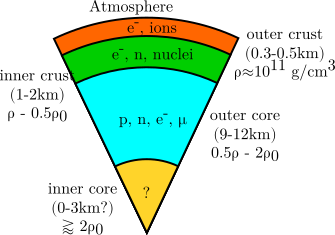
\includegraphics[width=0.5\textwidth]{04_Introduction/Images/pulsar_wind_nebula/pulsar_structure.png}
	\caption{The neutron star/pulsar structure is composed of an inner \& outer core, inner \& outer crust and an atmosphere \citep{2007ASSL..326.....H}.}
	\label{fig:chapter1_pulsar_structure}
\end{wrapfigure}

In 1967 Jocelyn Bell and Antony Hewish observed a series of radio pulses every $1.33\si{\second}$ originating from the same location in the night sky. The object was label LGM-1, short for `little green men' and eventually, became the first known neutron star/pulsar. First proposed by Walter Baade and Fritz Zwicky in the 1930's \citep{1934PhRv...46...76B}, neutron stars are the rotating, highly dense, magnetised remnants of massive stars that emits a beam of photons from its magnetic poles. The magnetic and rotational axes do not necessarily align and the beams of photons rotate around the neutron star. A neutron star is a pulsar when the beam of light points in the direction of earth, forming the characteristic pulse.
\par~\par
Neutron stars are formed during a supernova when a massive star ($\gtrsim 8~M_\odot$) can no longer able support the immense gravitational pressure due to accumulation of iron in the core and undergoes core collapse. Gravitational pressure overcomes electron-degeneracy pressure, forcing electrons and protons in the core to combine to form neutrons. At this point, neutron-degeneracy and the strong force prevents further collapse and the neutron star is created. If the neutron star mass exceeds the Tolman–Oppenheimer–Volkoff limit ($1.5-3~M_\odot$), further collapse can result in a black hole \citep{1996A&A...305..871B, 2015SSRv..188..187S}.
\par~\par
Neutron stars have a mass of $1-3~M_\odot$, average density $\rho_0=2.8\times 10^{14}\si{\gram\per\centi\meter\cubed}$ (nuclear saturated mass density) and a radius $10-15~\si{\kilo\meter}$ which is subdivided into the following layers (see \autoref{fig:chapter1_pulsar_structure}) \citep{2007ASSL..326.....H}: the \textbf{atmosphere} consists of a thin layer of plasma (electrons and light nuclei) up to $10~\cm$ thick with temperature around $10^5-10^6~\si{\kelvin}$ \citep{2002nsps.conf..263Z}. The magnetic field of $10^{11}-10^{14}~\si{G}$ controls the dynamics of the atmosphere. Ions and electrons make up the \textbf{outer crust} in a layer of $0.3-0.5~\km$ thickness of density $\rho=4\times 10^{11}~\si{\gram\per\centi\meter\cubed}$. Just below the atmosphere, a thin non-degenerate electron gas form the edges of the outer crust. This gives way to a liquid/solid crust where nuclei undergo electron capture forming neutrons. The \textbf{inner crust} is around $1~\km$ thick and has average density of $0.3-0.5\rho_0$. The inner crust is composed of electrons, neutrons and neutron-rich nuclei. Both the inner and outer crust have been postulated to contain `nuclear pasta', degenerate matter where neutrons and electrons arrange themselves into complex structures \citep{PhysRevC.88.065807}. The \textbf{outer core} is the thickest part of the neutron star at around $9-12~\km$ thick and has density $0.5-2.0\rho_0$. The \textbf{inner core} exists at the centre of the more massive neutron stars with conditions so extreme, it has been postulated that protons and neutrons break up into their constituent quarks \citep{2007ASSL..326.....H}.
\begin{figure}[ht]
	\centering
	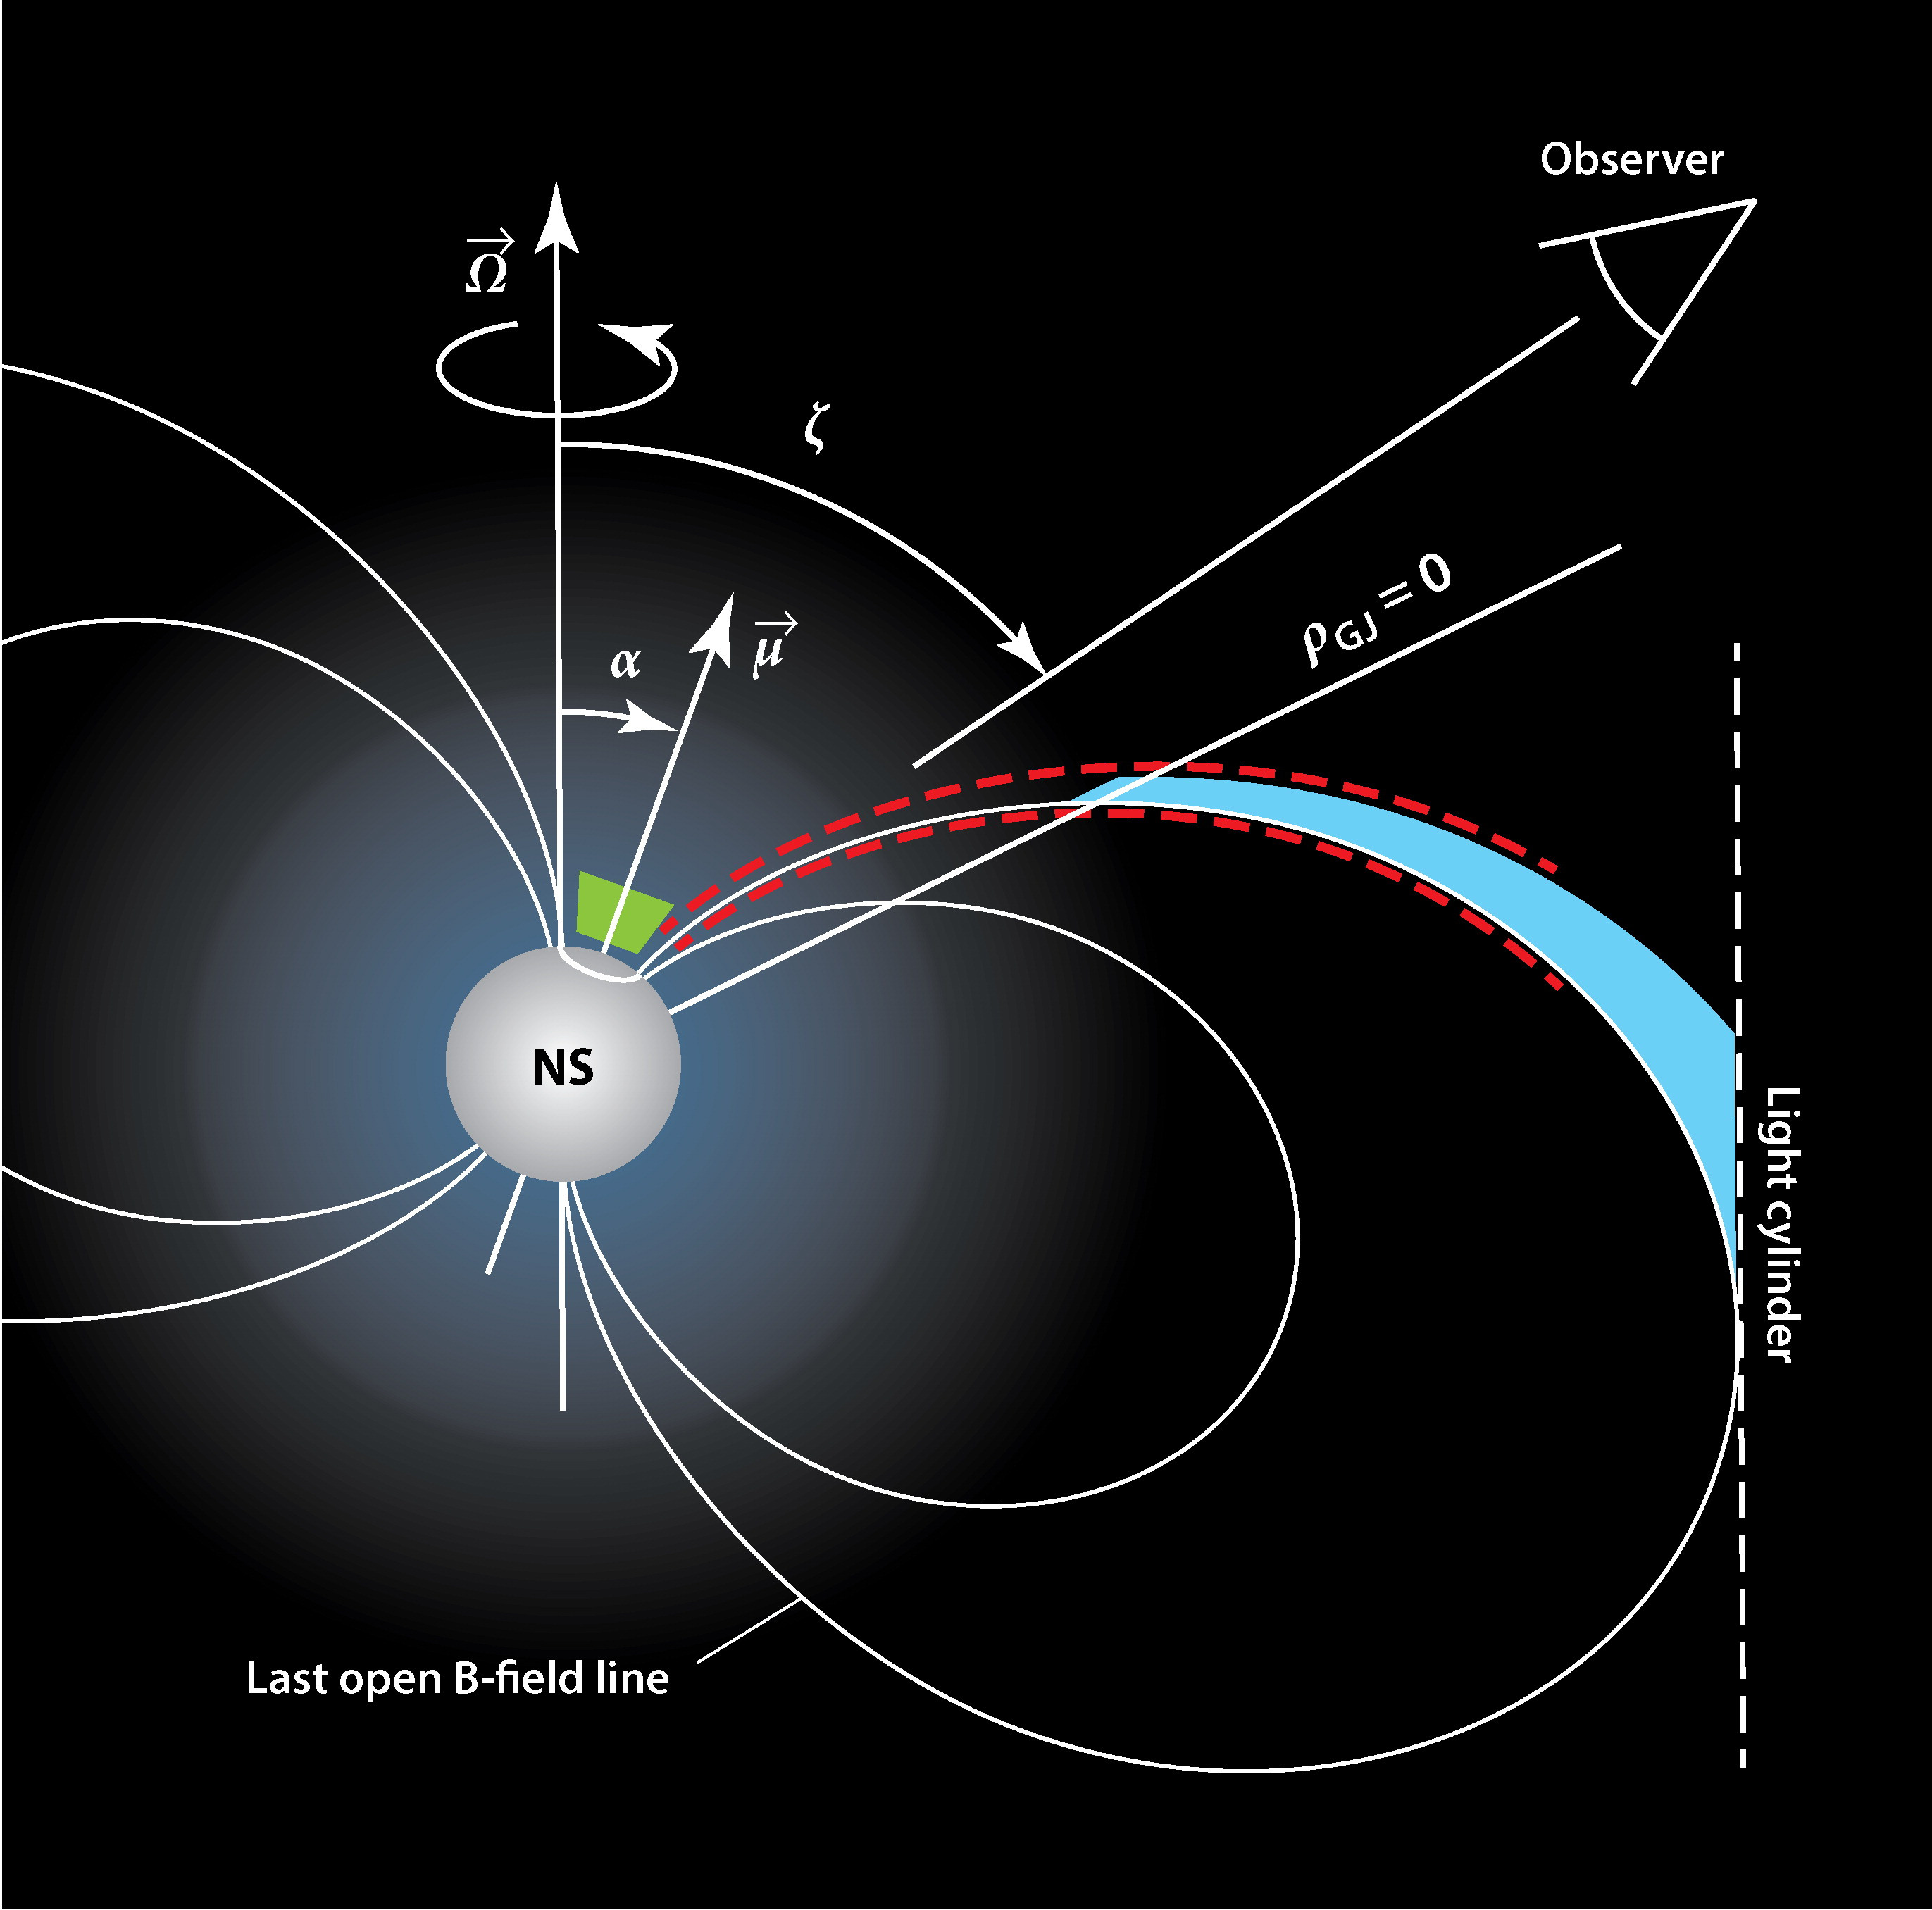
\includegraphics[width=0.7\textwidth]{04_Introduction/Images/pulsar_wind_nebula/pulsar.jpeg}
	\caption{Magnetosphere structure of a pulsar with spin velocity $\vec{\Omega}$ at angle $\alpha$ to the magnetic field axis and angle $\zeta$ to the observer. The acceleration site for the polar cap model and outer gap model is shown in green and blue respectively while the site for the slot gap model is enclosed by the red-dashed lines. Image courtesy of \cite{2014ARA&A..52..211C}.}
	\label{fig:chapter1_magnetosphere_structure}
\end{figure}
\par~\par
After core collapse, pulsars retain the majority of a progenitor star's angular momentum ($L=m\omega r$; \mbox{$m$ = mass}, \mbox{$\omega$ = spin velocity} and \mbox{$r$ = radius}), leading to the pulsar spinning rapidly on its axis. Based on the assumption that the magnetic flux of the progenitor star is conserved, \cite{1964ApJ...140.1309W} proposed that the pulsar's magnetic field could be as strong as $10^{14}-10^{16}~\si{G}$. The rotation coupled with the magnetic field, $\vec{B}$, generates an electric field given by:

\begin{equation}
    \begin{aligned}
    \vec{E} &= \vec{v} \times \vec{B}\text{ ,}
    \end{aligned}
\end{equation}
where $\vec{v}$ is the linear velocity of rotation. The magnetic field rips particles from the surface of the pulsar to form the magnetosphere \cite{1968Natur.218..731G,1969ApJ...157..869G}. The magnetosphere of the pulsar extends out to the light cylinder of radius $R_\text{LC}$:
\begin{equation}
    \begin{aligned}
    R_\text{LC}=c/\Omega\text{ ,}
    \end{aligned}
\end{equation}
where $c$ is the speed of light and $\Omega$ is the angular frequency of the pulsar.
\par~\par
To explain the pulsed radio and gamma-ray emission from the pulsar, \cite{1971ApJ...164..529S} developed the polar-cap model where particles are accelerated at the poles of the pulsar (see \autoref{fig:chapter1_magnetosphere_structure}) and interact with the magnetic field to produce an electron-positron pair ($e^-e^+$). The electron-positron pair emit photons via synchrotron radiation, which then produce a second electron-positron pair. This process cascades until the produced photon can no longer undergo pair production and contributes to the beamed radio emission. The polar-cap model predicts gamma-ray emission due to synchrotron and inverse Compton scattering from the $e^-e^+$ pair. The slot-gap model \citep{1983ApJ...266..215A} extends the acceleration site to higher altitudes until the last open magnetic field line (see \autoref{fig:chapter1_magnetosphere_structure}). The outer-gap model predicts gamma-ray emission due to particle acceleration between the region where $\vec{\Omega}\cdot\vec{B}=0$ and the light cylinder \citep{1986ApJ...300..500C}.
\par~\par
Over time, the rotational kinetic energy is dissipated at a rate described by:

\begin{equation}
    \begin{aligned}
        \dot{E}&=I\Omega\dot{\Omega}\text{ ,}
    \end{aligned}
\end{equation}
\noindent where $I$ is the moment of inertia of the pulsar and $\dot{\Omega}$ is the time derivative of the angular frequency. Some of the spin down power is channelled into the acceleration of particles by the magnetic field. If the pulsar is treated as a simple magnetic dipole, the energy loss becomes \citep{Slane2017}: 

\begin{equation}
    \begin{aligned}
    \dot{E}&=-\frac{BR^6\Omega^4}{6c^2}\sin^2\alpha\text{ ,}
    \end{aligned}
\end{equation}
where $B$ is the magnetic dipole strength at the poles, $R$ is the radius of the pulsar and $\alpha$ is the angle between the rotational and magnetic axes. The angular frequency decreases over time in a manner described by the braking index of the pulsar, $n$:

\begin{equation}
    \begin{aligned}
    \dot{\Omega} &\propto \Omega^n\text{ .}
    \end{aligned}
\end{equation}

The braking index typically takes values between $2\text{ to }3$, where $n=3$ represents a situation where the pulsar loses all its rotational energy through magnetic dipole radiation \citep{2007Ap&SS.308..317L}. However `glitches' (sudden speed up events that are thought to be due to transfer of angular momentum within the pulsar) may result in a braking index $>3$ \citep{2019MNRAS.489.3810P,2020MNRAS.494.2012P}. In the case where a pulsar does not have a companion star, the characteristic age/spin-down timescale is defined to be (\cite{2007ASSL..326.....H} and references within):

\begin{equation}
    \begin{aligned}
    \tau&=\frac{P}{(n-1)\dot{P}} \text{ ,}
    \end{aligned} \label{eq:chapter1_characteristic_age}
\end{equation}
\noindent where $P$ and $\dot{P}$ are the period and period derivative of the pulsar. If the pulsar has a companion star, the extreme gravitational force of the pulsar can strip the companion of its mass and its angular rotation increases. Therefore, the characteristic age may not reflect the true age of the pulsar. The accretion of matter onto the pulsar is believed to be the origin for millisecond pulsars; pulsars with a period less than $10\si{\milli\second}$ \citep{1982Natur.300..728A}.
\par~\par
At the surface of the pulsar, the magnetic field depends on the period and spin down period (\cite{2012hpa..book.....L} and references within):

\begin{equation}
    \begin{aligned}
    B_s&=3.2\times 10^{19}\qty(P\dot{P})^\half\quad\qty[\si{G}]\text{ .}
    \end{aligned}
\end{equation}
\noindent Pulsars with extremely strong magnetic fields are known as magnetars and may be linked to the origin of short gamma-ray bursts and soft gamma ray repeaters \citep{1992ApJ...392L...9D}. For `regular' pulsars, the surface magnetic field has strength $B=10^{11-13}~\si{G}$ while magnetars have magnetic fields up to $10^{14-15}~\si{G}$ \citep{2007ASSL..326.....H}. Possible theories for the extreme magnetic field of a magnetar include; conservation of magnetic field flux of a star with an extreme magnetic field, collapse of a highly magnetized white dwarf or the magnetic field amplification during the birth of the neutron through a dynamo mechanism (the mechanism where a magnetic field is produced by charged plasma in a rotating celestial body) \citep{1992ApJ...392L...9D, 1993_magnetar, 1996AIPC..366..111D}.
\par~\par
The distance to a pulsar can be determined by considering the line of sight ISM. For ISM with electron density $n_e$, electrons naturally oscillate at plasma frequency, $\omega_p$:

\begin{equation}
    \begin{aligned}
        \omega_p^2&=\frac{4\pi n_ee^2}{m_e}\text{ ,}
    \end{aligned}
\end{equation}
\noindent where $e$ and $m_e$ are the charge and the mass of an electron respectively. A photon (with angular frequency $\omega=2\pi f$) in the interstellar medium (ISM) gas will then propagate with velocity \citep{2011piim.book.....D}:

\begin{equation}
    \begin{aligned}
        v&=c\qty(1-\frac{\omega_p^2}{\omega^2})^{1/2}\text{ .}
    \end{aligned}
\end{equation}
\noindent Therefore, photons of frequencies $\nu_1$ and $\nu_2$ emitted simultaneously by the pulsar will experience a time delay $\Delta t=t_2-t_1$ in a manner related to the ISM. The dispersion measure (DM) is defined to be the integrated column density of free electrons over the distance ($d$) to the pulsar\citep{2011piim.book.....D}:

\begin{equation}
    \begin{aligned}
        DM&= \frac{\Delta t}{4.15~\si{\milli\second}\qty[\qty(\nu_2/\si{\giga\hertz})^{-2}-\qty(\nu_1/\si{\giga\hertz})^{-2}]}\\
        &= \int_0^dn_e \dd{\ell}\text{ .}
    \end{aligned} \label{eq:chapter_1_dispersion_measurement}
\end{equation}
\noindent Combining Galactic models of the free electron density (e.g. \cite{2017ApJ...835...29Y}) with time delay measurements, the distance to the pulsar can then be estimated.
 
\subsection{Time Evolution of Pulsar Wind Nebulae} \label{sec:01_intro_time_ev_PWN}
Charged particles (electrons, positrons, protons and nuclei) from the pulsar escape the magnetosphere (which extends up to the light cylinder, see \autoref{fig:chapter1_magnetosphere_structure}) and form the powerful winds known as a PWN. These charged particles
emit photons isotropically and are not tied to the pulsar beam. Therefore, the PWN emission is said to be `unpulsed'. PWNe typically evolve inside a supernova remnant (SNR) (see \autoref{appendix:snrs}).
\par~\par
The characteristics (e.g. morphology, spectral energy distribution) of a PWN depends on the age of the powering pulsar. The PWN can be divided into three stages: the expansion phase, a compression-expansion phase and the formation of a halo.

\begin{figure*}[h!]
	\centering
	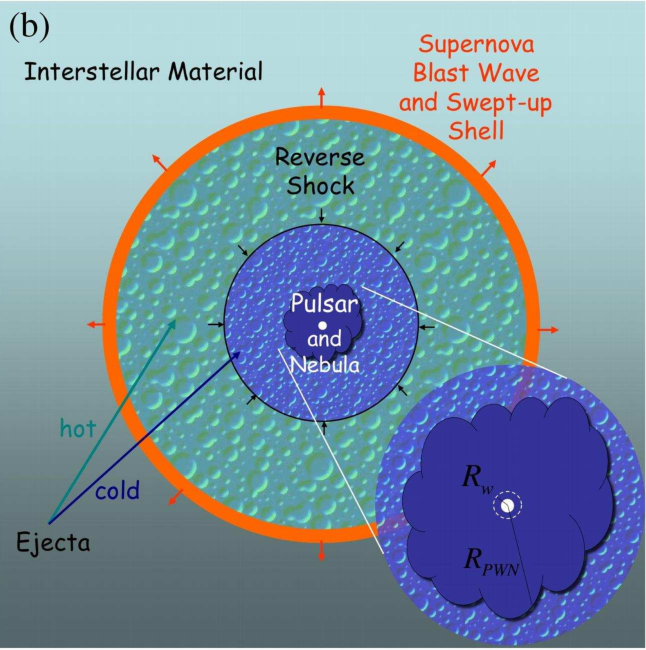
\includegraphics[height=0.4\textwidth]{04_Introduction/Images/pulsar_wind_nebula/pulsar_wind_nebula_structure.pdf}
	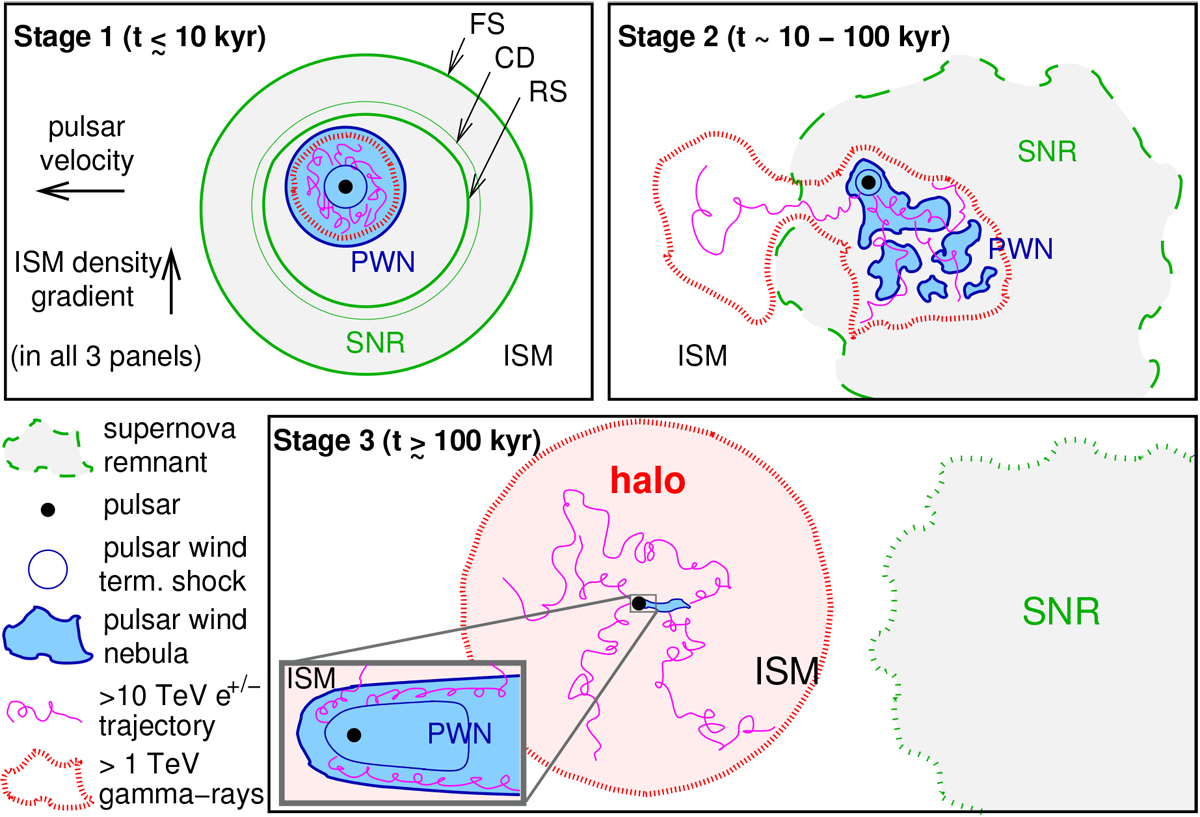
\includegraphics[height=0.4\textwidth]{04_Introduction/Images/pulsar_wind_nebula/pwn_evolution.jpg}
	\caption{(\textit{left}) Structure of a composite SNR and PWN. Image courtesy of \cite{2006ARA&A..44...17G}. (\textit{right}) A PWN evolves within the SNR and is eventually crushed by the reverse shock. The pulsar escapes the SNR and the electrons escaping into the ISM form a TeV halo around the PWN. Image courtesy of \cite{2020A&A...636A.113G}.}
	\label{fig:chapter1_pulsar_wind_nebula_structure}
\end{figure*}

\subsubsection{Stage 1: Expansion Phase ($<10~\si{\kilo\year}$)}

As the pulsar wind expands into the shocked region of the SNR, the outer winds of the PWN are decelerated by the ISM until the ram pressure of the interstellar wind counteracts the internal pressure of the PWN, $P_\text{PWN}$ (see \autoref{fig:chapter1_pulsar_wind_nebula_structure}). This forms the termination shock at radius \citep{2006ARA&A..44...17G}:

\begin{equation}
    \begin{aligned}
    r_\text{ts}&=\qty(\frac{\dot{E}}{4\pi\omega c P_\text{PWN}})^\half\text{ ,}
    \end{aligned}
\end{equation}
where $\dot{E}$ is the spin-down power and $\omega$ is the filling factor of the PWN ($\omega \approx 1$ for isotropic winds) \citep{2002AstL...28..373B}. Typical PWN have a termination shock occurring at $r_s\approx 0.1~\pc$ \citep{2006ARA&A..44...17G}. Particles are re-accelerated at the termination shock and are believed to be the source of the radio to unpulsed $\TeV$ emission from PWN. For a PWN in its first stage of evolution, the radius evolves as \citep{10.1007/978-94-010-1229-4_5}:

\begin{equation}
    \begin{aligned}
    r_\text{PWN} &= 1.5\dot{E_0}^\frac{1}{5}E_\text{SNR}^{\frac{3}{10}}M_\text{ej}^{-\frac{1}{2}} t^\frac{6}{5} \text{ ,}
    \end{aligned}
\end{equation}
where $E_\text{SNR}$ and $M_\text{ej}$ are the energy and ejected mass of the SNR respectively. At this stage the spin down energy of the pulsar, $E_0$, is roughly constant.
\par~\par 
Asymmetry in the progenitor supernova will result in the pulsar gaining a so-called kick velocity of $300~\kmpersec$ \citep{2017ApJ...844....1K}, however at early stages the pulsar appears towards the centre of the SNR. 

\subsubsection{Stage 2: ($10-100~\kiloyear$)}

As the PWN evolves inside the SNR, the outer edges of the SNR collide with the ISM and forms a reverse shock (see \autoref{appendix:snrs}). The reverse shock travels radially inwards and crushes the PWN, increasing its pressure and magnetic field \citep{2006ARA&A..44...17G}. The pressure inside the PWN increases until it is greater than its surroundings, resulting in a subsonic expansion of the nebula. This compression and expansion phase repeats itself over a time scale of a few thousand years. The crushing of the PWN by the reverse shock is anti-symmetric due to the kick velocity of the pulsar and non-uniformity in the ISM, which leads to complex morphology of the PWN.
\par~\par 
At the edge of the PWN, $r_\text{PWN}$, the pressure is balanced with that of the associated SNR. During stage 2, the SNR will be in its Sedov-Taylor phase of its evolution (see \autoref{appendix:snrs}) with radius $r_\text{SNR} \propto t^{\frac{2}{5}}$. Therefore the radius of the PWN is thought to be related to the SNR radius via \citep{2001A&A...380..309V}:

\begin{equation}
    \begin{aligned}
        r_\text{PWN}\propto t^{\frac{1}{3}} r_\text{SNR} = t^{11/15}\text{ .}
    \end{aligned}
\end{equation}
\par~\par
High-energy electrons can escape the PWN into the ISM and can emit $\TeV$ $\gamma$-rays via inverse Compton interactions, forming a $\TeV$ halo \citep{2020A&A...636A.113G}.

\subsubsection{Stage 3: Formation of $\TeV$ halos ($t\gtrsim100~\kiloyear$)}

At this stage, the kick velocity of the pulsar has allowed it to escape the SNR (which is now fading into the ISM). The pulsar is travelling faster than the speed of the sound in the ISM, forming a bow shock with the PWN trailing behind (see \autoref{fig:chapter1_pulsar_wind_nebula_structure}) \citep{2020A&A...636A.113G}. At this point a $\TeV$ halo is formed around the PWN. Extended $\TeV$ emission, indicative of a $\TeV$ halo, has been seen towards the Geminga and \mbox{PSR\,B0656+14} pulsars \citep{2017Sci...358..911A}.

\subsubsection{Time Evolution of the PWN Magnetic Field Structure}

\begin{figure}[h!]
	\centering
    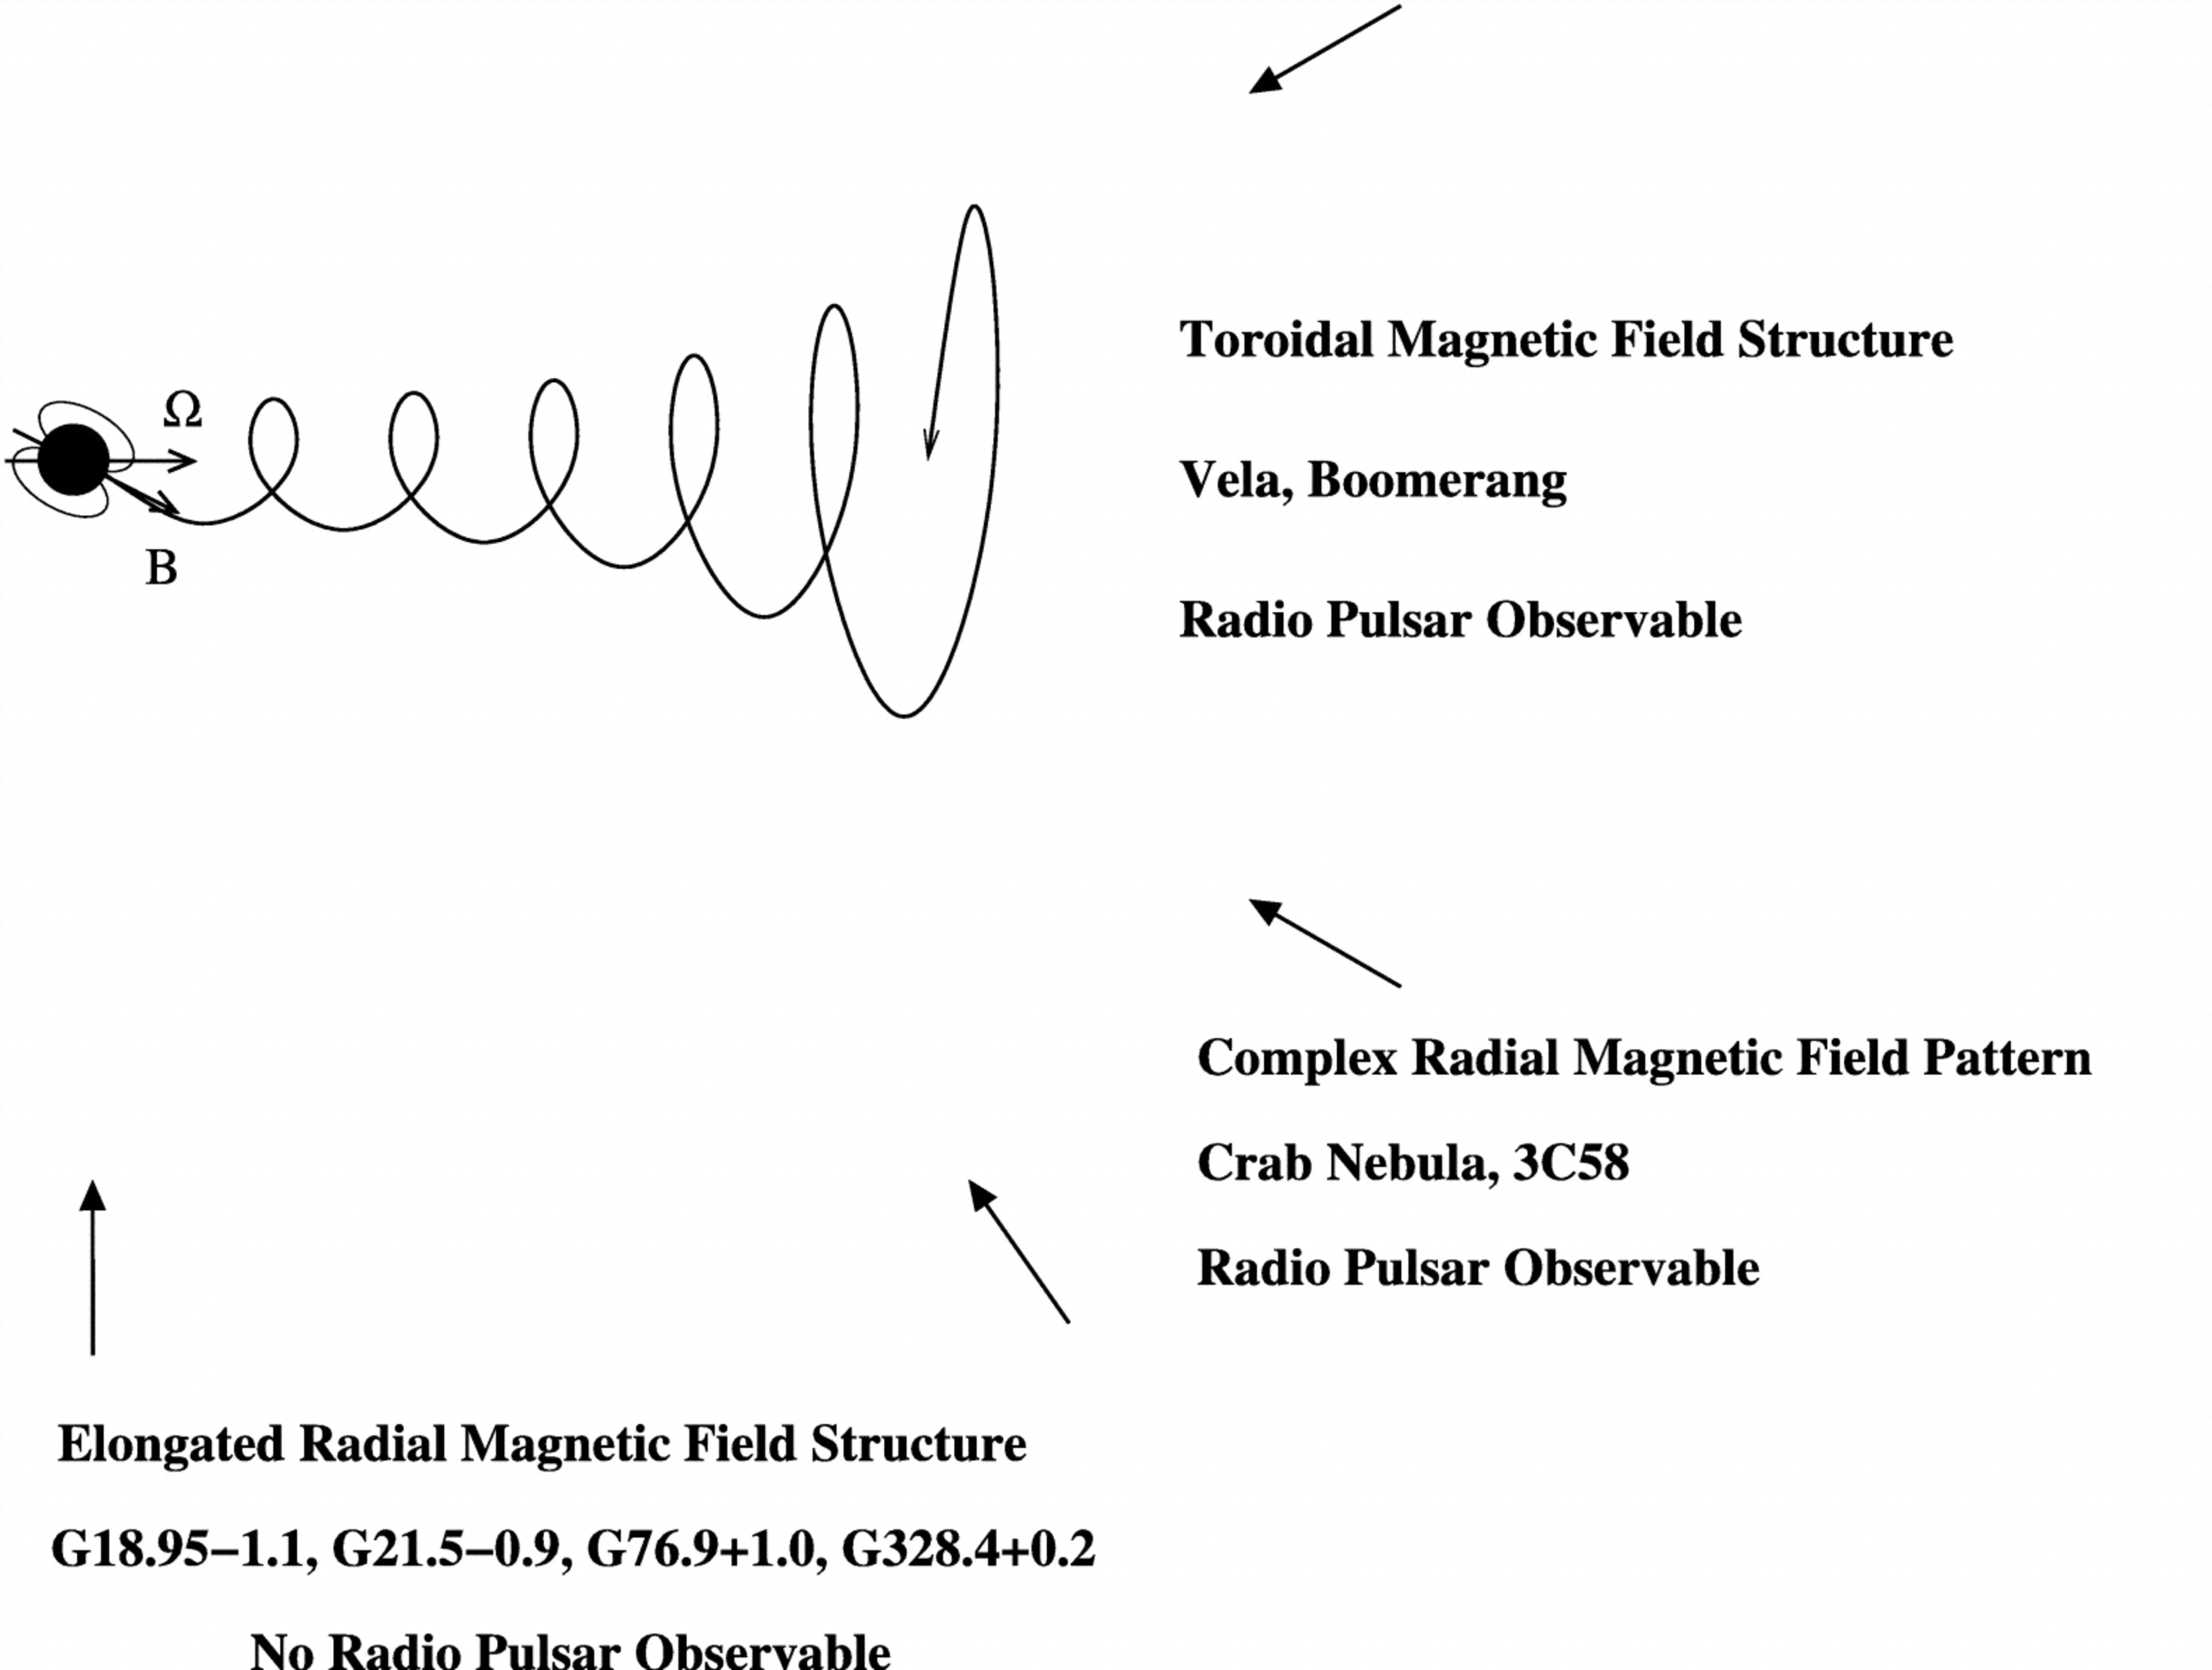
\includegraphics[height=0.22\textheight]{04_Introduction/Images/pulsar_wind_nebula/magnetic_field_structure.pdf}
	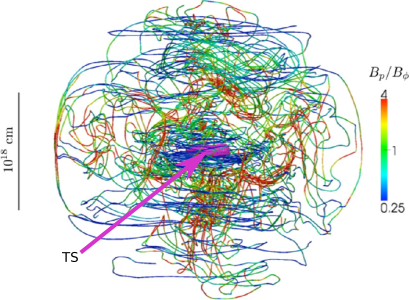
\includegraphics[height=0.22\textheight]{04_Introduction/Images/pulsar_wind_nebula/PWN_magnetic_field_structure.jpeg}
	\caption{(\textit{left}) Expansion of the PWN magnetic field lines and how the viewing angle alters the way the magnetic field structure appears at Earth. Image courtesy of \cite{2006ApJ...638..225K}(\textit{right}) Simulated magnetic field lines of a stage 1 PWN. Azimuthal orientated field lines are shown in blue while radial field lines are shown in red. The termination shock is indicated by magenta and indicated by the arrow. Image adapted from \cite{2014MNRAS.438..278P}}
	\label{fig:chapter1_magnetic_field_structure_PWN}
\end{figure}

The charged winds of PWNe are influenced by the presence of magnetic fields. The magnetic field structure of PWNe is believed to be toroidal in nature, with the viewing angle affecting observations at Earth \citep{2006ApJ...638..225K, 2012SSRv..166..231R}. If the axis of rotation aligns with the viewing angle, the magnetic field appears to be toroidal (see left hand panel of \autoref{fig:chapter1_magnetic_field_structure_PWN}). In contrast, the magnetic field of the pulsar will appear to be radially dependent if the viewing angle and axis of rotation is perpendicular to each other. More complex observed magnetic field structures occur when the viewing angle is between these two extremes (see the right hand panel of \autoref{fig:chapter1_magnetic_field_structure_PWN}).
\par~\par
The magnetic field evolves with the PWN. The average magnetic field of the PWN, $B_\text{PWN}$, at time $t$ can be found by considering the conservation of magnetic energy density (see \cite{2010ApJ...715.1248T} and references within):

\begin{equation}
    \begin{aligned}
    V_\text{PWN}\frac{B^2_\text{PWN}\qty(t)}{8\pi}&=\int_0^t\eta L\qty(t')\dd{t'} \\
    &=\eta E_\text{spin}\qty(t)\text{ ,}
    \end{aligned} \label{eq:chapter_1_magnetic_conservation_energy}
\end{equation}
\noindent where $V_\text{PWN}$ is the volume of the PWN, $L$ is the injection luminosity (of particles) of the PWN, $\eta$ ($0\leq\eta\leq 1$) is the ratio of the magnetic energy and the pulsars' spin down power and $E_\text{spin}$ is the time-integrated spin down energy. The resulting magnetic field is then:

\begin{equation}
    \begin{aligned}
    B\qty(t)&=\sqrt{\frac{3\qty(n-1)\eta L_0\tau_0}{R^3_\text{PWN}}\qty[1-\qty(1+\frac{t}{t_0})^{-\frac{2}{n-1}}]}\text{ ,}
    \end{aligned} \label{eq:chapter_1_magnetic_field_ev}
\end{equation}
\noindent where $R_\text{PWN}$ is the size of the PWN and $\tau_0$ is the initial spin down timescale (see \autoref{eq:chapter1_characteristic_age}). For $t>\tau_0$, the magnetic field of the PWN can be approximated by $B\qty(t)\propto t^{-1.5}$.

\subsubsection{Time Evolution of the Spectral Energy Distribution}

\begin{figure}[h!]
    \centering
    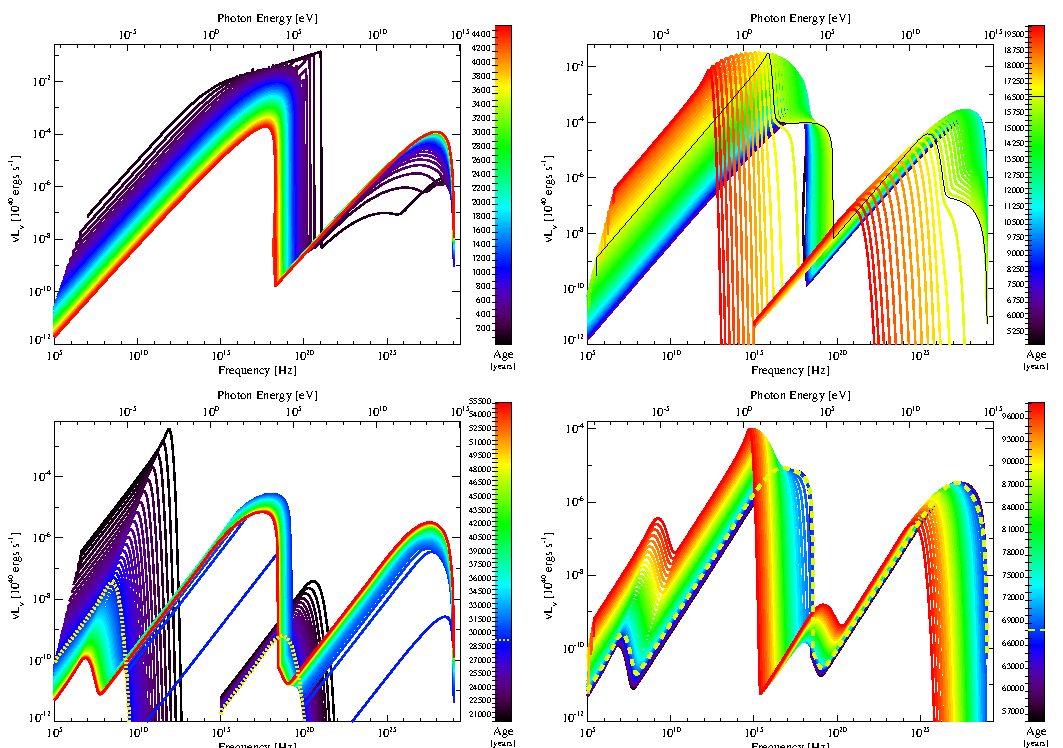
\includegraphics[width=\textwidth]{04_Introduction/Images/pulsar_wind_nebula/pwn_spectra_evolution.pdf}
    \caption{Theoretical time evolution of the multi-wavelength SED of a PWN inside a SNR. See text for more information. Image courtesy of \cite{2009ApJ...703.2051G}.}
    \label{fig:chapter_1_PWN_spectra_evolution}
\end{figure}
A spectral energy distribution (SED) describes how the energy flux of photons (or particles) from a source varies with energy. \autoref{fig:chapter_1_PWN_spectra_evolution} from the study \cite{2009ApJ...703.2051G} shows the SED time evolution for an example PWN with braking index $3$ and electron injection luminosity of $10^{40}~\ergspersec$, where electrons follow a power-law spectrum ($\propto E^{-1.6}$).
\par~\par
At $t=0$ (stage 1), the injected electrons have not experienced any energy losses and form a strong peak in the X-ray regime through synchotron emission. The same electrons will interact with the cosmic microwave background (CMB) through inverse Compton interactions and form a strong peak in the $\GeV$ regime  (top-left panel of \autoref{fig:chapter_1_PWN_spectra_evolution}). As the PWN expands within the SNR, the overall magnetic field strength of the PWN decreases and the synchotron luminosity peak migrates to lower energies in the optical regime. This leaves more energy to be lost through inverse Compton (IC) interactions (see \autoref{sec:chapter_1_leptonic_gre}) and the IC peak transitions from the $\GeV$ to the $\TeV$ regime.
\par~\par
As the reverse shock compresses the PWN (stage 2), the increased magnetic field turbulence within the PWN strengthens the magnetic field. Thus, electrons injected into the PWN lose more energy to synchrotron losses and the ratio of synchrotron to IC flux increases (top-right panel of \autoref{fig:chapter_1_PWN_spectra_evolution}). At this point, two distinct peaks start to form in the synchrotron and inverse Compton spectra due to the two populations of young high-energy electrons and the older lower energy electrons that were initially injected into the PWN. During this compression, the pulsar may leave the PWN and no new electrons are injected into the system. The synchrotron and IC peak from the young high electrons subsequently disappears (black line in the top-right panel of \autoref{fig:chapter_1_PWN_spectra_evolution}).
\par~\par
The pressure inside the PWN increases due to compression until is greater than the surrounding ISM and the PWN expands. Before the pulsar re-enters the PWN, the overall magnetic field strength of the PWN decreases and the IC flux from the`  electron population increases at the expense of the synchrotron flux (top-right and bottom-left panel of \autoref{fig:chapter_1_PWN_spectra_evolution}). New electrons are injected in the PWN when the pulsar re-enters the system, creating two populations of old low-energy electrons and young high-energy electrons. This is reflected in the IC and synchrotron emission (dotted orange line in the bottom-left panel of \autoref{fig:chapter_1_PWN_spectra_evolution}).
\par~\par
As the PWN re-expands, the pressure inside the PWN decreases until it less than the pressure due to the associated SNR and the PWN is compressed. Similarly to the the first compression, the magnetic field strength inside the PWN increases and the ratio of synchrotron to IC flux increases. The pulsar will again leave the PWN (dotted yellow line in the bottom right-panel of \autoref{fig:chapter_1_PWN_spectra_evolution}) and no new electrons are injected into the system (stage 3). The synchrotron and IC peak from the young high-energy electrons migrates to lower energies due to high energy losses. However, the energy of the synchotron peak from old low-energy electrons increases while the energy of the IC peak decreases as a result of the increasing magnetic field.

\subsection{TeV Pulsar Wind Nebula} \label{sec:01_PWN_TeVPWN}

It was postulated by \cite{1965PhRvL..15..577G} that PWN are a source of $\TeV$ gamma rays via IC emission, but it wasn't until \cite{1989ApJ...342..379W} reported the first detection of $\TeV$ emission from the Crab Nebula. A $\TeV$ PWN is predicted to be physically larger than the X-ray nebula \citep{1997MNRAS.291..162A}.

\begin{figure}[h!]
	\centering
	\begin{subfigure}{0.495\textwidth}
	    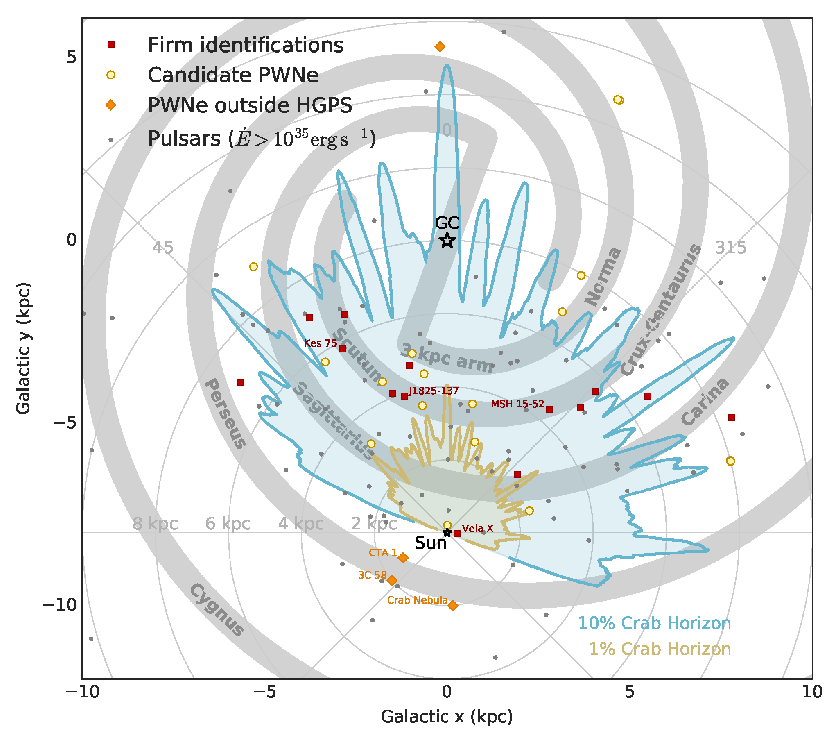
\includegraphics[width=\linewidth]{04_Introduction/Images/pulsar_wind_nebula/TeV_PWN_location.eps}
	\end{subfigure}
	\hfill
	\begin{subfigure}{0.495\textwidth}
	    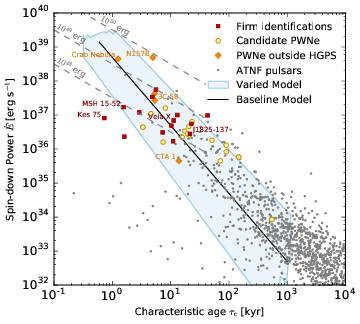
\includegraphics[width=\linewidth]{04_Introduction/Images/pulsar_wind_nebula/pulsar_spin_down_vs_age.png}
	\end{subfigure}
	
	\begin{subfigure}{0.495\textwidth}
	    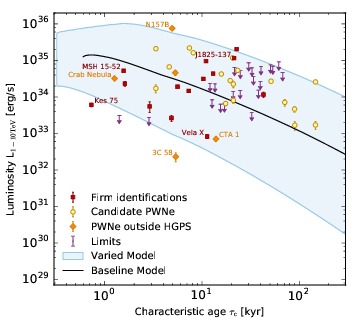
\includegraphics[width=\linewidth]{04_Introduction/Images/pulsar_wind_nebula/pulsar_luminosity_vs_age.png}
	\end{subfigure}
	\hfill
	\begin{subfigure}{0.495\textwidth}
	    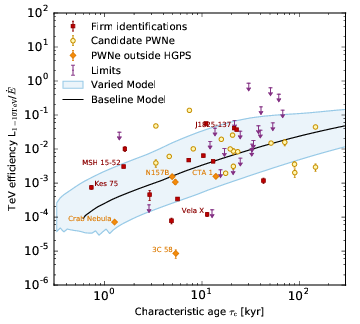
\includegraphics[width=\linewidth]{04_Introduction/Images/pulsar_wind_nebula/pulsar_efficiency_vs_age.png}
	\end{subfigure}
	\caption{(\textit{top-left}) An illustration of the Milky Way spiral arm structure and the location of identified and candidate PWN from the H.E.S.S. HPGS. Spin down power (\textit{top-right}), $\TeV$ luminosity (\textit{bottom-left}) and $\TeV$ efficiency (\textit{bottom-right}) vs the characteristic age of known PWN. Images from  \cite{2018A&A...612A...2H}.}
	\label{fig:chapter1_PWN_properties}
\end{figure}
\par~\par
The H.E.S.S. $\TeV$ gamma-ray survey revealed 78 very high-energy (VHE) gamma-ray sources \citep{2018A&A...612A...1H}: 12 are confirmed $\TeV$ PWNe, 8 are composite objects (PWN + SNR) and a further 36 are identified as $\TeV$ PWNe candidates. The H.E.S.S. observatory will be discussed further in \autoref{sec:02_HESS}. \cite{2018A&A...612A...2H} reviewed the H.E.S.S. Galactic Plane Survey (HPGS) in order to investigate the evolution and nature of TeV PWNe. It was found that the majority of PWN are located on or near the Milky Way spiral arms, with the Crux-Scutum arm hosting half of the PWN from the HGPS (see \autoref{fig:chapter1_PWN_properties}).
\par~\par
Through time-dependent modelling of $\TeV$ PWN, \cite{2018A&A...612A...2H}, it was noted that as PWNe age:

\begin{enumerate}
    \itemsep0em
    \item The physical offset between the pulsar and TeV PWN increases (at a rate of $\approx 0.5\si{pc\per\kilo\year}$) due to the kick-velocity of the pulsar and the SNR reverse shock crushing the PWN.
    \item The TeV luminosity ($L_{1-10~\TeV}$) of known PWN varies widely with characteristic age (from $\approx 10^{35}~\ergspersec$ at $1~\kiloyear$ to $\approx 10^{34}~\ergspersec$ at $10~\kiloyear$) with no clear statistical correlation.
    \item The TeV efficiency ($L_{1-10~\TeV}/\dot{E}$) increases (from $2\times 10^{-4}$ at $1~\kiloyear$ to $3\times 10^{-3}$ at $10~\kiloyear$) possible due to the physical offset between the pulsar and TeV PWN.
\end{enumerate}

\subsection{Mysteries of Pulsar Wind Nebulae} \label{sec:chapter_1_mystery_PWN}

Even though multiple PWNe have been observed and studies such as \cite{2018A&A...612A...2H} have modelled trends of $\TeV$ PWN, there are still many open questions. The following will summarise some of these questions.

\subsubsection{How are electrons transported within pulsar wind nebula?}

Electrons released by a pulsar are subject to varying transportation processes and energy losses. In a non-uniform environment (due to gas and magnetic field turbulence), electrons scatter off the ISM atoms and magnetic field turbulence resulting in diffusive motion outwards from the acceleration site (see \autoref{chapter_1_cr_propagation}). Electrons in PWNe may also experience an overlying bulk transport in a particular direction, i.e. advection. It has been proposed that advection dominates the particle transport close to the pulsar while diffusion dominates the outer reaches of the nebula \citep{2020A&A...636A.113G, 2021PhRvD.104l3017R}. Electrons undergo energy loss through inverse-Compton, synchrotron and Bremsstrahlung emission (see section \autoref{sec:chapter_1_leptonic_gre}). The rate at which an electron loses energy depends heavily on the surrounding environment.
\par~\par
A challenge in modelling PWN will be balancing the transportation of electrons and energy losses with respect to the surrounding environment to order to explain the multiwavelength emission.

\subsubsection{Can pulsar wind nebula accelerate particles up to $\PeV$ energies?}

The break between the knee ($1~\PeV=10^{15}~\eV$) and the ankle ($10^{18}~\si{\exa\electronvolt}$) in the cosmic ray proton and nuclei spectrum at Earth suggests the transition from Galactic to extra-Galactic cosmic rays (see \autoref{sec:chapter_1_cr_spectrum}). Thus, what type of Galactic source is capable of accelerating cosmic rays up to PeV energies, i.e. a PeVatron?
\par~\par
Due to their large energy budget ($\approx 10^{51}~\ergs$ of kinetic energy) and production rate ($\approx 2-3$ supernova occur in the Milky Way per century), SNRs have been the most likely candidates for Galactic PeVatrons \citep{1983A&A...125..249L, 1984ARA&A..22..425H,2004MNRAS.353..550B,10.1093/mnras/sty1589}. Recently, the suitability of SNRs by themselves as PeVatrons has been called into question \citep{CRISTOFARI2020102492} and PWNe are now being considered as additional candidates \citep{2018MNRAS.478..926O, Xin_2019, de_O_a_Wilhelmi_2022,2022A&A...660A...8B}.
\par~\par
In 2021, the LHAASO facility identified 12 gamma-ray sources with the detection of photons between $100~\TeV$ to $1.4~\PeV$ \citep{2021Natur.594...33C}. These sources are prime PeVatron candidates; two being firmly identified PWNe and a further nine having possible PWN counterparts. One of the twelve PeVatron candidates is the Crab Nebula. The $\MeV$ synchrotron emission from the Crab Nebula and maximum gamma-ray energy of $\approx 0.9~\PeV$ heavily implies the presence of $\PeV$ electrons within the nebula \citep{doi:10.1126/science.abg5137}.

\subsubsection{Is there a hadronic component to the pulsar wind nebula?}

Spectral and spatial analysis of known PWNe indicate that leptonic emission is the main source of gamma-ray emission. With the detection of $\PeV$ emission towards known PWNe \citep{doi:10.1126/science.abg5137}, further studies suggest that PWN may have an additional hadronic component \citep{10.1111/j.1745-3933.2010.00934.x, Xin_2019, 2021ApJ...922..221L}. The majority of literature consider the winds of the PWN to consist of electrons and positrons (e.g. \cite{2018A&A...612A...2H}). However, in the polar cap model (see \autoref{fig:chapter1_magnetosphere_structure}) electrons, positrons and protons are stripped from the surface of the pulsar. \cite{1994ApJ...435..230G} proposed that a fraction of the spin-down power of the pulsar is converted into a wind of protons. These protons undergo proton-proton collisions to produce pions (see \autoref{sec:chapter1_hadronic_gr_emission}). Charged pions decay into muons, which subsequently decay into electrons and positrons. \cite{2003A&A...402..827A} suggested that signatures of these `secondary' electrons/positrons can be found in the production of $\TeV$ gamma rays and neutrinos. Moreover, the SNR reverse shock can re-introduce protons into the PWN and accelerate protons greater than $1~\PeV$ \citep{1992MNRAS.257..493B,2018MNRAS.478..926O}.


\subsection{HESS J1825-137 and HESS J1826-130} \label{sec:01_1825_1826}

% 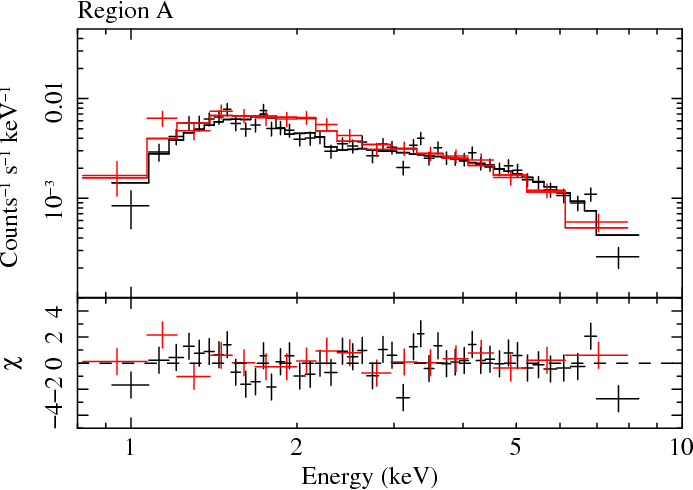
\includegraphics[width=0.5\textwidth]{04_Introduction/Images/pulsar_wind_nebula/1825_xray_flux.png}

This thesis will focus on the PWN associated with $\TeV$ source \mbox{HESS\,J1825-137}. The following will briefly summarise the literature of \mbox{HESS\,J1825-137} and nearby $\TeV$ source \mbox{HESS\,J1826-130}.

\begin{figure}[h!]
	\centering
	% 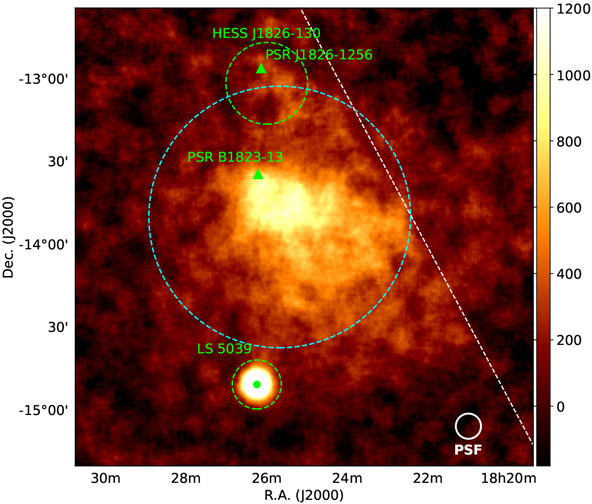
\includegraphics[height=0.23\textheight]{04_Introduction/Images/pulsar_wind_nebula/1825_morphology.jpg}
	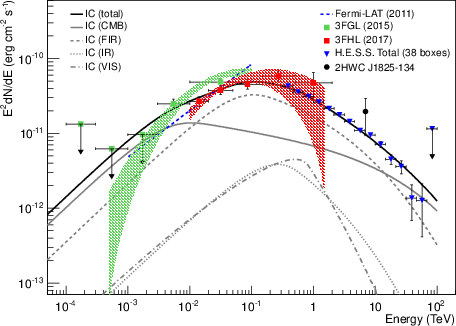
\includegraphics[height=0.2\textheight]{04_Introduction/Images/pulsar_wind_nebula/1825_energy_flux.png}
    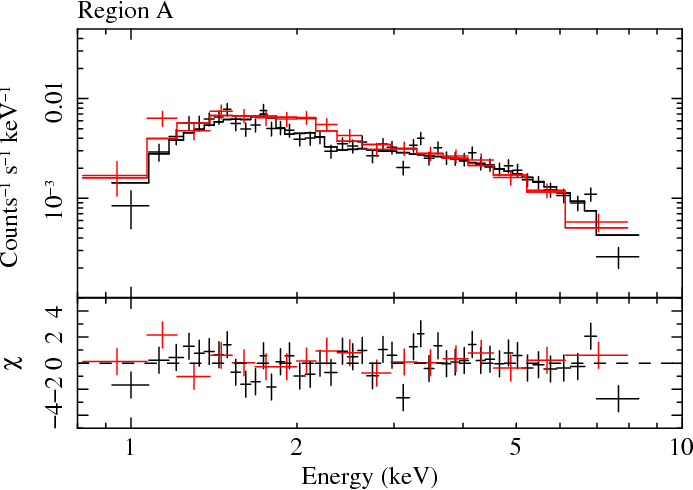
\includegraphics[height=0.2\textheight]{04_Introduction/Images/pulsar_wind_nebula/1825_xray_flux.png}
    \caption{(\textit{left}) Gamma-ray SED of \mbox{HESS\,J1825-137} as seen by HESS together with the \textit{Fermi}-LAT 3FGL and 4FHL equivalent sources. (\textit{right}) X-ray SED towards \mbox{PSR\,J1826-1334}. Images courtesy of \cite{2019A&A...621A.116H} and \cite{2009PASJ...61S.189U}.}
    \label{fig:chapter1_hess_j1825_morphology_paramaters}
\end{figure}

\begin{SCfigure}[0.67][h!]
    \centering
    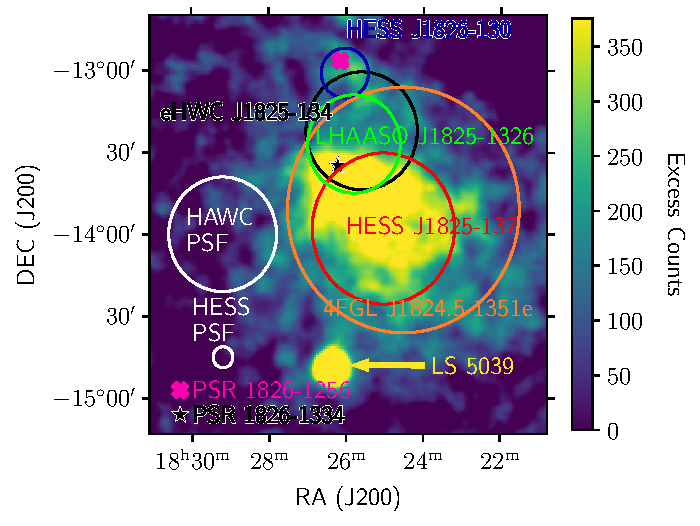
\includegraphics[width=0.6\textwidth]{04_Introduction/Images/pulsar_wind_nebula/hess_j1825_image.pdf}
    \caption{HESS excess counts map towards \mbox{HESS\,J1825-137} from \cite{2019A&A...621A.116H}. The spatial position and extent of \mbox{HESS\,J1825-137} and the equivalent \textit{Fermi}-LAT, HAWC and LHAASO sources are shown together with PSR\,J1826-1334 (star) and PSR\,J1826-1256 (cross).}
    \label{fig:chapter1_hess_j1825_137_object_positions}
\end{SCfigure}


\begin{table}[h!]
    \caption{Fit parameters to the spectrum of \mbox{HESS\,J1825-137} and equivalent \textit{Fermi}-Lat and HAWC sources. Power law (PL): $\dv{N}{E}\propto \qty(\frac{E_p}{E_0})^{-\Gamma}$. Exponential Cutoff Power Law (ECPL): $\dv{N}{E}\propto \qty(\frac{E_p}{E_0})^{-\Gamma}\exp(-\frac{E}{E_c})$. Log Parabola (LP): $\dv{N}{E}\propto \qty(\frac{E_p}{E_0})^{-\Gamma+\beta\log(E/E_0)}$. Broken Power Law (BPL: $\dv{N}{E}\propto \qty(\frac{E_p}{E_b})^{-\Gamma}$ where $\Gamma=\Gamma_1$ if $E<E_b$ and $\Gamma=\Gamma_2$ otherwise. $E_0=1~\TeV$ unless specified.}
    \resizebox{\textwidth}{!}{
    \begin{threeparttable}
    \centering
    \begin{tabular}{rllllll}
        \toprule
        Model & $\Gamma$ & Parameters & RA & DEC & extent ($^\circ$) & References \\
        \midrule 
        \textbf{HESS J1825-137} & - & - & $18\si{\hour}25\si{m}49\si{\second}$ & $-\ang{13}46\si{m}35\si{\second}$ & $0.66^*$ & a \\
        PL & $2.23\pm0.02\pm0.04$ & - & - & - & - & a \\
        ECPL & $2.06\pm0.05\pm0.08$ & $E_c = 15\pm5\pm6~\TeV$ & - & - & - & a \\
        LP &  $2.21\pm0.03\pm0.04$ & $\beta=0.08\pm 0.02\pm 0.03$ & - & - & - & a \\
        \textbf{4FGL\,J1824.5-1351e} & - & - & $18\si{\hour}24\si{m}31.2\si{\second}$  & $-\ang{13}51\si{m}07.2\si{\second}$  & $0.75$ & b \\
        LP & $1.96\pm0.68$ & $E_0 = 145\pm~\GeV$ & - & - & - & c \\
        & - & $\beta$ = $0.046\pm 0.013$ & - & - & - & - \\
        BPL & $1.70\pm0.04$ & $E_b = 115\pm8~\GeV$ & - & - & - & c \\
        & $2.29\pm0.15$ & - & - & - & - & - \\
        \textbf{3HWC J1825 - 134} & - & - &  $18\si{\hour}25\si{m}50.4\si{\second}$ & $-\ang{13}24\si{m}03.6\si{\second}$ & - & d  \\
        PL & $2.35\pm0.02$ & - & - & - & - & d \\
        \textbf{eHWC J1825 - 134} & - & - &  $18\si{\hour}25\si{m}36\si{\second}$ & $-\ang{13}22\si{m}12\si{\second}$ & $0.34$ & e  \\
        ECPL  & $2.12\pm0.15$ & $E_c = 61\pm12~\TeV$  & - & - & - & e \\
        \textbf{LHAASO\,1825-1326} & - & - & $18\si{\hour}25\si{m}48\si{\second}$ & $-\ang{13}27\si{m}00\si{\second}$ & $0.3$ & f \\
        \bottomrule
    \end{tabular}
    \begin{tablenotes}
	\item $^*$: Average of the southern and northern extent 
	\item \textbf{References}
	\item a: \citep{2019A&A...621A.116H}
	\item b: \citep{2020ApJS..247...33A}
	\item c: \citep{2020A&A...640A..76P}
	\item d: \citep{2020ApJ...905...76A}
	\item e: \citep{PhysRevLett.124.021102}
    \item f: \citep{2021Natur.594...33C}
    \end{tablenotes}
    \end{threeparttable}
    }
    \label{tab:chapter1_1825_parameters}
\end{table}

Discovered in $2005$, \mbox{HESS\,J1825-137} is one of the most luminous and extensive $\TeV$ PWN \citep{2005A&A...442L..25A,2006A&A...460..365A}. \mbox{HESS\,J1825-137} is powered by \mbox{PSR\,J1826-1334}, which has a spin down power, period, period derivative and DM distance of $2.8\times 10^{36}~\ergspersec$, $101.5~\si{\milli\second}$, $7.5\times 10^{-14}~\si{\second\per\second}$ and $3.6~\kpc$ respectively \citep{2005AJ....129.1993M}. \autoref{eq:chapter1_characteristic_age} gives the characteristic age of PSR\,J1826-1334 as $21.4~\si{\kiloyear}$, placing the PWN in its second phase of its evolution (see \autoref{sec:01_intro_time_ev_PWN}). In support of this, a $\TeV$ halo appears to be forming around \mbox{HESS\,J1825-137} \citep{2020A&A...640A..76P}. The High Altitude Water Cherenkov (HAWC) observatory has observed gamma-rays towards equivalent source \mbox{eHWC\,J1825-134} with energies greater than $100~\TeV$ \citep{PhysRevLett.124.021102}. Similarly, LHAASO identified \mbox{HESS\,J1825-137} (LHAASO\,J1825-1326) as a possible PeVatron candidate (see section.\,\autoref{sec:chapter_1_PeVatrons}) \citep{2021Natur.594...33C}. The equivalent $\GeV$ \textit{Fermi}-LAT source is \mbox{4FGL\,J1824.5-1351e}.  See \autoref{tab:chapter1_1825_parameters} and \autoref{fig:chapter1_hess_j1825_137_object_positions} for the spectral and spatial information of \mbox{HESS\,J1825-137} and equivalent sources.
\par~\par
The $\TeV$ morphology towards \mbox{HESS\,J1825-137} (see \autoref{fig:chapter1_hess_j1825_137_object_positions}) is asymmetric around the pulsar, with more extensive emission towards the southern side of the nebula (in Galactic coordinates). The extent (defined to be the point at which the emission drops to $1/e$ of its highest value) towards the south of \mbox{HESS\,J1825-137} was found \citep{2019A&A...621A.116H} to be $\ang{0.66}\pm\ang{0.03}_\text{stat}\pm\ang{0.04}_\text{sys}$, while the northern side is extended by $\ang{0.41}\pm\ang{0.03}_\text{stat}\pm\ang{0.09}_\text{sys}$. At a distance of $4.0~\kpc$, this equates to a physical distance of $91\pm4\pm6~\pc$ and $57\pm4\pm13~\pc$ to the south and north respectively. The southern side of the nebula is also extensive in $\GeV$ gamma rays as revealed by \cite{2019MNRAS.485.1001A}. This region of gamma-ray emission has a hard spectrum with photon index $1.9$ and also suggested to be powered by high-energy electrons from the PWN associated with \mbox{HESS\,J1825-137}.
\par~\par
The progenitor SNR associated with \mbox{HESS\,J1825-137} will likely be in its Sedov-Taylor phase stage of evolution based on the characteristic age of \mbox{PSR\,J1826-1334} (see \autoref{appendix:snrs}). \cite{2001A&A...380..309V} suggests that the size of a SNR will be approximately four times the size of the PWN. The radius of the $\TeV$ PWN associated with \mbox{HESS\,J1825-137} is $38~\pc$ for a distance of $4~\kpc$ (see \autoref{tab:chapter1_1825_parameters}), giving an estimated SNR radius of $~150~\pc$. \cite{2016MNRAS.458.2813V} noted a large H$\alpha$ rim-like structure indicative of a SNR shock lying $120~\pc$ to the south of \mbox{PSR\,J1826-1334}, which is consistent with the predicted SNR size. \cite{2016MNRAS.458.2813V} further postulated a connection between this H$\alpha$ rim and a second H$\alpha$ rim (discovered by \cite{2008MNRAS.390.1037S}) lying at a similar angular distance to the pulsar.

\subsubsection{HESS\,J1826-130}
\begin{figure}[h!]
	\centering
	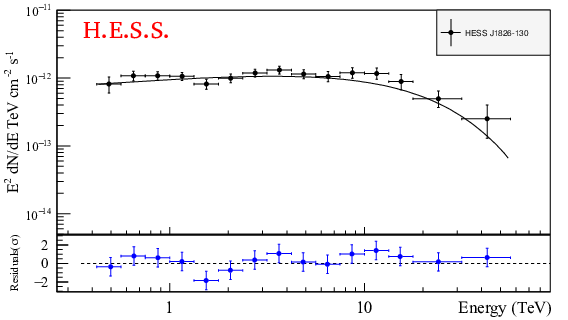
\includegraphics[height=0.18\textheight]{04_Introduction/Images/pulsar_wind_nebula/1826_energy_flux.png}
    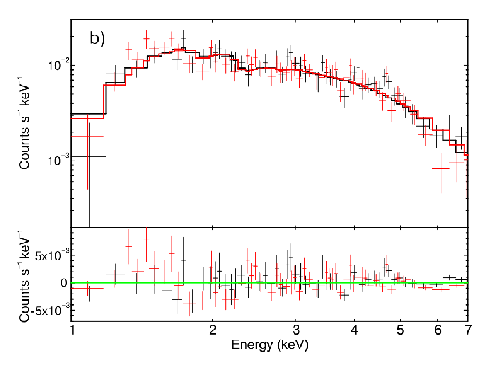
\includegraphics[height=0.18\textheight]{04_Introduction/Images/pulsar_wind_nebula/hess_j1826_130_xray.eps}
	\caption{$\TeV$ (\textit{left}) and X-ray (\textit{right}) SED towards \mbox{HESS\,J1826-130} as seen by H.E.S.S. and Suzaku respectively. Images courtesy of \cite{2020A&A...644A.112H} and \cite{2019A&A...623A.115D} respectively.}
	\label{fig:chapter1_hess_j1826_SED}
\end{figure}


\begin{table}[h!]
    \caption{Fit parameters to the spectrum of \mbox{HESS\,J1826-130}. Power law (PL): $\dv{N}{E}\propto \qty(\frac{E_p}{E_0})^{-\Gamma}$. Exponential Cutoff Power Law (ECPL): $\dv{N}{E}\propto \qty(\frac{E_p}{E_0})^{-\Gamma}\exp(-\frac{E}{E_c})$. Broken Power Law (BPL): $\dv{N}{E}\propto \qty(\frac{E_p}{E_b})^{-\Gamma}$ where $\Gamma=\Gamma_1$ if $E<E_b$ and $\Gamma=\Gamma_2$ otherwise. $E_0=1~\TeV$ unless specified.}
    \resizebox{\textwidth}{!}{
    \begin{threeparttable}
    \centering
    \begin{tabular}{rllllll}
        \toprule
        Model & $\Gamma$ & Parameters & RA & DEC & extent ($^\circ$) & References \\
        \midrule
        \textbf{HESS J1826-130} & - & - & $18\si{\hour}26\si{m}02.1\si{\second}$ & $-\ang{13}01\si{m}02.6\si{\second}$ & $0.15^*$ & a \\
        PL & $2.12\pm0.04$ & - & - & - & - & a \\
        ECPL & $1.78\pm0.10$ & $E_c = 15.2\pm5$ & - & - & - & a \\
        BPL & $1.96\pm0.06$ & $E_b = 11.2\pm2.7~\TeV$ & - & - & - & a \\
        & $3.59\pm0.69$ & - & - & - & - & - \\
        \bottomrule
    \end{tabular}
    \begin{tablenotes}
	\item \textbf{References}
	\item a: \citep{2020A&A...644A.112H}
    \end{tablenotes}
    \end{threeparttable}
    }
    \label{tab:chapter1_1826_parameters}
\end{table}

\begin{figure}[ht]
    \centering
    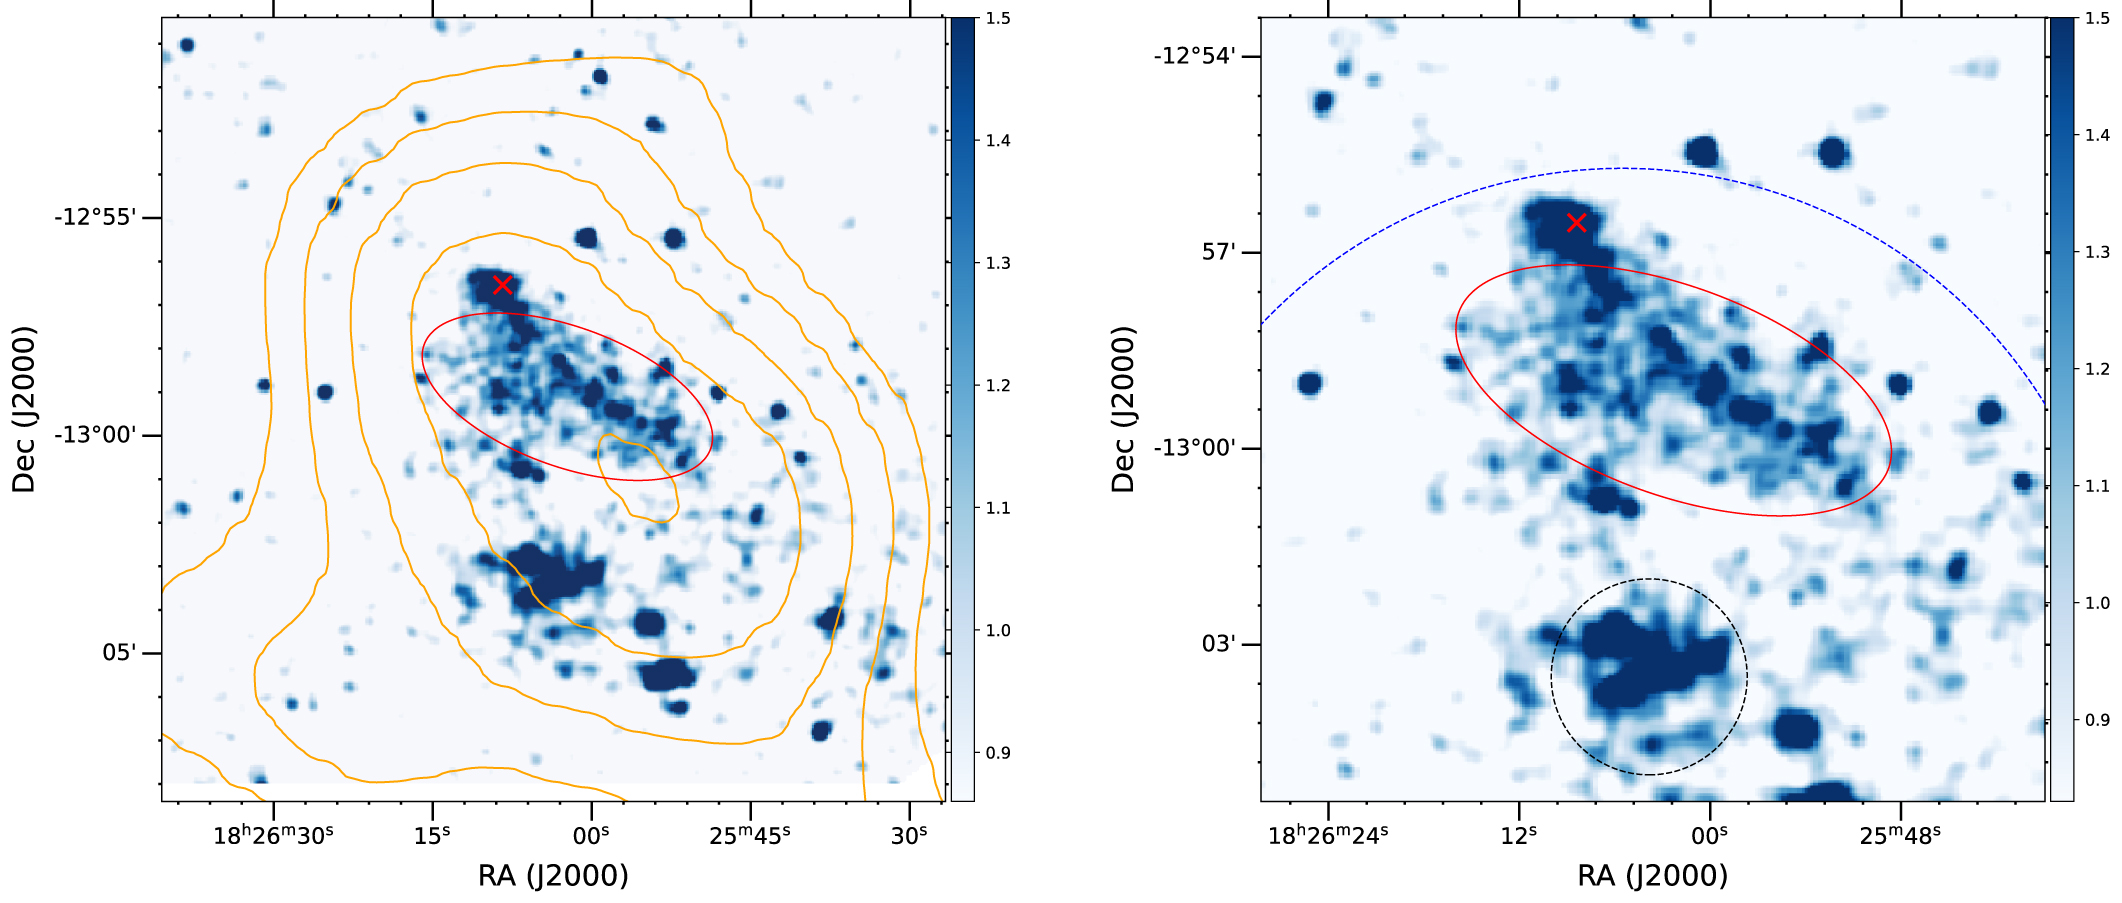
\includegraphics[width=0.9\textwidth]{04_Introduction/Images/pulsar_wind_nebula/hess_j1826_130_xray.jpg}
    \caption{XMN-Newton $0.5-10~\keV$ X-ray images towards \mbox{HESS\,J1826-130}. The positions of \mbox{PSR\,1826-1256} and the Eel Nebula are shown by the red cross and ellipse respectively. The orange lines represent the H.E.S.S. $3\sigma$ and $5\sigma$ significance contours. Nearby \mbox{SNR\,G18.45-0.42} and star cluster \mbox{Bica 3} are shown by the dashed blue and black circles respectively.  Image courtesy of \cite{2022ApJ...930..148B}.}
    \label{fig:chapter1_hess_j1826_xray}
\end{figure}

\mbox{HESS\,J1826-130}, an unidentified gamma-ray source situated $\approx\ang{0.7}$ to the Galactic north of \mbox{HESS\,J1825-137} (see \autoref{fig:chapter1_hess_j1825_137_object_positions}). Due to its proximity, \mbox{HESS\,J1826-130} was originally thought to be an extension of \mbox{HESS\,J1825-137} until it was classified as a separate source through its energy-dependent morphology \citep{2017AIPC.1792d0024A}. \mbox{HESS\,J1826-130} becomes more distinct from \mbox{HESS\,J1825-137} at higher gamma-ray energies. The analysis conducted by \cite{2020A&A...644A.112H} showed that \mbox{HESS\,J1825-137} contaminates the SED of \mbox{\mbox{HESS\,J1826-130}} by approximately $40\%$ below $1.5~\TeV$ and $20\%$ above $1.5~\TeV$. As shown by \autoref{fig:chapter1_hess_j1825_137_object_positions}, the position of \mbox{eHWC\,J1825-134} lies approximately midwway between \mbox{HESS\,J1825-137} and \mbox{HESS\,J1826-130}. Due to the coarse angular resolution of HAWC, \mbox{eHWC\,J1825-134} may represent the combined emission from both \mbox{HESS\,J1825-137} and \mbox{HESS\,J1826-130}.
\par~\par
Several objects towards \mbox{HESS\,J1826-130} have been associated with the gamma-ray emission based on spatial correlation. This includes the Eel nebula (\mbox{PWN\,G18.5-0.4}), a PWN with a long faint trail ($\ang{0.1}$) of hard X-ray emission above $2~\keV$ (see \autoref{fig:chapter1_hess_j1826_xray}) \citep{2007whsn.conf...24R,2022ApJ...930..148B}.  Similarly, \cite{2018A&A...612A...1H} proposed two possible SNRs as a source of protons interacting with the interstellar gas to produce the observed gamma-ray emission; \mbox{SNR\,G018.1-0.1} and \mbox{SNR\,G018.6-0.2.} As shown by the purple cross in \autoref{fig:chapter1_hess_j1825_137_object_positions}, \mbox{PSR\,1826-1256} is located towards \mbox{HESS\,J1826-130} and may be a source of electrons powering the PWN. \mbox{PSR\,1826-1256} has spin down power and characteristic age of $3.6\times10^{36}~\ergspersec$ and $14~\kiloyear$ respectively \citep{2010ApJS..187..460A}. %The lack of DM distance measurements to the pulsar makes it difficult to solidify its connection to the Eel nebula, \mbox{HESS\,J1826-130} and the aforementioned SNRs.
\par~\par
\cite{2016MNRAS.458.2813V} revealed dense turbulent molecular gas between \mbox{HESS\,J1825-137} and \mbox{HESS\,J1826-130}. The same study places the majority of these clouds in the $40-60~\kmpersec$ velocity range, equivalent to a distance of $3.5-4.5~\kpc$ as given by the Galactic rotation model (see \autoref{sec:06_galactic_rotation} \citep{1993A&A...275...67B}). This is consistent with the DM distance of \mbox{PSR\,J1826-1334}. Therefore, protons from the associated SNR may interact with these dense clouds through p-p collisions (see \autoref{sec:chapter1_hadronic_gr_emission}) to emit the high-energy gamma-rays as seen by \mbox{eHWC\,J1825-134}.

\section{Cosmic Rays} \label{sec:01_cosmic_rays}

As discussed in \autoref{sec:01_PWN}, PWN are a source of high-energy cosmic rays. Therefore, it is vital to understand the properties of cosmic rays in order to explain PWN characteristics.
\begin{figure}[ht]
	\centering
	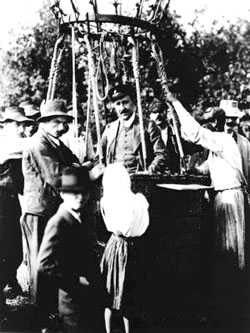
\includegraphics[width=0.7\textwidth]{04_Introduction/Images/History/hess_balloon_flight.jpg}
	\caption{Victor HESS about to ascend to an altitude $>5~\si{\kilo\meter}$ to discover cosmic rays \citep{hess1912observations}}
	\label{fig:chapter1_hess_balloon_flight}
\end{figure}
\par~\par 
In 1896 Henri Becquerel discovered that uranium salts emitted a form of invisible radiation that could could penetrate through solid matter. At the beginning of the 20th century, it was generally believed that only elements in the Earth could emit such radiation. However in 1912, Victor HESS ascended $5~\km$ with an electroscope in a hot air balloon. He noticed that as altitude increased, the amount of radiation measured by the electroscope increased \citep{hess1912observations}. In contrast, Millikan submerged electroscopes in Muir Lake located in the Rocky Mountains \citep{1926PhRv...28..851M}.  As the electroscopes descended, less radiation was detected. The findings of Hess and Millikan showed that ionising radiation, later dubbed `cosmic rays', originate from the sky. In the mid 20th century, the level of cosmic-ray ionisation was found to be dependent on latitude due to deflection by the Earth's magnetic field \citep{1960Natur.187.1099S}.
\par~\par
Cosmic rays comprise of protons, electrons, nuclei, neutrinos and anti-matter. Within this thesis, cosmic rays will be referred to as protons and electrons. Protons consist of three quarks (two up and one down-quark) and are classified as hadrons, a composite subatomic particle made of two or more quarks held together by the strong force. Meanwhile, electrons are elementary particles that belong in the lepton `family' in the standard model of particle physics. Henc, hadronic cosmic rays refer to protons while leptonic cosmic rays refer to electrons.
\par~\par 
Supernovae were proposed as a source for cosmic rays by \cite{1934PNAS...20..259B} in the 1930s. In his 1949 paper, Enrico Fermi provided a method where shock fronts (including those generated by SNRs) accelerate cosmic ray protons up to ultra-high energies \citep{1949PhRv...75.1169F}. SNRs also accelerate cosmic ray electrons up to high energies as indicated by X-ray emission produced through synchrotron interactions at the rims of SNRS such as \mbox{SN\,1006} \citep{1995Natur.378..255K}.
\par~\par
Other sources that have been proposed as accelerators of cosmic rays include PWN (as discussed in \autoref{sec:01_PWN}), star clusters, binary systems and active Galactic nuclei.

\subsection{Acceleration of Charged Particles}

\subsubsection{Acceleration by pulsars}

As discussed in \autoref{sec:01_PWN_pulsar}, pulsars are the highly dense, magnetised remnants of a supernova. The Lorentz equation,

\begin{equation}
    \begin{aligned}
        \vec{F}=q\vec{E} + q\vec{v}\times \vec{B}\text{ ,}
    \end{aligned} \label{eq:chapter_1_lorentz_force}
\end{equation}

\noindent shows that a magnetic field of strength $\vec{B}$ applies a perpendicular force, $\vec{F}$, on a particle with charge $q$. In other words, a uniform magnetic field does not change the energy of the particle. However, the rotation of a pulsar coupled with its strong magnetic field generates an electric field, $\vec{E}$. This is described by Faraday's law:
 
 \begin{equation}
    \begin{aligned}
    \nabla \times \vec{E} &= -\pdv{\vec{B}}{t}\text{ .}
    \end{aligned} \label{eq:chapter_1_maxwell_faraday_law_p1}
\end{equation}

\noindent The integral form of \autoref{eq:chapter_1_maxwell_faraday_law_p1} describes a changing magnetic field across a surface with cross sectional area  $\dd{\vec{A}}$:

\begin{equation}
    \begin{aligned}
    \oint_S \vec{E}\cdot \dd{\vec{l}}&=-\int_S \pdv{\vec{B}}{t} \cdot \dd{\vec{A}}\text{ .}
    \end{aligned} \label{eq:01_intro_alven_eq}
\end{equation}

\noindent Where the cross sectional area is the area swept up by expanding surface $S$ in segment $\dd{\vec{\ell}}$ and velocity $\vec{v}$ over time $\dd{t}$ ($\dd{\vec{A}}=\dd{\vec{\ell}}\times \vec{v}\dd{t}$). \autoref{eq:01_intro_alven_eq} becomes: 

\begin{equation}
    \begin{aligned}
    \oint_S \vec{E}\cdot \dd{\vec{l}}&=\int_S \vec{v}\times \vec{B}\cdot \dd{\vec{\ell}}\text{ .}
    \end{aligned} \label{eq:chapter_1_maxwell_faraday_law_p2}
\end{equation}

\noindent i.e. the electric field generated by the pulsar is proportional to the rotation and magnetic field of the pulsar. 
\par~\par 
The change in energy, $\mathcal{E}$, of particles in the presence of an electric field is given by:

\begin{equation}
    \begin{aligned}
    \dv{\mathcal{E}}{t}&=\dv{}{t} \qty(\half m\vec{v}^2) = m \vec{v} \cdot \dv{\vec{v}}{t} = \vec{v} \cdot \vec{F} = q\vec{v} \cdot \vec{E}\text{ .}
    \end{aligned} \label{eq:chapter_1_gain_energy_fields}
\end{equation}
\noindent Therefore, the electric field generated by the pulsar strips particles from its surface and accelerates them up to high energies. The maximum electric field strength produced by a fluctuating magnetic field is described by $E_\text{max}=v_\text{plasma}B$, giving the maximum energy gain rate:
\begin{equation}
    \begin{aligned}
    \dv{\mathcal{E}}{t}_\text{max}&=qv^2B\text{ .}
    \end{aligned}
\end{equation}
\noindent For relativistic particles:

\begin{equation}
    \begin{aligned}
    \dv{\mathcal{E}}{t}_\text{acc}=\zeta Zec^2B\text{ ,}
    \end{aligned}
\end{equation}
where $0<\zeta<1$ is an "acceleration rate parameter" that depends on the acceleration mechanism and $Z$ is the charge of the particle \citep{2022arXiv221116020T}. Naively, taking the surface magnetic field strength of $B=10^{11}~\si{G}$, pulsar radius of $10~\km$ and the average period of $P=0.8\,\si{\second}$ \citep{2005AJ....129.1993M}, the maximum energy gain rate of particles is $\approx 10^{17}~\si{\electronvolt\per\second}$. Simply, it would take $10^{-5}~\si{\second}$ for a pulsar to accelerate an electron/proton up to $1~\TeV$. This assumes that the particle does not escape the pulsar and suffers no energy losses.

\subsubsection{Acceleration by the pulsar wind nebula termination shock}

A termination shock forms where the internal pressure of the PWN counteracts the ram pressure of the interstellar wind at approximately $r_\text{ts}=0.1~\pc$ (see \autoref{sec:01_intro_time_ev_PWN}). Particles can be accelerated by the TS through diffusive shock acceleration (DSA) where a particle can scatter back and forth a shock due to magnetic field irregularities, resulting in an overall gain of energy (see \autoref{A3_DSA}).
\par~\par
The magnetic field of the PWNe is toroidal in nature where the magnetic field lines are perpendicular to the propagation of the shock. For a pulsar injecting electrons/positrons, the structure of the shock depends on the ratio, $\sigma$, of the upstream magnetic energy and plasma energy \citep{1992ApJ...391...73G}:

\begin{equation}
    \begin{aligned}
        \sigma&=\frac{B^2/4\pi}{nm\gamma c^2}\text{ ,}
    \end{aligned}
\end{equation}
\noindent where $B$ and $n$ is the upstream magnetic field and electron energy density respectively and $\gamma$ is the Lorentz factor of the electrons. Models of PWN suggest that the magnetization parameter takes values $10^{-3}-10^{-2}$ \citep{1974MNRAS.167....1R,1984ApJ...283..694K,2004MNRAS.349..779K}. The magnetic field turbulence is too weak for particles to scatter back and forth across the termination shock and DSA is suppressed \citep{2010MNRAS.402..321L,2015SSRv..191..519S}. In general, DSA for magnetic fields perpendicular to the shock propagation is too suppressed to accelerate electrons up the energies required to explain PWN emission \citep{2003APh....19..649M, 2014ApJ...783...91C}.
\par~\par
It has been suggested pre-acceleration of particles driven by magnetic reconnection at the shock front \citep{2001ApJ...547..437L,2003MNRAS.345..153L,2016JPlPh..82d6301L}, or resonant cyclotron absorption of electrons/positrons \cite{2001ApJ...547..437L}  followed by DSA may overcome these issues.
\par~\par
Any modelling conducted in this thesis will assume an injection of accelerated electrons.

\subsection{Propagation of charged particles} \label{chapter_1_cr_propagation}

Neglecting any electric fields, the Lorentz equation (\autoref{eq:chapter_1_lorentz_force}) shows that the magnetic force applied to a charged particle is perpendicular to its motion and the particle will travel in a circular motion described by:

\begin{equation}
    \begin{aligned}
    \vec{F}&=\frac{mv_\perp^2}{r^2}\hat{r}\text{ ,}
    \end{aligned} \label{eq:chapter_1_centripetal_motion}
\end{equation}
\begin{figure}[b!]
    \centering
    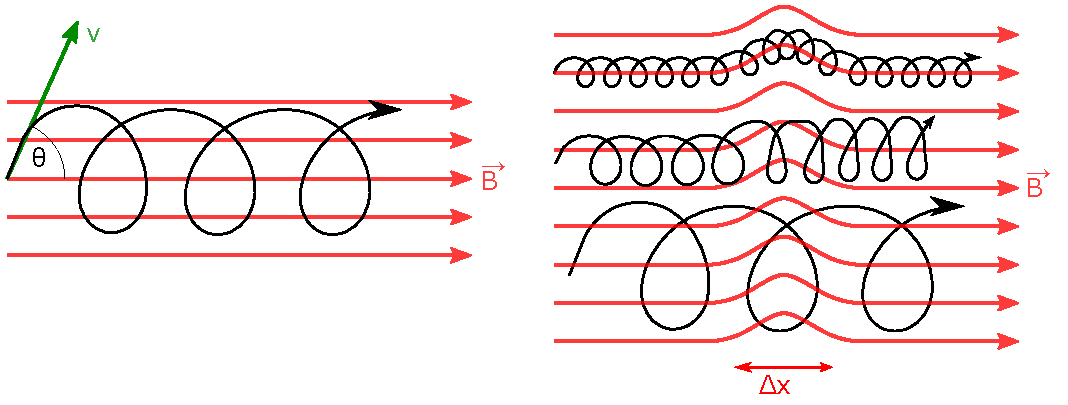
\includegraphics[width=1.0\textwidth]{04_Introduction/Images/cosmic_rays/combined_turbulence.pdf}
    \caption{ (\textit{left}) The path (black) of motion taken by a charged particle with initial velocity $v$ at angle $\theta$ to a uniform magnetic field $B$ (red). (\textit{right}) Propagation of a charged particle in a magnetic field  with turbulence of length $\Delta x$ when $r_g<\Delta x$ (\textit{top}), $r_g\approx \Delta x$ (\textit{middle}) and $r_g>\Delta x$. (\textit{bottom})}
    \label{fig:01_CR_in_Bfield}
\end{figure}

\noindent where $v_\perp$ is the velocity perpendicular to the magnetic field and $\hat{r}$ represents the direction perpendicular both to the motion and the magnetic field. Combining \autoref{eq:chapter_1_lorentz_force} and \autoref{eq:chapter_1_centripetal_motion}, we find the particle gyroradius, $r_g$ (the radius of the circular motion induced by a uniform magnetic field):

\begin{equation}
    \begin{aligned}
    r_g&=\frac{mv_\perp}{qB}=\frac{p}{qB}\text{ ,}
    \end{aligned} \label{eq:chapter_1_gyroradius}
\end{equation}
\noindent where $p$ is the momentum of the charged particle. For relativistic cosmic rays $p\approx E/c$. If the charged particle has velocity at an angle $\theta$ to a magnetic field, it will spiral around the magnetic field direction as shown in the left panel of \autoref{fig:01_CR_in_Bfield}.
\par~\par 
The magnetic field around PWNe and within dense gas clouds (see \autoref{eq:sec_Bfield_gas}) is not uniform and will affect the propagation of charged particles. The presence of magnetic field turbulence of length $\Delta x$ in an otherwise uniform field will affect the propagation of charged particles (see the right panel of \autoref{fig:01_CR_in_Bfield}). For charged particles, where the gyroradius is much less than the magnetic turbulence ($r_g\ll \Delta x$), the particle will follow the magnetic field lines with no changed to its pitch angle. When the gyroradius is much greater than the turbulence ($r_g\gg \Delta x$), the propagation will be unaffected. For charged particles, where the the gyroradius is similar in scale to the perturbation ($r_g\approx \Delta x$), the pitch angle $\theta$ changes and alters the direction of travel. In other words, charged particles scatter on the magnetic field turbulence that is of similar scale as the gyroradius.
\par~\par
The gyroradius of ultra-high energy particles ($r_g=3.6~\kpc$ at $10^{19}~\eV$ and $B=3~\si{\micro G}$) is so large that they tend to travel in a ballistic manner (for distances less than $r_g$) and thus point back to their place of origin. Lower energy particles (e.g. $r_g\approx 10^{-4}~\pc$ at $1~\TeV$ and $B=3~\si{\micro G}$) scatter multiple times and their trajectory tends to follow a random walk, i.e. diffusion.

\subsubsection{Diffusion of charged particles} 

The diffusion coefficient, $D~\qty[\si{\centi\meter\squared\per\second}]$, describes the rate that charged particles diffuse per unit area of time and is related to the magnetic field of the medium. In a magnetic field with average field strength $B_0$, the mean square variation $\delta B^2$ depends on the spatial power spectrum of the magnetic field turbulence $I\qty(k)\propto k^{-\Gamma}$ \citep{1983RPPh...46..973D,2016MNRAS.461.3552N}:

\begin{equation}
    \begin{aligned}
        \int I\qty(k) \dd{\ln k}&= \qty(\frac{\delta B}{B_0})^2\text{ ,}
    \end{aligned}
\end{equation}
\noindent where $k\propto 1/r_g$ is the wave number. As the charged particle spirals around the magnetic field lines (see \autoref{fig:01_CR_in_Bfield}), the pitch angle of the particle is changed by order $\delta B$. The pitch angle is randomised after approximately $N=B_0^2/kI\qty(k)$ rotations such that the mean free path parallel to the field is given by $\lambda_\parallel=Nr_g$. Therefore the diffusion coefficient parallel to the magnetic field lines:

\begin{equation}
    \begin{aligned}
        D_\parallel&=\frac{r_gv}{3}\frac{B_0^2}{kI\qty(k)}\text{ ,}
    \end{aligned} \label{eq:01_diff_parallel}
\end{equation}
\noindent where $v$ is the velocity of the particle. The mean free path perpendicular to the field lines takes values $\lambda_\perp\approx r_g$ such that the perpendicular diffusion coefficient becomes:

\begin{equation}
    \begin{aligned}
        D_\perp&=\frac{r_gv}{3}\frac{kI\qty(k)}{B_0^2}=D_\parallel\qty(\frac{kI\qty(k)}{B_0^2})^2\text{ .}
    \end{aligned}
\end{equation}
\noindent Hence:

\begin{equation}
    \begin{aligned}
        D_\perp D_\parallel&=\qty(\frac{r_gv}{3})^2=D_B^2\text{ ,}
    \end{aligned}
\end{equation}
\noindent where $D_B=r_gv/3$ is known as the Bohm diffusion coefficient representing the case when $\lambda\approx r_g$.
\par~\par 
Three different regimes of turbulence are considered: Bohm ($\Gamma=1$), Kraichnan ($\Gamma=\frac{3}{2}$) and Kolomogrov ($\Gamma=\frac{5}{3}$). Quasi-linear theory states that diffusion perpendicular to the magnetic field lines is negligible (\cite{2016MNRAS.461.3552N} and references within). As $r_g\propto E$ and $k\propto 1/E$, \autoref{eq:01_diff_parallel} becomes:

\begin{equation}
    \begin{aligned}
        D&\propto \frac{r_g}{kI\qty(k)}\propto E^{2-\Gamma} \text{ .}
    \end{aligned}
\end{equation}
This results in energy dependent diffusion: $D\propto E$ in the Bohm regime, $D\propto E^{\frac{1}{2}}$ in the Kraichnan regime and $D\propto E^{\frac{1}{3}}$ in the Kolmogrov regime. From cosmic-ray observations, values of the diffusion coefficient follows a power law spectrum ($D\propto E^{\delta}$) with $\delta$ taking values between $0.3-0.6$, implying a situation in the Kraichnan/Komogrov regime (e.g. see \cite{2007ARNPS..57..285S}).
\par~\par 
Neglecting acceleration, \cite{2007Ap&SS.309..365G} parameterized the diffusion coefficient for cosmic rays of energy $E$ travelling in a molecular cloud with a magnetic field $B$ to be:
\begin{align}
    D\qty(E,B)&=\chi D_0\qty(\frac{E/\GeV}{B/3~\si{\micro G}})^\delta\quad [\si{\centi\meter\squared\per\second}] \label{eq:diffusion}
\end{align}
where $D_0=1\times 10^{27}~\si{\centi\meter\squared\per\second}$ is the Galactic diffusion coefficient at $1~\GeV$ and the factor, $\chi$, takes values\,$<1$ and accounts for the suppression of the diffusion coefficient inside turbulent clouds \citep{1990acr..book.....B}. \cite{1996A&A...309..917A} consider $\chi=0.01$ to be `slow' diffusion representing dense ISM clouds \citep{1988ApJ...334..722O} and $\chi=1$ to be `fast' diffusion. The diffusion suppression factor is poorly constrained but studies towards SNR W28: \citep{2010MNRAS.409L..35L}, \citep{2010A&A...516L..11G} and \cite{2010sf2a.conf..313G} assume $\chi=0.1$, $0.01$ and $0.06$ respectively for $D_0=10^{28}~\si{\centi\meter\squared\per\second}$ at cosmic ray energy $10~\GeV$. Similarly, \cite{2008MNRAS.390..683P} highlighted the variation of the suppression factor ($\chi=0.01$, $0.1$, $1$ and $\chi \gg 1$) in studies towards star forming region Sgr\,B2.

\subsubsection{Local and Galactic Magnetic Fields}

Magnetic fields affect the propagation of charged particles through the Galaxy. Faraday rotation (the rotation of polarised light in magnetised plasma) can be used to measure the magnetic field strength in the Galaxy \citep{1846RSPT..136....1F}:

\begin{equation}
    \begin{aligned}
    \langle B_\parallel \rangle = 1.232 \frac{\text{RM}}{\text{DM}}\text{ ,}
    \end{aligned}
\end{equation}
\noindent where $B_\parallel$ is the magnetic field component along the line of sight, RM is the rotation measure due to Faraday rotation and DM (see \autoref{eq:chapter_1_dispersion_measurement} is the dispersion measurement of the pulsar. Magnetic fields are also measured through observations of synchrotron emission, where the intensity is proportional to the magnetic field strength and electron energy density (see \cite{2013pss5.book..641B} and references within).
\par~\par 
The magnetic field in the `local' vicinity takes value $1-6~\si{\micro G}$ based on both rotation measure and synchrotron measurements  \citep{1989ApJ...343..760R,2001SSRv...99..243B}.  Using the rotation measures from $223$ pulsars, \cite{2006ApJ...642..868H} found the magnetic field strength in the Galactic disk was found to depend on the distance to the Galactic centre:

\begin{equation}
    \begin{aligned}
        B=B_0\exp[-\frac{R-R\odot}{R_B }]\text{ ,}
    \end{aligned}
\end{equation}
where $B_0=2.1\pm 0.3~\si{\micro G}$ and $R_B=8.5\pm 4.7~\kpc$. This gives the average Galactic magnetic field to be approximately $ 3~\si{\micro G}$. Local sources such as PWN (see \autoref{sec:01_PWN}), SNRs (see \citep{2012SSRv..166..231R} and references within) and turbulent molecular clouds \citep{2010ApJ...725..466C} provide an `additional' magnetic field component to their surrounding environment.

\subsection{Cosmic Ray Spectrum} \label{sec:chapter_1_cr_spectrum}
\begin{SCfigure}[0.4][h!]
    \centering
    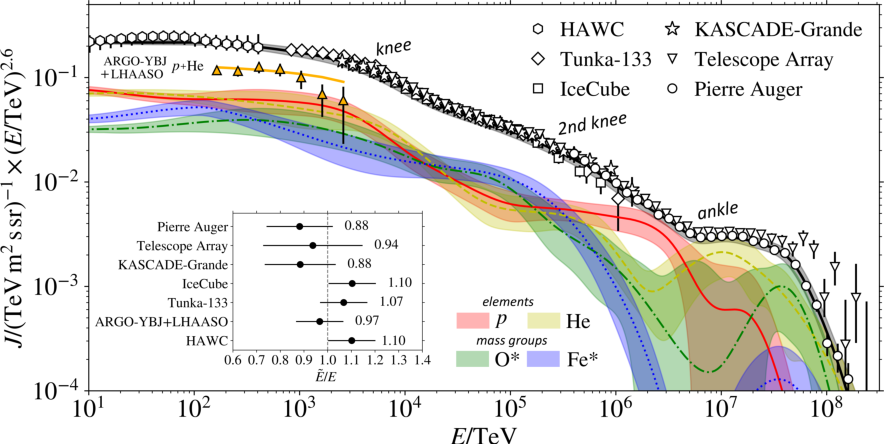
\includegraphics[width=0.75\textwidth]{04_Introduction/Images/cosmic_rays/cosmic_ray_spectrum.pdf}
    \caption{Cosmic ray (and high-energy electrons) energy spectrum at Earth as measured by multiple ground-based observatories. Image courtesy of \cite{2019BAAS...51c.131S}}
    \label{fig:chapter1_cosmic_ray_flux}
\end{SCfigure}
\par~\par
The energy spectrum of cosmic rays (see \autoref{fig:chapter1_cosmic_ray_flux}) has been measured up to $10^{20}~\eV$ \citep{2022arXiv221116020T} and broadly follows a power-law:

\begin{equation}
    \begin{aligned}
    \dv{N}{E}&\propto E^{-\Gamma}\text{ .}
    \end{aligned}
\end{equation}

Below $10~\GeV$, the cosmic ray energy spectrum is dominantly composed of high-energy particles originating from the Sun. Below this energy, there are few cosmic rays that originate from outside the solar system due to "frozen in" magnetic fields carried by the solar wind. Cosmic rays below $10~\GeV$ have a gyro-radius (see \autoref{eq:chapter_1_gyroradius}) smaller than the magnetic irregularities within this structure and are scatted out of the solar system \citep{2002cra..book.....S}. The cosmic ray spectrum broadly follows a power law with spectral index $\Gamma\approx 2.7$ until the `knee' at $10^{15}~\eV=1~\PeV$ when it steepens to an index of $3$. Ground-based cosmic ray detectors have reported a second knee at $10^{17}~\eV$ where the spectrum steepens further to $3.3$ until it flattens out to $\approx 2.6$ at the ankle ($10^{18}~\eV=1~\si{E\electronvolt}$) \citep{2008ApJ...678.1165A,2010PhLB..685..239A, 2013PhRvD..87h1101A, 2013PhRvD..88d2004A,2013ApJ...768L...1A}. The knee and ankle feature is believed to be created due to the transition of Galactic cosmic-rays (from sources such as SNRs and PWNe) to extra-Galactic cosmic rays possibly originating from AGN \citep{2016A&A...595A..33T}. The cosmic ray spectrum then experiences a sharp cutoff at $29\times10^{18}~\eV = 29~\si{E\electronvolt}$ due to the GKZ cutoff, where cosmic ray protons and nuclei interact with the the CMB and rapidly lose their energy \citep{1966PhRvL..16..748G,1966JETPL...4...78Z}. 

\subsection{PeVatrons} \label{sec:chapter_1_PeVatrons}
\begin{table}[h!]
    \caption{Observed HAWC and LHAASO sources with significant gamma-ray emission greater than $100~\TeV$
    \citep{PhysRevLett.124.021102,2021Natur.594...33C}. The sources equivalent to \mbox{HESS\,J1825-137} are highlighted in blue.}
    \label{tab:chapter1_peVatron_candidates}
    \resizebox{\textwidth}{!}{
    \begin{threeparttable}
    \centering
   \begin{tabular}{ccccc}
        \hline
         & \textbf{Source} & \textbf{$\TeV$ counterpart$^*$} & \textbf{Accelerator$^*$} & $\sqrt{\text{TS}}$ \\
         \hline
         \textbf{HAWC} &  & & & \\
         & \textcolor{blue}{eHWC\,J1825-134} & \textcolor{blue}{\mbox{HESS\,J1825-137}, \mbox{HESS\,J1826-130}} & \textcolor{blue}{PWN} & \textcolor{blue}{$41.1$} \\
         & eHWC\,J1907+063 & HESS J1908+063 & Unidentified & $37.8$ \\
         & eHWC\,J2019+368 & 2HWC J2019+367 & Possible PWN$^{a}$ & $32.2$ \\
         \textbf{LHAASO} & & & & \textbf{Significance} \\
         & & & & $>100~\TeV (\times \sigma)$ \\
         & LHAASO J0534+2202 & Crab Nebula & PWN & $17.8$ \\
         & \textcolor{blue}{LHAASO J1825-1326} & \textcolor{blue}{HESS J1825-137} & \textcolor{blue}{PWN} & \textcolor{blue}{$16.4$} \\
         & LHAASO J1839-0545 & HESS J1837-069 & Possible PWN & $7.7$ \\
         & LHAASO J1843-0338 & HESS J1843-033, HESS J1844-030, & Possible SNR & $8.5$ \\
         & & SNR G28.6-0.1 & & \\
         & LHAASO J1849-0003 & HESS J1849-000, W43W  & Possible PWN$^{b}$ & $10.4$ \\
         & LHAASO J1908+0621 & HESS J1908+063, MGRO J1908+06 & Possible SNR or PWN & $17.2$ \\
         & LHAASO J1929+1745 & HESS J1930+188 & Possible PWN or SNR & $7.4$ \\
         & LHAASO J1956+2845 & 2HWC J1955+285, SNR G66.0-0.0 & Possible PWN SNR & $7.4$ \\
         & LHAASO J2018+3651 & MGRO J2019+37  & Possible PWN & $10.4$ \\
         & LHAASO J2032+4102 & - & Possible PWN & $10.5$ \\
         & LHAASO J2108+5157 & - & Possible PWN & $8.3$ \\
         & LHAASO J2226+6057 & Boomerang Nebula & Possible SNR or PWN & $13.6$ \\
         \hline
    \end{tabular}
    \begin{tablenotes}
	\item $^*$: Counterparts are based on spatial correlation.  \\
	\textbf{References}
	\item $^{a}$ \cite{2018APS..APRB17003B} 
	\item $^{b}$ \cite{2015MNRAS.449.3827K} 
    \end{tablenotes}
    \end{threeparttable}
    }
\end{table}
The transition from Galactic to extra-Galactic cosmic rays in the cosmic ray spectrum occurs between $10^{15}~\eV$ and $10^{18}~\eV$ with Galactic cosmic rays expected to contribute up to $10^{17}~\eV=100~\PeV$ \citep{2016A&A...595A..33T}. Sources capable of accelerating particles up to and beyond $1~\PeV=10^{15}~\eV$ are known as PeVatrons. Finding Galactic PeVatrons are key to understanding the mechanism of accelerating particles up to $\PeV$ energies.
\par~\par
Cosmic rays with energies $1~\PeV$ and $100~\PeV$ have gyroradii of $\approx 0.4~\pc$ and $40~\pc$ respectively, making their direct origin impossible to determine. However, cosmic rays interact with interstellar gas and magnetic fields near their birthplace to produce gamma rays with energies greater than $100~\TeV$ (see \autoref{sec:chapter1_non_thermal_emission}). Therefore, any gamma-ray source with significant gamma-ray emission above $100~\TeV$ is an indicator of a PeVatron
\par~\par 
The High-Altitude Water Cherenkov Gamma-ray observatory (HAWC) and the Large High Altitude Air Shower observatory (LHAASO) are observatories that detect the air shower triggered by gamma rays \citep{LHAASO_website, HAWC}. \autoref{tab:chapter1_peVatron_candidates} lists observed HAWC and LHAASO sources with significant gamma-ray emission above $100~\TeV$ with possible counterparts and accelerator type \citep{PhysRevLett.124.021102,2021Natur.594...33C}. In the past, SNRs have been regarded as the most likely source capable of accelerating protons up to $\PeV$ energies. However, there has been no firm identification of a SNR PeVatron and their suitability as a PeVatron has been called into question \citep{10.1093/mnras/sty1589,2019IJMPD..2830022G,2021Univ....7..324C,2022MNRAS.516..492B}. However, both the Crab Nebula and \mbox{HESS\,J1825-137} are confirmed $\TeV$ PWN counterparts of \mbox{LHAASO\,J0534+2202} and \mbox{LHAASO\,J1825-1326} respectively. Out of the remaining LHAASO candidates, at least eight have possible PWN counterparts. PWN are now being considered as possible candidates to accelerate electrons up to $\PeV$ energies \citep{2021ApJ...908L..49B,de_O_a_Wilhelmi_2022}. \cite{2022ApJ...928...19V} suggests that unresolved PWNe provides significant contribution to the diffuse gamma-ray emission above $100~\TeV$.
\par~\par
H.E.S.S. has only discovered one PeVatron that is postulated to be associated with the Galactic Center during an active phase \cite{2016Natur.531..476H}. They highlighted that the current rate of particle acceleration is not powerful enough to explain the cosmic-ray flux at Earth.  Alternatively, superbubbles and massive stellar clusters have been proposed as PeVatron candidates. Stellar clusters form within dense molecular clouds, creating an expanding `bubble' of low density ISM \citep{1998LNP...506..399I}. It has been suggested that turbulent plasma within superbubbles confine cosmic rays, allowing multiple shock fronts to accelerate them to high energies (e.g. see \cite{2022MNRAS.515.2256V} and references within).
\par~\par 
The \mbox{Tibet AS$\gamma$} collaboration revealed the detection of diffuse gamma rays with energies between $100~\TeV$ to $10^3~\TeV=1~\PeV$ in the Galactic disk, indicating the presence of PeVatrons in the Galaxy \citep{PhysRevLett.126.141101}. Similarly, LHAASO reported measurements of the diffusive gamma-ray emission up to $1000~\PeV$ and suggests that $\TeV$ halos (see \autoref{sec:01_intro_time_ev_PWN}) significantly contribute to the diffusive emission up to the ultra-high energy band \citep{2023arXiv230505372C}.

\section{Gamma-rays: messengers of cosmic rays} \label
{sec:chapter1_non_thermal_emission}
\autoref{chapter_1_cr_propagation} and \autoref{sec:chapter_1_PeVatrons} discussed how Galactic cosmic rays ($E<100~\PeV$) scatter off magnetic field turbulence, thus do not preserve information about their origin. Therefore, alternate messengers for Galactic cosmic rays must be turned to. Gamma-rays are produced via hadronic (cosmic ray proton) and leptonic (cosmic ray electron) interactions with the ISM and/or radiation fields. This section will describe the history of gamma-ray astronomy and then delve deeper into their production processes.

\subsection{A brief history}

Gamma rays were first discovered in 1900 by Paul Villard while studying radium. Ernest Rutherford later realised in 1903 that this radiation was fundamentally different to alpha, beta and delta-rays and subsequently classified them as gamma rays. By reflecting gamma-rays from a crystal surface, Rutherford and Edward Andrade in 1913 proved the electromagnetic nature of gamma-rays and measured their wavelength \citep{1913Natur..92..267R}. Gamma-rays have the largest energy per photon and smallest frequency of the electromagnetic spectrum. On Earth, gamma rays are created by radioactive decay within the crust and the interaction of cosmic rays with the Earth's atmosphere. Gamma-ray astronomy began with the 1957 publication by Philip Morrison, with the prediction that solar flares produce gamma-rays \citep{1958NCim....7..858M}. We now know of many astrophysical sources that can produce gamma-rays. These include PWNe, SNRs, quasars and active Galactic nuclei. Current gamma-ray observatories include \textit{Fermi} Gamma-ray Space Telescope \citep{nasa_fermi_site}, the High Energy Stereoscopic System \citep{HESS}, MAGIC \citep{MAGIC}, HAWC \citep{HAWC}, VERITAS \citep{VERITAS} and LHAASO \citep{LHAASO_website}. Details of gamma-ray detection will be discussed in \autoref{sec:02_astronomy}.

\subsection{Hadronic Gamma-Ray Emission} \label{sec:chapter1_hadronic_gr_emission}

Relativistic protons (and nuclei) can collide with gas in the ISM to form charged and neutral pions via proton-proton (p-p) interactions:

\begin{equation}
    \begin{aligned}
    p+p&\rightarrow \pionneutral + \pionplus + \pionminus
    \end{aligned}
\end{equation}
\noindent During p-p interactions, about half of the energy of the initial cosmic-ray proton is split among the neutral and charged pions  \citep{2009ARA&A..47..523H}. The subsequent decay of the neutral pions produces gamma rays as per:

\begin{equation}
    \begin{aligned}
    \pionneutral & \rightarrow \gamma +\gamma
    \end{aligned}
\end{equation}
\noindent with each gamma ray carrying approximately one sixth of the initial proton energy \citep{2009ARA&A..47..523H}. The charged pions decay into muons, neutrinos and anti-neutrinos:

\begin{equation}
    \begin{aligned}
    \pionplus &\rightarrow \muonplus + \muonneutrino \\
    \pionminus &\rightarrow \muonminus + \antimuonneutrino
    \end{aligned}
\end{equation}
\noindent Similarly, muons go on to decay into electrons, positions, neutrinos and anti-neutrinos:

\begin{equation}
    \begin{aligned}
    \muonminus &\rightarrow e^- + \bar{\nu}_e+\nu_\mu \\
    \muonplus &\rightarrow e^+ + \nu_e + \bar{\nu}_\mu
    \end{aligned}
\end{equation}
\begin{figure}[h!]
    \centering
    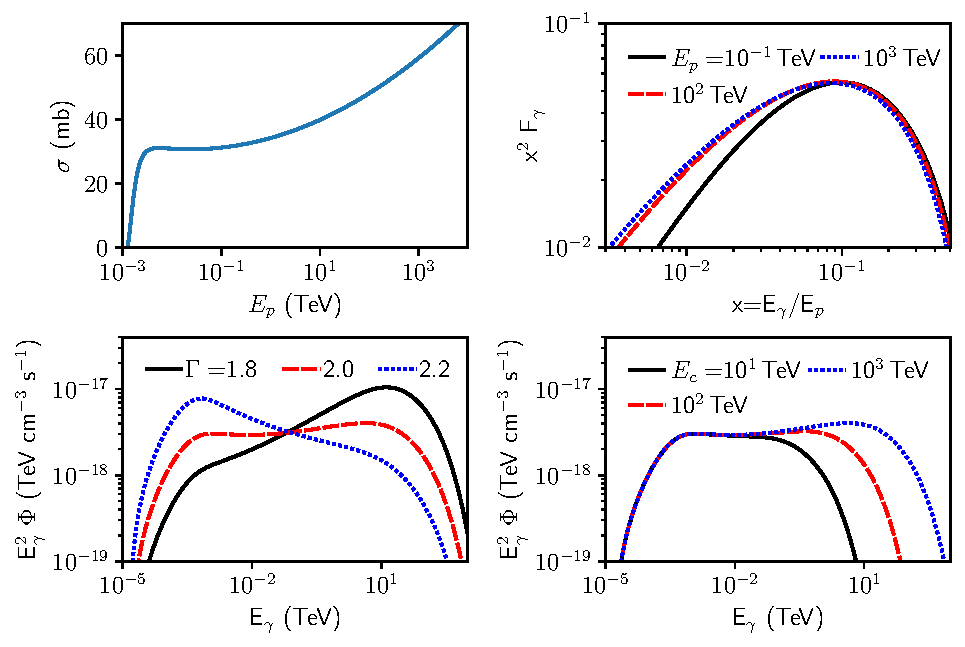
\includegraphics[width=\textwidth]{04_Introduction/Images/non_thermal_emission/hadronic_interaction.pdf}
    \caption{(\textit{top-left}) Proton-proton interaction cross section as given by \autoref{eq:chapter1_non_thermal_pp_cross_section}. (\textit{top-right}) Hadronic gamma-ray emission from a cosmic-ray proton with energy $E_p$ and target density $n_H=1~\centimeterminusthree$ (\textit{bottom}) Gamma-ray spectra from p-p interactions from cosmic rays protons with an exponential cutoff power law distribution ($\dd{N}/\dd{E}\propto E^{-\Gamma}\exp(-E/E_c)$) with $E_c=10^3~\TeV$ (\textit{left}) and $\Gamma=2.0$ (\textit{right}).}
    \label{fig:chapter_1_non_thermal_hadronic_emission}
\end{figure}
\par~\par
For a distribution of protons with spectral index $\Gamma$ and exponential cutoff energy $E_c$:

\begin{equation}
    \begin{aligned}
    J_P\qty(E_p) &= A E_p^{-\Gamma} \exp(-\frac{E_p}{E_C})\quad\qty[\si{\per\tera\electronvolt\per\centi\meter\cubed}]\text{ ,}
    \end{aligned}
\end{equation}
\noindent where $A$ is a normalisation constant, the energy spectra of gamma-rays from proton-proton collisions is expected to follow:

\begin{equation}
    \begin{aligned}
	\Phi\qty(E_\gamma)&=\dv{N_\gamma}{E_\gamma}=cn_H\int_{E_\gamma}^\infty\sigma_{pp}\qty(E_p)J_p\qty(E_p)F_\gamma\qty(T_p,E_\gamma)\frac{\dd{E_p}}{E_p}\text{ ,}
\end{aligned} \label{eq:01_hadronic_g_spectrum}
\end{equation}
\noindent where $c$ is the speed of light and $n_H$ is the density of the ambient medium.
From the bottom panels in \autoref{fig:chapter_1_non_thermal_hadronic_emission} it can be seen that the shape of the p-p gamma-ray SED is influenced by the distribution of cosmic ray protons. While the spatial morphology of hadronic gamma-rays is shaped by interstellar gas, as seen in \autoref{eq:01_hadronic_g_spectrum}. In summary, gamma rays act as messengers for hadronic cosmic-rays and carry information about the source and its surrounding environment.
\par~\par
The total inelastic cross section of p-p interactions for a proton of kinetic energy $T_p$ (where the total energy is $E_p=m_pc^2+T_p$) is given by \citep{2014PhRvD..90l3014K}:

\begin{equation}
    \begin{aligned}
    \sigma_{pp}\qty(T_p) &= \qty(30.7-0.96\ln\qty(\frac{T_p}{T_\text{thr}})+0.18\ln^2\qty(\frac{T_p}{T_\text{thr}}))\qty(1-\qty(T_\text{thr}/T_p)^{1.9})^3\quad\qty[\si{\milli\barn}]\text{ ,}
    \end{aligned} \label{eq:chapter1_non_thermal_pp_cross_section}
\end{equation}
\noindent where $T_\text{thr}=2m_\pi + m_\pi^2/2m_p \approx 0.28~\GeV$ is the minimum proton kinetic energy to form a neutral pion ($E_\text{thr}=1.22~\GeV$). The top-left panel of \autoref{fig:chapter_1_non_thermal_hadronic_emission} shows the total inelastic cross section at different proton energies.
\par~\par
The time it takes for a proton to lose its energy (or `cool' to a lower energy) through p-p interactions in a medium with ambient density $n_H$ is given by \citep{2009ARA&A..47..523H}:

\begin{equation}
    \begin{aligned}
	\tau_{pp} &= \frac{1}{nc\kappa\sigma_{pp}\qty(E)} \\
	&\approx 5.3\times 10^7\qty(n/\centimeterminusthree)^{-1}\quad\qty[\si{yr}]\text{ .}
\end{aligned} \label{eq:chapter_1_pp_cooling time}
\end{equation}
\noindent \autoref{eq:chapter_1_pp_cooling time} shows that the cooling rate of protons is inversely proportional to the density of interstellar gas and approximately independent of the proton energy. Therefore, the brightness of gamma-rays towards a source of cosmic ray protons will correlate with the density morphology of the surrounding ISM gas.
\par~\par 
Using GEANT4 models, \cite{2014PhRvD..90l3014K} parameterized the spectra of gamma-rays of energy ($E_\gamma$) from a single proton with kinetic energy $T_p$ to be:

\begin{equation}
    \begin{aligned}
        F_\gamma\qty(T_p, E_\gamma)&= A_\text{max}\qty(T_p) F\qty(T_p, E_\gamma) \text{ ,}
    \end{aligned} \label{eq:chapter_1_non_thermal_hadronic_flux_single_proton}
\end{equation}
\noindent where $A_\text{max}$ is a function of the pion production and $F\qty(T_p, E_\gamma)$ describes the shape of the spectrum:

\begin{subequations}
	\begin{alignat}{2}
		A_\text{max}\qty(T_p) &=\sigma_\pi\qty(T_p)
        \begin{cases}
        {b_0}/{E_\pi^\text{max}}&\text{, } T_\text{thr}\leq T_p < 1~\GeV \\
        {b_1\theta_p^{-b_2}}/{m_p}\times \exp(b_3\ln^2\theta_p) &\text{, } T_p \geq 1~\GeV \\
        \end{cases} \\
        F_\gamma \qty(T_p, E_\gamma)&=\frac{\qty(1-X_\gamma^{\alpha\qty(T_p)})^{\beta\qty(T_p)}}{\qty(1+X_\gamma/C)^{\gamma\qty(T_p)}}\text{ ,}
	\end{alignat}
\end{subequations}
\noindent with $\sigma_\pi$ being the $\pi_0$ production cross section (see \cite{2014PhRvD..90l3014K} for parameterisation), $\theta_p=T_p/m_p$, $E_\pi^\text{max}$ is the maximum total $\pi_0$ energy in the laboratory frame, $C=\lambda  m_\pi/Y_\gamma^\text{max}$, $Y_\gamma=E_\gamma+m_\pi^2/\qty(4E_\gamma)$, $X_\gamma=(Y_\gamma-m_\pi)/(Y_\gamma^\text{max}-m_\pi)$ and $b_0=5.9$, $b_1$, $b_2$, $b_3$, $\alpha\qty(T_p)$, $\beta\qty(T_p)$, $\gamma\qty(T_p)$ and $\lambda$ are coefficients for the GEANT4 modelling (see \autoref{A6_misc}). The top-right panel of \autoref{fig:chapter_1_non_thermal_hadronic_emission} shows the expected gamma-ray spectra from a proton with energy $E=0.1~\TeV$, $100~\TeV$ and $1000~\TeV$.

\subsection{Leptonic Gamma-Ray emission} \label{sec:chapter_1_leptonic_gre}

Cosmic ray electrons produce $\GeV$ to $\TeV$ gamma rays through synchrotron, inverse Compton and Bremsstrahlung interactions.

\subsubsection{Synchrotron Radiation}

Synchrotron radiation occurs when charged particles gyrate in a magnetic field of strength $B$. For a particle with mass $m$, charge $q$ and Lorentz factor $\gamma$, the angular velocity is given by:

\begin{equation}
    \begin{aligned}
    	\omega &=\frac{qB}{\gamma m}\text{ .}
    \end{aligned}
\end{equation}
\noindent The total power radiated by a charged particle is given by Larmor's formula:

\begin{equation}
    \begin{aligned}
    P=\frac{q^2a^2}{6\pi\epsilon_0c^3}\quad\qty[\si{\ergs\per\second}]\text{ ,}
    \end{aligned}
\end{equation}
\noindent where $a$ is the acceleration of the particle.

\begin{figure}[h!]
	\centering
	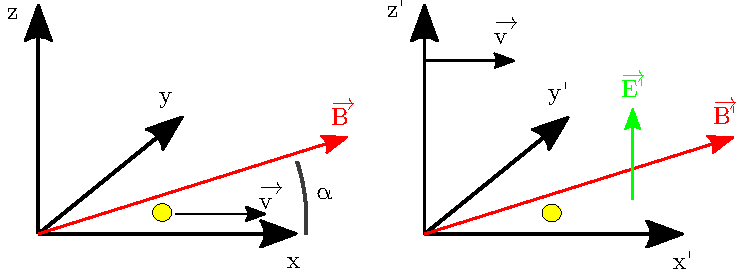
\includegraphics[width=0.7\textwidth]{04_Introduction/Images/non_thermal_emission/synchrotron_frames.pdf}
	\caption {An electron travelling at velocity $\vec{v}$ in the x-direction of the lab frame (\textit{left}) with a uniform magnetic field on the x-y plane at angle $\alpha$ to the x-axis. The rest frame of the particle (\textit{right}) travels at velocity $\vec{v}$ to the lab frame. The pure magnetic field $\vec{B}$ (i.e. no electric fields) in the lab frame appears as a mixture of magnetic field $\vec{B}'$ and electric field $\vec{E}'$ in rest frame.}
	\label{fig:chapter_1_non_thermal_sync_frames}
\end{figure}
\par~\par 
In the particles rest frame ($\vec{v}=0$), the force acted on the particle is described by:

\begin{equation}
	\begin{split}
		\vec{F}&=m\vec{a}=-e\qty(\vec{E}+\vec{v}\times \vec{B})  \\
		&=-e\vec{E}\text{ ,}
	\end{split}
\end{equation}
where $\vec{E}$ is the electric field strength in the particle's rest frame. For the example shown in \autoref{fig:chapter_1_non_thermal_sync_frames}, the parallel and perpendicular component of the electric field in the particle's rest frame can be obtained using Lorentz transformations:

\begin{subequations}
	\begin{align}
		\vec{E}_\parallel'&=\vec{E}_\parallel=0 \\
		\vec{E}_\perp'&=\gamma\qty(\vec{E}_\perp +\vec{v}\times \vec{B}_\perp) = E_z' = \gamma vB\sin\alpha\text{ .}
	\end{align}
\end{subequations}
\noindent Therefore the power radiated is given by:

\begin{equation}
    \begin{aligned}
	P&=-\frac{\qty(\gamma evB\sin\alpha/m)^2e^2}{6\pi\epsilon_0c^3}\text{ ,}
    \end{aligned} \label{eq:chapter_1_non_thermal_sync_power}
\end{equation}
\noindent where the negative in \autoref{eq:chapter_1_non_thermal_sync_power} represents the energy lost by the particle. Power is Lorentz invariant, hence \autoref{eq:chapter_1_non_thermal_sync_power} applies to both the lab and rest frame in \autoref{fig:chapter_1_non_thermal_sync_frames}. Electrons radiate more power via synchrotron radiation than protons of the same energy due to the inverse proportionality of the particle's mass (see \autoref{eq:chapter_1_non_thermal_sync_power}). Henceforth, only synchrotron radiation from electrons will be considered. The power radiated by a single electron through synchrotron radiation is:

\begin{equation}
    \begin{aligned}
    P&=-2\sigma_T\gamma^2c U_B\sin^2\alpha\text{ ,}
    \end{aligned}
\end{equation}
\noindent with the magnetic energy density defined to be $U_B=B^2/2\mu_0$ and the Thompson cross section is defined as:

\begin{equation}
    \begin{aligned}
    \sigma_T&=\frac{8\pi}{3}\qty(\frac{e^2}{4\pi\epsilon_0m_ec^2})^2=\frac{8\pi}{3}r_0^2\text{ ,}
    \end{aligned}
\end{equation}
\noindent where $r_0={e^2}/{4\pi\epsilon_0m_ec^2}$ is the classical electron radius. For electrons travelling in random directions:

\begin{equation}
    \begin{aligned}
        \left\langle \sin^2\alpha \right\rangle&=\half \int_{-1}^1\sin^2\alpha\dd{\cos\alpha}=\frac{2}{3}\text{ .}
    \end{aligned}
\end{equation}
\noindent The mean power loss is given by:

\begin{equation}
    \begin{aligned}
    \left\langle P\right\rangle&=\dv{E}{t}=-\frac{4}{3}\sigma_T\gamma^2 c U_B\text{ .}
    \end{aligned} \label{eq:01_leptonic_sync_energy_loss}
\end{equation}

The spectrum, $P\qty(\nu)$, of synchrotron emission emitted by a single electron with pitch angle $\alpha$ and magnetic field $B$ is given by \citep{2007A&A...474..689M}:

\begin{equation}
    \begin{aligned}
    j \qty(\nu)&=\dv{N}{E}=\frac{\sqrt{3}e^3B\sin\alpha}{mc^2}\frac{\nu}{\nu_c}\int_{x=\nu/\nu_c}^{\infty}K_\frac{5}{3}\qty(t)\dd{t}\text{ ,}
    \end{aligned} \label{eq:01_nontherm_sync_indiv}
\end{equation}
\begin{SCfigure}[0.42][h!]
    \centering
    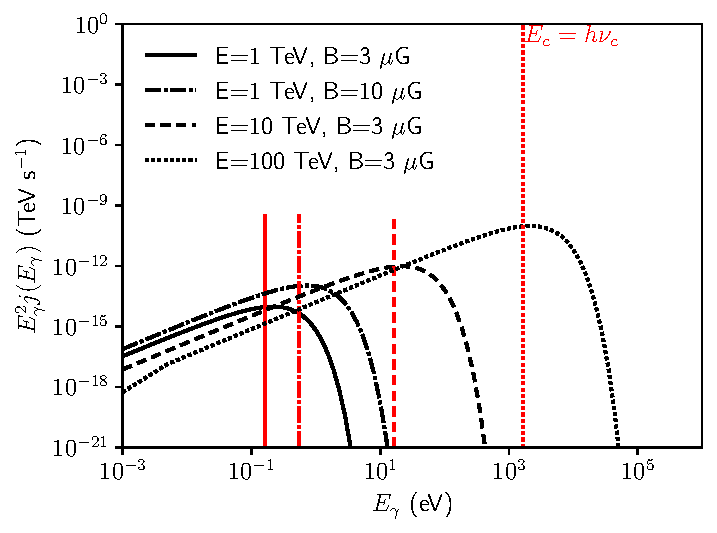
\includegraphics[width=0.7\textwidth]{04_Introduction/Images/non_thermal_emission/synchrotron_spectrum.pdf}
    \caption{Synchrotron emission from an electron with energy $E$ in magnetic field $B$. The red vertical lines represent the equivalent critical energy ($E_c=h\nu_c$).}
    \label{fig:01_sync_flux}
\end{SCfigure}
\noindent where $K_\frac{5}{3}$ is the modified Bessel function of the second kind. The synchrotron spectrum, $P\qty(\nu)$, peaks at `critical frequency' $\nu=\nu_c$ (see \autoref{fig:01_sync_flux}):
\begin{equation}
    \begin{aligned}
    \nu_c&=\gamma^2\frac{3eB\sin\alpha}{4\pi mc}\text{ .}
    \end{aligned}
\end{equation}
\noindent Equivalently, the synchrotron spectrum peaks at photon energy $E_\gamma$ \citep{2009ARA&A..47..523H}:

\begin{equation}
    \begin{aligned}
    \frac{E_\gamma}{\eV}&=0.087 \qty(\frac{E_e}{\TeV})^2 \frac{B}{\si{\micro G}}\text{ ,}
    \end{aligned}
\end{equation}
\noindent where $E_e$ is the energy of the initial electron. Therefore, observations of synchrotron emission $\gtrsim 300~\keV$ is a strong indicator of a source accelerating electrons up to $\PeV$ energies.

\subsubsection{Inverse-Compton emission}

Inverse-Compton emission occurs when an electron scatters off a photon:

\begin{align}
	\gamma_\text{low E} + e^{-'}&\rightarrow \gamma_{\TeV}+e^{-}\text{ ,}
\end{align}
where the final photon energy is greater than the original photon energy at cost of the electron energy ($E_{e^{-'}}>E_{e^-}$). Photon fields such as the CMB, infra-red photons, visible light, UV and X-rays provide target photons for the electron to scatter up to $\gamma$-ray energies. 
\par~\par
\begin{figure}[h!]
	\centering
	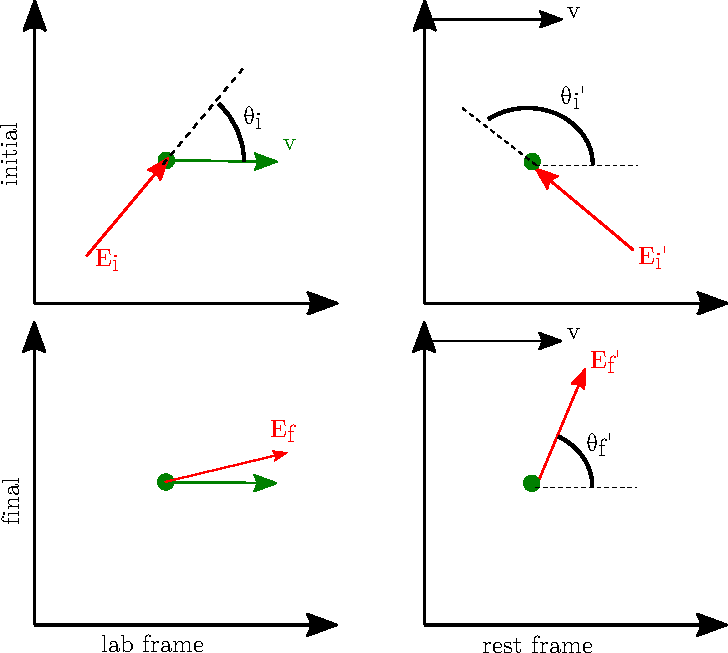
\includegraphics[width=0.7\textwidth]{04_Introduction/Images/non_thermal_emission/inverse_compton.pdf}
	\caption{A photon with energy $E_i$ scatters of an electron (travelling at velocity $v$) at angle $\theta$ in the lab frame (\textit{left}). In the rest frame of the electron (\textit{right}), the photon collides with electron at angle $\theta'$ and energy $E_i'$. The top and bottom panels describe the situation before and after the collision respectively. After scattering the photon has energy $E_f$ and $E_f'$ in the lab frame and electron rest frame respectively}
	\label{fig:chapter_1_non_thermal_compton_rest_frames}
\end{figure}
\autoref{fig:chapter_1_non_thermal_compton_rest_frames} shows a photon with momentum $\qty[\frac{E_i}{c},\frac{E_i}{c}\cos\theta_i,\frac{E_i}{c}\sin\theta_i,0]$ scattering off an electron in the lab and rest frame of the electron. The Lorentz transformation of the initial photon energy from the lab frame ($E_i$) to the rest frame ($E_i'$) is given by:

\begin{equation}
    \begin{aligned}
        E_i'&=\gamma E_i\qty(1-\beta \cos\theta_i)\text{ ,}
    \end{aligned}    
\end{equation}
\noindent where $\beta = v/c$ and $v$ is the electron velocity. The Lorentz transformation of the final photon energy from the rest frame to the lab frame is given by:

\begin{equation}
	\begin{aligned}
		E_f&=\gamma E_f'\qty(1+\beta\cos\theta_f')\text{ .}
    \end{aligned}
\end{equation}
\noindent Assuming elastic scattering, the photon has the same energy before and after the collision in the rest frame of the of the electron ($E_i'=E_f'$). Therefore the final energy in the lab frame is:

\begin{equation}
    \begin{aligned}
		E_f&=\gamma^2E_i\qty(1-\beta\cos\theta_i)\qty(1+\beta\cos\theta_f')\text{ .}
	\end{aligned}
\end{equation}
\noindent The photon scatters of the electron isotropically ($i.e.\left\langle\cos\theta_f'\right\rangle\approx 0$):

\begin{equation}
    \begin{aligned}
    \left\langle E_f\right\rangle&=\qty(1-\beta\cos\theta_i)\gamma^2 E_i\text{ .}
    \end{aligned}
\end{equation}
\noindent The rate of interaction, $R$, for electrons in photon field with density $n$ at angle $\theta_i$ can be described by:

\begin{equation}
    \begin{aligned}
    R&=n\sigma_T\qty(1-\beta\cos\theta_i)\text{ ,}
    \end{aligned}
\end{equation}
\noindent where $\sigma_T$ is the Thompson cross section. The rate of electron energy loss over a solid angle $\dd{\Omega}=2\pi\sin\theta_i\dd{\theta}=2\pi~\dd{\qty(\cos\theta_i)}$ is given by:

\begin{equation}
	\begin{split}
		\dv{E}{t}&=-\frac{\dd{\Omega}}{4\pi}Rc\left\langle E_f\right\rangle \\
		&=-nE_i\sigma_T c\gamma^2\frac{\dd{\cos\theta}}{2}\qty(1-\cos\theta_i)^2\text{ .}
	\end{split}
\end{equation}
\noindent Integrating over all $\theta_i$ gives the electron energy loss for Inverse Compton Interactions as:

\begin{equation}
    \begin{aligned}
    \dv{E_e}{t}&=-\frac{4}{3}U_\text{rad}\sigma_T c\gamma^2 \text{ ,}
    \end{aligned}   \label{eq:chapter_1_non_thermal_IC_e_energy_lost}
\end{equation}
\noindent where $U_\text{rad}=n\qty(E_i)E_i$ is the radiation energy density and $n\qty(E_i)$ is the number density.
\par~\par
The number density of target photons provided by photon fields such as the CMB can be described by a blackbody spectrum (see \autoref{sec:06_blackbodies}). Therefore, the spectrum from a single electron with energy $E_e$ scattering of a target photon with energy in range $\epsilon + \dd{\epsilon}$ is described by \citep{RevModPhys.42.237}:

\begin{equation}
    \begin{aligned}
        \frac{\dd{N}}{\dd{E_\gamma}}&=\frac{3\sigma_T mc^3}{4\gamma}\int_{E_\gamma/4\gamma^2}^{E_\gamma}\frac{n\qty(\epsilon)\dd{\epsilon}}{\epsilon}f\qty(q,\Gamma) \\
        f\qty(q,\Gamma)&=2q\ln q +\qty(1+2q)\qty(1-q)+\half\frac{\qty(\Gamma q)^2}{1+\Gamma q}\qty(1-q)\text{ ,}
    \end{aligned} \label{eq:01_nonthermal_IC_indiv_spectral}
\end{equation}
\noindent where:

\begin{subequations}
    \begin{align}
        q&=\frac{E_\gamma}{\Gamma\qty(E_e-E_\gamma)} \\
        \Gamma&=\frac{4\epsilon\gamma}{m_ec^2}\text{ .}
    \end{align}
\end{subequations}
\noindent $\Gamma$ determines whether the scattering falls under the Thompson limit ($\Gamma \ll 1$) or Klein-Nishina limit ($\Gamma \gtrsim 1$). The Thompson limit applies when the product of the incident and scattered photon energy is much less than the square of hte rest mass of the electron \citep{RevModPhys.42.237}. The Klein-Nishina limit  takes in account the suppression of IC scattering for relativistic electrons.
\begin{SCfigure}[0.42][h!]
    \centering
    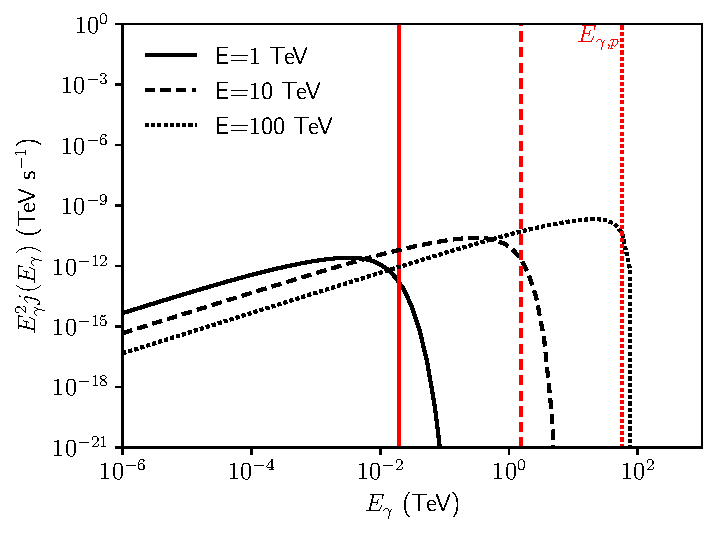
\includegraphics[width=0.7\textwidth]{04_Introduction/Images/non_thermal_emission/IC_spectrum.pdf}
    \caption{IC spectrum from an electron of energy $E$ interacting with the CMB.  The red vertical lines represent the energy at which the IC emission approximately peaks assuming a CMB photon has energy $\approx 7\times 10^{-4}~\eV$.}
    \label{fig:01_IC_flux}
\end{SCfigure}
\par~\par
In the Thompson regime, the inverse-Compton emission peaks at \citep{2009ARA&A..47..523H}:

\begin{equation}
	\begin{split}
		\frac{E_{\gamma,p}}{\TeV}&\approx \frac{E_e}{\TeV}\frac{2.1b}{\qty(1+\qty(2.1b)^{0.8})^{1/0.8}} \\
		b&\approx 15\frac{E_e}{\TeV}\frac{\epsilon}{\eV}\text{ .}
	\end{split} \label{eq:01_non_thermal_IC_max}
\end{equation}
\noindent \autoref{eq:01_non_thermal_IC_max} is used to approximate the energy range of the cosmic ray electron population. In the Klein-Nishina regime, \cite{doi:10.1126/science.abg5137} makes the approximation:

\begin{equation}
    \begin{aligned}
    \frac{E_e}{\PeV}&=2.15 \qty(\frac{E_{\gamma,p}}{\PeV})^{0.77}\text{ ,}
    \end{aligned}
\end{equation}
which is accurate to within $10\%$ for electrons within energy range $[30~\TeV,3~\PeV]$. Therefore, observations of gamma rays with energy $\gtrsim 200~\TeV$ from IC interactions is a strong indicator that the source is a leptonic PeVatron (see \autoref{sec:chapter_1_PeVatrons}).

\subsubsection{Bremsstrahlung Emission}

Bremsstrahlung emission occurs when an electron experiences deacceleration due to the presence of an atomic nucleus. For a single electron with energy $E_e$ passing through a gas with number density $n$, the radiated photon spectrum per electron can be described by \citep{RevModPhys.42.237}:

\begin{equation}
	\begin{split}
		\frac{\dd{N}}{\dd{t}\dd{k}}&=cn\dd{\sigma} \text{ ,}
	\end{split} \label{eq:chapter_1_non_thermal_brem_SED}
\end{equation}
\noindent where the electron has initial \& final energy, $E_i$ \& $E_f$ respectively. By conservation of energy, the final photon has energy $k=E_i-E_f$. The differential cross section, $\dd{\sigma}$, can be written as \citep{1934RSPSA.146...83B}:

\begin{equation}
	\begin{split}
		\dd{\sigma}&=\alpha r_0^2\qty(\frac{\dd{k}}{k})\frac{1}{E_i^2}\qty[(E_i^2+E_f^2)\phi_1-\frac{2}{3}E_i E_f\phi_2]\text{ ,} \label{eq:chapter_1_non_thermal_brem_cross_section} 
	\end{split}
\end{equation}
\noindent with $\alpha=1/137$ is the fine structure constant and for a unshielded charge:
\begin{equation}
    \begin{aligned}
        \phi_1&\approx\phi_2=4Z^2\qty[\ln(\frac{2E_iE_f}{k})-\half]\text{ .}
    \end{aligned}
\end{equation}
\par~\par
The SED of Bremsstrahlung emission is proportional to the density of the ambient medium (see \autoref{eq:chapter_1_non_thermal_brem_SED}). Therefore in cases such as pulsar wind nebuae, where the ISM has been "swept" out by the progenitor stellar wind, inverse Compton and synchrotron emission will generally dominate over Bremsstrahlung emission. The electron energy loss rate, as derived by \cite{RevModPhys.42.237}, for an electron interacting with ambient gas with density $n_z$ and atomic number $Z$ is related by:

\begin{equation}
    \begin{aligned}
    \dv{E_e}{t}&=-\frac{n_z Z\qty(Z+1.3)e^6}{16\pi^3\hbar \epsilon_0^3 m_ec^4}E_e\qty[\ln(\frac{183}{Z^{\third}})+\frac{1}{8}]\text{ .}
    \end{aligned} \label{eq:01_leptonic_brem_energy_loss}
\end{equation}

\subsubsection{Total Leptonic Radiative Processs}

The cooling time of an interaction, the time it takes for an electron to cool to a lower kinetic energy, can be used to determine the dominant process amongst the three leptonic processes (synchrotron, inverse Compton and Bremsstrahlung). The cooling time is defined to be:

\begin{equation}
    \begin{aligned}
        \tau&=\int_{\gamma'}^\gamma \frac{\dd{\gamma''}}{\dot{\gamma}} \\
        &\approx \frac{\gamma}{\dot{\gamma}}\text{ for }\gamma'\approx \gamma\text{ ,}
    \end{aligned}
\end{equation}
\noindent where an electron cools from Lorentz factor $\gamma'$ to $\gamma$ at rate $\dot{\gamma}\qty(\gamma'')$. The cooling time for synchrotron, inverse Compton and Bremsstrahlung interactions are given by \citep{2009ARA&A..47..523H}:

\begin{subequations}
    \begin{alignat}{1}
        \tau_\text{sync} &\approx 1.3\times 10^7 \qty(\frac{B}{\si{\micro G}})^{-2}\qty(\frac{E_e}{\TeV})^{-1}\quad\qty[\si{yr}] \label{eq:chapter_1_non_thermal_sync_cooling_time} \\
        \tau_\text{IC}&=3\times 10^5 \qty(\frac{U_\text{rad}}{\si{\electronvolt\per\centi\meter\cubed}})^{-1}\qty(\frac{E_e}{\TeV})^{-1}\mathscr{f}^{-1}\quad\qty[\si{yr}] \label{eq:chapter_1_non_thermal_IC_cooling_time} \\
        \tau_\text{brem}&\approx 3.9\times 10^7 \qty(n/\centimeterminusthree)^{-1}\quad\qty[\si{yr}]\text{ ,} \label{eq:chapter_1_non_thermal_brem_cooling_time}
\end{alignat} \label{eq:chapter_1_non_thermal_cooling_time}
\end{subequations}
\noindent where:

\begin{equation}
    \begin{aligned}
    \mathscr{f}\qty(\gamma,\epsilon_0)&=\qty(1+4\gamma\epsilon_0)^{-\frac{3}{2}}\text{ ,}
    \end{aligned}
\end{equation}
\begin{figure}[h!]
		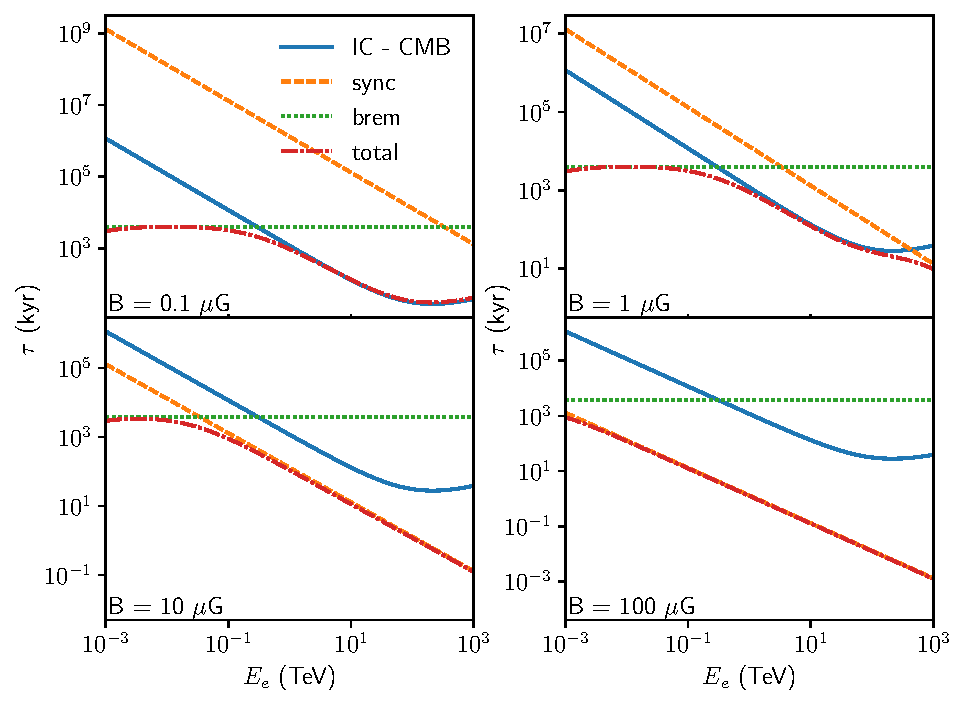
\includegraphics[width=0.99\textwidth]{04_Introduction/Images/non_thermal_emission/cooling_time_final.pdf}
		\caption{Cooling times for electrons at different energies in a uniform cloud with density $n=10~\centimeterminusthree$ and magnetic field $B = 0.1$, $1$, $10$ \& $100~\si{\micro G}$. The solid blue line shows the cooling time for inverse-Compton interactions against the CMB ($U_\text{CMB}=0.26\si{\electronvolt\per\centi\meter\cubed}$). The dashed yellow line shows the cooling time for synchrotron interactions while the dotted green line shows the cooling time for Bremsstrahlung interactions.}
		\label{fig:chapter_1_non_thermal_emission_lep_cooling_losses}
\end{figure}
\noindent considers the Thompson limit or Klein-Nishina limit of inverse-Compton scattering with a photon with dimensionless energy $\epsilon_0=h\nu/m_ec^2$ and frequency $\nu$. \cite{2007A&A...474..689M} describes the total cooling rate as:
\begin{equation}
    \begin{aligned}
    \dot{\gamma}_\text{total}&=b_s\gamma^2+\sum_{i} b_\text{IC}\gamma^2F_\text{KN}\qty(\gamma)+b_C\qty(\ln \gamma+b_C^0)+b_B\gamma\qty(\ln\gamma+b_B^0) \text{ ,}
    \end{aligned} \label{eq:chapter_1_non_thermal_leptonic_cooling_rate}
\end{equation}
where $\sum_{i}$ sums over all radiation fields contributing to the Inverse-Compton gamma-ray flux. The coefficients $b$:

\begin{itemize}[noitemsep]
	\item $b_s=\frac{4\sigma_T}{3m_ec}u_B=1.292\times 10^{-15}\qty(B/\si{\milli G})^2~\qty[\persec]$ which is a synchrotron loss constant.
	\item $b_\text{IC}=b_s\frac{u_0}{u_B}=5.204\times 10^{-20}\qty(u_0/\si{\electronvolt\per\centi\meter\cubed})~\qty[\persec]$ which is an inverse Compton constant.
	\item $b_C=\frac{2\pi e^4 n_e}{m_e^2 c^3}=1.491\times 10^{-14}n_e~\qty[\persec]$ which is the Coulomb loss constant.
	\item $b_B=\frac{4e^6 n_e}{m_e^2c^4\hbar}=1.37\times 10^{-16}n_e~\qty[\persec]$ which is the Bremsstrahlung loss constant.
	\item $b_C^0=\ln(\frac{m_e^3c^4}{4e^2n_e\hbar^2})+\frac{3}{4}=-\ln n_e+73.4$
	\item $b_B^0=\ln 2-\third=0.36$
\end{itemize}
\noindent and $m_e$ and $e$ being the mass \& charge of the electron respectively, $u_0$ and $u_B$ are the energy densities of the photon and magnetic fields and $n_e$ is the electron density number. The function $F_\text{KN}$ takes account the full Klein-Nishina cross section for Inverse Compton scattering \citep{2007A&A...474..689M}:

\begin{equation}
	\begin{split}
		F_\text{KN}&=\frac{1}{u_0}\int_{0}^\infty \mathscr{f}\qty(\gamma,\epsilon_0)u_{\epsilon_0}\dd{\epsilon_0} \text{ .}
	\end{split}
\end{equation}
\noindent For a Planckian black body distribution of photon energies, $F_\text{KN}$ can be approximated by:

\begin{equation}
    \begin{aligned}
    F_\text{KN}&=\qty(1+4\gamma \epsilon_\text{eff})^{-3/2} \\
    \epsilon_\text{eff}&=\frac{2.8kT}{m_ec^2}\text{ .}
    \end{aligned}
\end{equation}
\noindent For Bremsstrahlung losses in neutral hydrogen, \autoref{eq:chapter_1_non_thermal_leptonic_cooling_rate} becomes:

\begin{equation}
    \begin{aligned}
    \dot{\gamma}_\text{total}&=b_s\gamma^2+\sum_{i} b_\text{IC}\gamma^2F_\text{KN}\qty(\gamma)+b_C\qty(3\ln \gamma+18.8)+5.3b_B \text{ .}
    \end{aligned} \label{eq:chapter_1_non_thermal_leptonic_cooling_rate2}
\end{equation}
\noindent \autoref{fig:chapter_1_non_thermal_emission_lep_cooling_losses} shows the individual and total cooling time for electrons for different electron energies in a uniform cloud with varying magnetic field strengths. Synchrotron losses dominate in high magnetic fields and/or high electron energies. For example, synchrotron losses are dominant for electrons greater $\approx 85~\TeV$ than in a magnetic field of $3~\si{\micro G}$ and dominant for magnetic fields greater than $\approx 12~\si{\micro G}$ for $1~\TeV$ electrons scattering against CMB photons ($u_0=0.26~\si{\electronvolt\per\centi\meter\cubed}$ and $T=2.7~\si{\kelvin}$). 
\par~\par 
\autoref{fig:01_sync_flux} and \autoref{fig:01_IC_flux} shows the synchrotron and IC emission from a single electron energy. The SED from an electron distribution $J_e\qty(E_e)$ is described by:

\begin{equation}
    \begin{aligned}
        \Phi\qty(E_\gamma)= \int_{E_\gamma}^\infty J_e\qty(E_e) F_\gamma(E_\gamma,E_e)\dd{E_e}\text{ ,}
    \end{aligned} \label{eq:01_non_thermal_leptonic_total}
\end{equation}
\noindent where $F_\gamma(E_\gamma,E_e)\dd{E_e}$ is given by \autoref{eq:01_nontherm_sync_indiv}, \autoref{eq:01_nonthermal_IC_indiv_spectral} and \autoref{eq:chapter_1_non_thermal_brem_SED}. Overall, the flux ratio of IC to and synchrotron emission in the Thompson regime is related by \citep{1997MNRAS.291..162A}:

\begin{equation}
    \begin{aligned}
    \frac{f_\text{IC}\qty(E)}{f_s\qty(E)}&=\frac{U_\text{rad}}{U_B}\text{ .}
    \end{aligned} \label{eq:chapter_IC_2_sync_ratio}
\end{equation}
\par~\par
Electrons escaping the PWN cool at a rate that is dependent on the surrounding environment (\autoref{eq:chapter_1_non_thermal_leptonic_cooling_rate2}), affecting the energy distribution of cosmic rays and the subsequent multiwavelength emission (\autoref{eq:01_non_thermal_leptonic_total}). Therefore, \autoref{sec:07_particle_ev} will describe the evolution of cosmic rays (leptonic and hadronic) and the subsequent SED.

\chapter{Gamma Ray Astronomy} \label{sec:02_astronomy}

\autoref{sec:01_PWN_chapter} discussed how PWNe like \mbox{HESS\,J1825-137} accelerate cosmic rays up to $\TeV$ energies and how gamma rays can be used as alternative messengers. To study accelerators like \mbox{HESS\,J1825-137}, astronomers require instruments that are capable of observing gamma rays up to $\TeV$ energies.
\par~\par 
Upon reaching the Earth atmosphere, gamma rays produce air showers comprising of billions of secondary particles and photons. Astronomers in the early 20th century placed Geiger counters on balloons to detect gamma rays at high altitude \citep{hess1912observations}. Now, satellites like \textit{Fermi}-LAT are used to observe gamma rays less than $\approx 0.1~\TeV$ before they enter the atmosphere \citep{2010RPPh...73g4901M}. Alternatively, ground-based observatories analyse the air shower itself to reconstruct information about the original gamma ray. This is a method used by the High Energy Stereoscopic System (H.E.S.S.) to study $\TeV$ gamma-ray sources like \mbox{HESS\,J1825-137}.
\par~\par 
This section will provide a brief overview of how gamma rays interact with the atmosphere and the techniques used to observe the subsequent shower of particles. Finally, there will be a description of the gamma-ray observatories whose data products were utilised in this thesis.% in particular the High Energy Stereoscopic System (H.E.S.S.).

\section{Air Showers}

The presence of molecules in the atmosphere provides a target for gamma rays and cosmic-ray protons to interact and produce lower energy particles (electrons, positrons, pions). The daughter particles then go on to decay or interact with the atmosphere to produce even lower energy particles. This process cascades to form an air shower which is shown in \autoref{fig:chapter_2_air_shower_em} and \autoref{fig:chapter_2_air_shower_hadron}.
\par~\par 
The morphology and structure of the air shower is dependent on the atmosphere. Atmospheric depth is defined to be the attitudinal integral of atmospheric density above height $h$ \citep{alma9924446790001811}:

\begin{equation}
    \begin{aligned}
    X&=\int_{h}^\infty \rho\qty(h')\dd{h'}\text{ ,}
    \end{aligned}
\end{equation}
\noindent with the units of atmospheric depth being $\grampercentimetresquared$. Atmospheric depth is a proxy for the amount of material above height $h$. For a constant temperature, the relationship between height and atmospheric depth becomes:

\begin{equation}
    \begin{aligned}
    X=X_0\exp(-h/h_0)\text{ ,}
    \end{aligned}
\end{equation}
where $h_0$ is the scale height of the atmosphere and $X_0=1030~\grampercentimetresquared$ is the atmospheric depth at sea level. 
\subsection{Gamma-ray Air Showers} \label{sec:05_air_shower_gamma_ray}
To produce an electron-positron pair, a gamma ray must be in the vicinity of a nucleus to conserve both momentum and energy. When a gamma ray above a few $\GeV$ enters the atmosphere, the presence of atmospheric nuclei allows pair production to occur:
\begin{equation}
    \begin{aligned}
    \gamma + Z &\rightarrow e^- + e^+
    \end{aligned}
\end{equation}
\noindent where the daughter electron and positron each have kinetic energy:
\begin{equation}
    \begin{aligned}
    E_{e^\pm}&\approx \half\qty(E_\gamma-2m_ec^2)\text{ ,}
    \end{aligned} \label{eq:05_gamma_astrom_pair_condition}
\end{equation}
\noindent with $E_\gamma$ being the energy of the original gamma ray. Hence, the original gamma ray must have a threshold energy of twice the rest mas of the electron ($m_ec^2=511~\keV$) to undergo pair production.
\par~\par
Electrons and positrons interact with atmospheric nucleii through Bremsstrahlung interactions (see \autoref{sec:chapter_1_leptonic_gre}), resulting in the production of photons:

\begin{equation}
    \begin{aligned}
    e_\pm' + Z & \rightarrow e_{\pm} + Z + \gamma
    \end{aligned}
\end{equation}
\noindent with a cross section, $\dd{\sigma}_\text{brem}$, described by \autoref{eq:chapter_1_non_thermal_brem_cross_section} . The distance that an electron/positron travels before radiating a photon through Bremsstrahlung interactions is given by \citep{MATTHEWS2005387}:

\begin{equation}
    \begin{aligned}
    d=\lambda_r \ln 2\text{ ,}
    \end{aligned}
\end{equation}
\noindent where the radiation length, $\lambda_r$, is characteristic to a material and relates to the energy loss of high-energy particles as it transverses through a medium.
\par~\par 
Positrons can also annihilate with atmospheric electrons to produce two photons:

\begin{equation}
    \begin{aligned}
    e^- + e^+&\rightarrow \gamma + \gamma
    \end{aligned}
\end{equation}
with each daughter photon having threshold energy $E_\text{thr}\geq m_ec^2$. If the daughter photons have energy greater than twice the rest mass of an electron (\autoref{eq:05_gamma_astrom_pair_condition}), they can undergo electron-positron production. The cross section for electron-positron production, $\sigma_\text{pair}$, can be given in terms of the cross section for Bremsstrahlung interactions, $\sigma_\text{br}$, by:

\begin{equation}
    \begin{aligned}
    \sigma_\text{pair}\qty(E_e,_E\gamma)&=\sigma_\text{br}\qty(E_e,E_\gamma)\frac{E_e^2}{E_\gamma^2}\approx \frac{7}{9}\sigma_\text{br}\qty(E_e,E_\gamma)\text{ ,}
    \end{aligned} \label{eq:chapter_2_pair_prod_cs}
\end{equation}
where $k$ is the energy of the resulting photons.
\begin{SCfigure}[1][h!]
    % \centering
    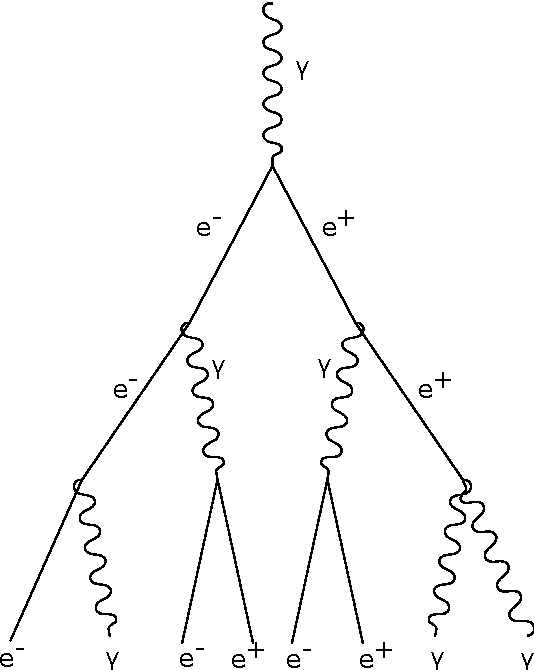
\includegraphics[width=0.5\textwidth]{05_Astronomy/Images/air_shower/gamma_ray.pdf}
    \caption{Heitler's model of the formation of an air shower triggered by a gamma ray \citep{1954qtr..book.....H}. The gamma ray undergoes pair production to produce an electron and positron. In turn, the electron/positron undergo Bremsstrahlung interactions and/or electron-positron annihilation to produce photons. This process cascades into the air shower.}
    \label{fig:chapter_2_air_shower_em}
\end{SCfigure}2
\par~\par 
Heitler's model of electromagnetic air showers (see \autoref{fig:chapter_2_air_shower_em}) provides a method to model the development of the electromagnetic shower \citep{1934RSPSA.146...83B}. It assumes that the radiation length for both pair production and Bremsstrahlung interactions are identical due to a similar cross section. Therefore, the atmospheric depth of the air shower after $n$ interactions is:

\begin{equation}
    \begin{aligned}
    X=nd=n\lambda_r\ln 2\text{ .}
    \end{aligned} \label{eq:chapter_2_gas_depth}
\end{equation}
\noindent The number of particles (electrons, positrons and photons) in the air shower after $n$ interactions is given by \citep{MATTHEWS2005387}:
\begin{equation}
    \begin{aligned}
    N&=2^n=\exp(X/\lambda_r)\text{ ,}
    \end{aligned}
\end{equation}
\noindent with the average particle energy after $n$ interactions being:

\begin{equation}
    \begin{aligned}
    E_n&=\frac{E_0}{2^n}=E_0\exp(-X/\lambda_r)\text{ ,}
    \end{aligned}
\end{equation}
\noindent where $E_0$ is the energy of the original gamma-ray photon that triggered the air shower.
\par~\par 
The exponential growth of the air shower continues until the daughter particles reach a critical energy $E_c$ ($\approx 85~\MeV$ in air) where ionisation losses dominate over radiative losses \citep{1954qtr..book.....H}. At this point, the shower has the maximum number of particles:

\begin{equation}
    \begin{aligned}
    N_\text{max}&=2^{n_c} = \frac{E_0}{E_c}\text{ ,}
    \end{aligned} \label{eq:chapter_1_gas_max_particles} 
\end{equation}
\noindent where $n_c$ is the number of interactions when critical energy is reached. Therefore:

\begin{equation}
    \begin{aligned}
    n_c&=\log_2 \frac{E_0}{E_c} =\frac{\ln{\frac{E_0}{E_c}}}{\ln 2}\text{ .}
    \end{aligned} \label{eq:chapter_2_gas_max_interactions}
\end{equation}
\noindent Therefore, the air shower depth after $n_c$ interactions:

\begin{equation}
    \begin{aligned}
    X_\text{max}&=\lambda_r \ln\frac{E_0}{E_c}\text{ .}
    \end{aligned} \label{eq:chapter_2_gas_max_depth}
\end{equation}
\noindent The elongation rate of an air shower is defined to be the rate of change of the depth of shower maximum with energy \citep{MATTHEWS2005387}:

\begin{equation}
    \begin{aligned}
    \Lambda=\dv{X_\text{max}}{\log_{10}E_0} \text{ .}
    \end{aligned} \label{eq:chapter_2_gas_elongation_length}
\end{equation}
\noindent Combining \autoref{eq:chapter_2_gas_max_depth} \& \ref{eq:chapter_2_gas_elongation_length} gives:

\begin{equation}
    \begin{aligned}
    \Lambda_\gamma &= 2.3\lambda_r ~ \text{per decade of primary energy}\text{ .}
    \end{aligned}
\end{equation}
\noindent In air, electromagnetic air showers have elongation rate of $85\grampercentimetresquared$ per decade of primary energy.
\par~\par

Further studies \citep{MATTHEWS2005387} showed that the the maximum number of electrons predicted by Heitler's model, $N_\text{e, H}$ overestimates the number of particles compared to that measured by experiments. \cite{MATTHEWS2005387} revised the maximum number of particles, $N_\text{e, M}$, to be:

\begin{equation}
    \begin{aligned}
    N_\text{e, M} &= \frac{N_\text{e, H}}{10} \text{ .}
    \end{aligned} \label{eq:chapter_2_gas_e_correction_factor}
\end{equation}
\noindent In summary, Heitler noted that in electromagnetic cascade showers \citep{1954qtr..book.....H}:

\begin{enumerate}
    \itemsep0em
	\item The maximum number of particles in the cascade is proportional to the energy of the initial gamma ray $E_{\gamma,0}$.
	\item The depth of the shower is proportional to $\log E_0$.
	\item The shower development is independent of the atmospheric `material' provided that atmospheric thickness is measured in cascade units and energy in units of critical energy.
    \item The angular spread of an electromagnetic shower is not large as the emission of light from Bremsstrahlung interactions and pair production is at small angles assuming the initiating particle has high energy.
\end{enumerate}
\noindent Overall, Heitlers model can be used to predict the basic electromagnetic air shower structure.

\subsection{Cosmic-ray Air Showers}
\begin{SCfigure}[1][h!]
    % \centering
    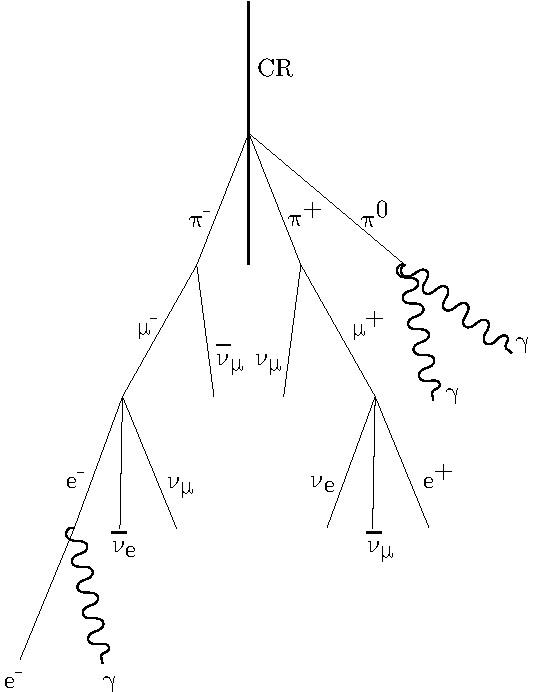
\includegraphics[width=0.5\textwidth]{05_Astronomy/Images/air_shower/cosmic_ray.pdf}
    \caption{The formation of an air shower triggered by a cosmic ray entering the atmosphere. The cosmic ray undergoes proton-proton interactions to produce neutral and charged pions. Neutral pions decay into two photons (which can trigger an electromagnetic air shower) while charged pions decay into muons and neutrinos. The muons decay into electrons/positrons and neutrinos. Depending on its energy, the original cosmic ray can undergo further proton-proton collision.}
    \label{fig:chapter_2_air_shower_hadron}
\end{SCfigure}
Both gamma rays and cosmic rays initiate air showers upon entering the atmosphere. Therefore, any observatory dedicated to studying gamma rays must be able to distinguish between a gamma-ray air shower and cosmic-ray air shower.
\par~\par
Cosmic rays (protons or nucleii) above a few $\GeV$ undergo proton-proton collisions (see \autoref{sec:chapter1_hadronic_gr_emission}) with atmospheric nuclei and produce pions.

\begin{equation}
    \begin{aligned}
    \text{CR} + p_\text{atmos} &\rightarrow \text{CR} + \pionneutral + \pionminus + \pionplus
    \end{aligned}
\end{equation}

\noindent where the ratio of charged pions to neutral pions is approximately $2:1$. Charged pions decay into neutrinos and muons, with muons then decaying into electrons, positrons, neutrinos and anti-neutrinos. The presence of muons in an air shower can indicate whether the shower was triggered by a gamma ray or cosmic ray. Electrons and positrons interact with the atmosphere via Bremstrahlung and electron-positron annihilation to produce photons as discussed in \autoref{sec:05_air_shower_gamma_ray}. Unlike gamma-ray air showers, the original cosmic ray can go on to undergo further proton-proton collisions to increase the number of charged pions in the atmosphere. This development of cosmic-ray air showers is shown in \autoref{fig:chapter_2_air_shower_hadron}.
\par~\par
The decay length, $d$, is defined to be the distance a particle with Lorentz factor $\gamma$ will travel before it decays \citep{MATTHEWS2005387}:

\begin{equation}
    \begin{aligned}
    d=\beta \gamma c \tau \text{ ,}
    \end{aligned}
\end{equation}
\noindent where ($\tau$ is the mean lifetime of the particle). The mean life time of charged pions is approximately $2.6\times 10^{-8}~\si{\second}$, while neutral pions have a mean life of $8.4\times 10^{-17}~\secs$. This gives the decay length for neutral and charged pions to be $d_{\pi_0}=\gamma \times  2.51 \times 10^{-6}~\cm$ and $d_{\pi_\pm}= 780\gamma~\cm$ respectively. Compared to charged pions, neutral pions decay essentially where they were created.
%Unlike Heitler's model of gamma-ray air showers, the radiation length for the decay of neutral and charged pions cannot be assumed to be identical.
\begin{SCfigure}[][h!]
    \centering
    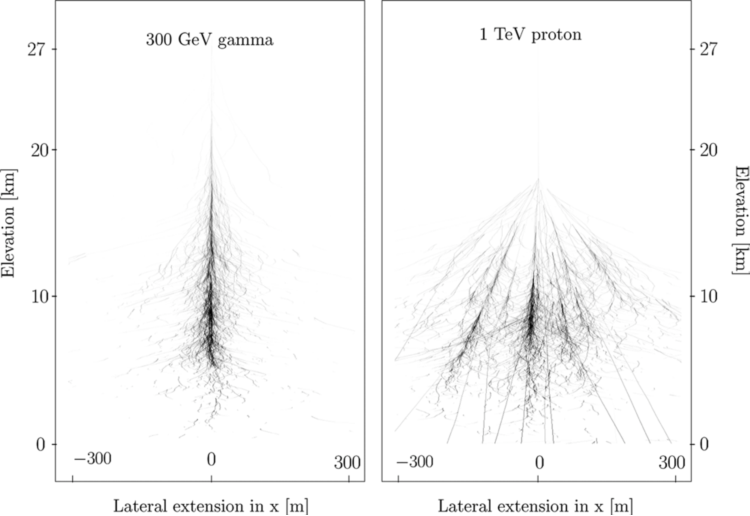
\includegraphics[width=0.7\textwidth]{05_Astronomy/Images/air_shower/cosmic_ray_vs_gamma_ray2.pdf}
    \caption{Monte Carlo simulations of a air shower triggered by a $0.3~\TeV$ gamma ray (\textit{left}) vs an air shower triggered by a $1~\TeV$ cosmic-ray proton (\textit{right}). Image courtesy of \cite{2008RPPh...71i6901A}}
    \label{fig:chapter_2_air_shower2}
\end{SCfigure}
\par~\par 
After $n$ interactions, there are $N_{\pi_\pm}$ charged pions with individual energy \citep{MATTHEWS2005387}:

\begin{equation}
    \begin{aligned}
    E_\pi &=\frac{E_0}{(\frac{3}{2}N_\text{ch})^n}\text{ ,}
    \end{aligned}
\end{equation}
\noindent where $E_0$ is the energy of the initial cosmic ray and $N_\text{ch}$ is the multiplicity of charged particles produced in hadronic interactions.
\par~\par
\cite{MATTHEWS2005387} gives the number of interactions (of the initial cosmic ray) for a pion to reach critical energy, $E_c^\pi$, to be:
\begin{equation}
    \begin{aligned}
    n_c&=\frac{\ln(E_0/E_c^\pi)}{\frac{3}{2}N_\text{ch}}=0.85\log_{10}\qty(\frac{E_0}{E_c^\pi}) \text{ ,}
    \end{aligned}
\end{equation}
\noindent occurring when the probability of pion decay exceeds the probability that it survives to the next interaction. The original energy of the cosmic ray is now divided between $N_\pi$ pions and $N_\text{max}$ electromagnetic particles:

\begin{equation}
    \begin{aligned}
    E_0&=N_\mu E_c^\pi + N_c^e N_\text{max} \\
 &\approx 0.85~\GeV\qty(N_e+24 N_\mu)\text{ ,}
    \end{aligned}
\end{equation}
\noindent where $N_e=N_\text{max}/10$ from \autoref{eq:chapter_2_gas_e_correction_factor}
\par~\par
The atmospheric depth where the number of air shower particles is at a maximum, $X_\text{max}^p$, is found through \citep{MATTHEWS2005387}:
\begin{equation}
    \begin{aligned}
    X_\text{max}^p&= X_0 + \lambda_r\ln(\frac{E_0}{3N_\text{ch}E_c^e}) =470+58\log_{10}\qty(E_0/1~\PeV)~\grampercentimetresquared \text{ ,}  
    \end{aligned}
\end{equation}
\noindent where $X_0$ is the atmospheric depth where the shower was initiated. The atmospheric depth maximum can be compared to the atmospheric depth maximum for gamma-ray air showers via:
\begin{equation}
    \begin{aligned}
    X_\text{max}^p=X_\text{max}^\gamma+X_0-\gamma_r\ln 3N_\text{ch}\text{ .}
    \end{aligned}
\end{equation}
\noindent This gives the elongation rate for proton initiated air showers:

\begin{equation}
    \begin{aligned}
    \Lambda^p &= \Lambda^\gamma + \dv{ }{\log_{10}E_0}\qty[X-\lambda_r\ln 3N_{ch}] \\
    &\approx 58~\grampercentimetresquared~\text{per decade of primary energy}\text{ .}
    \end{aligned}
\end{equation}
\noindent \autoref{fig:chapter_2_air_shower2} compares Monte Carlo simulations of air showers triggered by a $0.3~\TeV$ gamma ray and a $1~\TeV$ cosmic-ray proton, where the hadronic air shower is more spread out than gamma-ray air shower. Additionally, any photons produced by proton-proton interactions can trigger an electromagnetic shower within a hadronic air shower. Using this information, gamma-ray observatories can analyse the air shower to determine whether the initial particle was a gamma ray or proton.

\subsection{Cherenkov Light and Cherenkov Telescopes}

Particles produced in a electromagnetic air shower can travel faster than the speed of light in the atmosphere. The speed of light, $c_n$, in a medium with refractive index $n$ is given by:

\begin{equation}
    \begin{aligned}
    c_n = \frac{c}{n}\text{ ,}
    \end{aligned}
\end{equation}
\noindent where $c=3.0\times 10^8~\si{\meter\per\second}$ and $n>1$.
\par~\par 
A charged particle polarises the medium it is travelling through. As the particle propagates, the polarised medium oscillates back to its resting state and emits electromagnetic radiation. This is shown in \autoref{fig:chapter_2_chernkov_light}, where the resulting radiation can be described by Huygen's construction of light. For a particle that is travelling with velocity less than the speed of light, the electromagnetic radiation wave-fronts will destructively interfere with each other with no net production. If the charged particle is travelling faster than the speed of light in that medium, the electromagnetic wave-fronts will constructively interfere and there is a net production of light.
\par~\par
\begin{SCfigure}[1][h!]
    % \centering
    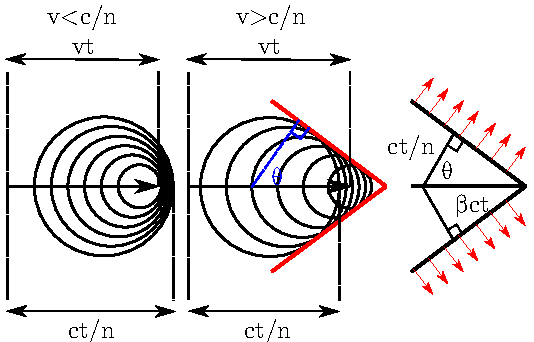
\includegraphics[width=0.5\textwidth]{05_Astronomy/Images/air_shower/chernkov_light.pdf}
    % \caption{ }
    \caption{Huygens's construction of a charged particle travelling at speed $v$ in a medium of refractive index $n$. Cherenkov light is emitted at angle $\theta$ when the particle is travelling faster than the speed of light in the medium}
    \label{fig:chapter_2_chernkov_light}
\end{SCfigure}
Cherenkov light is emitted in a cone in the direction of particle propagation (see \autoref{fig:chapter_2_chernkov_light}). At time $t=0$, a photon is emitted at angle $\theta$ to the particle propagation. After time $t$, the photon has travelled distance $ct/n$ and the particle has travelled $\beta ct$ ($\beta=v/c$, with v being the velocity of the particle). Hence:
\begin{equation}
    \begin{aligned}
    \cos\theta &= \frac{ct}{n} \frac{1}{\beta ct} \\
    &=\frac{1}{n\beta}\text{ .}
    \end{aligned}
\end{equation}
\noindent For ultra relativistic particles, $\beta\rightarrow 1$ and the light is emitted at angle $\theta \rightarrow \cos[-1](1/n)$.
\par~\par
The threshold for particle with mass $m$ to produce Cherenkov light occurs when it is travelling at the speed of light in a medium $(v=c/n)$:

\begin{equation}
    \begin{aligned}
    E_\text{thr}&=\gamma mc^2=\frac{mc^2}{\sqrt{1-{1}/{n^2}}}\text{ .}
    \end{aligned}
\end{equation}
\noindent For electrons at sea level ($n=1.0003$), the threshold energy is $\approx 21~\MeV$. In water, $n=1.33$, the threshold energy decreases to $1~\MeV$. Observatories such as the Pierre Auger observatory and the High Altitude Water Cherenkov gamma-ray observatory use water tanks (which has a higher refractive index $n=1.33$, hence slower speed of light than air) to produce Cherenkov light \citep{alma9924446790001811}.

\begin{figure}[h]
    \centering
    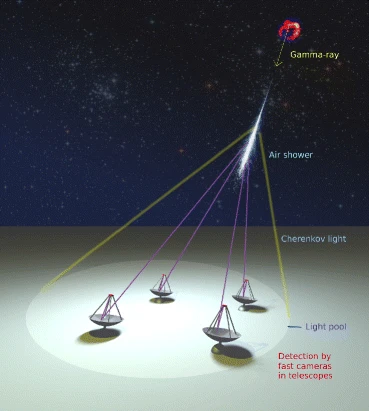
\includegraphics[height=0.4\textheight]{05_Astronomy/Images/air_shower/chenkov_light_pool.png}
    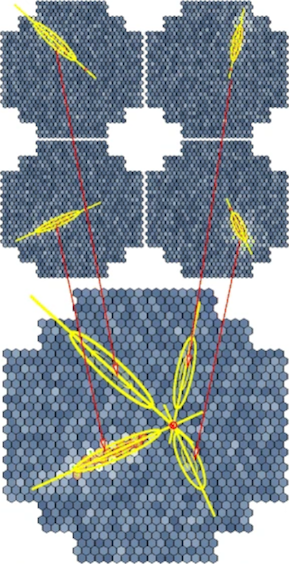
\includegraphics[height=0.4\textheight]{05_Astronomy/Images/air_shower/cherenkov_telescope.png}
    \caption{(\textit{left}) Pool of Cherenkov light from an air shower observed by four telescopes in a stereo system.
    (\textit{right}) Projection of the Cherenkov light onto one camera focal plane by the four telescopes. Images courtesy of \cite{2009ExA....25..173V,}.}
    \label{fig:chapter_2_chernkov_telescope}
\end{figure}
\par~\par
The air shower forms an observable pool of Cherenkov light on the ground as shown by the left-hand panel of \autoref{fig:chapter_2_chernkov_telescope}. At sea level, the radius of the light cone is approximately $125~\si{\meter}$ for a primary gamma ray of energy $0.1~\TeV$ but can extend to $1~\si{\kilo\meter}$ for energies greater than $100~\TeV$ \citep{Patterson_1983}.  A telescope can be placed anywhere within the light pool to detect the Chernkov light produced from particles in an air shower. Hence, the the effective collection area of the telescopes becomes the area of the light pool at the ground, which is of order $\approx1~\si{\kilo\meter\squared}$.
\par~\par
The top-right hand panel of \autoref{fig:chapter_2_chernkov_telescope} shows how Cherenkov light is observed by single and multiple telescopes. To characterise Cherenkov light, the light is first modelled by an ellipse and then parameters such as the width, length, location \& azimuthal angle to the center of the telescope is found. These parameters, known as the Hillas parameters \citep{1985ICRC....3..445H}, can be used to determine the arrival direction, energy and type of the particle that triggered the air shower. If multiple telescopes observe the same light at different angles, the combined image (see the right hand panel of \autoref{fig:chapter_2_chernkov_telescope}) can be reconstructed using `stereo' techniques with far more precision than if one telescope was used.

\section{TeV Gamma-ray Observatories} \label{sec:02_TeV_observatories}

Evidence of $\TeV$ gamma rays from AGN Centaurus were reported by \cite{1975ApJ...197L...9G}. But $\TeV$ astronomy effectively began with the detection of TeV gamma rays from the Crab Nebula \citep{1989ApJ...342..379W}. Over three decades later, $\TeV$ gamma rays from over 200 sources have been detected \citep{2008ICRC....3.1341W}. This section will describe some of the $\TeV$ gamma-ray observatories whose data pata products were used in this thesis.

\subsection{The High Energy Stereoscopic System} \label{sec:02_HESS}

\begin{figure}[h]
    \centering
    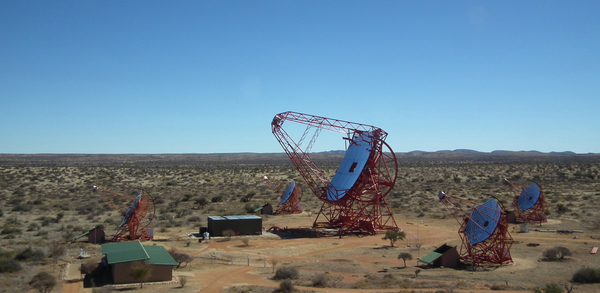
\includegraphics[width=\textwidth]{05_Astronomy/Images/telescopes/HESS_image.jpg}
    \caption{The High Energy Stereoscopic System. Images from \citep{HESS}.}
    \label{fig:chapter_2_HESS}
\end{figure}
\begin{figure}[h]
    \centering
    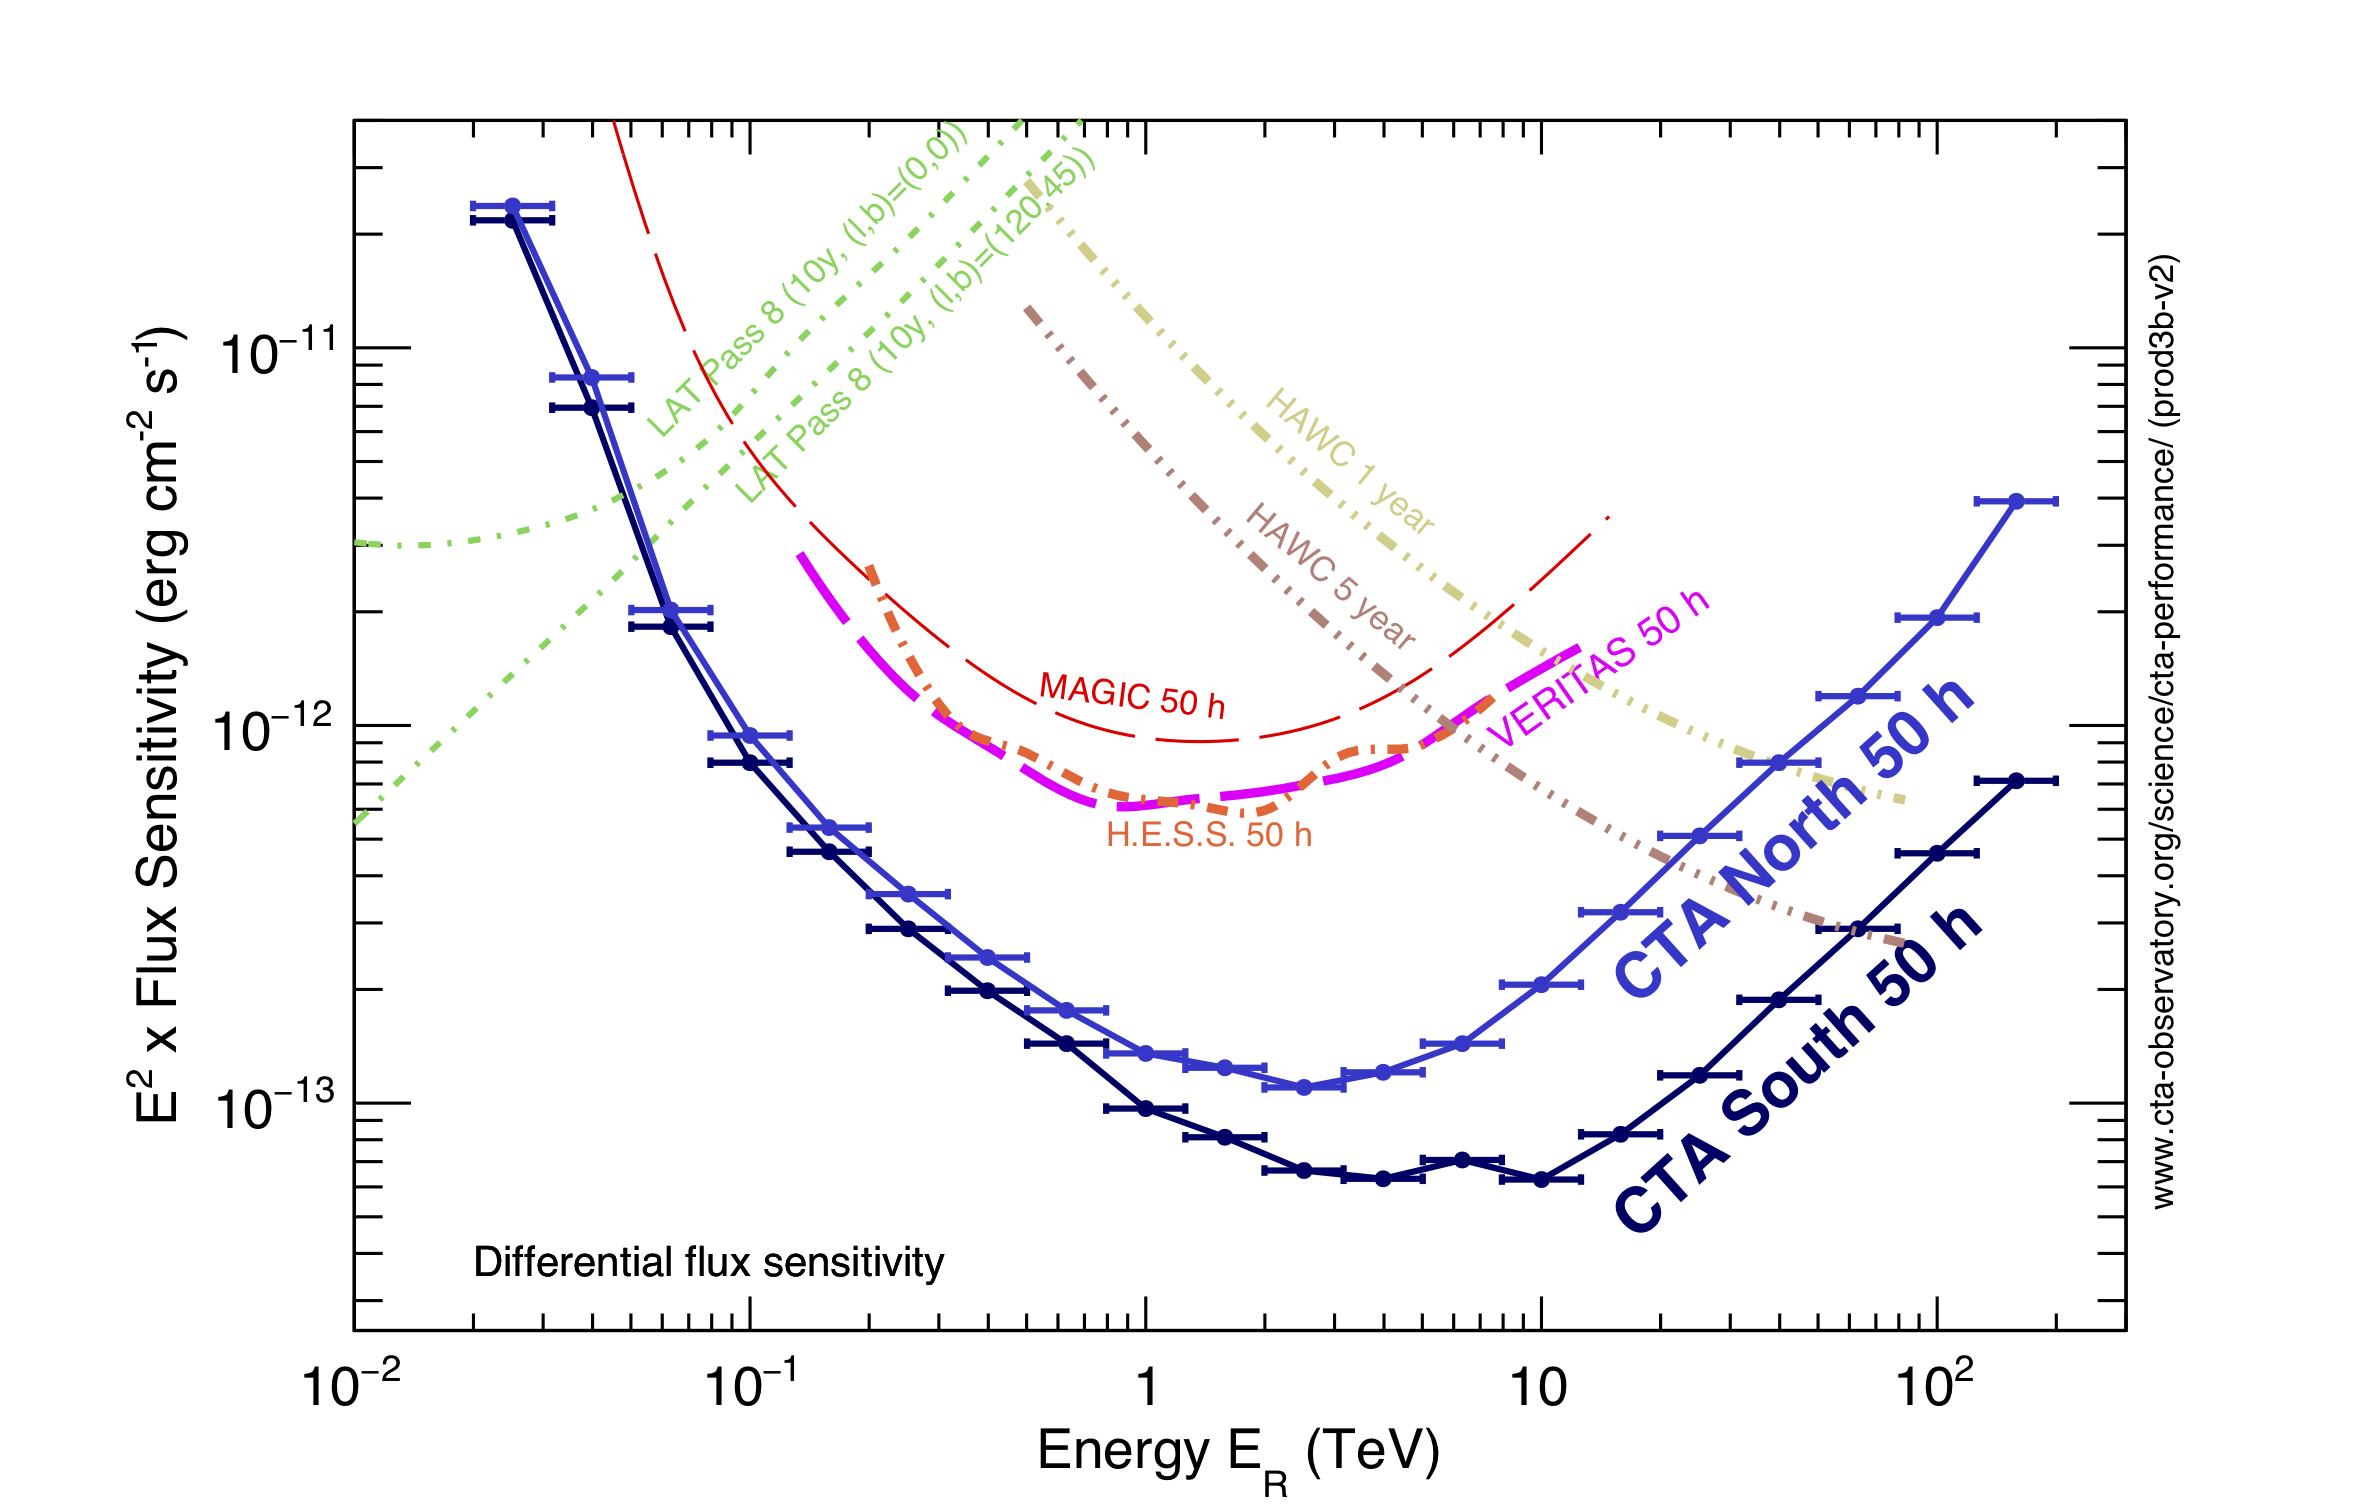
\includegraphics[width=0.9\textwidth]{05_Astronomy/Images/telescopes/sensitivity_comparison.png}
    \caption{Comparison of the performance (minimum detectable flux) of different gamma-ray instruments for an observation time of $50~\si{h}$. H.E.S.S., CTA south and CTA north is shown by the red, dark blue and light blue lines respectively. Image courtesy of \cite{2019scta.book.....C}.}
    \label{fig:chapter_2_sensitivity comparison}
\end{figure}

The High Energy Stereoscopic System (H.E.S.S.) telescope (named after Victor Hess) is an array of telescopes located at $1800~\si{\m}$ above sea lebvel in Namibia (see \autoref{fig:chapter_2_HESS}) \citep{HESS}. H.E.S.S. consists of five telescopes and utilises the atmospheric Cherenkov imaging technique described above to detect gamma radiation in the energy range $20~\GeV$ to $100~\TeV$. A comparison of the performance of H.E.S.S. to other instruments is shown in \autoref{fig:chapter_2_sensitivity comparison}. The angular resolution of H.E.S.S. ($\leq\ang{0.1}$) allows detailed observations of gamma-ray sources, which is key in understanding the morphology of objects such as SNRs and PWNe \citep{2018A&A...612A...1H}. HESS was constructed in two different phases; Phase I consisting of four $12~\m$ telescopes and Phase II added one $28~\m$ telescope at the centre of the array. Phase I and Phase II of H.E.S.S. commenced operations in December 2003 and July 2012 respectively. 
\par~\par 
The four $12~\m$ telescopes of Phase I have 382 mirror segments of $0.6~\m$ diameter mounted onto a steel frame in a Davies-Cotton optical layout (a parabolic layout where each mirror has focal length $f$, which is the focal length of the entire telescope ($15~\m$)) \citep{2003APh....20..111B}. The mirrors combine to have total mirror surface area of $107~\si{\meter\squared}$ and focus the Cherenkov light onto a photomultiplier camera (containing $\approx 1000$ pixels) with a $\ang{5}$ field of view. Each dish is mounted on a rotating base frame which rotates azimuthally on a rail of $13.6~\m$ diameter. The telescopes have a peak positioning speed of $100\si{^\circ\per\minute}$ in both azimuth and elevation and is sensitive to gamma rays above $100~\GeV$. This is ideal for observing events such as gamma-ray bursts and following up activity triggered by other observatories (e.g. neutrinos from IceCube, GRBs from Swift). The four telescopes are placed in a square geometry with distances $120~\m$ from each other.
\par~\par
Phase II of H.E.S.S. placed an additional $24~\m$ telescope in the centre of phase I \citep{2005ICRC....5..163V}. The telescope consists of 875 hexagonal mirrors of $0.9~\m$ sides laid out in a parabolic shape with focal length of $36~\m$ and total mirror area of $614~\si{\meter\squared}$. The Phase II telescope has azimuth and elevation speed of $200\si{^\circ\per\minute}$ and $100\si{^\circ\per\minute}$ respectively. Similar to Phase I, Phase II focuses Cherenkov light onto a photomultiplier camera consisting of $\approx 2000$ pixels with a $\ang{3.2}$ view of the sky.

\subsubsection{The H.E.S.S. Galactic Plane Survey}

\begin{figure}[h]
    \centering
    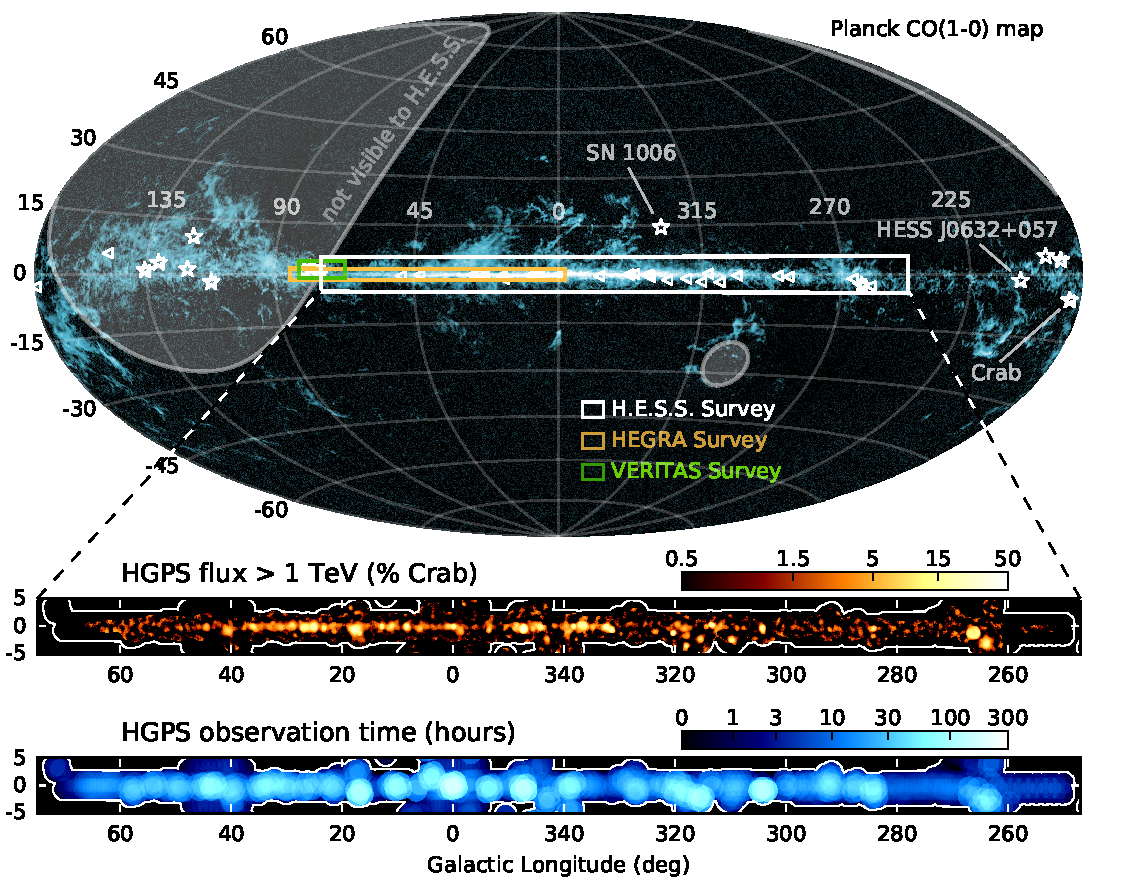
\includegraphics[width=0.9\textwidth]{05_Astronomy/Images/telescopes/hess_survey.pdf}
    \caption{The H.E.S.S. Galactic plane survey superimposed onto \textit{Planck} CO data. Image courtesy of \cite{2018A&A...612A...1H}.}
    \label{fig:chapter_2_HESS_survey}
\end{figure}

In 2018, H.E.S.S. released its third Galactic Plane Survey (HGPS) in $\TeV$ gamma rays that covers data from January 2004 to January 2013 totalling $2864\si{\hour}$ of observation time \citep{2018A&A...612A...1H}. The HGPS catalogued 78 very high energy (VHE) sources compared to 10 sources in the first release \citep{2005Sci...307.1938A} and  22 in its second \citep{2006ApJ...636..777A}. Of the 78 VHE sources; 3 are binary objects (composed of a massive star and a compact object), 8 are SNRs, 12 are PWN, 8 are composite objects (SNR + PWN), 11 have no known association and a further 36 are not firmly identified. \cite{2018A&A...612A...1H} found that 47 of the HGPS sources ($60\%$) had an associated pulsar and ($39\%$ being a PWN or a composite object (SNR + PWN). This makes PWNe the largest source class in the survey. Following the HPGS survey, \cite{2018A&A...612A...2H} conducted a study on the population of $\TeV$ PWN to link PWN evolutionary theory to $\TeV$ observations (see \autoref{sec:01_PWN_TeVPWN} for further detail). This thesis focuses on the $\TeV$ PWN \mbox{HESS\,J1825-137}.

\subsection{\textit{Fermi}-LAT}

The \textit{Fermi} Gamma-ray Space Telescope is a space based observatory launched on the 11th of June 2008. \textit{Fermi} has two instruments; the Large Area Telescope (LAT) and the Gamma-ray Burst Monitor \citep{2010RPPh...73g4901M}. \textit{Fermi}-LAT consists of thin metal sheets that assist in the production of electron-positron pairs. The electron-positron pair then pass through microstrip detectors that can track their trajectory. Finally, the products enter a calorimeter which measures the combined energy of the electron-positron pair to determine the energy of the initial gamma ray. The Gamma-ray Burst Monitor consists of scintillators positioned on opposite sides of the spacecraft allowing different viewing angles to detect gamma-ray bursts and solar flares \citep{2010RPPh...73g4901M}. The performance characteristic of \textit{Fermi}-LAT allows sensitivity in the energy range of $20~\MeV - 300~\GeV$ with a field of view of $2.4~\si{\steradian}$ \citep{2010RPPh...73g4901M}. 
\par~\par
The equivalent \textit{Fermi}-LAT source towards \mbox{HESS\,J1825-137} is \mbox{4FGL\,J1824.5\,1351e} \citep{2020ApJS..247...33A}. \cite{2020A&A...640A..76P} combined GeV data from \textit{Fermi}-LAT and $\TeV$ data from H.E.S.S. to provide a broader view of the gamma-ray emission towards \mbox{HESS\,J1825-137} from $1~\GeV$ up to $100~\TeV$. They found that the size of the PWN increases at lower energies, implying that electrons from the outer edges are from an older population of electrons compared to the recently injected electrons near the powering pulsar. This is indicative of a $\TeV$ halo forming, where electrons begin to escape the PWN into the ISM and emit $\TeV$ emission via inverse Compton interactions.

\subsection{LHAASO}

The Large High Altitude Air Shower Observatory (LHAASO) is a gamma-ray and cosmic-ray observatory located $\approx 4400~\m$ above sea level in Sichuan China \citep{2022ChPhC..46c0001M}. LHAASO consists of:
\begin{figure}[h!]
    \centering
    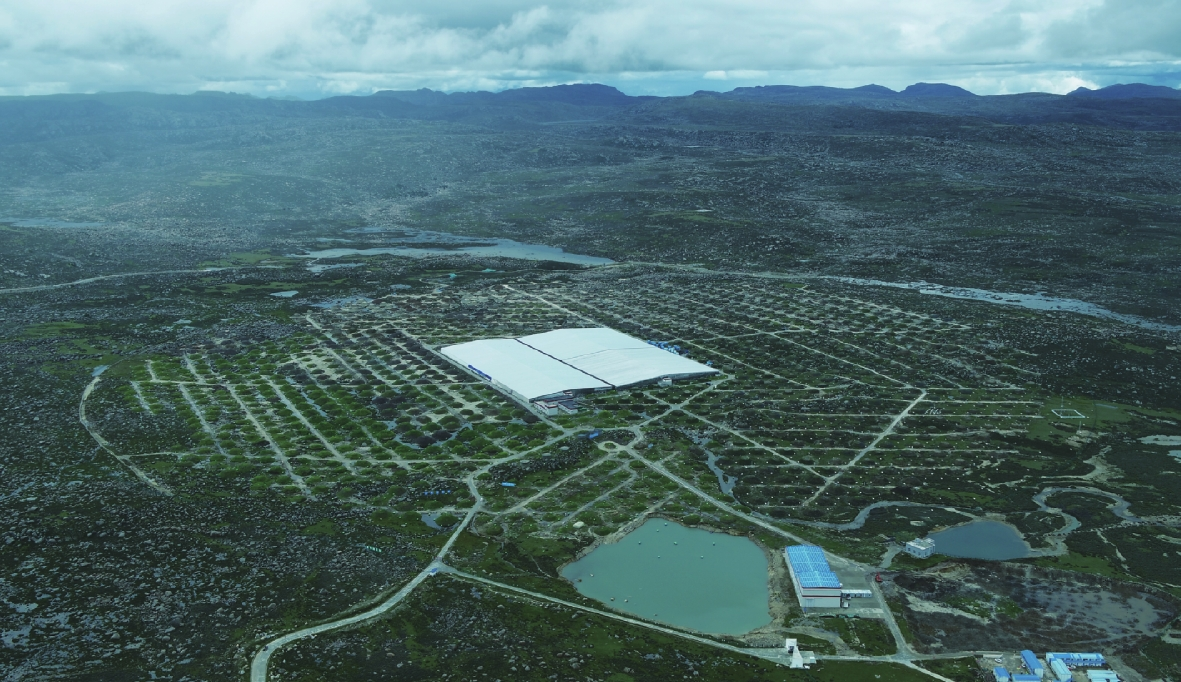
\includegraphics[height=0.15\textheight]{05_Astronomy/Images/telescopes/LHAASO.jpg}
    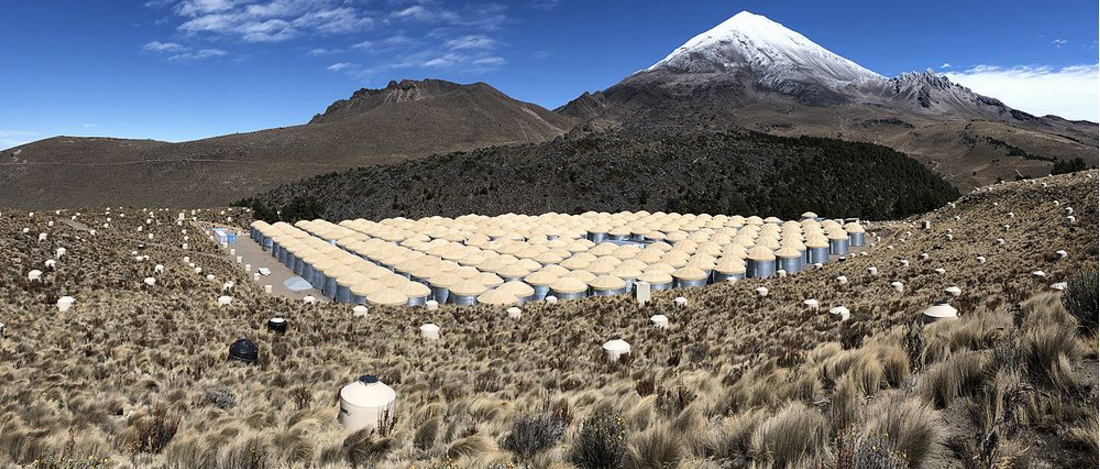
\includegraphics[height=0.15\textheight]{05_Astronomy/Images/telescopes/HAWC.png}
    \caption{The LHAASO (\textit{left}) and HAWC (\textit{right}) observatories. Images courtesy of \cite{2022ChPhC..46c0001M} and \cite{2023NIMPA105268253A}}
    \label{fig:my_label}
\end{figure}
\begin{itemize}
    \itemsep0em
    \item $1.3~\si{\kilo\meter\squared}$ array of $\approx 5200$ electromagnetic detectors and muon detectors that focuses on detecting gamma rays above $30~\TeV$ and cosmic rays from $10~\TeV$ to $100~\PeV$ \citep{2021ChPhC..45b5002A}.
    \item A water Cherenkov array sensitive to gamma rays between $100~\GeV$ and $30~\TeV$ and has total detection area of $7.8\times 10^4~\si{\meter\squared}$. This array monitors galactic gamma-ray sources, gamma-ray bursts and AGNs \citep{2021arXiv210103508L}.
    \item 18 Cherenkov telescopes that aims to measure the cosmic-ray energy spectrum and composition between $10~\TeV$ and $1~\si{E\electronvolt}$ \citep{2021EPJC...81..657A}.
    \item An upcoming electron-neutron detector array to study the cosmic-ray spectrum and composition above $1~\PeV$ \citep{2022ChPhC..46c0001M}.
\end{itemize}
\par~\par
LHAASO has detected significant gamma-ray emission above $100~\TeV$ from 12 Galactic sources including \mbox{LHAASO\,1825-1326} (LHAASO equivalent of \mbox{HESS\,J1825-137} / \mbox{HESS\,J1826-130}, see \autoref{fig:chapter1_hess_j1825_137_object_positions}) \citep{2021Natur.594...33C}. In 2021, LHAASO revealed the detection of gamma rays up to $1.1~\PeV$ from the Crab Nebula, implying the existence of a $2.3~\PeV$ electron \citep{doi:10.1126/science.abg5137}

\subsection{HAWC}

The High Altitude Water Cherenkov Observatory (HAWC) is a gamma-ray and cosmic-ray observatory located in Puebla, Mexico. The primary detector of HAWC consists of $300$ water tanks arranged in a $22\,000~\si{\meter\squared}$ area at an altitude of $\approx 4100~\m$ above sea level \citep{2023NIMPA105268253A}. The high refractive index of water ($n=1.33$) lowers the cosmic-ray/gamma-ray energy threshold to produce Cherenkov light which is then observed by four photomultiplier tubes.
\par~\par
HAWC has detected over $100$ sources of VHE gamma rays, which are summarised in the third HAWC catalogue \citep{2020ApJ...905...76A}. \cite{PhysRevLett.124.021102} revealed $9$ gamma-ray sources with emission above $56~\TeV$, with three of these sources having significant detection above $100\TeV$. This includes the equivalent \mbox{HESS\,J1825-137} / \mbox{HESS\,J1826-130}: \mbox{eHWC\,J1825-134}.

\subsection{The Cherenkov Telescope Array}

\begin{figure}[ht]
    \centering
    \includegraphics[width=0.9\textwidth]{05_Astronomy/Images/telescopes/cta_image.jpg}
    \caption{Telescopes for the Cherenkov Telescope Array. From left to right: the Small-Sized Telescope, two of the proposed Middle-Sized Telescope and the Large-Size Telescope. Image courtesy of \cite{cherenkov_telescope_array}.}
    \label{fig:chapter_2_cta}
\end{figure}

The Cherenkov Telescope Array (CTA) is the next generation ground-based telescope array that will observe gamma rays from $10~\GeV$ up to $300~\TeV$. It will be the largest ground-based telescope that can observe the night sky with sensitivity up to $10$ times greater than current instruments (see \autoref{fig:chapter_2_sensitivity comparison}). CTA will have two arrays in both the Southern (Chile) and Northern hemisphere (Canary Islands) to allow access to the majority of the night sky.
\par~\par
CTA will be an array of three different sized telescopes (see \autoref{fig:chapter_2_cta}): Small-Sized Telescopes (sensitive to energies $>1~\TeV$) with a mirror diameter and field of view of $4~\m$ and $\approx\ang{0}$ respectively, Medium-Sized Telescopes (sensitive to energies between $80~\GeV$ and $50~\TeV$) with a mirror diameter and field of view of $11.5~\m$ and $\approx\ang{7.5}$ respectively and the Large-Sized Telescope (sensitive to the lowest energy gamma rays) with a mirror diameter and field of view of $\approx 23~\m$ and $\approx\ang{4.3}$ respectively \citep{cherenkov_telescope_array,2019scta.book.....C}.
\par~\par
PWN transitioning from their second to their third stage of evolution (see \autoref{sec:01_intro_time_ev_PWN}) are too faint and/or extended for their emission to be detected by current instruments such as H.E.S.S.. The increased sensitivity of CTA (see \autoref{fig:chapter_2_sensitivity comparison}) will be able observe these previously undetectable $\TeV$ PWN, providing more insight into the evolution of PWN.
\chapter[ISM towards \mbox{HESS\,J1825-137} and \mbox{HESS\,J1826-130}]{Interstellar Medium towards \\ \mbox{HESS\,J1825-137} and \mbox{HESS\,J1826-130}} \label{06_ISM}

\begin{wrapfigure}[31]{R}{0.45\textwidth}
	\centering
	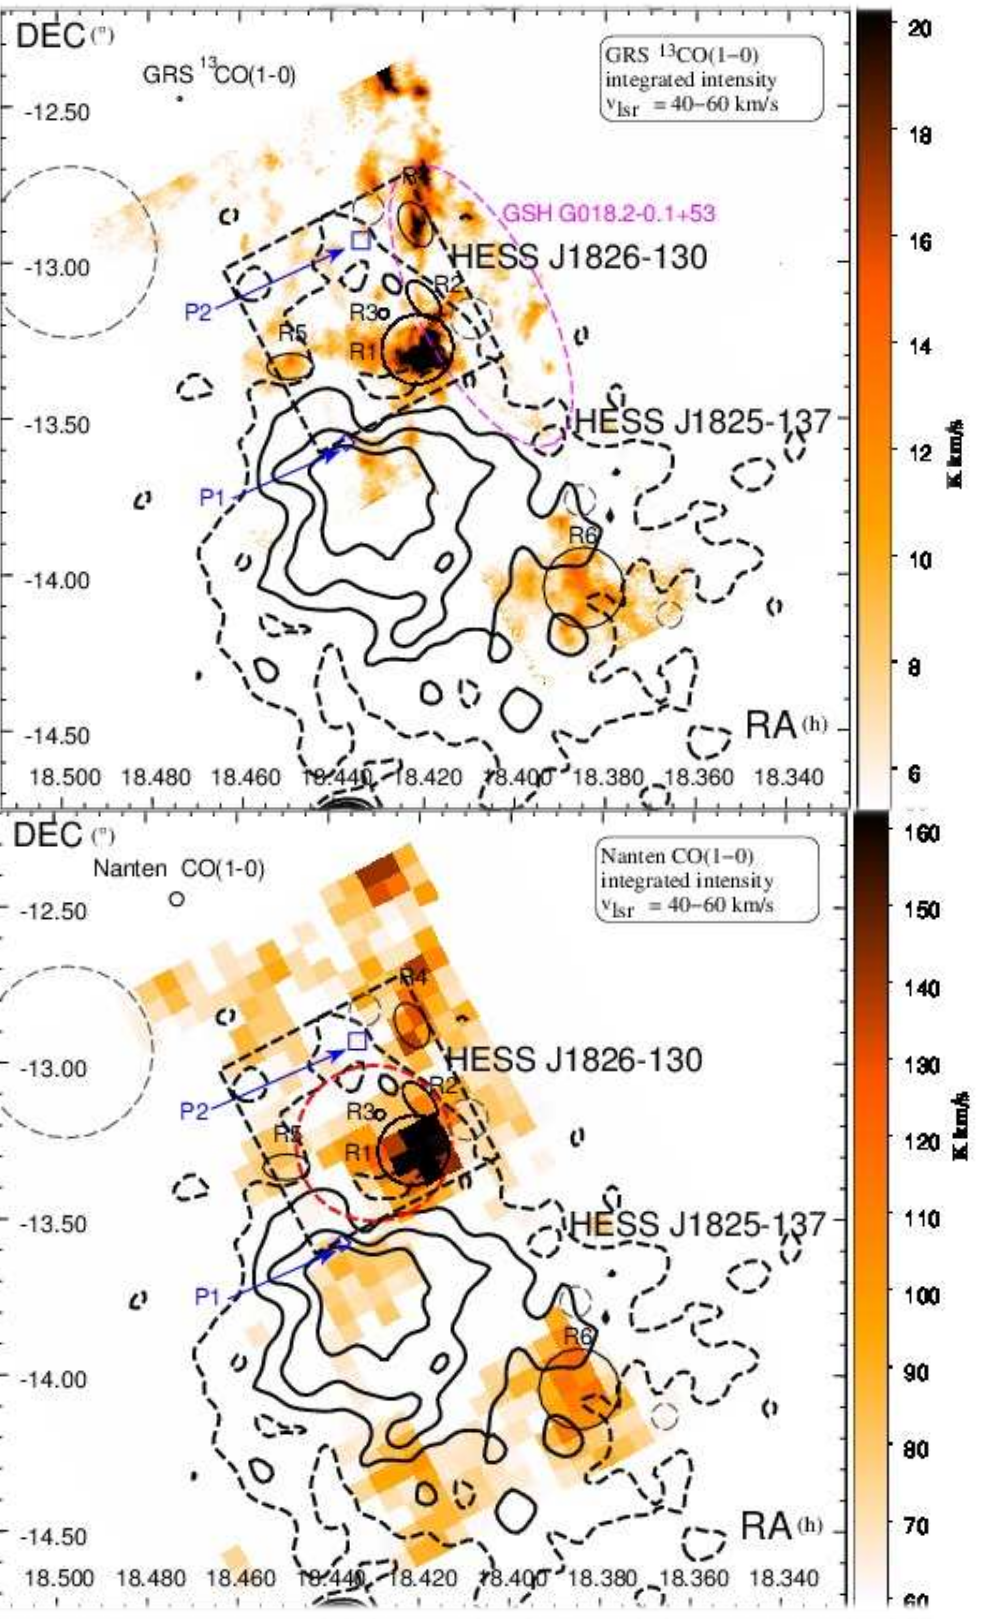
\includegraphics[width=0.45\textwidth]{06_Interstellar_Medium/Images/18252.png}
    \caption{$^{13}$CO$\qty(1-0)$ (\textit{top}) and $^{12}CO\qty(1-0)$ (\textit{bottom}) integrated intensity between velocity range $40-60~\si{\kilo\meter\per\second}$ (equivalent to $3.5-4.5~\kpc$) towards \mbox{HESS\,J1825-137}. HESS TeV gamma-ray emission contours are shown by the solid and dashed black contours. Image courtesy of \citep{2016MNRAS.458.2813V}}
	\label{fig:chapter_6_1825_gas}
\end{wrapfigure}

The interstellar medium (ISM) is the gas existing in between stars and other astrophysical objects in the Galaxy. The ISM includes atomic and molecular gas, dust, plasma and cosmic rays and accounts for $10-15\%$ of the total mass in the Galactic disc \citep{2001RvMP...73.1031F}. By number, the chemical composition of the ISM is $90.8\%$ hydrogen, $9.1\%$ helium and $0.12\%$ heavier elements \citep{2001RvMP...73.1031F}. By mass hydrogen makes up $70.4\%$ of the ISM with the remainder being $28.1\%$ Helium and $1.5\%$ heavier elements. As cosmic rays and gamma rays leave their place of birth, they must traverse the ISM before being observed at Earth.
\par~\par 
As discussed in \autoref{sec:01_1825_1826}, \mbox{HESS\,J1825-137} lies at a distance of $4.0~\kpc$  \citep{2006A&A...460..365A}. \autoref{fig:chapter_6_1825_gas} shows carbon monoxide (CO) gas lying in range $3.5-4.5~\kpc$ towards \mbox{HESS\,J1825-137} and \mbox{HESS\,J1826-130}, where CO is used as a trace for molecular hydrogen (see \autoref{sec:06_molecular_tracers}). The ISM gas towards this region will influence the transport of cosmic rays escaping the PWN (and SNR) associated with \mbox{HESS\,J1825-137} and the subsequent gamma-ray emission from this region. Therefore the ISM must be considered in any study towards this region. This chapter will discuss properties of the ISM as well as the observatories whose data products were used in this thesis.
\newpage  %I need to put this or elese it looks nasty (due to the wrap figure)
\section{Detecting the interstellar medium}

The ISM gas towards \mbox{HESS\,J1825-137} influences the rate at which cosmic rays propagate and their cooling time (see \autoref{sec:chapter1_non_thermal_emission}). Radiation theory describes how particles (photons and cosmic rays) interact with a medium during propagation \citep{2011piim.book.....D}. As photons travel through the ISM before detection at Earth, it is important to characterise how the interstellar gas affects observations.

\subsection{Specific Intensity, Specific Flux and Bolometric flux}

Firstly, this section will define fundamental concepts.
\par~\par 
\noindent Let a telescope with detecting area $\dd{A}$ observe photons (in frequency range $\nu + \dd{\nu}$ and energy range $E+\dd{E}$) from a source within solid angle $\dd{\Omega}$ at orientation $\theta$ in time $\dd{t}$ (see \autoref{fig:telescope_basic_diagram2}).

\begin{SCfigure}[0.42][h!]
	\centering
	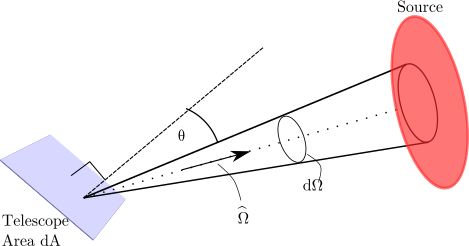
\includegraphics[width=0.7\textwidth]{06_Interstellar_Medium/Images/Theory/intensity.png}
	\caption{A basic illustration of a telescope with area $\dd{A}$ observing a cloud of ISM gas with solid angle $\dd{\Omega}$ at at orientation $\theta$.}
	\label{fig:telescope_basic_diagram2}
\end{SCfigure}
\noindent The amount of photons arriving within solid angle $\dd{\Omega}$ is described by the the specific intensity:

\begin{equation}
	\begin{aligned}
		I_\nu\qty(\hat{\Omega})&=\frac{\dd{E}}{\dd{A}\dd{t}\dd{\nu}\dd{\Omega}}\quad\qty[\si{\watt\per\meter\squared\per\hertz\per\steradian}]\text{ .}
	\end{aligned}
\end{equation}
% \noindent Alternative units for specific intensity are $\si{\erg\per\second\per\centi\meter\squared\per\hertz\per\steradian}$.
\par~\par 
\noindent The net specific flux, $F_\nu$, is obtained by integrating the specific intensity over the entire source:

\begin{equation}
	\begin{aligned}
		F_\nu &=\oint I_\nu\qty(\hat{\Omega})\cos\theta\dd{\Omega}\quad\qty[\si{\watt\per\meter\squared\per\hertz}]\text{ .}
	\end{aligned}
\end{equation}
\noindent A common unit for the specific flux in the radio domain is the Janksy ($\si{Jy}$) where $1~\si{Jy}=10^{-26}~\si{\watt\per\meter\squared\per\hertz} = 10^{-23}~\si{\erg\per\centi\meter\squared\per\second\per\hertz}$. If the specific intensity is isotropic ($I_\nu\qty(\hat{\Omega})=I_\nu$) then $\oint \cos\theta\dd{\Omega}=0$ and the specific flux is zero. If the telescope is pointed towards the source ($\cos\theta=1$) and the source is uniformly bright ($I_\nu\qty(\hat{\Omega})=I_\nu$), then the specific flux is simply:
\begin{equation}
	\begin{aligned}
		F_\nu&=I_\nu\Delta\Omega\text{ .}
	\end{aligned}\label{eq:specifc_flux_uniform_source}
\end{equation}
\noindent The bolometric flux, $F$, is the specific flux integrated over all frequencies:

\begin{equation}
	\begin{aligned}
		F&=\int F_\nu \dd{\nu}~\quad\qty[\si{\watt\per\meter\squared}]\text{ ,}
	\end{aligned}
\end{equation}
\noindent and is a measure of the total amount of photons emitted by a source.

\subsection{Radiative Transfer}

Let a cloud with thickness $\dd{s}=c\dd{t}$ (volume $\dd{V}=\dd{A}c\dd{t}$) and particle number density $n$ be illuminated by a background source with specific intensity $I_\nu$ on area $\dd{A}$ (see \autoref{fig:photon_energy_density}).

\begin{figure}[H]
	\centering
	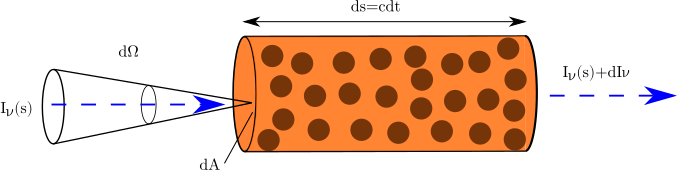
\includegraphics[width=\textwidth]{06_Interstellar_Medium/Images/Theory/radiative_transfer.png}
	\caption{A cloud of thickness $\dd{s}$ is illuminated by a background source with intensity $I_\nu\qty(s)$. Photons of frequency $\nu$ are emitted and re-emitted by particles (dark circles) within the cloud, changing the intensity by $\dd{I_\nu}$}
	\label{fig:photon_energy_density}
\end{figure}
\noindent The cloud contains $n\dd{V}$ particles with each particle having an absorption cross section $\sigma_\nu$ for radiation of frequency $\nu$. The total absorption area of the cloud can be described by $n\dd{s}\dd{A}\sigma_\nu$, giving the fraction of photons absorbed to be:

\begin{equation}
    \begin{aligned}
        f_\text{absorbed}&=n\dd{s}\dd{A}\sigma_\nu/\dd{A} \\
        &=n\dd{s}\sigma \text{ .}
    \end{aligned}
\end{equation}
\noindent Therefore the change in intensity due to absorption is:

\begin{equation}
    \begin{aligned}
        \dd{I_{\nu,\text{absorbed}}}&=- \frac{n\dd{V}\sigma_\nu}{\dd{A}} \\
        &= - \alpha_\nu I_\nu \dd{s}\text{ ,}
    \end{aligned}
\end{equation}
\noindent where $\alpha_\nu=n\sigma_\nu~\qty[\si{\per\meter}]$ is the absorption coefficient. The absorption mean free path is the distance a photon will travel in the cloud before absorption and is given by:

\begin{equation}
	\begin{aligned}
		\ell_\nu &=\alpha_\nu^{-1}\text{ .}
	\end{aligned}
\end{equation}

\noindent If the cloud in \autoref{fig:photon_energy_density} has emission emission coefficient $j_\nu$
$\qty[\si{\watt\per\meter\cubed\per\hertz\per\steradian}]$ (i.e. the power emitted at frequency $\nu$ by an infinitesimal volume $\dd{V}$), the specific intensity emitted by the cloud is:

\begin{equation}
	\begin{aligned}
		\dd{I_{\nu\text{, emitted}}}&=j_\nu \dd{s} \\
		\therefore I_{\nu\text{, emitted}} &= \int j_\nu \dd{s} \text{ .}
	\end{aligned}\label{eq:emission_coefficient}
\end{equation}
\noindent Giving the total change in intensity in the cloud to be:

\begin{equation}
	\begin{aligned}
		\dv{I_\nu}{s}&=-\alpha\qty(s)I_\nu\qty(s)+j_\nu\qty(s) \\
		\frac{\dd{I_\nu}}{\alpha_\nu\dd{s}}&=-I_\nu\qty(s)+\frac{j_\nu\qty(s)}{\alpha_\nu\qty(s)} \\
		\dv{I_\nu}{\tau}&=-I_\nu\qty(\tau_\nu)+S\qty(\tau_\nu)\text{ ,}
	\end{aligned} \label{eq:radiative_transfer}
\end{equation}
\noindent where $\tau_\nu$ is the optical depth defined by:

\begin{equation}
	\begin{aligned}
		\dd{\tau_\nu}&=\alpha_\nu \dd{s}\text{ ,}
	\end{aligned}
\end{equation}
\noindent and $S_\nu\qty(\tau_\nu)=j_\nu\qty(s)/\alpha_\nu\qty(s)$ is the source function of the cloud. \autoref{eq:radiative_transfer} has solution:

\begin{equation}
	\begin{aligned}
		I_\nu\qty(\tau_\nu)&=\exp\qty(-\tau_\nu)\qty[I_\nu\qty(0)+\int_{0}^{\tau_\nu}\exp\qty(\tau'_\nu)S_\nu\qty(\tau'_\nu)\dd{\tau'_\nu}] \text{ .}
	\end{aligned} \label{eq:radiative_transfer_solution1}
\end{equation}

If there is no emission from the cloud, $S_\nu\qty(\tau_\nu)=j_\nu\qty(s)=0$, then the specific intensity can be described by:

\begin{equation}
    \begin{aligned}
        I_\nu\qty(\tau_\nu)&=I_\nu\qty(0)\exp\qty(-\tau_\nu)\text{ .}
    \end{aligned}
\end{equation}
\noindent i.e. the specific intensity of the background source after absorption by the cloud. If the emission/absorption of the cloud is uniform, $S_\nu\qty(\tau_\nu)=S_\nu$, \autoref{eq:radiative_transfer_solution1} becomes:

\begin{equation}
	\begin{aligned}
		I_\nu\qty(\tau_\nu)&=I_\nu\qty(0)\exp\qty(-\tau_\nu)+S_\nu\qty(1-\exp\qty(-\tau_\nu)) \\
        &=S_\nu + \exp\qty(-\tau_\nu)\qty[I_\nu\qty(0)-S_\nu] \text{ .}
	\end{aligned} \label{eq:radiative_transfer_solution2}
\end{equation}
\noindent If optically thick, $\tau_\nu\gg 1$:

\begin{equation}
    \begin{aligned}
        I_\nu\qty(\tau_\nu)&\approx S_\nu\text{ .}
    \end{aligned}
\end{equation}
\noindent This is when a medium is opaque and only photons emitted by the cloud are observed. If optically thin, $\tau \ll 1$, then the exponential in \autoref{eq:radiative_transfer_solution2} can be approximated by $\exp(-\tau_\nu)\approx 1-\tau_\nu$ and the observed specific intensity becomes:

\begin{equation}
	\begin{aligned}
		I_\nu\qty(\tau_\nu)&=I_\nu\qty(0)\qty(1-\tau_\nu)+S_\nu\tau_\nu\text{ .}
	\end{aligned}
\end{equation}

\subsection{Black Bodies} \label{sec:06_blackbodies}

Thermal radiation is the emitted radiation due to the random motion/kinetic energy (i.e. temperature) of its particles. Thermal sources such as stars, CMB, interstellar dust can be described by an object emitting radiation with frequency $\nu$ at temperature $T$. A black body is an idealised object that absorbs all incoming radiation. A black body at temperature $T$ emits radiation at an intensity described by Planck's distribution:

\begin{equation}
	\begin{aligned}
		B_\nu\qty(T)&= \frac{2h\nu^3/c^2}{\exp(h\nu/kT)-1}\quad\qty[\si{\watt\per\steradian\per\meter\squared\per\hertz}] \text{ ,}
	\end{aligned}
\end{equation}
\noindent  where $h$ is Planck's constant and $k$ is Boltzmann's constant. The integrated intensity over all frequencies from a black body is given by the Stefan-Boltzman Law:

\begin{equation}
	\begin{aligned}
		F&=\sigma T^4~\qty[\si{\watt\per\meter\squared}]\text{ ,}
	\end{aligned}
\end{equation}
\noindent with $\sigma$ being the Stefan–Boltzmann constant. Objects in thermal equilibrium emit radiation in a manner that is dependent on their temperature. For an `ideal' black body to be in thermal equilibrium with its surroundings, the incoming intensity ($I\qty(0)=B_\nu$) and emitted intensity ($I\qty(\tau)=B_\nu$) are equal. \autoref{eq:radiative_transfer_solution2} becomes:

\begin{equation}
    \begin{aligned}
        B_\nu\qty(T)&=S_\nu\qty(T) + \exp\qty(-\tau_\nu)\qty[B\qty(T)-S_\nu\qty(T)] \text{ .}\\
    \end{aligned}
\end{equation}
\noindent This is only true for all $\tau$ when:

\begin{equation}
    \begin{aligned}
    	\therefore S_\nu\qty(T) &= B_\nu\qty(T)=\frac{j_\nu\qty(T)}{\alpha_\nu\qty(T)}\text{ .}
    \end{aligned} \label{eq:kirchoffs_law}
    \end{equation}
\noindent \autoref{eq:kirchoffs_law} is known as Kirchoff's law of radiation. Hence, the emission of a black body can be described by:

\begin{equation}
    \begin{aligned}
        I_\nu\qty(\tau_\nu)&=I_\nu\qty(0)\exp(-\tau_\nu)+B_\nu\qty(T)\qty[1-\exp(-\tau_\nu)]\text{ .}
    \end{aligned} \label{eq:chapter_6_black_body_emission}
\end{equation}
\noindent For an optically thick medium ($\tau\gg 1$) then:

\begin{equation}
    \begin{aligned}
        I_\nu\qty(\tau_\nu)\approx B_\nu\qty(T) \text{ ,}
    \end{aligned}
\end{equation}
\noindent and the medium can be approximated as a black body. Molecular tracers such as CO (see \autoref{sec:06_molecular_tracers}) emit radiation in the radio band. At these low frequencies ($h\nu\ll kT$ and $\exp(h\nu/kT)\approx1+h\nu/kT$) , the intensity of a black body can be approximated by:

\begin{equation}
    \begin{aligned}
        B_\nu\qty(T)&=\frac{2\nu^2kT}{c^2}\text{ .}
    \end{aligned}
\end{equation}

In radio astronomy, brightness temperature ($T_B$) is often used to measure intensity where $B_\nu(T_B)\equiv I_\nu$:

\begin{equation}
    \begin{aligned}
        T_B\qty(\nu)&=\frac{c^2}{2\nu^2 k}I_\nu\text{ .}
    \end{aligned} \label{eq:chapter_6_brightness_temp}
\end{equation}
\noindent Brightness temperature is the temperature that an ideal black body in thermal equilibrium would have in order to emit intensity $I_\nu$. For example, brightness temperature can be used to describe molecular clouds with temperatures $\approx 10~\si{K}$ for frequencies $\ll 208~\si{\giga\hertz}$ \citep{2011hea..book.....L}.

\subsection{Spectral Line Excitation and Emission} \label{sec:interstellar_medium_excitation_emission}

\begin{figure}[h]
	\centering
	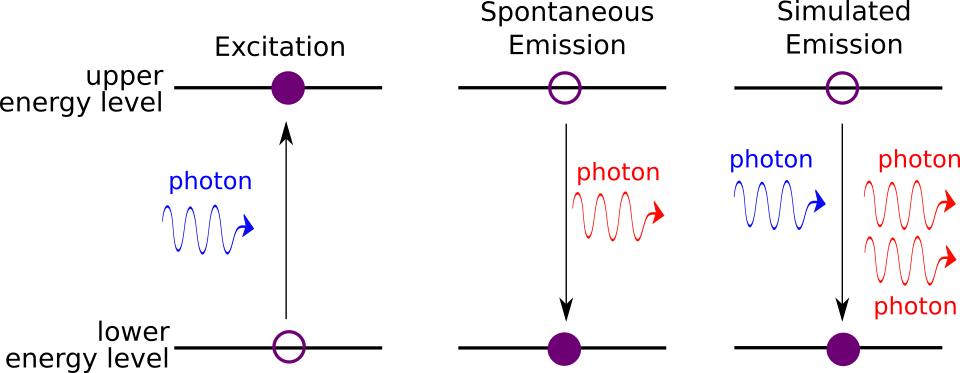
\includegraphics[width=0.7\textwidth]{06_Interstellar_Medium/Images/Theory/emission.png}
	\caption{(\textit{left}) Excitation of an electron from a low to higher energy level due to absorption of energy from a photon. (\textit{middle}) Spontaneous emission of a photon with energy equal to energy difference between energy levels. (\textit{right}) Simulated emission of a photon with same wavelength and direction as incident photon.}
	\label{fig:absorption_emission}
\end{figure}

Atoms populate their electrons in orbitals, from low to high energy levels. The stable state (or ground state) of an atom occurs when the electrons occupy their lowest energy level. The absorption of a photon can raise the energy level of an atom to a higher one (see left panel of \autoref{fig:absorption_emission}). This is known as excitation. An atom can exist in this excited state for a short period of time until it decays to a lower energy level and emits a photon with energy equal to the energy difference between the initial and final energy level (see middle panel if \autoref{fig:absorption_emission}). This is known as spontaneous emission. The Einstein coefficient, $A_{if}$, gives the probability per unit time for spontaneous emission from state $i$ to state $f$ and releasing photon of frequency $\nu_{if}$. If the number density of atoms in state $i$ is $n_i$, then the emission coefficient is given by:

\begin{equation}
	\begin{aligned}
		j_\nu&=\frac{n_ih\nu_{if}A_{if}}{4\pi}\Phi\qty(\nu)\text{ .}
	\end{aligned} \label{eq:interstellar_medium_emission_coefficient}
\end{equation}


For example, H$\alpha$ emission occurs when the electron in an excited hydrogen atom decays from the third to second energy level. As a result H$\alpha$ emission is used as a tracer for ionised gas. In its neutral state, a hydrogen atom consists of one electron-proton pair with their spins either parallel or anti-parallel. The hydrogen atom may spontaneously switch the spin of its electron from parallel to anti-parallel to the proton spin and release radiation with a wavelength of $21~\cm$ known as the HI line. This HI line can be used to probe neutral hydrogen gas in the Galaxy and beyond.
\par~\par
Simulated emission occurs when an external photon interacts with an excited atom causing an emission of a photon with the same wavelength, polarisation and direction as the initial photon (see \autoref{fig:absorption_emission}).

\section{Probing the interstellar medium} 

\subsection{Molecular Tracers} \label{sec:06_molecular_tracers}

H$_2$ is the most abundant molecule in the Galaxy, consisting of two bound hydrogen atoms. Molecular hydrogen has 14 vibration energy levels that require high temperatures ($>5000~\si{\kelvin}$) for excitation \citep{2011piim.book.....D}. However, observed molecular clouds have temperatures $\approx 10-20~\si{\kelvin}$ \citep{2001RvMP...73.1031F} and the transition rate to higher energy levels are quite low. Moreover, the symmetry of H$_2$ molecules makes dipole radiation `forbidden' while electric quadruple radiation is possible with very low probability \citep{2011piim.book.....D}.
\par~\par 
The two nuclei in $H_2$ molecules rotate around their centre of mass with angular momentum components $J_x$, $J_y$ and $J_z$ \citep{alma99117570501811} and total rotational energy:

\begin{equation}
    \begin{aligned}
        E_\text{rot}&=\frac{J_x^2}{2I_x}+\frac{J_y^2}{2I_y}+\frac{J_z^2}{2I_z}\text{ ,}
    \end{aligned} \label{eq:chapter_6_molecular_rotation_energy}
\end{equation}
\noindent where $I_{i}$ is the moment of inertia in the ith axis ($i=x,y,z$). For linear rotors (e.g. H$_2$, CO)  $I_x\ll I_y=I_z$ where $I_x$ can be treated as zero \citep{alma9928060792901811}. \autoref{eq:chapter_6_molecular_rotation_energy} becomes:

\begin{equation}
    \begin{aligned}
        E_\text{rot}&=\frac{J^2}{2I}\text{ ,}
    \end{aligned}
\end{equation}
\noindent where the eigenvalue of $J^2$ is $j\qty(j+1)\hbar^2$ \citep{alma99117570501811}. Hence:

\begin{equation}
    \begin{aligned}
        E_\text{rot}&=\frac{\hbar^2}{2I}j\qty(j+1)\text{ ,}
    \end{aligned}
\end{equation}
\noindent with $\hbar=h/\qty(2\pi)$ and $j=0$, $1$, $2$... For a $H_2$ molecule absorbing/emitting a photon (with energy $E_\gamma$) that causes a change in energy level, the difference in energy levels is given by:

\begin{equation}
    \begin{aligned}
        E_\gamma=\Delta E_{rot} = \frac{j\hbar^2}{I}\text{ .}
    \end{aligned}
\end{equation}
\noindent For molecular hydrogen, temperatures greater than $100~\si{\kelvin}$ are required for rotational energy excitation. Hence, molecules within the majority of quiescent $H_2$ clouds exist in their vibrational and rotational ground state. 
\par~\par 
After H$_2$, the second most abundant molecule is CO, following a  CO/H$_2$ abundance ratio of $10^{-4}$ in molecular clouds \citep{1994ApJ...428L..69L}. The transition between the ground and first rotational energy level ($J=1-0$) for CO requires much lower temperatures $\approx 5~\si{\kelvin}$, corresponding to photons being emitted at frequency $115~\si{\giga\hertz}$ ($\lambda=2.6~\si{\milli\meter}$) \citep{alma9927598238601811}. Therefore, carbon monoxide can be used as a tracer for molecular hydrogen (see \citep{Bolatto2013}).
\par~\par
High-frequency radio telescopes such as Nanten (see \autoref{sec:NANTEN}) observe the intensity of molecular CO in units of brightness temperature (see \autoref{eq:chapter_6_brightness_temp}). To interpret the amount of gas towards a particular region, the CO$(1-0)$ brightness intensity is converted to a column density ($\si{\per\centi\meter\squared}$) of molecular hydrogen through the conversion factor $X_\text{CO}$:

\begin{equation}
	\begin{aligned}
		N_{H_2}&=X_\text{CO}W_\text{CO}\text{ ,}
	\end{aligned}
\end{equation}
\noindent where $W_\text{CO}$ is the integrated intensity in units $\si{\\kilo\meter\per\second}$. The conversion factor is often assumed to be constant ($X_\text{CO}=1.5\times 10^{20}~\si{\per\centi\meter\squared\per\kelvin\per\kilo\meter\squared\second}$) across the Galactic plane, but it is known to vary with galactocentric radius \citep{2004A&A...422L..47S}. The number density $n_H$ and mass $M_H$ of hydrogen in a cloud with column density $N_{H_2}$ are respectively:

\begin{equation}
	\begin{aligned}
		n_H&=\frac{\mu N_{H_2}}{\Delta z} \label{eq:06_density_gas} \\
		M_H&=n_Hm_pV\text{ ,}
	\end{aligned}
\end{equation}
\noindent $\Delta z$ is the width of the cloud along the line of sight, $V$ is the volume of the cloud and $m_p$ is the mass of the proton. The weight factor, $\mu$, of a gas cloud is:

\begin{equation}
    \begin{aligned}
        \mu&=\sum_Z n A_r\text{ ,}
    \end{aligned}
\end{equation}
\noindent where $\sum_Z$ sums over the molecules present in the cloud, $n$ is the number of atoms present in the molecule ($n=2$ for molecular hydrogen) and $A_r$ is the atomic weight ($A_r\approx1$ for hydrogen and $A_r\approx 4$ for helium). For a gas cloud with $20\%$ Helium component, the weight factor is $2.8$.

\subsection{Doppler Shift}

\autoref{sec:06_molecular_tracers} discussed how atomic and molecular gas emit photons with wavelengths dependent on their atomic structure. However, the bulk movement of gas clouds around the Galactic Center (GC) will shift the frequency of photons due to the Doppler effect. The shift in frequency is described by:

\begin{equation}
    \begin{aligned}
        \nu = \frac{c+V_\text{obs}}{c+V}\nu_0\text{ ,}
    \end{aligned}
\end{equation}
\noindent where $\nu$ is the observed frequency, $\nu_0$ is the emitted frequency, $V$ is the veloicty of the gas cloud and $V_\text{obs}$ is the velocity of the observer. Therefore, a shift in frequency can be represented as a velocity in respect to a rest frame:

\begin{equation}
    \begin{aligned}
        V_\text{LSR}=c\frac{\qty(\nu_0-\nu)}{\nu_0}\text{ .}
    \end{aligned}
\end{equation}
\noindent The typical rest frame used is the local standard of rest (LSR), taken at the point coincident with the Sun orbiting around the GC in a perfect circular orbit.

\subsection{Galactic Rotation Curve} \label{sec:06_galactic_rotation}

Matter rotates around the GC with an average tangential speed of $\Theta_0\approx 220~\kmpersec$. The Galactic rotation curve is an empirical model (see \autoref{fig:Galactic_rotation_model}) that relates the galactocentric radius (distance to the GC) of an object to its observational velocity.
\begin{figure}[h!]
	\centering
	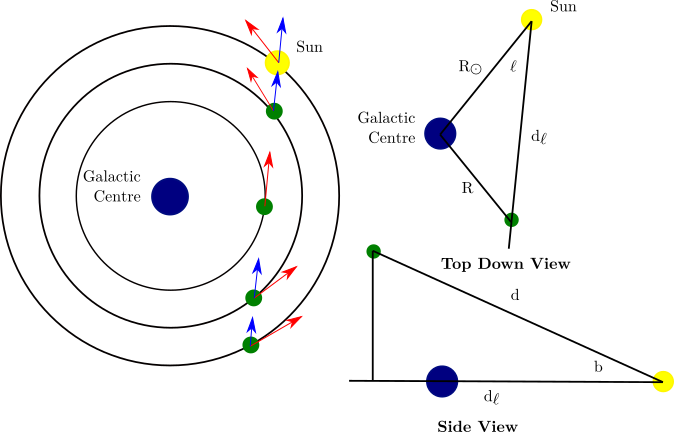
\includegraphics[width=1.0\textwidth]{06_Interstellar_Medium/Images/Theory/galaxy_combined.png}
	\caption{(\textit{Left}) Rotation of the Galaxy around the GC (dark blue circle) with the yellow circle as the Sun, the blue arrow is the tangential velocity of the green objects (e.g. gas cloud) and the blue arrows are their velocities projected along the line of sight to the Sun. (\textit{Right}) Geometry of an object at Galactic longitude $\ell$, Galactic latitude $b$ and distance $d$ from the Sun.}
	\label{fig:Galactic_rotation_model}
\end{figure}
Using HI clouds, \cite{1993A&A...275...67B} found that the measured velocity of a cloud, $V_\text{LSR}$, can be transformed into circular rotation velocity, $\Theta_0$ via:
\begin{equation}
\begin{aligned}
    V_\text{LSR}&=\qty(\frac{\Theta R_\odot}{R}-\Theta_\odot)\sin\ell \cos b\text{ ,}
\end{aligned} \label{eq:chapter_6_brand_blitz_velocity}
\end{equation}
\noindent where $\ell$ and $b$ are the Galactic coordinates of the cloud, $R$ and $\Theta$ are the galactocentric distance and circular rotation velocity velocity of the cloud respectively and $R_\odot$ is the galactocentric distance of the Sun. The circular rotation velocity is related to the galactocentric distance by:

\begin{equation}
    \begin{aligned}
        \frac{\Theta}{\Theta_\odot}&=a_1 \qty(\frac{R}{R_\odot})^{a_2}+a_3\text{ ,}
    \end{aligned} \label{eq:06_circular_rotatoin_velocity}
\end{equation}
\noindent where $a_1=1.00767$, $a_2=0.0394$ and $a_3=0.00712$ are the values found by \cite{1993A&A...275...67B}. For a cloud with circular rotation velocity $V_\text{LSR}$ at coordinate $\ell$ and $b$, \autoref{eq:chapter_6_brand_blitz_velocity} and \autoref{eq:06_circular_rotatoin_velocity} can be solved numerically to find $R$ and $\Theta$. Using simple trigonometry (see \autoref{fig:Galactic_rotation_model}), the distance to the GC for an object at distance $d$ and coordinates $\qty(\ell,b)$ is given by:

\begin{equation}
    \begin{aligned}
        R^2&=d^2\cos^2b+R_\odot^2-2dR_\odot\cos b\cos\ell\text{ ,}
    \end{aligned}
\end{equation}
\noindent which gives a near and far distance to the cloud (see \autoref{fig:Galactic_rotation_model}). In general, the near distance is taken to be the solution; a source further away is more likely to have its emission being obstructed by closer gas. Moreover, a distant source will appear dimmer than a nearby source due to intensity following the inverse square law ($I\propto d^{-2}$).
\par~\par 
Other Galactic rotation curves include \cite{1985ApJ...295..422C}, who analysed the Massachusetts-Stony Brook Galactic plane CO survey \citep{1985ApJ...289..373S}. \cite{1996MNRAS.281...27P} provided a `universal rotation curve' which includes contributions from a stellar disk and a dark halo. Alternatively \cite{2014ApJ...783..130R} describes the Galactic rotation curve as a polynomial:

\begin{equation}
    \begin{aligned}
        \Theta\qty(R)&=a_{p1}+a_{p2}\rho+a_{p3}\rho^3 \\
        \rho &=\frac{R}{R_0}-1\text{ ,}
    \end{aligned}
\end{equation}
\noindent with $a_{p1}=[241\pm 9]~\kmpersec$, $a_{p2}=0.5\pm 3.7$ and $a_{p3}=-15.1\pm 8.4$. 
\par~\par 
The velocity in \autoref{eq:chapter_6_brand_blitz_velocity} describes the circular rotation velocity of an object around the Galaxy. However, the velocity measured at Earth is the combined velocity due to Galactic rotation and local individual gas motion (e.g. due to stellar winds, SNR shock fronts). \cite{1993A&A...275...67B} noted that residuals of modelled gas with respect to the Galactic rotation curve can be as large as $40~\kmpersec$ with the average being around $12.8~\kmpersec$. This is significant compared to the Nanten observatory velocity resolution of $1~\kmpersec$ (see \autoref{sec:NANTEN}), whose data products were used in this thesis. The uncertainty in the individual velocity of the gas will lead to large uncertainties in distances (hundreds of parsecs) to gas clouds.
\par~\par 
\begin{figure}
    \centering
    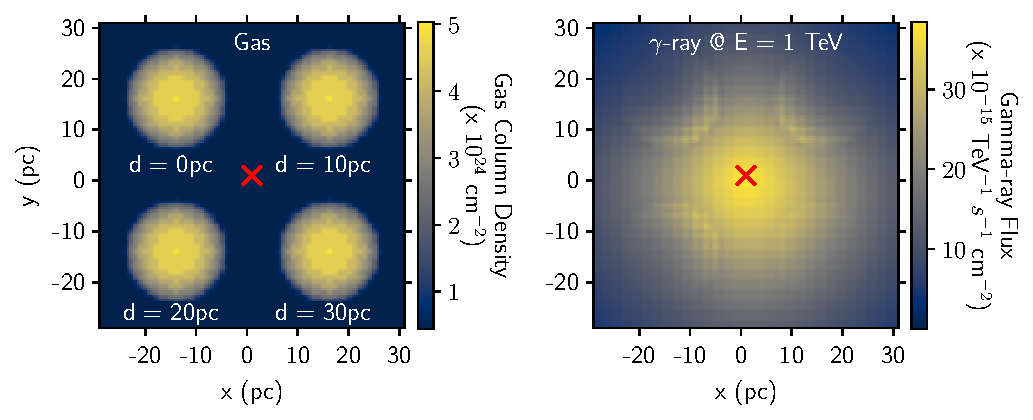
\includegraphics[width=1.0\textwidth]{06_Interstellar_Medium/Images/Theory/gas_distance_example.pdf}
    \caption{(\textit{Left}) Four spherical gas clouds located $4~\kpc$ from the Earth at distances $d$ along the line of sight (z-axis runs in/out of page) from a source of electrons (red cross). (\textit{Right}) Subsequent gamma-ray flux $40~\kiloyear$ after electron injection commences.}
    \label{fig:06_gas_distance_Example}
\end{figure}
The large uncertainties in distances to gas clouds (see \autoref{sec:06_galactic_rotation}) leads to a caveat in modelling the gas and magnetic field distribution (see next section) around a cosmic ray source. For example, consider a crude estimation in which the cosmic ray intensity is described by an inverse square law $I\propto d^{-2}$ where $d$ is the distance from the accelerator. The cosmic ray flux decreases with distance from a source, decreasing the subsequent gamma ray energy flux from non-thermal emission (see \autoref{sec:chapter1_non_thermal_emission}). This can be seen in \autoref{fig:06_gas_distance_Example}, where four spherical gas clouds of number density $600~\centimeterminusthree$ ($B\approx 25~\si{\micro G}$) are located at different distances along the line of sight (z-axis) from a continuous source of electrons. The gamma-ray flux through IC interactions at $40~\kiloyear$ (suggested age of PWN \mbox{HESS\,J1925-137}, \cite{2011ApJ...742...62V}) decreases with increasing distance from the accelerator. Therefore, large uncertainties in distances to gas clouds will influence the modelled multiwavlength emission towards an accelerator.

\subsection{Magnetic fields in molecular clouds} \label{eq:sec_Bfield_gas}

The Zeeman effect (the splitting of spectral lines in the presence of a static magnetic field) can be used to measure the magnetic field strength in a medium. \cite{2010ApJ...725..466C} studied a population of quiescent clouds and related the magnetic strength a cloud's its number density $n$ through:

\begin{equation}
    \begin{aligned}
        B_\text{gas}\qty(n)=
    \begin{cases}
        B_0 \qquad &\text{, } n < n_0 \\
        B_0\qty(\frac{n}{n_0})^\alpha \qquad &\text{, } n > n_0
    \end{cases}\text{ ,}
    \end{aligned} \label{eq:ISM_crutchers}
\end{equation}
\noindent where clouds with a density above $n_0=300~\centimeterminusthree$ have an enhanced magnetic field described by a power-law regime with $B_0=10~\si{\micro G}$ and $\alpha=0.65$.
\par~\par 
Cosmic rays propagating through the ISM scatter off magnetic field turbulence and the overall motion is described by a random walk/diffusion (see \autoref{chapter_1_cr_propagation}), where the rate of diffusion is related to the strength of the magnetic field. From \autoref{eq:diffusion} and \autoref{eq:ISM_crutchers}, the rate that cosmic rays propagate through molecular clouds is anti-correlated with its density. i.e. cosmic rays travel through dense molecular clouds at a lower rate than less-dense clouds. Similarly, magnetic field turbulence in molecular clouds influences the rate of synchrotron energy loss (see \autoref{eq:01_leptonic_sync_energy_loss}). Cosmic ray electrons in dense molecular clouds will experience a higher rate of synchrotron (and Bremsstrahlung, see \autoref{eq:01_leptonic_brem_energy_loss}) interactions than less-dense clouds due to the enhanced magnetic field. Consequently, this decreases the `available' energy for IC interactions (see \autoref{eq:chapter_1_non_thermal_IC_e_energy_lost}). 

\subsection{H$\alpha$ emission}

\begin{SCfigure}[1][h!]
	\centering
	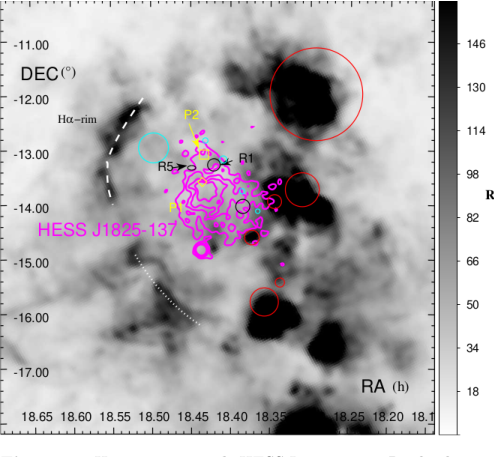
\includegraphics[width=0.5\textwidth]{06_Interstellar_Medium/Images/Theory/Fabien_Halpha.pdf}
	\caption{H$\alpha$ intensity towards \mbox{HESS\,J1825-137}. The dashed and dotted lines represent two H$\alpha$ rim-like features associated with the progenitor SNR of \mbox{HESS\,J1825-137}. Image courtesy of \citep{2016MNRAS.458.2813V}}
	\label{fig:06_1825_SNR}
\end{SCfigure}

%\begin{wrapfigure}[30]{R}{0.45\textwidth}
%    \centering
%    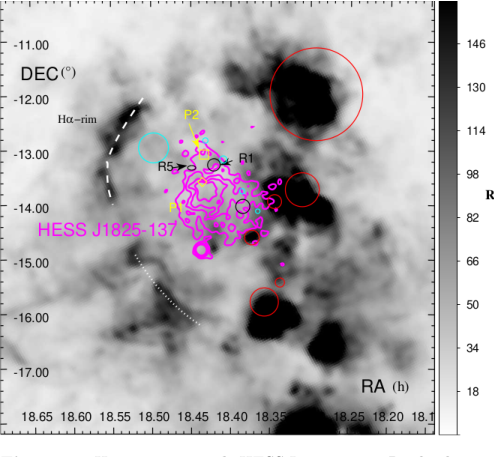
\includegraphics[width=0.45\textwidth]{06_Interstellar_Medium/Images/Theory/Fabien_Halpha.pdf}
%    \caption{H$\alpha$ intensity towards \mbox{HESS\,J1825-137}. The dashed and dotted lines represent two H$\alpha$ rim-like features associated with the progenitor SNR of \mbox{HESS\,J1825-137}. Image courtesy of \citep{2016MNRAS.458.2813V}}
%    \label{fig:06_1825_SNR}
%\end{wrapfigure}

Atomic hydrogen in clouds can be ionised by UV light from background stars to form HII regions, while shocks (SNRs), X-rays and cosmic rays leads to the ionisation of molecular hydrogen \citep{2011piim.book.....D}. Recombination of HII atoms and electrons may result in the the emission of light in the H$\alpha$ band (corresponding to a decay from the third to the second energy level). Hence H$\alpha$ emission can be used as a tracer for ionised hydrogen gas (HII gas). Shocks associated with SNRs ionise hydrogen gas, leading to H$\alpha$ rim-like features like those towards \mbox{HESS\,J1825-137} (see \autoref{fig:06_1825_SNR}). Both structures are located $\approx 120~\pc$ from \mbox{PSR\,J1826-1334} which is consistent with the predicted SNR radius ($\approx 130~\pc$) as suggested by \cite{deJager2009}.
\par~\par
Ionised gas towards \mbox{HESS\,J1825-137} acts as a target for cosmic rays escaping from the PWN/SNR to undergo hadronic/leptonic interactions and emit gamma radiation. The following describes two different methods to trace the ionised hydrogen within molecular clouds.

\subsubsection{Method A}

For a spherical shell of gas located at distance $d$ from the Earth with thickness $\dd{\ell}$, the volume of the shell is given by:
\begin{equation}
    \begin{aligned}
        \dd{V}&=2\pi d^2 \dd{\ell}\text{ ,}
    \end{aligned}
\end{equation}
\noindent where photons emitted by the gas travel at the speed of light, hence $\dd{\ell}=c\dd{t}$. The total number of photons emitted in the shell in time $\dd{t}$ is related to the luminosity, $L$, via:

\begin{equation}
    \begin{aligned}
        \dd{N}&=L\dd{t}\text{ ,}
    \end{aligned}
\end{equation}
\noindent where the luminosity of the region of interest with solid angle $\omega$ is:
\begin{equation}
    \begin{aligned}
        L\quad \qty[\text{photon/s}]&=\frac{d^2}{10^{-10}}\Omega I\text{ ,}
    \end{aligned}
\end{equation}
\noindent with $I$ being the measured H$\alpha$ in Rayleigh units ($=10^{10}~\si{ph\per\meter\squared\per\second\per{column}}$). Assuming atoms are not re-excited by an external source, the density of photons emitted by ionised gas $u_\text{ph}$ is approximately equal to the ionised gas density $n_\text{ion}$:

\begin{equation}
    \begin{aligned}
        n_\text{ion}\approx u_\text{ph}=\dv{N}{V}=\frac{L}{4\pi d^2 c}\text{ .}
    \end{aligned}
\end{equation}

\subsubsection*{Method B}

For photons of frequency $\nu$, the photon intensity ($I_\nu$) is related to the luminosity ($L$) through:

\begin{equation}
    \begin{aligned}
        I_\nu=L\frac{E_\nu}{\nu}=hL\text{ ,}
    \end{aligned}
\end{equation}
\noindent where $h$ is Planck's constant. For a cloud with thickness $s$, the emission coefficient is given by:

\begin{equation}
    \begin{aligned}
        j_\nu&=\frac{I_\nu}{s}\text{ ,}
    \end{aligned}
\end{equation}
\noindent assuming that the emission coefficient is constant throughout the gas. Hence, the density of atoms in the ith state emitting photons at frequency $\nu$ via spontaneous emission:

\begin{equation}
	\begin{aligned}
		n_i&=\frac{j_\nu \Omega_\text{Earth}}{E_\nu A\phi (\nu)}\text{ ,}
	\end{aligned}\label{eq:interstellar_medium_halpha_dens_2}
\end{equation}
where A is the Einstein coefficient, $\Omega_\text{earth}$ is the solid angle of Earth projected at source lying at distance $d$ and $\phi(\nu)$ is the spectral line shape normalised by:
\begin{equation}
	\begin{aligned}
		\int \phi(\nu)=1\text{ .}
	\end{aligned}
\end{equation}
Assuming that hydrogen atoms in the $n=3$ state emit mainly H$\alpha$ light; $\phi=0$ in all frequencies except when $\nu=\nu_{H\alpha}$. 

\subsection{Nanten2 Observatory} \label{sec:NANTEN}

\begin{figure} [h]
    \centering
    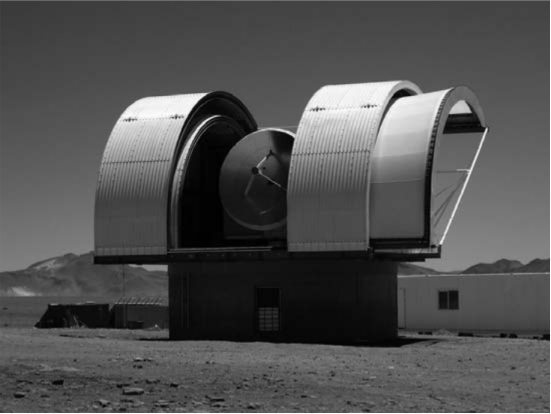
\includegraphics[width=0.7\textwidth]{06_Interstellar_Medium/Images/Observatories/Nanten2.pdf}
    \caption{Nanten2 telescope. Image courtesy of \cite{2006IAUSS...1E..21F}.}
    \label{fig:interstellar_medium_NANTEN}
\end{figure}

Nanten2 (Japanese for `Southern Sky') is an upgrade to the $4\m$ Nanten telescope originally located in Las Campanas before its relocation to the Atacama desert in Chile in 2004 \citep{2006IAUSS...1E..21F}. Nanten2 is located at altitude $4800~\m$ and consists of 33 adjustable aluminum panels on a light-weight carbon fiber back structure. Nanten2 is sensitive to atomic and molecular spectral lines  $100-880~\si{\hertz}$ and has angular resolution up to $2'6$ beam size \citep{2001PASJ...53L..45M}, allowing detailed observations of gas structures. Nanten2 has conducted multiple CO surveys of regions such as the Large Magnetic Cloud \citep{Kawamura_2009} and the Galactic plane \citep{2004ASPC..317...59M} covering velocity range $-300~\kmpersec$ to $300~\kmpersec$ with a velocity resolution up to $1.0~\kmpersec$.
\par~\par
\cite{2016MNRAS.458.2813V} conducted an ISM gas study towards PWN \mbox{HESS\,J1825-137} and \mbox{HESS\,J1826-130} utilising Nanten2 data. They found that the majority of gas towards this region is located in the velocity range $45-60~\kmpersec$ ($3.8-4.5~\kpc$) which is equivalent to the dispersion measure distance of the associated pulsar \mbox{PSR\,J1826-134}. \cite{2016MNRAS.458.2813V} noted six clouds of interest, named R1-R6, whose parameters are summarised in \autoref{tab:06_fabien_cloud_summary}. Cloud R1 was noted to show enhanced turbulence possibly due to the associated SNR shock or the formation of high-mass stars.
\begin{table}[h!]
    \caption{Derived parameters for clouds R1-R6 towards \mbox{HESS\,J1825-137} and \mbox{HESS\,J1826-130} utilising Nanten2 CO(J=1-0) from \cite{2016MNRAS.458.2813V}}
    \begin{threeparttable}
    \centering
    \begin{tabular}{cccccc}
        \toprule
        Cloud & RA ($\si{h}$) & DEC ($\si{\degree}$)& Radii ($''$) & $n_H$ ($\centimeterminusthree$) & $M_H$ ($M_\odot$) \\
        \midrule
        R1 & $18.421$ & $-13.282$ & $405\times 405$ & $960$ & $1.2\times 10^5$ \\
        R2 & $18.420$ & $-13.125$ & $135\times 270$ & $1200$ & $1.3\times 10^4$ \\
        R3 & $18.429$ & $-13.178$ & $64\times 64$ & $1600$ & $3.3\times 10^3$ \\
        R4 & $18.422$ & $-12.832$ & $175\times 280$ & $930$ & $1.6\times 10^4$ \\
        R5 & $18.449$ & $-13.336$ & $150\times 270$ & $680$ & $9.5\times 10^3$  \\
        R6 & $18.385$ & $-14.049$ & $460\times 460$ & $430$  & $7.6\times 10^4$ \\
        \bottomrule
    \end{tabular}
 %    \begin{tablenotes}
	% \item \textbf{References}
	% \item a: \citep{2020A&A...644A.112H}
 %    \end{tablenotes}
    \end{threeparttable}
    \label{tab:06_fabien_cloud_summary}
\end{table}
\chapter[Time evolution of CR particles]{Time evolution of cosmic ray particles from an accelerator} \label{sec:07_particle_ev}

Cosmic Rays (electrons and protons) are accelerated by sources such as PWNe and SNRs. Cosmic rays then escape the acceleration regions and subsequently propagate through the interstellar medium, losing energy through various processes such as radiative cooling, adiabatic expansion and ionisation as discussed in \autoref{sec:chapter1_non_thermal_emission}. By modelling the transport of cosmic-ray particles from an accelerator, the subsequent gamma-ray distribution can be predicted (see \autoref{sec:chapter1_non_thermal_emission}) and compared to observations.
\par~\par
This section first discusses how the energy distribution of cosmic rays evolves in time due to radiation losses and predicts the subsequent gamma-ray emission. This will then be expanded to include the escape of cosmic rays out of the region of interest due to diffusion (see \autoref{chapter_1_cr_propagation}). Finally, this section describes the numerical code developed by \cite{fabien}, which can be used for systems where the cosmic-ray energy distribution and the gamma-ray SED cannot be solved analytically.
\par~\par
This code was applied to investigate the origin of the $\GeV$ gamma-ray emission to the south of \mbox{HESS\,J1825-137}. Proposed sources included the impulsive SNR and continuous PWN associated with \mbox{HESS\,J1825-137} and the impulsive SNR and continuous compact object binary associated with \mbox{LS\,5039}. The results of this study were published in the Monthly Notices of the Royal Astronomical Society and is shown in \autoref{sec:08}.

\section{Radiation Losses} \label{sec:chapter_7_cr_SED_evol} 

First consider cosmic rays being injected by a homogeneous source into a region of interest at rate $S\qty(\gamma,t)$ and escaping at rate $v_\text{esc}$. The time evolution of the cosmic-ray energy density distribution, $n\qty(\gamma,t)$, can be described by \citep{1980gbs..bookR....M}:
%The time evolution of the cosmic ray energy distribution, $n\qty(\gamma,t)$ for a homogeneous source injecting particles at rate $S\qty(\gamma,t)$ and escape rate $v_\text{esc}$ can be described by \citep{1980gbs..bookR....M}:

\begin{equation}
    \begin{aligned}
    \pdv{n\qty(\gamma,t)}{t}&=\pdv{ }{\gamma}\qty[\dot{\gamma}\qty(\gamma)n\qty(\gamma, t)] - \nu_\text{esc}\qty(\gamma)n\qty(\gamma,t) + S\qty(\gamma, t)\text{ ,}
    \end{aligned} \label{eq:chapter_7_cr_energy_distribution}
\end{equation}
\noindent where cosmic rays with Lorentz Factor $\gamma$ continuously lose energy at rate $\dv{\gamma}{t}=\dot{\gamma}$ and have probability $v_\text{esc}\dd{t}$ of escaping the system in time $\dd{t}$. Physically, $\dot{\gamma}\qty(\gamma)n\qty(\gamma,t)$ is the number of cosmic rays per unit time that cool at Lorentz factor $\gamma$ for a cosmic-ray density $n$. The following will describe the solution of \autoref{eq:chapter_7_cr_energy_distribution} using Laplace transformations.
\par~\par
Laplace transformations are used to reduce differential equations conveniently into an algebraic equation. The Laplace Transform for the function $f\qty(t)$ is given by:

\begin{equation}
    \begin{aligned}
        \bar{f}\qty(q)&=\int_0^\infty e^{-qt}f\qty(t)\dd{t}\text{ .}
    \end{aligned}
\end{equation}
\noindent Similarly, the Laplace transformation for $f'\qty(t)=\dv{f}{t}$:

\begin{equation}
	\begin{aligned}
		\bar{f}'\qty(q)&=q\bar{f}\qty(q)-f\qty(0)\text{ .}
	\end{aligned}
\end{equation}
\noindent Hence, the Laplace transformation of \autoref{eq:chapter_7_cr_energy_distribution}:

\begin{equation}
    \begin{aligned}
        q\bar{n}\qty(\gamma, q)-n\qty(\gamma,0)&=\pdv{}{\gamma}\qty[\dot{\gamma}\qty(\gamma)\bar{n}\qty(\gamma, q)] - \nu_\text{esc}\qty(\gamma)\bar{n}\qty(\gamma,q) + \bar{S}\qty(\gamma, q) \\
        -\bar{S}\qty(\gamma,q)-n\qty(\gamma,0)&=\pdv{}{\gamma}\qty[\dot{\gamma}\bar{n}\qty(\gamma,q)]-\qty[q+\nu_\text{esc}\qty(\gamma)]\bar{n}\qty(\gamma,q)\text{ .}
    \end{aligned} \label{eq:chapter_7_cr_energy_distribution_transform}
\end{equation}
\noindent The variable $Q\qty(\gamma,q)=\dot{\gamma}\bar{n}\qty(\gamma,q)$ is defined such that \autoref{eq:chapter_7_cr_energy_distribution_transform} becomes:

\begin{equation}
    \begin{aligned}
        -\bar{S}\qty(\gamma,q)-n\qty(\gamma,0)&=\pdv{}{\gamma}Q\qty(\gamma,q)-\qty[q+\nu_\text{esc}\qty(\gamma)]\frac{Q\qty(\gamma,q)}{\dot{\gamma}}\text{ ,}
    \end{aligned}  \label{eq:chapter_7_cr_energy_distribution_transform2}
\end{equation}
\noindent $Q\qty(\gamma,q)$ can be described as the number of cosmic rays per unit time that cool from Lorentz factor $\gamma$. The differential equation describing the time evolution of the cosmic-ray energy density distribution has been reduced to a first order linear differential equation of form:

\begin{equation}
	\begin{aligned}
		b\qty(x)&=\dv{y}{x}+a\qty(x)y\text{ ,}
	\end{aligned}
\end{equation}

\noindent which has solution:

\begin{equation}
    \begin{aligned}
        y\qty(x)&=e^{-A\qty(x)}\int_{x'=x} e^{A\qty(x')}b\qty(x')\dd{x'}\text{ ,}
    \end{aligned}
\end{equation}

\noindent where $A\qty(x)=\int_{x''=x} a\qty(x'') \dd{x''}$. Therefore, the solution of \autoref{eq:chapter_7_cr_energy_distribution_transform2} is given by:

\begin{equation}
	\begin{aligned}
		Q\qty(\gamma,q)&=e^{\int_{\gamma''=\gamma}\dd{\gamma''}\qty[q+\nu_\text{esc}]/\dot{\gamma}}\int_{\gamma'=\gamma} e^{-\int_{\gamma''=\gamma'}\dd{\gamma''}\qty[q+\nu_\text{esc}]/\dot{\gamma}}\qty[\bar{S}\qty(\gamma',q)+n\qty(\gamma',0)]\dd{\gamma'}\text{ .}
	\end{aligned} \label{eq:07_solution_Q}
\end{equation}
\noindent Following \cite{1980gbs..bookR....M}, the time required for a cosmic ray to cool from Lorentz factor $\gamma'$ to $\gamma$ is given by:

\begin{equation}
    \begin{aligned}
    \tau\qty(\gamma', \gamma) &= \int_{\gamma''=\gamma'} \dd{\gamma''}\frac{1}{\dot{\gamma}\qty(\gamma'')} - \int_{\gamma''=\gamma} \dd{\gamma''}\frac{1}{\dot{\gamma}\qty(\gamma'')}\\
    &=\int_\gamma^{\gamma'}\dd{\gamma''}\frac{1}{\dot{\gamma}\qty(\gamma'')}\text{ ,}
    \end{aligned} \label{eq:chapter_7_cooling_time}
\end{equation}
\noindent where $\gamma_0$ is the original Lorentz factor (at $t=0$) of a cosmic ray before cooling to Lorentz factor $\gamma$, i.e. $\tau(\gamma_0,\gamma)=t$. The term $\lambda\qty(\gamma',\gamma)$ is defined such that $1-\exp[-\lambda\qty(\gamma',\gamma)]$ is the probability that the cosmic ray escapes the region of interest while cooling from Lorentz factor $\gamma'$ to $\gamma$:

\begin{equation}
    \begin{aligned}
    \lambda\qty(\gamma',\gamma)&=\int_{\gamma''=\gamma'}\dd{\gamma''}\frac{\nu_\text{esc}\qty(\gamma'')}{\dot{\gamma}\qty(\gamma'')}-\int_{\gamma''=\gamma}\dd{\gamma''}\frac{\nu_\text{esc}\qty(\gamma'')}{\dot{\gamma}\qty(\gamma'')} \\
    &=\int_\gamma^{\gamma'}\dd{\gamma''}\frac{\nu_\text{esc}\qty(\gamma'')}{\dot{\gamma}\qty(\gamma'')}\text{ .}
    \end{aligned} \label{eq:chapter_7_lambda_escape_rate}
\end{equation}
\noindent Therefore, \autoref{eq:07_solution_Q} has solution:

\begin{equation}
    \begin{aligned}
        Q\qty(\gamma,q)&=\int_\gamma^\infty e^{-\qty[q\tau\qty(\gamma',\gamma)+\lambda\qty(\gamma',\gamma)]}\qty{\bar{S}\qty(\gamma',q)+n\qty(\gamma',0)}\dd{\gamma'} \\
        \bar{n}\qty(\gamma,q) &=\frac{1}{\dot{\gamma}}\int_\gamma^\infty e^{-\lambda\qty(\gamma',\gamma)} \qty{e^{-q\tau\qty(\gamma',\gamma)}\bar{S}\qty(\gamma',s)+e^{-q\tau\qty(\gamma',\gamma)}n\qty(\gamma',0)}\dd{\gamma'}\text{ .}
    \end{aligned} \label{eq:chapter_7_cr_energy_distribution_transform_sol}
\end{equation}
\noindent The following inverse Laplace transformations can be used to obtain the cosmic-ray energy density distribution $n\qty(\gamma,t)$ from \autoref{eq:chapter_7_cr_energy_distribution_transform_sol}:

\begin{equation}
    \begin{alignedat}{2}
    e^{-cq}\bar{f}\qty(q) &\longleftrightarrow && H\qty(t-c)f\qty(t) \\
    e^{-cq} &\longleftrightarrow && \delta\qty(t-c)\text{ ,}
\end{alignedat}
\end{equation}
\noindent with $H$ is the Heaviside step function and $\delta$ is the Dirac delta function. Therefore, \autoref{eq:chapter_7_cr_energy_distribution} has solution:

\begin{equation}
    \begin{aligned}
        n\qty(\gamma,t)&=\frac{1}{\dot{\gamma}}\int_\gamma^\infty e^{-\lambda\qty(\gamma',\gamma)} \qty{H\qty(t-\tau\qty(\gamma',\gamma))S\qty(\gamma',t-\tau\qty(\gamma',\gamma))+\delta\qty(t-\tau\qty(\gamma',\gamma))n\qty(\gamma',0)}\dd{\gamma'}  \\
        &=\frac{1}{\dot{\gamma}}\int_\gamma^{\gamma_0}  e^{-\lambda\qty(\gamma',\gamma)} S\qty(\gamma',t-\tau\qty(\gamma',\gamma))\dd{\gamma'}  + \frac{\dot{\gamma}_0}{\dot{\gamma}}e^{-\lambda\qty(\gamma_0,\gamma)} n\qty(\gamma_0,0)\text{ ,}
    \end{aligned}  \label{eq:chapter_7_cr_energy_distribution_sol}
\end{equation}
\noindent where $\gamma_0$ is the original Lorentz factor (at $t=0$) of a cosmic ray before cooling to Lorentz factor $\gamma$, i.e. $\tau\qty(\gamma_0,\gamma)=t$. \autoref{eq:chapter_7_cr_energy_distribution_sol} describes the cosmic-ray energy density distribution at time $t$ with Lorentz factor $\gamma$. In order to solve \autoref{eq:chapter_7_cr_energy_distribution_sol} analytically, impulsive and continuous accelerator sources will be treated separately. 

\subsection{Impulsive Source of Cosmic Rays}

An impulsive source is a source of cosmic rays (and/or electrons) that injects material into the ISM at one point in time instantaneously or over a time period much less than the observation time. Examples of impulsive sources include supernovae, SNRs or gamma-ray bursts. The source term of an impulsive source can be described by $S\qty(\gamma,t>0)=0$. Assuming that cosmic rays do not escape the system ($\lambda=0$), \autoref{eq:chapter_7_cr_energy_distribution_sol} becomes:

\begin{equation}
    \begin{aligned}
    n\qty(\gamma,t)&=\frac{\dot{\gamma_0}}{\dot{\gamma}}n\qty(\gamma_0,0)\exp(-\lambda\qty(\gamma_0,\gamma))\text{ .}
    \end{aligned} \label{eq:chapter_7_cr_energy_distribution_imp} 
\end{equation}

The cosmic-ray flux at Earth tends to follow a power law spectrum (see \autoref{sec:chapter_1_cr_spectrum}), suggesting that sources inject cosmic rays with a power law energy distribution. Hence, it will be assumed that injected particles can be described by an exponential cutoff power law spectrum:

\begin{equation}
    \begin{aligned}
    n\qty(\gamma_0,0)&=\tilde{A}E^{-\Gamma}\exp(-\frac{E}{E_c})=\tilde{A}\qty(\gamma_0 mc^2)^{-\Gamma}\exp(-\frac{\gamma_0 mc^2}{\gamma_c mc^2}) \\
	&=A\gamma_0^{-\Gamma}\exp(-\frac{\gamma_0}{\gamma_c})\text{ ,}
    \end{aligned} \label{eq:chapter_7_cr_energy_distribution_imp_t0} 
\end{equation}
\noindent where $\Gamma$ is the spectral index, $A=\tilde{A}\qty(mc^2)^{-\Gamma}$ is the normalisation factor and $E_c$ and $\gamma_c$ are the cutoff energy and cutoff Lorentz factor respectively.

\subsubsection{Hadronic Cosmic-Ray Source}

Hadronic cosmic rays lose their energies through proton-proton interactions with the ISM (see \autoref{sec:chapter1_hadronic_gr_emission}). The energy loss rate of hadronic cosmic rays with Lorentz factor $\gamma$ is approximated by \cite{1996A&A...309..917A}:

\begin{equation}
    \begin{aligned}
    \dot{\gamma}&=-\frac{\gamma}{\tau_{pp}} \text{ ,}
    \end{aligned} \label{eq:chaper_7_hadron_loss_rate}
\end{equation}
\noindent where $\tau_{pp}$ is the p-p cooling time (\autoref{eq:chapter_1_pp_cooling time}). The cooling time is inversely proportional to the p-p cross section, $\sigma_{pp}$, where the p-p cross section is weakly dependent on the proton energy (see \autoref{eq:chapter1_non_thermal_pp_cross_section}). The solution to \autoref{eq:chaper_7_hadron_loss_rate} is:

\begin{equation}
    \begin{aligned}
        \gamma&=\gamma_0\exp(-t/\tau_{pp})\text{ .}
    \end{aligned} \label{eq:chapter_7_hadron_loss_solution}
\end{equation}
\noindent The initial cosmic-ray energy distribution can be rewritten in terms of $\gamma$:

\begin{equation}
    \begin{aligned}
    	n_p\qty(\gamma_0,0)&=A\gamma^{-\Gamma} \exp(-\frac{\Gamma t}{\tau_{pp}})\exp(\frac{-\gamma\exp(t/\tau_{pp})}{\gamma_c}) \text{ .}
    \end{aligned} \label{eq:chapter_7_imp_hadronic_cr_initial_distrib}
\end{equation}
\noindent As $\dot{\gamma}_0=-\gamma_0/\tau_{pp}$:

\begin{equation}
	\begin{aligned}
		\frac{\dot{\gamma}_0}{\dot{\gamma}}=\frac{\gamma_0}{\gamma}=\exp(t/\tau_{pp})\text{ .}
	\end{aligned} \label{eq:07_hadron_gammadot_ratio}
\end{equation}

\autoref{eq:chapter_7_cr_energy_distribution_imp} and \autoref{eq:chapter_7_imp_hadronic_cr_initial_distrib} can be combined to find the energy density distribution of cosmic rays for an impulsive source injecting protons with an exponential cutoff power law spectrum:

\begin{equation}
    \begin{aligned}
       	n_p\qty(\gamma,t)&=A\gamma^{-\Gamma}\exp(-\frac{\qty(\Gamma-1)t}{\tau_{pp}}-\frac{\gamma\exp(t/\tau_{pp})}{\gamma_c})\text{ .}
    \end{aligned} \label{eq:chapter_7_imp_hadronic_cr_energy_distrib}
\end{equation}
\begin{figure}[hbtp]
	\centering
	\includegraphics[width=1.0\textwidth]{07_Particle_Evolution/Images/evolution/impulsive_proton_total_spectrum.pdf}
	\caption{Evolution of the cosmic-ray energy density distribution (\textit{top}) and subsequent gamma-ray SED (\textit{bottom}) for an impulsive source injecting protons following a power law spectrum ($\propto E^{-\Gamma}$, red) and an exponential cutoff power law spectrum ($\propto E^{-\Gamma}\exp(-E/E_c)$, black) as given by \autoref{eq:chapter_7_imp_hadronic_cr_energy_distrib}. $W_p$ is the total energy of cosmic-ray protons injected at $t=0$.1q}
	\label{fig:chapter_7_impulsive_hadron_cr_spectrum}
\end{figure}

The top panel of \autoref{fig:chapter_7_impulsive_hadron_cr_spectrum} shows the evolution of a hadronic cosmic-ray energy density distribution and subsequent gamma-ray SED for an initial power law spectrum ($\Gamma=2.2$) and an exponential cutoff power law spectrum ($\Gamma=2.2$, $E_c=100~\TeV$). As the age of the system increases beyond the proton cooling time (i.e. $t>\tau_{pp}=5.3\times 10^5~\si{yr}$), the cosmic-ray density and subsequent gamma-ray emission decreases (see \autoref{sec:chapter1_hadronic_gr_emission}).

\subsubsection{Leptonic Cosmic-Ray Source}

Assuming synchrotron losses are dominant (valid for high-energy electrons and/or regions of high magnetic field strength, see \autoref{eq:chapter_1_non_thermal_leptonic_cooling_rate2}), the leptonic cooling rate is given by:

\begin{equation}
    \begin{aligned}
        \dot{\gamma}&=-b_s\gamma^2 \text{ ,}
    \end{aligned}\label{eq:chapter_7_lepton_loss_rate}
\end{equation}
\noindent where $b_s = 1.292 \times 10^{-15} \qty(B/\si{\milli G})^2~\si{\per\second}$ is the synchrotron loss term for electrons. The solution for \autoref{eq:chapter_7_lepton_loss_rate} is:

\begin{equation}
	\begin{aligned}
		\gamma_0&=\frac{\gamma}{1-\gamma b_s t} \text{ ,}
	\end{aligned} \label{eq:chapter_7_imp_leptonic_lorentz_initial}
\end{equation}
\noindent giving the initial electron distribution in terms of Lorentz factor $\gamma$:
\begin{equation}
    \begin{aligned}
        n_e\qty(\gamma_0,0)&=A\gamma^{-\Gamma}\qty(1-\gamma b_s t)^{\Gamma}\exp(-\frac{\gamma}{\gamma_c\qty(1-\gamma b_st)})\text{ .} 
    \end{aligned} \label{eq:chapter_7_imp_leptonic_cr_initial_distrib}
\end{equation}
\noindent From \autoref{eq:chapter_7_imp_leptonic_lorentz_initial} it can be seen that at any time, $t$, there exists a critical Lorentz factor:

\begin{equation}
    \begin{aligned}
    \gamma_\text{cr}&=\frac{1}{b_s t} \text{ ,}
    \end{aligned}\label{eq:chapter_7_imp_lep_critical_lorentz}
\end{equation}
\noindent where electrons with $\gamma_\text{cr}$ have an initial Lorentz factor, $\gamma_0\rightarrow \infty$. An impulsive system at time $t$ cannot have electrons exceeding this critical Lorentz factor.
\par
\noindent As $\dot{\gamma}_0=-b_s\gamma^2$:

\begin{equation}
	\begin{aligned}
		\frac{\dot{\gamma}_0}{\dot{\gamma}}&=\qty(\frac{\gamma_0}{\gamma})^2 \text{ ,}
	\end{aligned} \label{eq:chapter_7_gamma_gamma_0_ratio}
\end{equation}
\noindent \autoref{eq:chapter_7_cr_energy_distribution_imp} and \autoref{eq:chapter_7_imp_leptonic_cr_initial_distrib} can be combined to find the cosmic-ray energy density distribution for electrons with Lorentz factor $\gamma$:

\begin{equation}
    \begin{aligned}
    n_e\qty(\gamma,t)&=A\gamma^{-\Gamma}\qty(1-\gamma b_s t)^{\Gamma-2}\exp(-\frac{\gamma}{\gamma_c\qty(1-\gamma b_st)})\text{ .}
    \end{aligned} \label{eq:chapter_7_imp_leptonic_cr_energy_distrib}
\end{equation}
\begin{figure}[hbtp]
	\centering
	\includegraphics[width=1.0\textwidth]{07_Particle_Evolution/Images/evolution/impulsive_electron_total_spectrum.pdf}
	\caption{Evolution of the cosmic-ray energy density distribution (\textit{top}) and subsequent gamma-ray SED (\textit{bottom}) for an impulsive source injecting electrons following a power law spectrum (red) and an exponential cutoff power law spectrum (black) as given by \autoref{eq:chapter_7_imp_leptonic_cr_energy_distrib}. The critical Lorentz factor (\autoref{eq:chapter_7_imp_lep_critical_lorentz}) at different ages are shown by the vertical blue-dashed lines.}
	\label{fig:chapter_7_impulsive_lepton_cr_spectrum}
\end{figure}
\autoref{fig:chapter_7_impulsive_lepton_cr_spectrum} shows the energy density distribution evolution of electrons and the subsequent gamma-ray emission for an impulsive source with an initial power law and exponential cutoff power law spectrum. As the system ages, the critical Lorentz factor (see \autoref{eq:chapter_7_imp_lep_critical_lorentz}) decreases and the energy density distribution can be described by an exponential cutoff power regardless of the distribution at times, $t=0~\si{\year}$. The peak in the subsequent synchrotron and inverse Compton emission shifts to lower energies as the system evolves in time.


\subsection{Continuous Source of Cosmic Rays}

A continuous source is a source that injects cosmic rays into the ISM at a constant rate over a significant time frame. For simplicity, it's assumed that source has a constant injection luminosity; i.e. no outbursts or `dormant' stages. Examples of continuous sources include pulsars and massive stellar clusters which typically inject cosmic rays for over $10^5~\si{yr}$. At $t=0~\si{yr}$ the initial cosmic-ray density, $n\qty(\gamma_0,0)$, is zero. Assuming that no cosmic rays escape the system ($\lambda=0$), \autoref{eq:chapter_7_cr_energy_distribution_transform_sol} becomes:

\begin{equation}
    \begin{aligned}
    	n\qty(\gamma,t)&=\frac{1}{\dot{\gamma}\qty(\gamma)}\int_\gamma^{\gamma_0} S\qty(\gamma',t-\tau\qty(\gamma',\gamma))\dd{\gamma'} \text{ ,}
    \end{aligned} \label{eq:chapter_7_cr_energy_distribution_cont} 
\end{equation}
\noindent and it will be assumed that the electron energy distribution of accelerators such as PWNe follow a power law (e.g. \citep{2014JHEAp...1...31T}). Hence, the source term in \autoref{eq:chapter_7_cr_energy_distribution_cont} will follow:

\begin{equation}
    \begin{aligned}
    S\qty(\gamma,t)&=A\gamma^{-\Gamma} \text{ .}
    \end{aligned} \label{eq:chapter_7_cr_energy_distribution_cont_t0} 
\end{equation}

\subsubsection{Hadronic Cosmic-Ray Source}

Combining \autoref{eq:chaper_7_hadron_loss_rate}, \autoref{eq:chapter_7_hadron_loss_solution}, \autoref{eq:chapter_7_cr_energy_distribution_cont} \& \autoref{eq:chapter_7_cr_energy_distribution_cont_t0} gives the proton energy density distribution at Lorentz factor $\gamma$:

\begin{equation}
    \begin{aligned}
    n_p\qty(\gamma,t)&=\frac{A\tau_{pp}}{\gamma}\int_\gamma^{\gamma_0} \gamma^{-\Gamma} \dd{\gamma'} \\
	&=\frac{A\tau_{pp}}{\gamma(\Gamma-1)}\qty[\gamma^{1-\Gamma}-\gamma_0^{1-\Gamma}] \\
	&=\frac{A\tau_{pp}}{\gamma(\Gamma-1)}\qty[\gamma^{1-\Gamma}-\qty(\gamma\exp(t/\tau_{pp}))^{1-\Gamma}] \\
	&=\frac{A\tau_{pp}\gamma^{\Gamma}-1}{\gamma(\Gamma-1)}\qty[1-\exp(-\frac{t\qty(\Gamma-1)}{\tau_{pp}})] \\
	&=\frac{\tau_{pp}A\gamma^{-\Gamma}}{\Gamma-1}\qty[1-\exp(-\frac{t\qty(\Gamma-1)}{\tau_{pp}})] \text{ .}
    \end{aligned} \label{eq:chapter_7_cont_hadronic_cr_energy_distrib}
\end{equation}

At $t=0$, the cosmic-ray energy density distribution is initially zero. As the system ages ($t\gg\tau_{pp}$), a steady state occurs when the energy loss through p-p interactions is balanced by the energy injected by the source (see \autoref{fig:chapter_7_continuous_hadron_cr_spectrum}). The steady state ($t\gg \tau_{pp}$) has an energy spectrum:
\begin{equation}
    \begin{aligned}
    	n_p\qty(\gamma, t\gg \tau_{pp})&=\frac{\tau_{pp}A\gamma^{-\Gamma}}{1-\Gamma}\text{ .}
    \end{aligned} \label{eq:07_cont_hadronic_cr_steady_state}
\end{equation}
\begin{figure}[hbtp]
	\centering
	\includegraphics[width=1.0\textwidth]{07_Particle_Evolution/Images/evolution/continuous_proton_total_spectrum.pdf}
	\caption{Evolution of the cosmic-ray energy density distribution (top) and subsequent gamma-ray spectrum (bottom) for a continuous source injecting protons following a power law spectrum as given by \autoref{eq:chapter_7_cont_hadronic_cr_energy_distrib}. The steady state ($t\gg \tau_{pp}$, see \autoref{eq:07_cont_hadronic_cr_steady_state}) is represented by the solid red line. $L_p$ is the energy of cosmic rays injected per second into the system.}
	\label{fig:chapter_7_continuous_hadron_cr_spectrum}
\end{figure}
\autoref{fig:chapter_7_continuous_hadron_cr_spectrum} shows the evolution of the cosmic-ray and subsequent gamma-ray spectra for a system that continuously injects protons into a system with proton-proton cooling time of $5.7\times 10^5~\si{yr}$.

\subsubsection{Leptonic Cosmic-Ray Source}
Again, synchrotron radiation is assumed to be the dominant cause of electron energy loss. From \autoref{eq:chapter_7_imp_leptonic_lorentz_initial} \& \autoref{eq:chapter_7_imp_lep_critical_lorentz}, electrons with Lorentz factor greater than the critical Lorentz factor ($\gamma\geq\gamma_\text{cr}$) must be treated separately:

\begin{equation}
    \begin{aligned}
    	n_e\qty(\gamma)&=
	\begin{cases}
	\frac{1}{\dot{\gamma}\qty(\gamma)}\int_{\gamma}^{\gamma_0}S\qty(\gamma',t-\tau\qty(\gamma',\gamma))\dd{\gamma'}  &\gamma < \gamma_\text{cr}\\
	\frac{1}{\dot{\gamma}\qty(\gamma)}\int_{\gamma}^{\infty}S\qty(\gamma',t-\tau\qty(\gamma',\gamma))\dd{\gamma'} &\gamma \geq \gamma_\text{cr}\\
	\end{cases}\text{ .} \label{eq:chapter_7_cr_energy_dist_lept_cont_final}
    \end{aligned}
\end{equation}
\noindent For $\gamma < \gamma_\text{cr}$, combining \autoref{eq:chapter_7_lepton_loss_rate}, \autoref{eq:chapter_7_imp_leptonic_lorentz_initial}, \autoref{eq:chapter_7_cr_energy_distribution_cont_t0} \& \autoref{eq:chapter_7_cr_energy_dist_lept_cont_final}:

\begin{equation}
    \begin{aligned}
    	n_e\qty(\gamma< \gamma_\text{cr})&=\frac{A}{b_s\gamma^2\qty(\Gamma-1)}\qty[\gamma^{1-\Gamma}-\gamma_0^{1-\Gamma}] \\
	&=\frac{A}{b_s\gamma^2\qty(\Gamma-1)}\qty[\gamma^{1-\Gamma}-\frac{\gamma^{1-\Gamma}}{\qty(1-\gamma b_s t)^{1-\Gamma}}] \\
	&=\frac{A\gamma^{-\Gamma}\gamma}{b_s\gamma^2\qty(\Gamma-1)}\qty[1-\frac{1}{\qty(1-\gamma b_s t)^{1-\Gamma}}] \\
	&=\frac{A\gamma^{-\Gamma}}{b_s\gamma\qty(\Gamma-1)}\qty[1-\qty(1-\gamma b_s t)^{\Gamma-1}]\text{ .}
    \end{aligned}
\end{equation}
\noindent For $\gamma \geq \gamma_\text{cr}$:

\begin{equation}
    \begin{aligned}
    n_e\qty(\gamma\geq \gamma_\text{cr})&=\frac{A}{b_s\gamma^2\qty(1-\Gamma)}\qty(\infty^{1-\Gamma}-\gamma^{1-\Gamma}) \\
	&=\frac{A\gamma^{-\Gamma}}{b_s\gamma\qty(\Gamma-1)}\text{ .}
    \end{aligned}
\end{equation}
\noindent Therefore:

\begin{equation}
    \begin{aligned}
    n_e\qty(\gamma)&=\frac{A\gamma^{-\Gamma}}{b_s\gamma\qty(\Gamma-1)}
	\begin{cases}
		\qty[1-\qty(1-\gamma b_s t)^{\Gamma-1}] &\gamma < \gamma_\text{cr}\\
		1 &\gamma \geq \gamma_\text{cr}\\
	\end{cases} \text{ .}
    \end{aligned} \label{eq:chapter_7_cont_leptonic_cr_energy_distrib}
\end{equation}
\noindent A steady state is reached when:

\begin{equation}
    \begin{aligned}
        t\equiv\tau = (\gamma b_s)^{-1} = \tau_\text{sync}\text{ ,}
    \end{aligned} \label{eq:07_cont_leptonic_cr_steady_state}
\end{equation}
\begin{figure} [hbtp]
	\centering
	\includegraphics[width=1.0\textwidth]{07_Particle_Evolution/Images/evolution/continuous_electron_total_spectrum.pdf}
	\caption{Evolution of the cosmic-ray energy density distribution (\textit{top}) and subsequent gamma-ray SED (\textit{bottom}) for a continuous source injecting electrons following a power law spectrum as given by \autoref{eq:chapter_7_cont_leptonic_cr_energy_distrib}. The steady state of electrons ($t\gg \tau\approx \tau_\text{sync}$, see \autoref{eq:07_cont_leptonic_cr_steady_state}) is represented by the dash-dot line. $L_e$ is the energy of electrons injected per second into the system.}
	\label{fig:chapter_7_continuous_lepton_cr_spectrum}
\end{figure}

\noindent where $\tau_\text{sync}$ is the cooling time of electrons through synchrotron emission. The evolution of the electron spectra and subsequent gamma-ray spectra is shown in \autoref{fig:chapter_7_continuous_lepton_cr_spectrum}. Unlike protons, where the cooling time, $\tau_{pp}$, is dependent only on the medium's number density, the cooling time for electrons through synchrotron radiation is inversely proportional to their energy. Therefore, high-energy electrons reach a steady state before lower energy electrons.

\section{Transport of Cosmic Rays} \label{sec:chapter_7_cr_SED_trans} 

\autoref{eq:chapter_7_imp_hadronic_cr_energy_distrib}, \autoref{eq:chapter_7_imp_leptonic_cr_energy_distrib}, \autoref{eq:chapter_7_cont_hadronic_cr_energy_distrib} and \autoref{eq:chapter_7_cont_leptonic_cr_energy_distrib} describe the evolution of the spectral energy density distribution of cosmic rays at the location of the source. However, cosmic rays propagate from their place of birth into the ISM through diffusion (see \autoref{chapter_1_cr_propagation}). This section will describe how the cosmic-ray energy density distribution spatially and temporally evolves as a function of distance, $r$, from the accelerator.

\subsection{Propagation of Cosmic Rays}

We will take the simple example of an impulsive cosmic-ray source injecting particles with power law spectrum ($n\qty(\gamma,r=0,t=0)=A\gamma^{-\Gamma}$) into the centre of a uniform cloud at $t=0$. The cosmic rays are then allowed to propagate outwards. \cite{1995PhRvD..52.3265A} gives the Green's function solution of \autoref{eq:chapter_7_cr_energy_distribution_sol} at a distance $r$ from an impulsive source:

\begin{subequations}
	\begin{align}
	n\qty(\gamma,t,r)&=\frac{\dot{\gamma}_0}{\dot{\gamma}}\frac{n\qty(\gamma,0,0)}{\pi^{\frac{3}{2}}R_\text{diff}\qty(\gamma,t,B)^3}\exp\qty(-\frac{r^2}{R_\text{diff}\qty(\gamma,t,B)^2}) \label{eq:chapter_7_cr_ev_green_solution} \\
	R_\text{diff}\qty(\gamma,t,B)&=\sqrt{4\int_\gamma^{\gamma_0}\frac{D\qty(\gamma',B)}{\dot{\gamma}'}\dd{\gamma'}}\text{ ,} \label{eq:chapter_7_R_ev_green_solution}
	\end{align}
\end{subequations}  
\noindent where $R_\text{diff}\qty(\gamma,t)$ represents the distance of which cosmic rays with Lorentz factor $\gamma$ propagate after time $t$, i.e. `diffusion distance' and $D\qty(\gamma,B)$ represents the diffusion coefficient for cosmic rays in a magnetic field strength $B$ (see \autoref{eq:diffusion}).

\subsubsection{Hadronic Cosmic-Ray Source}

Combining \autoref{eq:chaper_7_hadron_loss_rate} and \autoref{eq:chapter_7_R_ev_green_solution} gives the evolution of the diffusion radius at distance $r$ from the accelerator:

\begin{equation}
	\begin{aligned}
		R_\text{diff}\qty(\gamma,t,B)&=\sqrt{4\tau_{pp}\chi D_0\qty(\frac{B}{3~\si{\micro G}})^{-\delta}\int_\gamma^{\gamma_0}\gamma'^{\delta-1}\dd{\gamma'}} \\
		&=\sqrt{4\tau_{pp}\chi D_0\qty(\frac{B}{3~\si{\micro G}})^{-\delta}\qty{\gamma_0^\delta-\gamma^\delta}} \\
		&=\sqrt{4\tau_{pp}\chi D_0\qty(\frac{B}{3~\si{\micro G}})^{-\delta}\qty{\gamma^\delta\exp\qty(\gamma t/\tau_{pp})-\gamma^\delta}} \\
		&=\sqrt{4D\qty(\gamma,B)t\frac{\qty(\exp(\frac{\delta t}{\tau_{pp}})-1)}{\delta t/\tau_{pp}}}\text{ .}
	\end{aligned} \label{eq:chapter_7_Rdiff_hadronic_impulsive}
\end{equation} 

The time evolution of the cosmic-ray density distribution can be found by combining \autoref{eq:chaper_7_hadron_loss_rate}, \autoref{eq:chapter_7_imp_hadronic_cr_initial_distrib} and \autoref{eq:chapter_7_cr_ev_green_solution}:

\begin{equation}
	\begin{aligned}
		n_p\qty(\gamma,t,r)&=\frac{A\gamma^{-\Gamma}}{\pi^{\frac{3}{2}}R_\text{diff}\qty(\gamma,t,B)^3}\exp\qty(-\frac{\qty(\Gamma-1)t}{\tau_{pp}}-\frac{r^2}{R_\text{diff}\qty(\gamma,t,B)^2})\text{ .}
	\end{aligned} \label{eq:chapter_7_crpropev_hadronic_impulsive}
\end{equation}
\begin{figure}[hbtp]
	\centering
	\includegraphics[width=\textwidth]{07_Particle_Evolution/Images/propagation/propagation_proton_cr_spectrum.pdf}
	\caption{The cosmic-ray energy density distribution for an impulsive (top panel) and continuous (bottom panel) source of protons after $10~\kiloyear$ as described by \autoref{eq:chapter_7_crpropev_hadronic_impulsive} and \autoref{eq:chapter_7_crpropev_hadronic_continuous} respectively. The solid blue line shows the shape of the injected proton energy distribution ($\propto E^{-\Gamma}$). For reference, the diffusion distance (\autoref{eq:chapter_7_Rdiff_hadronic_impulsive}) is represented by the dashed-dotted line.}
	\label{fig:chapter_7_propagation_hadron_cr_spectrum}
\end{figure}
\noindent The top panel of \autoref{fig:chapter_7_propagation_hadron_cr_spectrum} shows the hadronic cosmic-ray energy density distribution at different distances $r$ from an impulsive accelerator $10~\kiloyear$ after injecting cosmic rays with spectrum $n\qty(\gamma_0,0)=A\gamma^{-\Gamma}$ in a medium with number density and magnetic field $n=100~\si{\per\centi\meter\cubed}$ and $B=10~\si{\micro G}$ respectively. A diffusion suppression coefficient of $\chi=0.01$ was chosen to demonstrate the transport of cosmic rays in molecular clouds (see \autoref{chapter_1_cr_propagation}). \autoref{eq:chapter_7_Rdiff_hadronic_impulsive} and \autoref{fig:chapter_7_propagation_hadron_cr_spectrum} show that higher energy protons are able to diffuse further from the source than their lower energy counterparts. For distances far from the source, only the highest energy protons (e.g. $E\gtrapprox 30~\TeV$ for a distance of $20~\pc$) are able to reach this region for a given time. Hence, for distances greater than the diffusion length ($r>R_\text{diff}$), the proton energy spectra is steeper than the initial injected spectra. For distances close to the source, high-energy protons escape this region faster than low energy protons (e.g. a $1~\TeV$ and a $100~\TeV$ proton takes $\approx 14~\kiloyear$ and $\approx1.4~\kiloyear$ respectively to travel $5~\pc$). Therefore, for distances within the diffusion length ($r<R_\text{diff}$), the cosmic-energy density distribution is shallower than the injected spectrum. 
\par~\par
A continuous source can be treated as a series of impulsive injectors and \autoref{eq:chapter_7_cr_energy_distribution_sol} must be solved numerically. However, for a case when $t\ll \tau_{pp}$, the cosmic-ray energy density distribution can be described by \citep{1996A&A...309..917A}:

\begin{equation}
    \begin{aligned}
    n_p\qty(E,t,r)&=\frac{AE^{-\Gamma}}{4\pi D\qty(E,B)r}\text{erfc}\qty(\frac{r}{R_\text{diff}\qty(\gamma,t,B)}) \\
    \text{erfc}\qty(z)&=\frac{2}{\sqrt{\pi}}\int_z^\infty \exp(-x^2)\dd{x}\text{ .}
    \end{aligned} \label{eq:chapter_7_crpropev_hadronic_continuous}
\end{equation}
\noindent The bottom panel of \autoref{fig:chapter_7_propagation_hadron_cr_spectrum} shows the cosmic-ray energy density distribution at different distances $r$ from a continuous accelerator of protons. For distances close to the source ($R\ll R_\text{diff}$), the cosmic-ray energy spectrum is simply:
\begin{equation}
    \begin{aligned}
 	   n_p\qty(E,t,r)&=\frac{AE^{-\Gamma}}{4\pi D\qty(E,B)r}\text{ .}
    \end{aligned} 
\end{equation}
\noindent As $D\propto \gamma^{\delta}$ (see \autoref{eq:diffusion}), the cosmic-ray energy spectrum can be described by a power law with index $\Gamma+\delta$. The higher index (compared to the injected spectrum) mathematically describes high-energy cosmic rays escaping at a faster rate compared to low energy protons.

\subsubsection{Leptonic Cosmic-Ray Source}

For an accelerator injecting electrons, combining \autoref{eq:diffusion},  \autoref{eq:chapter_7_lepton_loss_rate} and \autoref{eq:chapter_7_R_ev_green_solution} gives the diffusion radius for electrons:

\begin{equation}
	\begin{aligned}
		R_\text{diff}\qty(\gamma,t,B)&=\sqrt{4b_s^{-1} \chi D_0\qty(\frac{B}{3~\si{\micro G}})^{-\delta}\int_\gamma^{\gamma_0}\gamma'^{\delta-2}\dd{\gamma'}} \\
		&=\sqrt{\frac{4}{b_s(\delta-1)} \chi D_0\qty(\frac{B}{3~\si{\micro G}})^{-\delta} \qty{\gamma_0^{\delta-1}-\gamma^{\delta-1}} } \\
		&=\sqrt{\frac{4}{b_s(\delta-1)} \chi D_0\qty(\frac{B}{3~\si{\micro G}})^{-\delta} \qty{\gamma^{\delta-1}\qty(1-\gamma b_st)^{\delta-1}-\gamma^{\delta-1}} } \\
		&=\sqrt{\frac{4D\qty(\gamma,B)}{b_s\gamma\qty(1-\delta)}\qty[1-\qty(1-\gamma b_s t)^{1-\delta}]}\text{ .}
	\end{aligned} \label{eq:chapter_7_Rdiff_leptonic_impulsive}
\end{equation} 
\noindent The leptonic energy density distribution for an impulsive injector is found by combining \autoref{eq:chapter_7_lepton_loss_rate}, \autoref{eq:chapter_7_cr_ev_green_solution} and \autoref{eq:chapter_7_imp_leptonic_cr_initial_distrib}:

\begin{equation}
	\begin{aligned}
		n_e\qty(\gamma,t,r)&=\frac{\qty(1-\gamma b_st)^{\Gamma-2}n_0\gamma^{-\Gamma}}{\pi^{\frac{3}{2}}R_\text{diff}\qty(\gamma,t,B)^3}\exp\qty(-\frac{r^2}{R_\text{diff}\qty(\gamma,t,B)^2})\text{ .}
	\end{aligned} \label{eq:chapter_7_crpropev_leptonic_impulsive}
\end{equation}
\begin{figure}[hbtp]
	\centering
	\includegraphics[width=1.0\textwidth]{07_Particle_Evolution/Images/propagation/propagation_electron_cr_spectrum.pdf}
	\caption{The cosmic-ray energy density distribution for an impulsive source (\textit{top}) and continuous source (\textit{bottom}) of electrons following a power law (solid blue line) after $t=10~\si{\kilo\year}$ as described by \autoref{eq:chapter_7_crpropev_leptonic_impulsive} and \autoref{eq:chapter_7_crpropev_leptonic_continuous} respectively. For reference, the diffusion distance is represented by the dashed-dotted line and the critical energy ($\gamma_{cr}\approx 13~\TeV$) is shown by the blue vertical dashed line.}
	\label{fig:chapter_7_propagation_leptonic_cr_spectrum}
\end{figure}
The top panel of \autoref{fig:chapter_7_propagation_leptonic_cr_spectrum} describes the leptonic energy density distribution at a distance $r$ from an impulsive injector $10~\kiloyear$ after injecting electrons with power law spectrum, $n\qty(\gamma,r=0,t=0)=A\gamma^{-\Gamma}$, into a medium with number density $1~\si{\per\centi\meter\cubed}$ and magnetic field $B=10~\si{\micro G}$. As with protons, high-energy electrons are able to diffuse to further than lower energy electrons. Therefore, for distances greater than the diffusion length ($r>R_\text{diff}$), the electron energy spectra is steeper than the injected spectra. For distances close to the source ($r<R_\text{diff}$), the electron energy spectra is shallower than the injected spectra. Unlike protons, a maximum electron energy can be seen corresponding to the critical Lorentz factor described by \autoref{eq:chapter_7_imp_lep_critical_lorentz}.
\par~\par
For a continuous source of electrons, \autoref{eq:chapter_7_cr_energy_distribution_sol} must be solved numerically. However, for a source injecting electrons constantly with a simple power law (and assuming synchrotron losses are dominant), \cite{1995PhRvD..52.3265A} gives the electron energy spectrum as:

\begin{equation}
    \begin{aligned}
    n_e\qty(E,t,r)&=\frac{n_0E^{-\Gamma}}{4\pi D\qty(E,B)r}\text{erfc}\qty(\frac{r}{2\sqrt{D\qty(E,B)t_\gamma}}) \\
    t_\gamma&=\text{min}\qty(t,\frac{1}{b_s\gamma})\text{ .}
    \end{aligned} \label{eq:chapter_7_crpropev_leptonic_continuous}
\end{equation}

Similarly to protons, for distances close to the source ($R\ll R_\text{diff}$), the electron energy spectrum is:
\begin{equation}
    \begin{aligned}
	    n_e\qty(E,t,r)&=\frac{AE^{-\Gamma}}{4\pi D\qty(E,B)r}\text{ ,}
    \end{aligned} 
\end{equation}

\noindent where $n_e\propto \gamma^{-\qty(\Gamma+\delta)}$.

\section{Modelling the Energy Density Distribution of Cosmic Rays}

\autoref{sec:chapter_7_cr_SED_evol} and \autoref{sec:chapter_7_cr_SED_trans} assumed simple scenarios in order to solve \autoref{eq:chapter_7_cr_energy_distribution_sol}. Such scenarios included the type of accelerator (impulsive or continuous) and whether the time of interest is less than the cooling time of the particle (e.g. \autoref{eq:chapter_7_crpropev_hadronic_continuous} and \autoref{eq:chapter_7_crpropev_leptonic_continuous}). It was also assumed that no particles escape the system (i.e. $v_\text{esc}=0$ in \autoref{eq:chapter_7_cr_energy_distribution}. For scenarios that do not make these assumptions, \autoref{eq:chapter_7_cr_energy_distribution_sol} must be solved analytically. A Reimann sum can be used to approximate the integral in \autoref{eq:chapter_7_cr_energy_distribution_sol} with:

\begin{equation}
    \begin{aligned}
	    n\qty(\gamma,t)&=\frac{1}{\dot{\gamma}\qty(\gamma)}\sum_{\gamma'=\gamma}^{\gamma_0} 	e^{-\lambda\qty(\gamma',\gamma)}S\qty(\gamma')\Delta \gamma' + 	\frac{\dot{\gamma_0}}{\dot{\gamma}}n\qty(\gamma_0,0)e^{-\lambda\qty(\gamma_0,\gamma)} 
    \end{aligned} \label{eq:chapter_7_single_zone_numerical}\text{ ,}
\end{equation}
\noindent where $\sum_{\gamma'=\gamma}^{\gamma_0}$ sums the function $e^{-\lambda\qty(\gamma',\gamma)}S\qty(\gamma')$ over Lorentz factor $\gamma'=\gamma\rightarrow \gamma_0$ in intervals of width $\Delta \gamma'$. The radiation loss rate, $\dot{\gamma}$, for cosmic-ray protons and electrons is calculated via \autoref{eq:chapter_1_pp_cooling time} and \autoref{eq:chapter_1_non_thermal_leptonic_cooling_rate2} respectively. This section will describe the software {\tt Newsedprod} which analytically solves \autoref{eq:chapter_7_cr_energy_distribution_sol}.

\subsection{{\tt Newsedprod}} \label{sec_chapter_7_newsedprod}

\begin{figure}[hbtp]
    \centering
    \includegraphics[width=\textwidth]{07_Particle_Evolution/Images/Code/manolakou_verification.pdf}
    \caption{Comparison of {\tt Newsedprod} (solid lines) and results by \cite{2007A&A...474..689M} (dots) where electrons between Lorentz factors $\gamma_\text{min}=10^2$ and $\gamma_\text{max}=10^9$ are injected with power law spectrum ($\Gamma =2.0$) into a medium with number density and magnetic field $n=1~\si{\per\centi\meter\cubed}$ and $B=10~\si{\micro G}$ respectively. Electrons are not allowed to escape the cloud ($\nu_\text{esc}=0$). (\textit{top}) Time evolution of electrons against a soft photon field of temperature $T=30000~\si{\kelvin}$ and energy density $u_0=500~\si{\electronvolt\per\centi\meter\cubed}$.  The positions of $\gamma_1$ (see \autoref{eq:chapter_7_gamma1_gamma2}) are shown by the solid vertical blue lines. (\textit{bottom}) The age of the system is kept constant at $10^6~\si{yr}$ while the energy density of the photon field is allowed to vary. Note that the variation at lower Lorentz factors is due to different values of $\gamma_\text{min}$ chosen by \cite{2007A&A...474..689M}.}
    \label{fig:chapter_7_manolakou_verification}
\end{figure}

{\tt Newsedprod} is a software originally developed by \citep{fabien} that injects cosmic rays into a uniform region of ISM (constant number density and magnetic field) with injection luminosity $W~\qty[\si{ergs\per\second}]$ (continuous source) or energy budget $L~\qty[\ergs]$  (impulsive source). The energy spectrum of cosmic-ray protons and electrons can be desribed by:

\begin{equation}
    \begin{aligned}
  	  J\qty(E)&= N_0 J'\qty(E)\quad\qty[\si{\per\tera\electronvolt\per\centi\meter\cubed}]\text{ ,}
    \end{aligned}
\end{equation}
\noindent where $N_0$ is the normalisation constant and $J'\qty(E)$ is the `denormalised' energy spectrum. The denormalised energy spectrum follows either:

\begin{itemize}
    \itemsep0em 
    \item power-law, $J'\qty(E)=E^{-\Gamma}$
    \item exponential cutoff power-law, $J'\qty(E)=E^{-\Gamma}\exp(-E/E_c)$, where $E_c$ is the cutoff energy
    \item broken power-law, $J'\qty(E)=(E/E_\text{break})^{-\Gamma_i}$, where $\Gamma_i=\Gamma_1$ for $E\leq E_\text{break}$ and $\Gamma_i = \Gamma_2$ otherwise
\end{itemize}

\noindent For an accelerator injecting cosmic rays (protons or electrons) with Lorentz factor between $\gamma_\text{min}$ and $\gamma_\text{max}$, the total amount of energy injected into the system must equate to the injection luminosity/energy budget:

\begin{equation}
    \begin{aligned}
 	   N_0&=\frac{L\text{ or }W\Delta t}{\int_{\gamma_\text{min}}^{\gamma_\text{max}} EJ'\qty(E)\dd{E}}\text{ ,}
    \end{aligned} \label{eq:chapter_7_energy_budget}
\end{equation}
\noindent where $W\Delta t$ represents the total energy injected into the system in time interval $\Delta t$.
\par~\par
After injection, cosmic rays radiate their energy and cool to lower Lorentz factors as described in \autoref{sec:chapter1_non_thermal_emission}. $\gamma_1$ and $\gamma_2$ are defined to be the Lorentz factors at time $t$ that correspond to the minimum, $\gamma_\text{min}$, and maximum, $\gamma_\text{max}$, Lorentz factor at $t=0$ before cooling:

\begin{equation}
    \begin{aligned}
    \tau\qty(\gamma_\text{max},\gamma_1) = t \\
    \tau\qty(\gamma_\text{min}, \gamma_2) = t\text{ ,}
    \end{aligned} \label{eq:chapter_7_gamma1_gamma2}
\end{equation}

\noindent where $\tau$ is the cooling time described in \autoref{eq:chapter_7_cooling_time}. Electrons with Lorentz factor $\gamma<\gamma_1$ represent the `uncooled' part of the spectrum and the energy density distribution follows the initial injected electron spectra ($\Gamma=2.0$). Electrons above $\gamma_1$ have reached a steady state where radiative losses are balanced by the injected electrons. To reduce computation time, \autoref{eq:chapter_7_single_zone_numerical} can be split into three different regimes:

\begin{equation}
    \begin{aligned}
    n\qty(\gamma,t)&=\frac{1}{\dot{\gamma}\qty(\gamma)}\sum_{\gamma'=\gamma_\ell}^{\gamma_u} e^{-\lambda\qty(\gamma',\gamma)}S\qty(\gamma')\Delta \gamma'\text{ ,}
    \end{aligned}  \label{eq:chapter_7_single_zone_numerical_manolakou}
\end{equation}

\noindent where $\gamma_\ell$ and $\gamma_u$ are the lower and upper Lorentz factors given by:

\begin{equation}
    \begin{aligned}
  	  \qty(\gamma_\ell,\gamma_u)&=
  	  \begin{cases}
  		  \qty(\gamma_\text{min},\gamma_0)\text{,}\quad & \gamma_2<\gamma\leq\gamma_\text{min} \\
  		  \qty(\gamma,\gamma_0)\text{,}\quad & \gamma_\text{min}<\gamma\leq\gamma_1 \\
		    \qty(\gamma,\gamma_\text{max})\text{,}\quad & \gamma_1<\gamma\leq\gamma_\text{max}
   	 \end{cases}\text{ ,}
    \end{aligned}
\end{equation}
\noindent for $\gamma_\text{min}<\gamma_1$ and:

\begin{equation}
    \begin{aligned}
  	  \qty(\gamma_\ell,\gamma_u)&=
  	  \begin{cases}
  		  \qty(\gamma_\text{min},\gamma_0)\text{,}\quad & \gamma_2<\gamma\leq\gamma_1 \\
   		 \qty(\gamma_\text{min},\gamma_\text{max})\text{,}\quad & \gamma_1<\gamma\leq\gamma_\text{min} \\
   		 \qty(\gamma,\gamma_\text{max})\text{,}\quad & \gamma_\text{min}<\gamma\leq\gamma_\text{max}
    	\end{cases}\text{ ,}
    \end{aligned}
\end{equation}
\noindent for $\gamma_\text{min}>\gamma_1$.
\par~\par
\autoref{fig:chapter_7_manolakou_verification} shows the comparison of the electron energy density distribution predicted by {\tt Newsedprod} to the results published by \cite{2007A&A...474..689M}. Assuming that there is no escape, i.e. ($\nu_\text{esc}=0$), electrons are continuously injected with an exponential cutoff power law spectrum ($\Gamma^{2.0}$) into a uniform cloud with number density $n=1~\si{\per\centi\meter\cubed}$ and magnetic field $B=10~\si{\micro G}$. The top panel of \autoref{fig:chapter_7_manolakou_verification} shows the time evolution of electrons against a soft photon field with temperature and energy density $T=30000~\si{K}$ and $u_0=500~\si{\electronvolt\per\centi\meter\cubed}$ (in line with the parameters chosen by \cite{2007A&A...474..689M}) at times $10^5~\si{yr}$ ($\gamma_1=2.5\times 10^6$), $8\times 10^5~\si{yr}$ ($\gamma_1=5\times 10^4$), $2\times 10^6~\si{yr}$ ($\gamma_1=1.6\times 10^3$). Synchrotron losses are dominant for electrons with Lorentz factor $\gamma>\gamma_s = 6\times 10^5$ (see \autoref{sec:chapter1_non_thermal_emission}). The bottom panel of \autoref{fig:chapter_7_manolakou_verification} investigates how the change in the photon field energy density affects the electron energy density distribution at time $10^6~\si{yr}$. Synchrotron losses are dominant for $\gamma>\gamma_s=3.8\times 10^5$ ($u_0=250~\si{\electronvolt\per\centi\meter\cubed}$) and $\gamma>\gamma_s=1.8\times 10^6$ ($u_0=2500~\si{\electronvolt\per\centi\meter\cubed}$).  \cite{2007A&A...474..689M} injects electrons between $\gamma_\text{min}=10^4$ and $\gamma_\text{min}=10^9$ while {\tt Newsedprod} injects electrons between $\gamma_\text{min}=10^{-2}$ and $\gamma_\text{min}=10^9$. The threshold Lorentz factor seen in the \cite{2007A&A...474..689M} corresponds to $\gamma=10^4$ at $t=0$ after being cooled, i.e. $\gamma_1$.

\par~\par
\begin{figure}[hbtp]
    \centering
    \includegraphics[width=\textwidth]{07_Particle_Evolution/Images/Code/leptonic_changing_variabls.pdf}
    \caption{The multiwavelength SED results from {\tt Newsedprod} for different scenarios of a continuous source. Unless otherwise stated, the input parameters are shown in the bottom-right panel ($L=$energy injection luminosity, $t=$age of system, $d=$distance to the cloud from Earth, $n=$density of ISM, $B=$background magnetic field, $\Gamma=$spectra of injected electrons, T and $u_0$ are the temperature and energy density of the background CMB field.)}
    \label{fig:chapter_7_newsedprod_leptonic_changing}
\end{figure}
\autoref{fig:chapter_7_newsedprod_leptonic_changing} shows the subsequent inverse-Compton and synchrotron photon emission of a continuous source of electrons for different scenarios. The top-left panel of \autoref{fig:chapter_7_newsedprod_leptonic_changing} shows the evolution of the spectral energy density distribution at times $10^3$, $10^4$, $10^5$ and $10^6$ years.  The IC and synchrotron emission originally peaks at high energies and then migrates to lower energies at later ages, representing the steady state of cooled low-energy electrons. The highest energy photons of the IC and synchotron spectra rapidly reaches a steady state due to the relatively short lifetime of high-energy electrons (e.g. a $100~\TeV$ electron has cooling time $\tau\approx 10^3~\si{\year}$). The top-right panel of \autoref{fig:chapter_7_newsedprod_leptonic_changing} shows how the magnetic field affects the IC and synchrotron flux ratio  (where we find${f_\text{IC}\qty(E)}/{f_\text{sync}\qty(E)}\propto 1/B^2$, see  \autoref{eq:chapter_IC_2_sync_ratio}). As the magnetic field increases, synchrotron losses start to dominate and less energy is channelled into inverse Compton emission ${f_\text{IC}\qty(E)}/{f_\text{sync}\qty(E)}\rightarrow 0$. However, the peak in synchrotron emission eventually plateaus due to the finite amount of electrons injected into the system up to a given age. Hence, lower energy electrons begin to accumulate in the region. The bottom-left hand panel of \autoref{fig:chapter_7_newsedprod_leptonic_changing} shows that introducing a cutoff in the injected electron spectrum shifts the IC and synchrotron emission to lower energies as well as decreasing the overall flux. Both examples shown in \autoref{fig:chapter_7_newsedprod_leptonic_changing} assume that electrons do not escape the system.

\subsection{Including Particle Escape in {\tt Newsedprod}}

\begin{SCfigure}[0.5][htbt]
    \centering
    \includegraphics[width=0.6\textwidth]{07_Particle_Evolution/Images/Code/code_example.pdf}
    \caption{An accelerator inside a uniform region of ISM with number density $n$ and magnetic field $B$. After injection, cosmic rays scatter off magnetic field turbulence resulting in net diffusion from the accelerator. The probability that a cosmic ray escapes the region while cooling from Lorentz factor $\gamma'\rightarrow\gamma$ is $1-\exp(-\lambda(\gamma',\gamma))$ (see \autoref{eq:chapter_7_lambda_escape_rate})}
    \label{fig:chapter_7_code_example}
\end{SCfigure}

Cosmic rays scatter of magnetic field turbulence, randomising their direction (see \autoref{chapter_1_cr_propagation}). The net transport of cosmic rays can be described by diffusion. After time $t$, the 3D distance that approximately $68\%$ of cosmic rays have `diffused' from the accelerator is given by:

\begin{equation}
    \begin{aligned}
        R_{68\%}=6\qty(\gamma,B)Dt\text{ ,}
    \end{aligned} \label{eq:chapter_7_6Dt}
\end{equation}
\noindent where $D$ is the diffusion coefficient described in \autoref{eq:diffusion} \citep{1996A&A...309..917A}. Therefore, cosmic rays can escape the system as shown in \autoref{fig:chapter_7_code_example}. For a spherical region with radius $R$, the escape rate (particles/s) is defined to be:

\begin{equation}
    \begin{aligned}
    \nu_\text{esc}\qty(\gamma)&=\frac{6D\qty(\gamma,B)}{R^2}\text{ ,}
    \end{aligned} \label{eq:chapter_7_escape_rate}
\end{equation}
\noindent where the diffusion coefficient ($D\qty(\gamma,B)\propto \gamma^\delta $) can lie within three different regimes describing the rate of diffusion (Bohm: $\delta=1$, Kraichnan: $\delta=1/2$ and Kolmogrov $\delta =1/3$) (see \autoref{chapter_1_cr_propagation}). \noindent For Bohm diffusion ($\delta=1$), the diffusion coefficient is related to its gyro-radius ($r_g$) through:

\begin{equation}
    \begin{aligned}
    D\qty(\gamma,B)&=\frac{r_gc}{3} \\
    &=\frac{\gamma m_e c}{e B}\text{ .}
    \end{aligned}
\end{equation}
\noindent Combining \autoref{eq:diffusion} and \autoref{eq:chapter_7_escape_rate} gives:

\begin{equation}
    \begin{aligned}
    \nu_\text{esc}&=\frac{6\chi_0D_0}{R^2 (B/3)^\delta} \gamma^\delta \\
    &\equiv b_\text{esc} \gamma^\delta\text{ .}
    \end{aligned} \label{eq:chapter_7_escape_rate_2}
\end{equation}

\begin{figure}[htbt]
    \centering
    \includegraphics[width=\textwidth]{07_Particle_Evolution/Images/Code/manolakou_ecape.pdf}
    \caption{Comparison of {\tt Newsedprod} (solid lines) to results by \cite{2007A&A...474..689M} where electrons are allowed to escape the system at rate $\nu_\text{esc}= b_\text{es}\gamma$ (see \autoref{eq:chapter_7_escape_rate_2}), i.e. Bohm diffusion regime. Electrons are injected with a power-law spectrum $\Gamma=2.0$. The position of $\gamma_1$ is represented by the vertical dotted line.}
    \label{fig:chapter_7_manolakou_escape}
\end{figure}

For simplicity, synchrotron losses will be assumed to be dominant ($\dot{\gamma}=b_s\gamma^2$). Therefore, the probability that a cosmic ray escapes the region whilst cooling from $\gamma'$ to $\gamma$ is given by:

\begin{equation}
    \begin{aligned}
   	 \lambda\qty(\gamma,\gamma')&=\frac{b_\text{esc}}{b_s}\int_\gamma^{\gamma'}\dd{\gamma''}\gamma^{\delta-2} \\
  	  &=b_\text{es}
  	  \begin{cases}
  		  \ln\qty({\gamma'}/{\gamma}))\text{,}\quad &\delta =1 \\
  		  \frac{1}{\delta-1}\qty(\gamma'^{\delta-1}-\gamma^{\delta -1})\text{,}\quad&\text{otherwise}
    	\end{cases}\text{ ,}
    \end{aligned} \label{eq:chapter_7_lambda_plus_diffusion}
\end{equation}
\noindent with $b_\text{es}\equiv b_\text{esc}/b_s$. For Bohm diffusion ($\delta=1$), the probability of escape for an electron then becomes:

\begin{equation}
    \begin{aligned}
    p_\text{esc}&=1-\exp(-b_\text{es}\ln\qty(\gamma'/\gamma)) \\
    &=1-\qty(\frac{\gamma'}{\gamma})^{b_\text{es}}\text{ .}
    \end{aligned}
\end{equation}
\par~\par
\autoref{fig:chapter_7_manolakou_escape} shows the comparison of the electron energy density distribution of {\tt Newsedprod} to the results  by \cite{2007A&A...474..689M} for different values of $b_\text{es}$ assuming Bohm diffusion ($\delta=1$). There is negligible escape when $b_\text{es}=0.1$, but escape losses become significant when $b_\text{es}=100$ and $1000$. Electrons with Lorentz factor $\gamma_1$, the maximum Lorentz factor that electrons injected at $t=0$ can take, is the least affected by escape losses. Electrons with Lorentz factor $>\gamma_1$ represent the population of electrons injected after $t=0$. As the Lorentz factor increases beyond $\gamma_1$, electrons rapidly escape the region and only recently injected electrons contribute to the energy spectrum. Below $\gamma_1$, the electron cooling rate rapidly decreases and the probability that an electron escapes before cooling increases. 

\subsection{Investigation of Magnetic Field Turbulence Regimes}

\begin{figure}[hbtp]
    \centering
    \includegraphics[width=0.9\textwidth]{07_Particle_Evolution/Images/Code/diffusion_regimes_impulsive.pdf}
    \caption{Variation of the electron energy density distribution (\textit{top}) and subsequent synchrotron and inverse Compton SED (\textit{bottom}) for an impulsive source of electrons escaping a cloud with radius $10~\pc$ in the different diffusion regimes ($\delta$). Kolmogrov regime: $\delta=\frac{1}{3}$, Kraichnan regime: $\delta=0.5$ and Bohm regime: $\delta=1$. Electrons are injected following a power law spectrum with $\Gamma=2$. The black line represents a situation where there is no escape of electrons.}
    \label{fig:chapter_7_newsedprod_diffusion_regimes_impulsive}
\end{figure}

\begin{figure}[hbtp]
    \centering
    \includegraphics[width=1.0\textwidth]{07_Particle_Evolution/Images/Code/diffusion_regimes_continuous.pdf}
    \caption{Variation of the electron energy density distribution (\textit{left}) and subsequent synchrotron and inverse Compton SED (\textit{right}) for a continuous source of electrons escaping a cloud with radius $10~\pc$ in the different diffusion regimes ($\delta$). Kolmogrov regime: $\delta=\frac{1}{3}$, Kraichnan regime: $\delta=0.5$ and Bohm regime: $\delta=1$. A magnetic field of $10~\si{\micro G}$ (\textit{top}), $50~\si{\micro G}$ (\textit{middle}) and $100~\si{\micro G}$ (bottom) was utilised. The black line represents a situation where there is no escape of electrons.}
    \label{fig:chapter_7_newsedprod_diffusion_regimes_continuous}
\end{figure}

The rate at which cosmic rays escape a sphere of radius $R$ depends on the diffusion properties which, in turn, depend on the power spectrum of the magnetic field turbulence (see \autoref{eq:diffusion}). Using {\tt Newsedprod}, the effects of the different magnetic field regimes (Kolmogrov $\delta=\frac{1}{3}$, Kraichan $\delta=0.5$ and Bohm $\delta=1$) on the electron energy spectra and subsequent SED can be seen in \autoref{fig:chapter_7_newsedprod_diffusion_regimes_impulsive} and \autoref{fig:chapter_7_newsedprod_diffusion_regimes_continuous} for an impulsive and continuous electron accelerator respectively.
\par~\par 
For both accelerators types, as the power spectrum of the magnetic field turbulence ($\delta$) increases, the rate of diffusion increases for electrons $>E_\text{cr}$ and decreases for electrons $<E_\text{cr}$, where $E_\text{cr}$ is the crossover energy corresponding to $D=\chi D_0$ (see \autoref{eq:diffusion}):
\begin{equation}
    \begin{aligned}
        E_\text{cr}&=\frac{B}{3~\si{\micro G}}\quad\qty[\GeV]\text{ .}
    \end{aligned}
\end{equation}
\noindent For a magnetic field of $10~\si{\micro G}$, the cross-over energy is $0.3~\GeV$ as seen in the top panel of \autoref{fig:chapter_7_newsedprod_diffusion_regimes_impulsive}. As the magnetic field increases, the crossover energy migrates to higher energies as seen in the left hand panels of \autoref{fig:chapter_7_newsedprod_diffusion_regimes_continuous}. The subsequent IC and synchrotron SED then follows the electron energy density distribution as shown in the bottom panel of \autoref{fig:chapter_7_newsedprod_diffusion_regimes_impulsive} and right hand panels of \autoref{fig:chapter_7_newsedprod_diffusion_regimes_continuous} (see \autoref{sec:chapter_1_leptonic_gre}).
\par~\par 
Electrons will cool to a lower energy before escaping the system when their cooling time ($\tau$) is less than the time it takes for a particle to diffuse distance $R$ (see \autoref{eq:chapter_7_6Dt}). Therefore, for a continuous source, electrons with high energy reach a steady state where radiative losses and escape loses are balanced by the injected electrons (e.g. $E\gtrsim 10~\TeV$ for $B=50~\si{\micro G}$)

\subsection{Applications of {\tt Newsedprod}}

In summary, {\tt} Newsedprod numerically solves the energy density distribution of cosmic rays (protons and electrons) for an accelerator (impulsive or continuous) injecting cosmic rays into a region of constant number density, magnetic field and photon field (e.g. CMB, infra-red fields and optical photons). {\tt Newsedprod} can then be tuned (e.g. changing the injected spectra or age of the system) to sources such as PWNe and SNRs to compare the predicted SED to observations from instruments such as HE.S.S. and \textit{Fermi}-LAT (see \autoref{sec:02_TeV_observatories}). Observatories such as Nanten (see \autoref{sec:NANTEN}) can be used to obtain information about the number density of hydrogen towards the object of interest and estimate the magnetic field strength through Crutcher's relation (see \autoref{eq:ISM_crutchers} and \cite{2010ApJ...725..466C}). Once the model `matches' the observed emission from the source, the input parameter space can be examined to see if the model is reasonable or not.
\par~\par
\autoref{sec:08} applies {\tt Newsedprod} to a region south of the PWNe \mbox{HESS\,J1825-137} in order to determine the origin of cosmic rays resulting in the $\GeV$ emission seen towards this region. It was postulated that either an accelerator associated with \mbox{HESS\,J1825-137} (PWN or the progenitor SNR) or with nearby binary system \mbox{LS\,5039} (accretion onto associated compact object or progenitor SNR) powered the $\GeV$ emission. Using {\tt Newsedprod}, it was found that neither source provided sufficient energetics to account for this emission, but did not rule out a combination of both sources.
\chapter{Explaining the extended GeV gamma-ray emission adjacent to HESS\,J1825-137} \label{sec:08}

\includepdf[pages={1-},scale=0.8]{08_First_Paper/statement.pdf}
\includepdf[pages={1-},scale=0.8]{08_First_Paper/Explaining_the_extended_GeV_gamma_ray_emission_adjacent_to_HESS_J1825_137.pdf}
\chapter{Modelling the 3D environment around Pulsar Wind Nebulae} \label{sec:09_multizone}

\autoref{sec:07_particle_ev} discussed how radiative and escape losses affect the energy density distribution of cosmic rays and the subsequent photon SED in a gas with constant density and magnetic field. The SED towards the extended GeV gamma-ray region to the south of \mbox{HESS\,J1825-137} was then modelled to determine the origin of cosmic rays towards this region. This is summarised in chapter \autoref{sec:08}.
\newpar
However, astrophysical environments are not uniform. For example, observatories such as Nanten (see \autoref{sec:NANTEN}) and Mopra \citep{2018PASA...35...29B} have conducted surveys of molecular and atomic gas across the Galactic plane and identified numerous structures of dense gas. Non-uniform soft photon fields such as IR and UV fields driven by star formation also provide seed photons for inverse Compton interactions, affecting the subsequent gamma-ray morphology. As discussed in \autoref{chapter_1_cr_propagation}, the magnetic field varies on a local ($<\pc$) and Galactic $>100\,\pc$ scales. In the case of PWNe, the magnetic field varies with distance to the pulsar \citep{2012SSRv..166..231R}, affecting the properties of cosmic-ray propagation out of this region (see \autoref{eq:diffusion}).
\newpar
This chapter will first discuss the transport equation that governs the time and spatial evolution of electron energy density distribution as they escape into a non-uniform environment. The chapter will then move on to describe how numerical techniques are applied to solve the transport equation. These numerical techniques are then applied to PWN \mbox{HESS\,J1825-137}, the results of which can be seen in \autoref{sec:10_second_paper}.

\section{The Transport Equation} \label{sec:09_Transport_multizone_diffusion}

\autoref{sec:chapter_7_cr_SED_evol} described the solution of the cosmic-ray energy density distribution for a simple scenario of cosmic rays being injected into a homogeneous source. However, the environment around pulsars are not uniform. The evolution of the cosmic-ray (including high-energy electrons) energy density distribution, $n$, for a non-uniform environment can be described by a Fokker-Planck equation \citep{1975MNRAS.172..557S,1978A&A....70..367C}:

\begin{equation}
    \begin{aligned}
        \pdv{n}{t}=&\pdv{ }{\gamma}\qty(\dot{\gamma}n)+\nabla\qty(\bar{\bar{D}}\cdot\nabla n)-\nabla\cdot\qty(n\vec{v}_A)-\frac{1}{3}\pdv{ }{\gamma}\qty(\gamma\qty(\nabla\cdot\vec{v}_A))n \\
        &+\pdv{ }{\gamma}\qty(\gamma^2 D_{\gamma\gamma}\pdv{ }{\gamma}\qty(\frac{n}{\gamma^2})) + S\qty(\gamma,t,\vec{r})  \text{ ,}     
    \end{aligned} \label{eq:chapter_9_full_numerical_diffusion_equation}
\end{equation} 
\noindent where the first term in \autoref{eq:chapter_9_full_numerical_diffusion_equation} gives the evolution of cosmic-ray energy density distribution due to radiative losses (see chapter \autoref{sec:chapter1_non_thermal_emission}) . The second term considers the spatial evolution of cosmic rays as a second-rank tensor, $\bar{\bar{D}}\equiv\bar{\bar{D}}\qty(\gamma,t,\vec{r})$, allowing preferential direction of transport. The third term describes the evolution of the cosmic-ray density due to a co-moving fluid with velocity $\vec{v}_A$. The fourth considers losses due to adiabatic expansion. The fifth term represents the re-acceleration of cosmic rays due to stochastic processes with $D_{\gamma\gamma}$ being the acceleration rate. Finally, $S\qty(\gamma,t,\vec{r})$ is the source term of high-energy cosmic rays.
\newpar
As discussed in \autoref{chapter_1_cr_propagation}, over small distances (less than the gyro-radius $r_g$), cosmic rays propagate through the ISM via ballistic motion. Over large distances, cosmic rays scatter off magnetic field turbulence and the overall propagation can be described by diffusion \citep{2015PhRvD..92h3003P}. Neglecting adiabatic losses, bulk motion and re-acceleration of cosmic rays, \autoref{eq:chapter_9_full_numerical_diffusion_equation} can be simplified to:


\begin{equation}
\begin{aligned}
\pdv{n}{t}&=\pdv{ }{\gamma}\qty(\dot{\gamma}n) + \nabla\qty(D\qty(\vec{r},\gamma)\cdot \nabla n) + S\qty(\gamma,\vec{r},t)
\end{aligned} \label{eq:chapter_9_iso_diffusion_numerical_diffusion_equation}
\end{equation} 
\noindent Note that \autoref{eq:chapter_9_iso_diffusion_numerical_diffusion_equation} is similar to \autoref{eq:chapter_7_cr_energy_distribution}, where the `escape term' has been replaced with an expression describing the losses due to diffusion. For a simple case of isotropic diffusion ($\bar{\bar{D}}\equiv D$ and $\nabla D=0$), the diffusion term in \autoref{eq:chapter_9_iso_diffusion_numerical_diffusion_equation} becomes: 

\begin{equation}
    \begin{aligned}
    \qty(\pdv{n}{t})_\text{diff}&=-\nabla\qty(D\qty(\vec{r},\gamma)\cdot \nabla n)  \\
    &=-\nabla D\cdot \nabla n -D\nabla^2 n \\
    &=-D\nabla^2 n\text{ ,} 
    \end{aligned}
\end{equation}
\noindent where $D$ is given by \autoref{eq:diffusion}. \autoref{eq:chapter_9_iso_diffusion_numerical_diffusion_equation} can only be solved analytically for simple scenarios (e.g. an impulsive accelerator of electrons in a medium of constant density and magnetic field, see \cite{1995PhRvD..52.3265A}). These assumptions cannot be applied to accelerators like PWNe that evolve within complex environments (see \autoref{sec:01_PWN}). Therefore, numerical methods must be applied in order to solve \autoref{eq:chapter_9_iso_diffusion_numerical_diffusion_equation}.

\subsection{Particle Transport Literature Review}

Numerical solutions of \autoref{eq:chapter_9_full_numerical_diffusion_equation} can be applied to different scenarios in order to obtain an understanding of astrophysical phenomena. For example, \galprop is a publicly available software package that describes the propagation of cosmic rays within the Galaxy \citep{2022ApJS..262...30P}. It combines models of the cosmic-ray source distribution, interstellar gas, radiation fields and magnetic fields in order to solve the transport equation. \galprop then normalises the modelled cosmic-ray spectrum to observations at Earth in order to predict the diffuse gamma-ray emission. Other examples of software that solve the transport equation on a Galactic scale include \dragon \citep{2017JCAP...02..015E} and \picard \citep{2014APh....55...37K}. \criptic is a recent software package that simulates the propagation through complex ISM with propagation properties depending on the state of the gas \citep{2022MNRAS.517.1355K}. \criptic has been used to investigate how ISM parameters (e.g. sonic Mach number, Alfv\'en Mach number) affect the transport of cosmic rays \citep{2023MNRAS.519.1503S}.

\subsection{Numerical Solution of the Transport Equation} \label{sec:chapter_9_diffusion_numerical_sol}
\galprop, \dragon and \picard solve the transport equation on a Galactic scale ($>100\,\pc$). To understand the detailed nature and evolution of cosmic rays that escape their place of origin (e.g. PWN), the transport equation must be solved on smaller scales ($\gtrsim \pc$). To do this, finite difference techniques will be utilised to solve \autoref{eq:chapter_9_iso_diffusion_numerical_diffusion_equation}. There are other techniques used to solve differential equations (e.g. method of lines, finite volume method), however finite difference techniques are one of the most commonly used and the simplest to apply. Similarly, finite difference techniques describe a range of techniques with the simplest being the forward difference, backward difference and central difference (see \autoref{sec:A2_finite_difference}). More complex techniques, including the Euler method and Crank-Nicolson method, require the solution of linear equations, which can be computationally intensive. Therefore, a combination of the simpler techniques will be considered in this thesis. As the transport equation will be applied to the PWN \mbox{HESS\,J1825-137} in \autoref{sec:10_second_paper}, only the transport of electrons will be considered. However, these techniques also apply to the transport of cosmic-ray protons.
\newpar
Finite difference techniques obtain numerical solutions to differential equations (e.g. transport equation) by approximating derivatives with finite differences found through a Taylor series expansion (see \autoref{sec:A2_finite_difference}). To solve \autoref{eq:chapter_9_iso_diffusion_numerical_diffusion_equation} numerically, a region of interest is subdivided into a grid of voxels (a 3D pixel) of size $\Delta x \Delta y \Delta z$ as shown in \autoref{fig:chapter_8_multizone_cartesian}. The change in the electron energy distribution for a voxel at position $x$, $y$ and $z$ due to diffusion from surrounding voxels in time interval $\Delta t$ is then described by:
\begin{figure}[b!]
	\centering
	\includegraphics[width=\textwidth]{09_Multizone/Images/code/cartesian.pdf}
	\caption{Front (\textit{left}) and side (\textit{right}) view of an example region of interest showing three clouds of different densities and sizes. To numerically solve the transport equation, the region of interest is split into a 3D grid of voxels.}
	\label{fig:chapter_8_multizone_cartesian}
\end{figure}
\begin{wrapfigure}[19]{R}{0.3\textwidth}
	\centering
	\includegraphics[width=0.29\textwidth]{09_Multizone/Images/code/transport.pdf}
	\caption{The electron energy distribution in each voxel will be calculated by tracking the flux in (red) and out (green) of neighbouring cells.}
	\label{eq:09_transport_cells}
\end{wrapfigure}
\begin{equation}
    \begin{aligned}
        \qty(\pdv{n}{t})_\text{diff}
        &= -D\nabla^2 n_\text{diff} \\
        n^{t+\Delta t}_{x,y,z}&=n^{t}_{x,y,z}+\sum_{i=x,y,z} \mathcal{D}_{i+\Delta i/2}\cdot
        \qty[n_{i+\Delta i}^{t}
        -n_{i}^t]
        +\mathcal{D}_{i-\Delta i/2}\cdot
        \qty[n_{i-\Delta i}^t
        -n_i^t]\text{ ,}
    \end{aligned} \label{eq:chapter_8_multizone_diff_numerical_sol}
\end{equation}
\noindent where
\begin{equation}
    \begin{aligned}
        \mathcal{D}_{i\pm\Delta i/2}&=\frac{D_{i\pm\Delta i}-D_i}{2} \frac{\Delta t}{\Delta i^2}\text{ ,} 
    \end{aligned} \label{eq:chapter_9_diffusion_numeric}
\end{equation}
% \noindent is the dimensionless diffusion factor that considers the average magnetic field between voxel $i$ and $i\pm 1$ (see \autoref{eq:diffusion}), $n_i^t\equiv n\qty(\gamma,r,i)$ and $D_i=D\qty(\gamma,i)$. See \autoref{eq:09_transport_cells} for a graphical description of \autoref{eq:chapter_9_diffusion_numeric}.
\noindent is the dimensionless diffusion factor that considers the average magnetic field between voxel $i$ and $i\pm 1$ (see \autoref{eq:diffusion}). For clarity, \autoref{sec:10_second_paper} defines $n_i^t\equiv n\qty(\gamma,r,i)$ and $D_i=D\qty(\gamma,i)$. See \autoref{eq:09_transport_cells} for a graphical description of \autoref{eq:chapter_9_diffusion_numeric}.
\newpar 
Errors in finite difference methods arise due to the discretization of the grid and approximating partial derivatives with truncated partial derivatives (see \autoref{sec:A2_diffusion}), leading to the discrepancy between the numerical and analytical solution. Finite difference methods are said to be `stable' when the numerical solution converges to the analytical solution. Von Neumann stability analysis treats the numerical error of finite difference techniques as a time-dependent Fourier expansion and determines the condition when the error at time $t+1$ is less or equal to the error at time $t$ (see \autoref{sec:A2_finite_stability}). That is, Von Neumann stability analysis determines whether any errors due to numerical techniques are magnified in further iterations. Using Von Neumann stability analysis, \autoref{eq:chapter_8_multizone_diff_numerical_sol} is stable for time step:
\begin{equation}
    \begin{aligned}
    \Delta t \leq \frac{\Delta i^2}{2D\qty(i)}\bigg|_\text{min}\text{ .} 
    \end{aligned} \label{eq:09_finite_difference_diff_stable}
\end{equation}
\noindent where $\Delta t$ considers the minimum timestep across the three Cartesian axes. If this condition is not met, electrons are transported across more than one voxel. As \autoref{eq:chapter_8_multizone_diff_numerical_sol} only considers neighbouring voxels, there will be a net loss of electrons in the 3D grid.

\subsection{{\tt Multizone}} \label{sec:09_multizone_steps}

\multizone is a software originally developed by \cite{fabien} that tracks the transport and cooling of electrons in a 3D grid by applying finite difference techniques to solve \autoref{eq:chapter_8_multizone_diff_numerical_sol}. \autoref{fig:{sec:chapter_9_multizone_flow_chart}} shows the method that \multizone uses to solve \autoref{eq:chapter_8_multizone_diff_numerical_sol}.

\newcounter{counter1} %Setting counter
\newcounter{counter2} %Setting counter
\begin{enumerate}[label=\textbf{\arabic*}.]
\itemsep0em
\item The region of interest is divided into a grid of voxels of size $\Delta x\Delta y\Delta z$ of varying ISM number density and magnetic field. For simplicity, $\Delta x=\Delta y=\Delta z$. The ISM number density of each voxel can be obtained from observations of atomic and molecular gas from surveys such as Nanten (see \autoref{sec:NANTEN}). Similarly, the magnetic field of each voxel is estimated via Crutcher's relationship (see \autoref{eq:ISM_crutchers}) or assigned a value based on a specific magnetic field model (e.g. magnetic field of a PWN).
\item From \autoref{eq:diffusion}, the rate at which an electron propagates via diffusion is proportional to its energy ($D\propto E^\delta$). The 3D grid is therefore subdivided into three resolutions based on the electron energy for computational efficiency. The highest energy electrons are tracked using the grid with the lowest resolution while the slower low energy electrons are tracked on the high resolution grid. The medium and high resolution voxels have size $2\Delta x2\Delta y2\Delta z$ and $4\Delta x4\Delta y4\Delta z$ respectively (see \autoref{fig:chapter_8_multizone_resolution_cartoon}). In the context of this thesis, the high energy resolution considers electrons with energy less than $0.02\,\TeV$, the medium energy resolution considers electrons between $0.02-15\,\TeV$ and the lowest resolution considers electrons greater than $15\,\TeV$.
\item The time step used to solve \autoref{eq:chapter_8_multizone_diff_numerical_sol} is calculated (see \autoref{eq:09_finite_difference_diff_stable}) to ensure that the solution is numerically stable.
\begin{figure}[t!]
    \centering
    \includegraphics[width=\textwidth]{09_Multizone/Images/code/flow_chart.pdf}
    \caption{A flow-chart description of the steps {\tt Multizone} uses to calculate the electron energy distribution and subsequent SED by numerically solving the transport equation.}
    \label{fig:{sec:chapter_9_multizone_flow_chart}}
\end{figure}
\item At $t=0$, electrons are injected into a region of size $4\Delta x4\Delta y4\Delta z$ centered on position $(x_s,y_s,z_s)$ This ensures that electrons are injected into the same region regardless of their energy. For an impulsive accelerator injecting electrons with injection luminosity $L\,\qty(\ergspersecond)$ with spectra $J'\qty(E)$ (the `de-nomalised spectra following, e.g. a power law $E^{-\Gamma}$), the total energy of electrons injected into the $4\Delta x4\Delta y4\Delta z$ cube in time interval $\Delta t$ is:
\setcounter{counter1}{\value{enumi}}
\end{enumerate}

\begin{equation}
    \begin{aligned}
        E_\text{tot}= \frac{L}{\int_{E_\text{min}}^{E_\text{max}}EJ'\qty(E)\dd{E}} \Delta t\text{ ,} 
    \end{aligned} \label{eq:09_multizone_total_energy_in_cells}
\end{equation}

\begin{enumerate}[label=\textbf{\arabic*}.]\setcounter{enumi}{\value{counter1}}
\item[] where $E_\text{min}$ and $E_\text{max}$ are the minimum and maximum electron energy injected into the grid respectively.
\item For every time step:
\setcounter{counter1}{\value{enumi}}
\end{enumerate}

\begin{enumerate}[label=\textbf{\arabic*}]\setcounter{enumi}{\value{counter1}}
	\item[]
\begin{enumerate}[label*=\textbf{\alph*}.]
    \itemsep0em
    \item The energy loss of electrons from the previous time step is calculated. As {\tt Multizone} treats continuous injectors as a series of impulsive injections, the electron energy distribution due to radiative losses during time $\Delta t$ is: \label{item:09_step_5a}
    \setcounter{counter2}{\value{enumii}}
\end{enumerate}
\end{enumerate}

\begin{figure}[t!]
    \centering
    \includegraphics[width=\textwidth]{09_Multizone/Images/code/resolution_cartoon_final.pdf}
    \caption{A 2D representation of the three 3D grid resolutions used to numerically solve \autoref{eq:chapter_8_multizone_diff_numerical_sol}. Voxels with high number density or magnetic field are shown in red.}
    \label{fig:chapter_8_multizone_resolution_cartoon}
\end{figure}
\begin{equation}
    \begin{aligned}
    n\qty(\gamma,t+\Delta t) &=\frac{\dot{\gamma}_t}{\dot{\gamma}_{t+\Delta t}}n\qty(\gamma,t,\vec{r})\text{ ,} 
    \end{aligned}
\end{equation}

\begin{enumerate}[label=\textbf{\arabic*}]
\itemsep0em
\setcounter{enumi}{\value{counter1}}
\item[]
\begin{enumerate}[label*=\textbf{\alph*}.]\setcounter{enumii}{\value{counter2}}
    \itemsep0em
    \item[] where $\gamma_t$ is the Lorentz factor of the electron at time $t$ before cooling to Lorentz factor $\gamma_{t+\Delta t}$  (see \autoref{eq:chapter_7_cooling_time}). 
    \item For each voxel, the electron energy distribution at time $t + \Delta t$ is found by incrementing the electron energy distribution from step \ref{item:09_step_5a} with the net transfer of electrons from neighbouring voxels with (see \autoref{eq:chapter_8_multizone_diff_numerical_sol}).
    \item Electrons are injected into the grid with total energy given by \autoref{eq:09_multizone_total_energy_in_cells}. The current electron energy distribution becomes the `old' electron energy distribution for the next time step.
\end{enumerate}
\setcounter{counter1}{\value{enumi}}
\end{enumerate}
\begin{enumerate}[label=\textbf{\arabic*}.]\setcounter{enumi}{\value{counter1}}
\item When the desired age is reached (e.g. the estimated age of \mbox{HESS\,J1825-137} is $21-40\,\kiloyear$), the subsequent photon SED emitted by each voxel is calculated and summed along the line of sight. The photon SED and electron energy distribution are then written as FITS cubes for further analysis.
\end{enumerate}

\subsection{Analytical Solution: Diffusion-only} \label{sec:09_multizone_diffusion_only}

The numerical solution ({\tt Multizone}) will now be compared to a diffusion-only scenario (no radiative losses) for an impulsive accelerator injecting electrons at $x=y=z=t=0$. The analytical solution of \autoref{eq:chapter_9_iso_diffusion_numerical_diffusion_equation} for a diffusion-only scenario (\autoref{eq:chapter_7_R_ev_green_solution} when $t\ll \gamma/\dot{\gamma}=\tau$) is:

\begin{equation}
    \begin{aligned}
        n\qty(E,t,r)&=n_0\qty(\frac{1}{4\pi Dt})^\frac{3}{2}\exp(-\frac{r^2}{4Dt})\text{ ,} 
    \end{aligned} \label{eq:09_multizone_diff_only_sol}
\end{equation}
\noindent where $r^2=x^2+y^2+z^2$.

\begin{figure}[t!]
    \centering
    \includegraphics[width=\textwidth]{09_Multizone/Images/diffusion/diffusion_3D_multizone_final.pdf}
    \caption{Distribution of electrons injected into a 3D grid at $x=y=z=t=0$ and subjected to diffusion. (\textit{Top}) The number density distribution taken at slice $z=(0\pm 1)\,\pc$ and time $40\,\kiloyear$. The black and yellow dashed circles represent the 2D variance radius ($R_\text{var}$) and the radius containing $1\sigma=68\%$ of electrons ($R_\sigma$) in the 2D slice respectively. (\textit{Bottom}) Comparing the numerical solution (lines) and analytical solution (dots, see \autoref{eq:09_multizone_diff_only_sol}) at $t=20$ and $40\,\kiloyear$ along $y=(0\pm 1)\,\pc$ (dashed horizontal line in the bottom panel).}
    \label{fig:09_multizone_diff_3D}
\end{figure}
\newpar 
\autoref{fig:09_multizone_diff_3D} compares the numerical and analytical solution for model parameters applicable to the region towards \mbox{HESS\,1825-137} (see \autoref{sec:10_second_paper}). Electrons are injected into a uniform ISM with a magnetic field taking the Galactic average of $3\,\si{\micro G}$ \citep{2002cra..book.....S} and diffusion suppression factor $\chi=0.1$. A time step of $8\,\si{yr}$ and voxel width of $\Delta x=\Delta y=\Delta z = 2\,\pc$ was chosen such that the finite difference method is stable for electrons $\lesssim 600\,\TeV$ (see \autoref{eq:09_finite_difference_diff_stable}). The bottom panels of \autoref{fig:09_multizone_diff_3D} show the number density distribution taken at slice $z=\qty(0\pm 1)\pc$ for electron energies $0.1$ and $10\,\TeV$ and age $t=40\,\kiloyear$. Note that the radius containing $1\sigma=68\%$ of electrons ($R_\sigma$) in the 2D slice is equivalent to the 2D variance radiance ($R_\text{var}=\sqrt{4Dt}$) for both energies. Similarly, the top panels show that the numerical solution is able to closely match the analytical solution for a slice taken at $y=z=(0\pm 1)\,\pc$.
\newpar 
The variance of the $68\%$ containment radius of \autoref{eq:09_multizone_diff_only_sol} is given by (see \autoref{sec:A5_variance}):

\begin{equation}
	\begin{aligned}
		\mathrm{Var}\qty(r)&=6Dt\text{ .} 
	\end{aligned}
\end{equation}
\noindent i.e. $68\%$ of electrons are contained within 3D radius of $R_\text{var}=\sqrt{6Dt}$. The 2D variance radius for a slice in the 3D grid (e.g. $z=(0\pm 1)\,\pc$) is given by:
\begin{equation}
	\begin{aligned}
		\mathrm{Var}\qty(r)&=\sqrt{4Dt}\text{ .} 
	\end{aligned}
\end{equation}


\subsection{Diffusion and Radiative Energy Losses: Analytical and Numerical Solution Comparison}

Next, finite difference techniques will be used to predict the electron number density for a diffusive scenario including radiative energy losses for a constant ISM and magnetic field (see \autoref{sec:chapter_1_leptonic_gre}).
\newpar
An impulsive accelerator will inject electrons with spectra $=AE^{-\Gamma}$ into a volume of size $4\,\pc \times 4\,\pc \times 4\,\pc$ at $t=0$. The analytical solution can be found by convolving the Green's solution of the transport equation (see \autoref{eq:chapter_7_crpropev_leptonic_impulsive}) with the radius of the electron injector $R_\text{source}$:

\begin{equation}
	\begin{aligned}
		n\qty(\gamma,t,x,y,z)&=\iiint_{x,y,z=-\infty}^{\infty} n_\text{green}\qty(\vec{r}-\vec{s}_r)R_\text{source}\qty(\vec{s}_r)\dd{\vec{s}_r} \text{ ,} 
	\end{aligned} \label{eq:chapter_9_multizone_diff_exact}
\end{equation}
\noindent where:

\begin{equation}
    \begin{aligned}
    R_\text{source}\qty(\vec{s}_r)=
    \begin{cases}
    1\text{, }-2\,\pc\leq s_r\leq 2\,\pc \\
    0\text{, }\quad\text{otherwise}
    \end{cases}\text{ ,} 
    \end{aligned} \label{eq:09_multizone_source_func}
\end{equation}
\noindent and

\begin{equation}
    \begin{aligned}
        n_\text{green}\qty(\gamma,t,r)&=\frac{\qty(1-\gamma b_st)^{\Gamma-2}A\gamma^{-\Gamma}}{\pi^{\frac{3}{2}}R_\text{diff}\qty(\gamma,t,B)^3}\exp\qty(-\frac{r^2}{R_\text{diff}\qty(\gamma,t,B)^2}) \\
        &=\frac{n_0}{\pi^{\frac{3}{2}}R_\text{diff}\qty(\gamma,t,B)^3}\exp\qty(-\frac{r^2}{R_\text{diff}\qty(\gamma,t,B)^2}) \\
        R_\text{diff}&=\sqrt{\frac{4D\qty(\gamma,B)}{b_s\gamma\qty(1-\delta)}\qty[1-\qty(1-\gamma b_s t)^{1-\delta}]}\text{ ,} 
    \end{aligned} \label{eq:09_multizone_green_rad_loss}
\end{equation}
\noindent where $A$, $b_s$, ect. are defined in \autoref{sec:chapter_7_cr_SED_evol}. As with \autoref{sec:09_multizone_diffusion_only}, electrons will be injected into a uniform ISM (i.e constant density $n_0$ and magnetic field $B$). Combining \autoref{eq:chapter_9_multizone_diff_exact}, \autoref{eq:09_multizone_source_func} and \autoref{eq:09_multizone_green_rad_loss}:

\begin{equation}
	\begin{aligned}
		n_\text{exact}\qty(\gamma,t,x,y,z)&=\int_{x=-2}^{2}\int_{y=-2}^{2}\int_{z=-2}^{2}\frac{n_0}{64\pi^{\frac{3}{2}}R_\text{diff}^3}\prod_{i=x,y,z} \exp(-\frac{\qty(i-s_i)^2}{R_\text{diff}^2})\dd{s_i}\text{ ,} 
	\end{aligned} \label{eq:chapter_9_multizone_diff_exact2}
\end{equation}
\noindent where $i=x,y,z$. Using a change of variables:

\begin{equation}
	\begin{aligned}
		u_i&=\frac{i-s_i}{R_\text{diff}} \\
		\therefore \dd{s_i}&=-R_\text{diff}\dd{u_i}\text{ .} 
	\end{aligned}
\end{equation}
\noindent \autoref{eq:chapter_9_multizone_diff_exact2} becomes:

\begin{equation}
	\begin{aligned}
		n_\text{exact}\qty(\gamma,t,x,y,z)&=\frac{n_0}{64\pi^{\frac{3}{2}}}\prod_{i=x,y,z}\int_{\frac{i-2}{R_\text{diff}}}^{\frac{i+2}{R_\text{diff}}}\exp(-u_i^2)\dd{u_i}\text{ .} 
	\end{aligned} \label{eq:09_diff_losses_temp}
\end{equation}
\noindent From the definition of the error function:

\begin{equation}
    \begin{aligned}
    \erf(a)&= \frac{2}{\sqrt{\pi}}\int_{0}^{a}\exp(-t^2)\dd{t}\text{ .} 
    \end{aligned}
\end{equation}
\noindent The analytical solution can be simplified to:

\begin{equation}
	\begin{aligned}
		n_\text{exact}\qty(\gamma,t,x,y,z)&=\frac{n_0}{64\pi^{\frac{3}{2}}}\prod_{i=x,y,z}\int_{\frac{i-2}{R_\text{diff}}}^0\exp(-u_i^2) + \int_{0}^{\frac{i+2}{R_\text{diff}}}\exp(-u_i^2) \\
		&=\frac{n_0}{512} \prod_{i=x,y,z} \erf\qty(\frac{i+2}{R_\text{diff}})-\erf\qty(\frac{i-2}{R_\text{diff}})\text{ .} 
	\end{aligned} \label{eq:chapter_9_multizone_diff_exact_sol}
\end{equation} 

\autoref{fig:09_multizone_diff_exact_convergence} shows the time it takes for the numerical solution of the electron energy distribution to `converge' to the analytical solution (\autoref{eq:chapter_9_multizone_diff_exact_sol}) for a situation with the same parameters as \autoref{fig:09_multizone_diff_3D} but including energy losses due to synchrotron radiation. It can be noted that the numerical solution tends to under-predict the analytical solution before converging, where the convergence time is proportional to the distance from the
\begin{figure}[t!]
	\centering
	\includegraphics[width=0.7\textwidth]{09_Multizone/Images/diffusion/analytical_diff_convergence.pdf}
	\caption{Evolution of the impulsive electron energy density distribution for the analytical solution (filled dots) and numerical solution (solid lines) with the same parameters to \autoref{fig:09_multizone_diff_3D}. The top panel shows the evolution at distance $5\,\pc$ and $10\,\pc$ from the source. The middle panel compares the evolution for a situation where $\chi=0.01$ and $\chi=0.1$. The blue dashed line represents the numerical solution for $\chi=0.01$ with a time and spatial resolution of $\dd{t}=0.08\,\si{yr}$ and $\dd{x}=0.2\,\pc$ respectively. The bottom panel compares the evolution for electrons with energy $E=0.1\,\TeV$ and $10\,\TeV$.}
	\label{fig:09_multizone_diff_exact_convergence}
\end{figure} 
source (top-panel), diffusion suppression factor (middle-panel) and inversely proportional to the energy (bottom panel). The blue dashed line in the middle panel shows the numerical solution for $\chi=0.01~$ with a finer time and spatial resolution. The convergence time for the fine ($\dd{x}=0.2\,\pc$, $\dd{t}=0.08\,\si{yr}$) and coarse ($\dd{x}=2\,\pc$, $\dd{t}=8\,\si{yr}$) resolution are $\approx 0.4\,\si{kyr}$ and $\approx 12.8\,\si{kyr}$ respectively. Note that the numerical solution starts to diverge after $30\,\kiloyear$ for $\chi=0.1$ and electron energy of $10\,\TeV$ (middle-panel). Divergence occurs when the variance radius $R_\text{var}=\sqrt{6Dt}$ is approximately half the width of the grid, i.e. the time it takes electrons to reach the simulated boundary. For the aforementioned example, this occurs at approximately $10\,\kiloyear$. Therefore, the numerical solution must employ a grid size larger than the diffusion variance radius.
\begin{figure}[t!]
    \centering
    \includegraphics[width=1.0\textwidth]{09_Multizone/Images/diffusion/analytical_diff_sol.pdf}
    \caption{Energy distribution of electrons $20\,\kiloyear$ (\textit{left}) and $40\,\kiloyear$ (\textit{right}) after an impulsive accelerator injects electrons into a system with the same parameters as \autoref{fig:09_multizone_diff_3D}. The electron energy distribution of electrons is taken  $5\,\pc$ (red), $10\,\pc$ (green) and $15\,\pc$ (blue) from the accelerator with the analytical and numerical solutions being represented by the circles and solid lines respectively. The vertical black dotted lines represents the critical energy $E_\text{cr}$ of electrons (see \autoref{eq:chapter_7_imp_lep_critical_lorentz}).}
    \label{fig:09_multizone_diff_exact_energy}
\end{figure}
\newpar 
\autoref{fig:09_multizone_diff_exact_energy} compares the analytical solution of the electron energy distribution (\autoref{eq:chapter_9_multizone_diff_exact_sol}) and the energy distribution predicted by the numerical solution for ages $20\,\kiloyear$ and $40\,\kiloyear$ with the same parameters as per \autoref{fig:09_multizone_diff_3D}. The numerical solution is able to match the critical energies (the maximum energy of electron due to energy losses, see \autoref{eq:chapter_7_imp_lep_critical_lorentz}) of $\approx 70\,\TeV$ and $\approx 35\,\TeV$ after $20\,\kiloyear$ and $40\,\kiloyear$ respectively. The $20\,\kiloyear$ and $40\,\kiloyear$ numerical solution at a distance of $5\,\pc$ from the accelerator follows the analytical solution. However, the numerical solution under-predicts the electron energy distribution for energies $\lesssim 0.1\,\TeV$ at a distance of $10\,\pc$ and $15\,\pc$. In these cases, the $d=10\,\pc$ and $d=15\,\pc$ numerical solutions for electrons with energies $\lesssim 0.1\,\TeV$ have not yet `converged' to the analytical solution. However, these electrons will interact with the CMB via inverse Compton interactions to produce photons with energies less than $100\,\MeV$ (see \autoref{eq:01_non_thermal_IC_max}) which lies at the lower end of \textit{Fermi}-LAT's sensitivity and flux points extracted from \mbox{HESS\,J1825-137} (see \autoref{fig:chapter1_hess_j1825_morphology_paramaters}). A finer grid resolution and time step would be needed for the numerical solution to predict the analytical solution at these energies as seen in \autoref{fig:09_multizone_diff_exact_convergence}. However, this is left to future work as the focus of this thesis is on $\TeV$ electron energies.

%%%%%%%%%%%%%%%%%%%%%%%%%%%%%%%%%%%%%%%%%%%%%%%%%%%%%%%%%%%%%%%%%%%%%%%%%%%%%%%%%%%%%%%%%%%%%%%%%%%%%%%%%%%
\section{Advection} \label{sec:09_advection}

\begin{SCfigure}[0.5][b!]
    \centering
    \includegraphics{09_Multizone/Images/advection/adv_example.pdf}
    \caption{Advection of electrons in the lab frame due to impulsive injector (cross) moving at velocity $v$ in lab frame.}
    \label{fig:09_multizone_adv_edxample}
\end{SCfigure}

\autoref{sec:09_Transport_multizone_diffusion} only considered a simple case of isotropic diffusion, where the diffusion tensor in \autoref{eq:chapter_9_full_numerical_diffusion_equation} becomes a scalar ($\bar{\bar{D}}\equiv D$). In this case, the overall net motion of the electron population is zero, i.e. the average position of the electrons does not change (see \autoref{fig:09_multizone_diff_3D}). However, this is not always the case. Consider an impulsive injector of cosmic rays moving at velocity $v$ in the laboratory frame (see the example in \autoref{fig:09_multizone_adv_edxample}). The average position of cosmic rays remains constant in the reference frame of the injector. While in laboratory frame, the average position of cosmic rays changes with time where the overall bulk particle flow is defined as advection.
\newpar
Anisotropic diffusion describes a situation where cosmic rays have a preferential direction of diffusion. This can be due to the presence of strong magnetic field lines, inhibiting transport perpendicular to the magnetic field (see \cite{2013ApJ...768...73M,2013MNRAS.429.1643N,2023arXiv230402684L}) or some asymmetric force as typically seen in PWN. If diffusion is anisotropic then the second term in \autoref{eq:chapter_9_full_numerical_diffusion_equation} becomes:

\begin{equation}
    \begin{aligned}
        \qty(\pdv{n}{t})_\text{diff}&=\nabla\qty(\bar{\bar{D}}\cdot\nabla n)
        &=\nabla\bar{\bar{D}}\cdot\nabla n+\bar{\bar{D}}\cdot\nabla^2 n\text{ .} 
    \end{aligned} \label{eq:09_anisotropic_diffusion}
\end{equation}
 \noindent Note that \autoref{eq:09_anisotropic_diffusion} is similar to the transport equation that considers both advection and isotropic diffusion:

 \begin{equation}
     \begin{aligned}
         \qty(\pdv{n}{t})_\text{diff+adv}&=\nabla\cdot\qty(n\vec{\nu}_A)+D\nabla^2 n\text{ .} 
     \end{aligned}
 \end{equation}
\noindent i.e. anisotropic diffusion can be approximated by isotropic diffusion with an advective component (as in the case of \autoref{fig:09_multizone_adv_edxample}).
\newpar 
Several astrophysical environments show a preferential direction of particle transport. For example, the geometry of SNRs and the surrounding medium can affect the transport of protons out of the system and the subsequent shape of the SNR (e.g. \cite{2015MNRAS.450.3080M,2021ApJ...923..233G}). Such SNRs include the young \mbox{SNR\,G1.9+0.3}, \mbox{SNR\,G296.5+10.0} and the Cygnus loop nebula. Advection may be of particular importance to PWNe. For example the asymmetric gamma-ray morphology towards PWN \mbox{HESS\,J1825-137} \citep{2019A&A...621A.116H} implies a bulk motion of particles towards lower Galactic longitudes with total velocity ($v=v_\text{adv}+v_\text{diff}$) of $0.01c$ \citep{2019A&A...621A.116H}. In general, it has been proposed that advection dominates the particle transport close to the pulsar, while diffusion dominates the outer reaches of the nebula \citep{2020A&A...636A.113G,2021PhRvD.104l3017R}. This section will describe the finite difference techniques used to solve \autoref{eq:chapter_9_full_numerical_diffusion_equation} that includes bulk advective transport of electrons.

\subsection{Numerical Solution} \label{sec:09_multizone_advection_num_sol}

The advective component of \autoref{eq:chapter_9_full_numerical_diffusion_equation} is:

\begin{equation}
    \begin{aligned}
    \qty(\pdv{n}{t})_\text{adv}&=-\nabla\cdot\qty(n\vec{v}_A)\text{ ,} 
    \end{aligned} \label{eq:09_multizone_adv}
\end{equation}
\noindent where $\vec{v}_A\equiv [v_\text{A,x},v_\text{A,y},v_\text{A,z}]$ is the velocity of the bulk flow. Taking the simple case where $v_A$ is constant over time and both energetically and spatially independent, \autoref{eq:09_multizone_adv} becomes:

\begin{equation}
    \begin{aligned}
    \qty(\pdv{n}{t})_\text{adv}&=-\vec{v}_A\nabla n\text{ .} 
    \end{aligned} \label{eq:chapter_9_advection_component}
\end{equation}
\noindent For a scenario considering advection and isotropic diffusion, diffusion is the dominant particle transport process for higher energy particles (when $R_\text{diff}>v_At$) and advection dominating at lower energies ($R_\text{diff}<v_At$). For the 3D grid described in \autoref{sec:chapter_9_diffusion_numerical_sol}, the advective change in the electron energy distribution due to the surrounding voxels in time $\Delta t$ is described by (see \autoref{sec:A2_advection}):

\begin{equation}
    \begin{aligned}
        n^{t+\Delta t}_{x,y,z}&=n^{t}_{x,y,z}+\sum_\qty{i=x,y,z}v_{A,i}\frac{\Delta t}{\Delta i}
        \begin{cases}
            \qty(n_{i+\Delta i}^t-n_{i}^t)\text{,}& v_\text{A,i}<0 \\
            \qty(n_{i}^t-n_{i-\Delta i}^t)\text{,}& v_\text{A,i}>0
        \end{cases} \text{ ,}
    \end{aligned} \label{eq:chapter_9_multizone_adv_numerical_sol}
\end{equation}
\noindent where the forward difference method (i.e. using cells $i$ and $i+\Delta i$ to approximate the derivative) is used when $v_\text{A,i}<0$ and the backward difference method (i.e. using cells $i$ and $i-\Delta i$) is used when $v_\text{A,i}>0$. 
\newpar 
Using Von Neumann stability analysis (see \autoref{eq:A3_advection_stability}), \autoref{eq:chapter_9_multizone_adv_numerical_sol} is stable when:

\begin{equation}
    \begin{aligned}
    \Delta t \leq \frac{\Delta i}{\abs{v_{A,i}}}\bigg|_\text{min}\text{ .} 
    \end{aligned} \label{eq:09_multizone_advection_stability}
\end{equation}
\noindent i.e. the distance travelled by a cosmic ray in one time step must be less than the minimum width of the voxel.

\subsection{Analytical Solution} \label{sec:09_multizone_adv}

Consider 1D advection, the analytical solution to \autoref{eq:09_multizone_adv} is simply:

\begin{equation}
    \begin{aligned}
        n\qty(t,x)&=n\qty(t=0,x-vt)\text{ .} 
    \end{aligned}
\end{equation}

\noindent i.e. by assuming $v_A$ is constant, advection is simply a translation in space. However, the discretization of space can lead to dispersion in the numerical solution. If $\Delta t = \Delta x/v$, electrons are translated exactly one voxel for each time step as shown in the upper panels of \autoref{fig:09_multizone_smearing}. But when $\Delta t < \Delta x/v$, electrons are transported less than the voxel width and the numerical solution effectively begins to `disperse' particles as shown in the lower panels of \autoref{fig:09_multizone_smearing}.
\begin{figure}[t!]
    \centering
    \includegraphics[width=\textwidth]{09_Multizone/Images/advection/advection_smearing.pdf}
    \caption{The application of finite difference methods for an initial distribution following distribution ($n(-0.5<=x<0.5)=4$) at $t=0$ with velocity $v=1$. The voxel width ($\Delta x=1$) remains constant while the time steps are $1$ (\textit{top}) and $0.5$ (\textit{bottom}).}
    \label{fig:09_multizone_smearing}
\end{figure}
\newpar 
To understand the origins of the dispersion, consider \autoref{eq:chapter_9_advection_component} where the time derivative is replaced by the forward difference (see \autoref{eq:A2_forward_tecnique}) and the space derivative has been replaced by the backwards derivative (i.e. when $v>0$):

\begin{equation}
    \begin{aligned}
        \frac{n_i^{t+\Delta t}-n_{i}^{t}}{\Delta t}&=-\frac{v_\text{A,i}}{\Delta i} \qty(n_{i}^t-n_{i-\Delta i}^t)\\
        \frac{1}{2\Delta t} \qty(n_{i}^{t+\Delta t}+n_{i}^{t+\Delta t}-n_{i}^{t-\Delta t}+n_{i}^{t-\Delta t}-2n_{i}^{t}) &=-\frac{v_\text{A,i}}{2\Delta i} \qty(2n_{i}^t-n_{i-\Delta i}^t-n_{i-\Delta i}^t-n_{i+\Delta i}^t+n_{i+\Delta i}^t) \\
        \frac{1}{2\Delta t}\qty(\qty[n_{i}^{t+\Delta t}-n_{i}^{t-\Delta t}]+\qty[n_{i}^{t+\Delta t}+n_{i}^{t-\Delta t}-2n_{i}^{t}])&=-\frac{v_\text{A,i}}{2\Delta i} \qty(\qty[n_{i+\Delta i}^t-n_{i-\Delta i}^t]-\qty[n_{i+\Delta i}^t+n_{i-\Delta i}^t-2n_{i}^t]) \text{ .} 
    \end{aligned} \label{eq:09_multizone_dispersion_ex}
\end{equation}

Similarly, if the spatial derivative \autoref{eq:09_multizone_dispersion_ex} is approximated by the backward difference (when $v<0$):

\begin{equation}
    \begin{aligned}
        \frac{n_i^{t+\Delta t}-n_{i}^{t}}{\Delta t}&=-\frac{v}{\Delta i} \qty(n_{i+\Delta i}^t-n_{i}^t)\\
        \frac{1}{2\Delta t}\qty(\qty[n_{i}^{t+\Delta t}-n_{i}^{t-\Delta t}]+\qty[n_{i}^{t+\Delta t}+n_{i}^{t-\Delta t}-2n_{i}^{t}])&=-\frac{v}{2\Delta i} \qty(\qty[n_{i+\Delta i}^t-n_{i-\Delta i}^t]+\qty[n_{i+\Delta i}^t+n_{i-\Delta i}^t-2n_{i}^t]) \text{ .} 
    \end{aligned} \label{eq:09_multizone_dispersion_ex2}
\end{equation}

In the continuous limit:

\begin{subequations}
    \begin{alignat}{1}
        n_{i}^{t+\Delta t}-n_{i}^{t-\Delta t}&=2\lim_{\Delta t\rightarrow 0} \Delta t\pdv{n}{t}\bigg|_{i} \\
        n_{i+\Delta i}^t-n_{i-\Delta i}^t&=2\lim_{\Delta i\rightarrow 0} \Delta i\pdv{n}{i}\bigg|_{i} \\
        n_{i}^{t+\Delta t}+n_{i}^{t-\Delta t}-2n_{i}^{t}&=\lim_{\Delta t\rightarrow 0}\Delta t^2\pdv[2]{n}{t}\bigg|_{i} \\
        n_{i+\Delta i}^t+n_{i-\Delta i}^t-2n_{i}^{t}&=\lim_{\Delta i\rightarrow 0}\Delta i^2\pdv[2]{n}{i}\bigg|_{i}\text{ ,} 
    \end{alignat}
\end{subequations}


\noindent and \autoref{eq:09_multizone_dispersion_ex} and \autoref{eq:09_multizone_dispersion_ex2} become:
\begin{equation}
    \begin{aligned}
        \pdv{n}{t}+v_\text{A,i}\pdv{n}{i}&= \frac{v_\text{A,i}\Delta i}{2}\pdv[2]{n}{i}\mp \frac{\Delta t}{2}\pdv[2]{n}{t} \text{ .} 
    \end{aligned} \label{eq:09_multizone_dispersion_ex3}
\end{equation}
\noindent By taking the time derivative of \autoref{eq:chapter_9_advection_component}:
\begin{equation}
    \begin{aligned}
        \pdv[2]{n}{t}&= -v_\text{A,i}\pdv{}{t}\qty[\pdv{n}{i}] = -v_\text{A,i}\pdv{}{i}\qty[\pdv{n}{t}] =v_\text{A,i}^2\pdv[2]{n}{i}\text{ ,} 
    \end{aligned}
\end{equation}
\noindent and placing it into \autoref{eq:09_multizone_dispersion_ex3}:
\begin{equation}
    \begin{aligned}
        \pdv{n}{t}+v_\text{A,i}\pdv{n}{i}&= \frac{v_\text{A,i}\Delta i}{2}\pdv[2]{n}{i}\mp\frac{v_\text{A,i}^2\Delta t}{2}\pdv[2]{n}{i} \\
        &=\frac{v_\text{A,i}\Delta i}{2}\qty(1\mp v_\text{A,i}\frac{\Delta t}{\Delta i})\pdv[2]{n}{i} \\
        &=D' \pdv[2]{n}{i}\text{ ,} 
    \end{aligned}\label{eq:09_multizone_dispersion_ex4}
\end{equation}
\noindent where:
\begin{equation}
    \begin{aligned}
        D'&=\frac{v_\text{A,i}\Delta i}{2}\qty(1\mp v_\text{A,i}\frac{\Delta t}{\Delta i})\text{ ,} 
    \end{aligned}
\end{equation}
\noindent represents the introduced dispersive component. Now consider a 1D scenario that includes both advection and diffusion in this mathematical form:

 \begin{equation}
     \begin{aligned}
         \pdv{n}{t}+v_\text{A,i}\pdv{n}{x}&=-\qty(D-D') \pdv[2]{n}{x}\text{ .} 
     \end{aligned}
 \end{equation}
\noindent When $D'\ll D$, dispersion can be considered negligible compared to diffusion.
\newpar 
\begin{SCfigure}[0.71][t!]
    \centering
    \includegraphics[width=0.7\textwidth]{09_Multizone/Images/advection/advection_1D_multizone_final.pdf}
    \caption{Advection and diffusion of the electron number density with velocity $v=0.002c$ with identical parameters as per \autoref{fig:09_multizone_diff_3D}. (\textit{top}) Dispersion of electrons for an advection-only scenario. (\textit{middle}) A comparison of the 1D diffusive variance radius ($R=\sqrt{2Dt}$) and the radius containing $68\%$ of electrons after advection ($R_{\sigma}$) for an advection-only, diffusion only and diffusion + advection scenarios at different ages of the system. (\textit{bottom}) The numerical (solid lines) and analytical (dots) electron number density distribution at $t=40\,\kiloyear$ for electron energies $E=0.1$ and $10\,\TeV$.}
    \label{fig:09_multizone_adv_multizone_examp}
\end{SCfigure}
Any application of advection to \mbox{HESS\,J1825-137} in this thesis will consider the same parameters as used in \autoref{fig:09_multizone_diff_3D} ($\Delta x =2\,\pc$, $\Delta t=8\,\si{yr}$, $\chi=0.1$, $D_0=3\times 10^{27}\,\si{\centi\meter\squared\per\second}$ and $B=3\,\si{\micro G}$) with an additional an advective velocity of $0.002c$ (see \autoref{sec:10_second_paper}). Therefore, dispersion is negligible compared to diffusion for electrons with energy $\gg 10^{-3}\,\TeV$. The resultant photon from a $10^{-3}\,\TeV$ electron interacting with the CMB via inverse Compton interactions will have energy $\approx 10^{-8}\,\TeV$. Consequently, the dispersion due to the application of finite difference techniques to advection is negligible to the electron and gamma-ray energy range considered in this thesis.

\begin{figure}[t!]
    \centering
    \includegraphics[width=\textwidth]{09_Multizone/Images/advection/advection_2D_multizone_final.pdf}
    \caption{Electron injection into a 2D grid at $x=y=t=0$ and experiencing diffusion and advection with $v=\qty[0.002c,0.002c]$. (\textit{Top}) The number density distribution after $40\,\kiloyear$. The black and yellow dashed circles represent the 2D variance radius ($R_\text{var}$) and the radius containing $1\sigma=68\%$ of electrons ($R_\sigma$) respectively. The red circle describes the $R_\sigma$ containment radius for an advection-only scenario. Finally, the red cross represents the electron source position at $x=y=0$ (\textit{Bottom}) Comparing the numerical solution (lines) and analytical solution (dots, see \autoref{eq:09_multizone_adv_2D_analytical}) at $t=20$ and $40\,\kiloyear$ along $y=(vt\pm 1)\,\pc$ (dashed horizontal line in the bottom panel). The vertical grey line shows the electron source position at $x=0$.}
    \label{fig:09_multizone_adv_2D}
\end{figure}
\newpar 
This dispersion effect can be seen in the top panel of \autoref{fig:09_multizone_adv_multizone_examp}, where electrons are injected at $x=0$ and are transported only though advection at speed $v=0.002c$. After $40\,\kiloyear$, electrons have dispersed with the mean position centred on the voxel corresponding to $d=vt$ with a dispersive radius $R_\sigma\approx 5\,\pc$ containing $68\%$ of electrons. The middle panel of \autoref{fig:09_multizone_adv_multizone_examp} compares the 1D diffusive variance radius ($R=\sqrt{2Dt}$) with $R_\sigma$ for an advection-only scenario, diffusion-only scenario and a diffusion + advection scenario. For electrons within the energy range of interest, $R_{\sigma\text{, adv}}$ is negligible compared to $R_{\sigma\text{, diff}}$. Thus $R_{\sigma\text{, diff+adv}}$ follows the 1D diffusive variance radius. Finally, the bottom panel of \autoref{fig:09_multizone_adv_multizone_examp} compares the numerical solution of diffusion + advection scenario with the analytical solution:

\begin{equation}
    \begin{aligned}
        n_\text{diff+adv}\qty(E,t,x,v)&=n_\text{diff}\qty(E,t,x-vt)\text{ ,} 
    \end{aligned} \label{eq:09_multizone_adv_1D_analytical}
\end{equation}
\noindent for energies $E=0.1$ and $10\,\TeV$ and age $t=40\,\kiloyear$. 
\newpar 
Finite difference methods will now be applied to 2D advection with parameters similar to \autoref{fig:09_multizone_diff_3D} ($\Delta x =2\,\pc$, $\Delta t=8\,\si{yr}$, $\chi=0.1$, $D_0=3\times 10^{27}\,\si{\centi\meter\squared\per\second}$ and $B=3\,\si{\micro G}$) and an advective component $v=\qty[0.002c,0.002c]$ as applied to \mbox{HESS\,J1825-137}. Following \autoref{eq:09_multizone_adv_1D_analytical}, the analytical solution for diffusion + advection is:

\begin{equation}
    \begin{aligned}
        n_\text{diff+adv}\qty(E,t,\vec{r},\vec{v})&=n_\text{diff}\qty(E,t,\vec{r}-\vec{v}t)\text{ ,} 
    \end{aligned} \label{eq:09_multizone_adv_2D_analytical}
\end{equation}
\noindent where $\vec{r}=\qty[x,y,z=50]$, The numerical solution is able to match adequately the analytical solution as shown in the bottom panels of \autoref{fig:09_multizone_adv_2D}.


\section{Summary and Application}

In summary, {\tt Multizone} uses finite difference techniques to numerically solve the transport equation in order to predict the electron energy distribution around an accelerator. Isotropic diffusion and spatially independent advection were considered as the main methods of transport. The conditions under which \multizone can match the analytical solution were shown and noted that the dispersive effects due to numerical techniques were negligible for the parameters considered here.
\newpar
Finite difference methods can be used to predict the electron number density in 3D due to advection, where the third dimension is the distance along the line of sight. As discussed in \autoref{appendix:snrs}, the reverse shock of the associated SNR is influenced by the surrounding ISM, where the time the reverse shock takes to form depends on the amount of ISM gas \citep{alma9928040781501811}. The reverse shock, in turn, influences the morphology of the PWN and the preferential direction of electron flow. Figure 2. in \autoref{sec:08} shows the presence of dense gas clouds to the north of \mbox{PSR\,1826-1334} in velocity range $40-60\,\kmpersec$ ($3.5-4.5\,\kpc$). Therefore, the reverse shock will first form to the Galactic north of \mbox{\HESS\,J1825-137} and travel southwards to influence the PWN. Electrons will then be preferentially transported to the Galactic south, resulting the asymmetric gamma-ray morphology seen towards \mbox{HESS\,J1825-137}. Therefore, any modelling of \mbox{HESS\,J1825-137} in this thesis will assume a bulk flow of electrons to the Galactic south and zero bulk flow in the line of sight.
\newpar
{\tt Multizone} will be combined with Nanten data (see \autoref{sec:NANTEN}) and magnetic field models to predict the electron energy distribution around \mbox{HESS\,J1825-137} due to pulsar \mbox{PSR\,1826-1334} and the subsequent multi-wavelength morphology. The contamination of nearby $\TeV$ gamma-ray source \mbox{HESS\,J1826-130} (see \autoref{sec:01_1825_1826}) due to \mbox{HESS\,J1825-137} will be investigated. This is summarised in \autoref{sec:10_second_paper}.
\chapter{A 3D Diffusive and Advective Model of Electron Transport Applied to the Pulsar Wind Nebula HESS J1825-137} \label{sec:10_second_paper}
%
\includepdf[pages={1-},scale=0.8]{10_Second_Paper/statement.pdf}
\includepdf[pages={1-},scale=0.8]{10_Second_Paper/Tiffany___2nd_paper}

\chapter{Conclusion and Future Work} \label{sec:10_summary}

This thesis investigated the origin of the radio to high-energy gamma-ray emission towards the extended $\TeV$ Pulsar Wind Nebula (PWNe) \mbox{HESS\,J1825-137} and adjacent source \mbox{HESS\,J1826-130}. PWN constitute the largest source class in the H.E.S.S. galactic plane survey (see \autoref{sec:02_HESS}) and have been identified as possible PeVatron source candidates; a source capable of accelerate cosmic rays (protons and electrons) greater than $1\,\PeV=10^{15}\,\eV$ (see \autoref{sec:chapter_1_PeVatrons}). The radio to gamma-ray emission towards \mbox{HESS\,J1825-137} was modelled by linking cosmic-ray transport theory and radiative losses with ISM data towards \mbox{HESS\,J1825-137}.
\newpar
This thesis first investigated the extended $\GeV$ emission towards the Galactic-south of \mbox{HESS\,J1825-137} (named GeV-ABC) as revealed by \cite{2019MNRAS.485.1001A}. The $\GeV$ emission was subdivided into three regions (GeV-A, GeV-B and GeV-C) based on the three peaks observed in the TS map by \cite{2019MNRAS.485.1001A}. Using CO(1-0) data from the Nanten2 radio telescope, an analysis of the ISM towards GeV-ABC was undertaken in order to identify any association of gas clouds with the $\GeV$ emission. It was noted that a dense cloud of gas ($n\approx 80\,\centimeterminusthree$) correlated with the physical position of GeV-B in the velocity range $15-30\,\kmpersec$ ($1.6-2.8\,\kpc$), coinciding with the distance estimate to \mbox{LS\,5039} of $2.5\,\kpc$. The dense cloud also spatially correlated with a region of reduced H$\alpha$ emission and the H$\alpha$ rims detected by \cite{2008MNRAS.390.1037S} and \cite{2016MNRAS.458.2813V} that are consistent with the radius of the progenitor SNR of \mbox{HESS\,J1825-137} ($r_\text{SNR}\approx 120\,\pc$).
\newpar
The radio to gamma-ray emission towards \mbox{GeV-ABC} was then modelled using a single-zone model to determine the origin of protons or electrons within this region (see \autoref{sec:08}). This study investigated whether these cosmic rays originated from the PWN and/or the progenitor SNR associated with \mbox{HESS\,J1825-137}. It found that the powering pulsar (\mbox{PSR\,J1826-1334}) must inject more than {$10^{37}\,\ergspersec$} of electrons, or more than $10^{39}\,\ergspersec$ of protons to power \mbox{GeV-ABC}, exceeding the pulsar spin-down power of $10^{36}\,\ergspersec$. Furthermore, the distance between the pulsar and GeV-ABC ($\approx 70\,\pc$) suggests that only electrons with energy greater than $10\,\TeV$ are able to reach the region within the age of the system. Similarly, the progenitor SNR must inject $>10^{51}\,\ergs$ of protons, compared to the canonical SNR cosmic-ray energy budget of $10^{50}\,\ergs$. Unless the extended $\GeV$ emission reflects an earlier, more powerful epoch of the PWN or the progenitor SNR is a hypernova (with a cosmic-ray energy budget of $10^{51}\,\ergs$), an accelerator associated with \mbox{HESS\,J1825-137} is unlikely to be sole origin of protons or electrons towards \mbox{GeV-ABC}.
\newpar 
It was also postulated that the nearby X-ray binary system \mbox{LS\,5039} - either accretion onto the associated compact object or its progenitor SNR - could result in the protons or that power \mbox{GeV-ABC} (see \autoref{sec:08}). It was ascertained through single-zone modelling that to power GeV-ABC, \mbox{LS\,5039} required an injection luminosity greater than the average accretion luminosity ($\approx 10^{35}\,\ergspersec$) or a minimum progenitor SNR energy budget of $10^{51}\,\ergs$. Moreover, the estimated age of \mbox{LS-5039} ($\approx 0.1-1\,\si{Myr}$) suggests that the progenitor SNR would be merging with the ISM. Therefore, an accelerator associated with \mbox{LS\,5039} by itself is unlikely to be the sole origin of protons or electrons responsible for GeV-ABC. A combination of an accelerator linked to \mbox{HESS\,J1825-137} and \mbox{LS\,5039} could explain the $\GeV$ emission.
\newpar
The next part of this thesis modelled a 3D distribution of electrons towards \linebreak \mbox{HESS\,J1825-137} (see \autoref{sec:09_multizone}) in order to predict the multiwavelength emission seen towards the PWN and to investigate the gamma-ray contamination of the nearby northern $\TeV$ source \mbox{HESS\,J1826-130}. This was achieved by numerically solving the cosmic-ray transport/loss equation over a 3D Cartesian grid of spatially-dependent number density and magnetic field using finite difference techniques (see \autoref{sec:09_multizone}). The \cite{2019A&A...621A.116H} suggested that both diffusive transport and advection towards lower Galactic longitudes was required to explain the asymmetric $\TeV$ morphology towards \mbox{HESS\,J1825-137}. Three different models were considered; Model 1 - isotropic diffusion, Model 2 - isotropic diffusion + advection and Model 3 - isotropic diffusion + advection + turbulent gas between \mbox{HESS\,J1825-137} and \mbox{HESS\,J1826-130} (see \autoref{sec:10_second_paper}).
\newpar 
For a characteristic age of $21\,\kiloyear$, Model 1 required an electron injection luminosity of $10^{37}\,\ergspersec$ to predict the multiwavelength SED, while an older age of $40\,\kiloyear$ required $10^{35}\,\ergspersec$. This represents $1000\%$ and $14\%$ of the spin-down power of the pulsar respectively, suggesting that the true age of \mbox{HESS\,J1825-137} is older than what the characteristic age suggests. Both ages could not explain the asymmetric gamma-ray morphology towards \mbox{HESS\,J1825-137} and over-predicted the gamma-ray SED below $2\,\TeV$ towards \mbox{HESS\,J1826-130}.
\newpar 
The multiwavelength SED of \mbox{HESS\,J1825-137} remained essentially unchanged when Model 2 introduced an advective flow of $0.002c$ with the same input parameters as Model 1 - $40\,\kiloyear$. The gamma-ray morphology was investigated in detail by taking slice profiles of the predicted gamma-ray flux map towards \mbox{HESS\,J1825-137} and the uncorrelated HESS excess maps revealed by \cite{2019A&A...621A.116H}. Model 2 was able to match the shape of the gamma-ray morphology slice profile along Galactic longitude for photons $<1\,\TeV$ and greater than $10\,\TeV$. However, the slice profile between $1\,\TeV<E<10\,\TeV$ was shallower compared to the HESS results, suggesting that in the model the parent electrons were confined within the PWN before escaping into the ISM. Notably, Model 2 still over-predicted the gamma-ray emission $<2\,\TeV$ towards \mbox{HESS\,J1826-130}.
\newpar 
Turbulent motion in the ISM results in an amplification of the magnetic field and may act as a barrier for electrons propagating into the ISM. Hence Model 3 introduced a shell of increased magnetic field gas around \mbox{HESS\,J1826-130} to replicate the observed turbulent gas between \mbox{HESS\,J1825-137} and \mbox{HESS\,J1826-130} \citep{2016MNRAS.458.2813V}. Model 3 found that an ISM shell with $B>60\,\si{\micro G}$ around \mbox{HESS\,J1826-130} was required to lower the inverse-Compton gamma-ray emission to those estimated by HESS. However, the X-ray upper limit towards \mbox{HESS\,J1286-130} constrained the shell to have a maximum strength of $20\,\si{\micro G}$ to avoid over predicting the synchrotron emission. This constraint violation suggests further refinement of the model is needed to fully disentangle the particle transport towards \mbox{HESS\,J1825-137} and that the turbulent ISM may play a role in the emission from \mbox{HESS\,J1826-130}.

\subsection*{Future Work}

Models 1, 2 and 3 in \autoref{sec:10_second_paper} made some simple assumptions of the modelled parameters. For example, the detection of $\TeV$ halos around PWN like \mbox{HESS\,J1825-137} suggest that the transport of electrons within the vicinity around the pulsar is suppressed compared to the surrounding ISM (e.g. see \cite{2018PhRvD..98f3017E}). However, the model used in \autoref{sec:10_second_paper} did not consider the spatial dependence of the diffusion coefficient. Similarly, it has been proposed that advection dominates close to the pulsar and diffusion dominates the outer reaches of the nebula (e.g. \cite{2020A&A...636A.113G, 2021PhRvD.104l3017R}), while the model here assumed isotropic diffusion with a constant 2D advective flow. Hence, future modelling towards \mbox{HESS\,J825-137} and other PWN will consider diffusion and advection to be radially dependent on the distance to the pulsar.
\newpar
The model assumed that the position of the electron injection source does not change over time. Asymmetry in the progenitor SNR will result in the pulsar gaining a kick-velocity up to $300\,\kmpersec$ \citep{2017ApJ...844....1K}, leading to the powering pulsar being displaced up to $\approx 6.5\,\pc$ for the characteristic age of $21\,\kiloyear$. This and asymmetry in the SNR reverse shock may contribute to the asymmetric gamma-ray morphology towards \mbox{HESS\,J1825-137} and will be included in the future. Similarly, the model assumed a time-independent magnetic field with decreasing strength from the distance to the pulsar. Due to conservation of magnetic energy density, the average magnetic field is expected to decrease over time. Hence, the magnetic field used in the model can be considered as the time-averaged magnetic field over the age of the system. Future predictions of \mbox{HESS\,J1825-137} or similar PWN will consider a time-dependent magnetic field.
\newpar 
\autoref{sec:09_multizone} and \autoref{sec:10_second_paper} considered the pulsar to only be a source of electrons and neglected cosmic-ray protons and positrons. However, studies such as \cite{1992MNRAS.257..493B,10.1111/j.1745-3933.2010.00934.x,2018MNRAS.478..926O, Xin_2019, 2021ApJ...922..221L} suggest that PWNe may have an additional hadronic component which would also contribute to the secondary emission of electrons from proton-proton interactions. Future implementation will consider the co-evolution of protons, positrons and electrons and their contribution to the SED of the PWN.
\newpar
\mbox{HESS\,J1825-137} is only one of the 20 confirmed PWNe in the H.E.S.S. Galactic Plane Survey \citep{2018A&A...612A...1H}. Clearly, the 3D model discussed in \autoref{sec:09_multizone} could be applied a population of PWNe and future work could investigate the evolution of PWNe properties (e.g. multi-wavelength morphology and SED, injection spectrum and luminosity, ect). This would provide understanding on how cosmic rays and the surrounding ISM influences the evolution of PWNe.
\newpar
The next-generation Cherenkov Telescope Array with its improved sensitivity and angular resolution \citep{2019scta.book.....C} will significantly increase the number of detected PWNe. Features in the gamma-ray morphology around known PWN and the SED at the highest energy ($>10\,\TeV$) will be resolved in finer detail compared to current gamma-ray instruments. The modelling conducted in \autoref{sec:09_multizone} and \autoref{sec:10_second_paper} could be used to predict the gamma-ray morphology towards PWNe and design future CTA observations using the python package {\tt Gammapy} \citep{gammapy:2017}.
\newpar 
Finally, the modelling conducted in this thesis is not limited to PWNe and can be used to predict the multi-wavelength emission around other particle accelerators such as SNRs and massive stellar clusters.

%\backmatter
% bibliography, glossary and index would go here.
\appendix
\titleformat{\chapter}[display]
{\normalfont\bfseries}{\huge Appendix \thechapter}{1em}{\huge}
\titlespacing*{\chapter}{0pt}{4em}{2em}	
\chapter{Supernova Remnants} \label{appendix:snrs}

A SNR is the expanding remains %(kinetic energy and cosmic rays)
after a supernova event. SNRs have long been proposed as a site for cosmic-ray acceleration \citep{1934CoMtW...3...73B}. In this section I will briefly describe the evolution of SNRs.

\begin{SCfigure}[0.5][hbtp]
    \centering
    \includegraphics[width=0.8\textwidth]{A1_Supernova_Remnants/Images/supernova_classification.pdf}
    \caption{Supernovae are historically categorised into different classifications based on their absorption line and light curves. Image courtesy of \cite{alma9928040781501811}.}
    \label{fig:A1_supernova_classification}
\end{SCfigure}


\section{The supernova}

Approximately two to three supernovae occur in the Milky Way per century \citep{1984AuJPh..37..321M,1994ApJS...92..487T}. Supernova are historically classified based on their light curves (a plot of the source's intensity vs time) and absorption lines. Type I supernovae tend to have no hydrogen absorption lines and light curves rapidly peak ($\approx 1-2$ days) and then slowly decay \citep{alma9928040781501811}. In contrast, Hydrogen absorption lines are observed in Type II supernovae and do not have as high a maximum in their light curves as Type I supernova \citep{alma9928040781501811}. Type I and II supernova can be further subdivided based on the appearance of silicon or helium absorption lines and the shape of their light curve.
\par~\par
White dwarves are the remnant of stars whose mass was not sufficient to form a neutron star or black hole. As stars are typically born in groups, the white dwarf can accrete matter from its companion. This companion is normally another white dwarf or star. Once the mass of the white dwarf exceeds the Chandrasekhar limit ($1.4~M_\odot$), electron degeneracy pressure cannot withhold gravitational collapse and the star goes supernova. Supernovae with white dwarves as their progenitor are known as Type Ia supernova. A star with enough mass ($\gtrsim 8~M_\odot$) undergo core collapse to form a neutron star or black hole. These type of supernova tend to form Type Ib, Type Ic and Type II supernovae. See \autoref{fig:A1_supernova_classification} for further classification of supernovae based on their absorption lines and light cuves.

\section{Stages of a Supernova Remnant}

\begin{wrapfigure}[16]{R}{0.41\textwidth}
	    \centering
	    \includegraphics[width=0.4\textwidth]{A1_Supernova_Remnants/Images/SNR_evolution.png}
	    \caption{Illustration of the forward and reverse shocks of a SNR in its Sedov-Taylor phase of its evolution. Image courtesy of \cite{alma9928040781501811}}
	    \label{fig:A1_SNR_Evolution}
\end{wrapfigure}

A supernova releases around $10^{53}~\ergs$ of energy, with $99\%$ of this energy being channelled into high-energy neutrinos. The remaining $10^{51}~\ergs$ mostly goes into kinetic energy. Approximately $10$ to $20\%$ of the kinetic energy ($10^{50}~\ergs$) is transferred into accelerating cosmic rays \citep{2012SSRv..173..369H}. The supernova ejects material into the ISM at supersonic speeds (up to $10\%$ the speed of light). The interaction of ejected material with the ISM forms a shock wave ahead of the material which, in turn, creates a shell of plasma \citep{alma9928040781501811}. The evolution of the SNR can be divided into four stages:

\subsection{Free Expansion Phase}

Also classified as the ejecta-dominated phase, this phase occurs when the ejected mass from the supernova outweighs the mass of the swept up ISM ($M_\text{ej}>M_\text{sw}$) and can last for hundreds of years up to a thousand years after the initial supernova \citep{2008ARA&A..46...89R}. A supernova with kinetic energy $E$ ejects material with speed \citep{2022arXiv221102217B}:

\begin{equation}
    \begin{aligned}
        v&=\sqrt{\frac{2E}{M_\text{ej}}}\approx 10^4\quad\qty[\kmpersec]\text{ .} 
    \end{aligned}
\end{equation}

The outermost shell interacts with the ISM forming a shock wave (forward shock) and a shell of `shocked' plasma which radiatively cools and decelerates  \citep{1972ARA&A..10..129W}. The ejecta behind this shell is now moving faster than the shocked plasma shell and collides, forming a reverse shock which propagates inwards relative to the forward shock. SNRs in the free expansion phase tend to be bright in X-rays due to synchrotron emission from high-energy electrons. An example of a SNR in its expansion phase is \mbox{G1.9+0.3} with an age of  $\approx 100~\si{yr}$ and situated close to the Galactic centre. \citep{2008ApJ...680L..41R}

\subsection{Sedov-Taylor Phase}

When the swept up material outweighs the mass of the ejected material ($M_\text{sw}>M_\text{ej}$), the Sedov-Taylor (aka energy-conservation phase) begins. Radiative losses (through thermal and synchrotron radiation) are negligible and the SNR remnant expands adiabatically with radius and velocity \citep{alma9947651801811}:

\begin{equation}
    \begin{aligned}
        R &\propto t^{\frac{2}{5}} \\
        V&\propto t^{-\frac{3}{5}}\text{ .} 
    \end{aligned} \label{eq:A1_SNR_radius_velocity}
\end{equation}
Diffusive shock acceleration (see \autoref{sec:A2_finite_difference}) is believed to accelerate cosmic rays up to $\TeV$ energies. These cosmic rays escape the SNR and interact with the surrounding ISM via proton-proton interactions (\autoref{sec:chapter1_hadronic_gr_emission}) to produce gamma-rays. SNRs in their Sedov-Taylor phase are still bright in X-rays through synchrotron radiation and last up to $\approx 20~\kiloyear$. Cassiopeia A is an example of a SNR entering its Sedov-Taylor phase \citep{1999ApJS..120..299T}.

\subsection{Snow-Plough Phase}

Expansion of the SNR slows down as the system ages (see \autoref{eq:A1_SNR_radius_velocity}). When the shock velocity reaches $200~\kmpersec$ and temperatures are below $10^6~\si{K}$, ionised atoms (e.g. hydrogen) recombine with free electrons and emit electromagnetic radiation in the radio-optical spectrum \citep{1972ARA&A..10..129W}.  This is known as the Snow-Plough phase where the expansion is governed by the conservation of momentum rather than energy \citep{alma9928040781501811,}. The age at which a SNR is estimated to reach its snow plough phase is given by:

\begin{equation}
    \begin{aligned}
    t_\text{SP}&=446 \qty(\frac{E_{51}}{n_H~\si{\per\centi\meter\cubed}})^\frac{1}{3}\text{ ,} 
    \end{aligned}
\end{equation}
\noindent where $n$ is the density of the ambient medium \citep{alma9928040781501811,}. An SNR in its Snow-Plough phase expands in a rate $R\propto t^{1/4}$ \citep{1972ARA&A..10..129W}. The SNR associated with \mbox{HESS J1825-137} is believed to be entering the Snow-Plough phase based on the characteristic age of the associated pulsar and observed H$\alpha$ lines \citep{2016MNRAS.458.2813V}.

\subsubsection{Merging with the Interstellar Medium}

The SNR expansion velocity continues to slow down until it reaches the speed of sound in the ISM and the SNR dissipates ($\approx 10~\kmpersec$) \citep{1972ARA&A..10..129W}. SNRs tend to have a life time approximately $1$ million years.


\chapter{Diffusive Shock Acceleration} \label{A3_DSA}

At Earth, the energy spectrum of cosmic rays have been measured up to $10^{20}\,\eV$ (see \autoref{sec:chapter_1_cr_spectrum}). But how do cosmic rays reach these enormous energies? Fermi, in 1949, proposed a mechanism where cosmic rays are accelerated through the interaction with magnetic field irregularities in ISM gas clouds \citep{1949PhRv...75.1169F}. However, the amount of energy gained through these interactions is relatively small to explain the highest energy cosmic rays observed at Earth. Fermi's original theory was modified in the 1970s to consider the acceleration of cosmic rays as they travel through a shock wave generated by, for example, a SNR \citep{1977DoSSR.234.1306K,1977ICRC...11..132A,1978MNRAS.182..147B,1978MNRAS.182..443B,1978ApJ...221L..29B}. This is known as diffusive shock acceleration.

\section{Fermi's Original Theory}

In Fermi's original theory, a cosmic ray with energy $E_1$  scatters of a ISM gas cloud (travelling at velocity $v_c$ in the lab frame) at angle $\theta_1$ (see \autoref{fig:A3_DSA_fermi_orig_frames}) and exits the cloud with energy $E_2$ and angle $\theta_2$. Using Lorentz transformations, the original energy in the cloud frame (primed frame) is given by:

\begin{figure}[h!]
    \centering
    \includegraphics{A3_Diffusive_Shock_Acceleration/Images/fermi_original_theory_frames.pdf}
    \caption{In the lab frame (\textit{left}), a cosmic ray with energy $E_1$ enters an ISM cloud (travelling at speed $v_c$) at angle $\theta_1$ and scatters off magnetic field turbulence and exits the cloud with energy $E_2$ and angle $\theta_2$. The same process is shown in the right, but in the reference frame of the cloud (labeled as primed).}
    \label{fig:A3_DSA_fermi_orig_frames}
\end{figure}

\begin{equation}
    \begin{aligned}
        E_1'=\gamma_cE_1\qty(1-\beta_c\cos\theta_1)\text{ ,}
    \end{aligned}
\end{equation}
\noindent where $\beta_c=v_c/c$ and $\gamma_c=1/\sqrt{1-\beta_c^2}$. The scattering is collisionless (elastic) in the reference frame of the cloud, giving $E_1'=E_2'$. The final energy in the lab frame is then:

\begin{equation}
    \begin{aligned}
        E_2&=\gamma_c E_2'\qty(1+\beta_c\cos\theta_2') \\
        &=\gamma_c^2E_1\qty(1+\beta_c\cos\theta_2')\qty(1-\beta_c\cos\theta_1) \text{ ,}
    \end{aligned}
\end{equation}
\noindent giving the cosmic-ray fractional energy gain to be:

\begin{equation}
    \begin{aligned}
        \frac{\Delta E}{E}&=\frac{E_2-E_1}{E_1} \\
        &=\frac{1-\beta_c\cos\theta_1+\beta_c\cos\theta_1+\beta_c^2\cos\theta_1\cos\theta_2'}{\qty(1-\beta_c^2)}-1\text{ .}
    \end{aligned} \label{eq:A3_DSA_fermi_orig_frac_energy}
\end{equation}
\noindent Considering the average fractional energy gain ($\langle \Delta E/E \rangle$), the outgoing direction of the cosmic ray in the clouds reference frame is randomised. Therefore, $\langle \cos\theta_2'=0 \rangle$. To calculate the average original cosmic-ray angle ($\langle \cos\theta_1 \rangle$), consider the ISM cloud traveling a distance $v_ct$ in a `sea' of cosmic rays travelling at speed $v_\text{CR}$ (see \autoref{fig:A3_fermi_origin_theta1}). In time $t$, all cosmic rays in length $L$ will enter the cloud. For relativistic cosmic rays ($v_\text{cr}>>v_c$),
\begin{SCfigure}[2.3][b!]
    \centering
    \includegraphics[width=0.3\textwidth]{A3_Diffusive_Shock_Acceleration/Images/fermi_original_theta1.pdf}
    \caption{A ISM cloud travelling at speed $v_c$ in a `sea' of cosmic rays. In time $t$, the cosmic rays in path $L$ with speed $v_\text{CR}$ will enter the cloud.}
    \label{fig:A3_fermi_origin_theta1}
\end{SCfigure}
\begin{equation}
    \begin{aligned}
        L&=t\sqrt{v_\text{CR}^2+v_c^2-2v_\text{CR}v_c\cos\theta_1} \\
        &\approx t\qty(v_\text{CR}-v_c\cos\theta_1) \text{ .}
    \end{aligned}
\end{equation}
\noindent For a spherical cloud of radius $r$ and cross-section $\sigma=\pi r^2$, the collision rate, $R$, is:

\begin{equation}
    \begin{aligned}
        R&=\frac{n_\text{CR}L\sigma}{t} \\
        &=n_\text{CR}\sigma\qty(v_\text{CR}-v_c\cos\theta_1) \text { ,}
    \end{aligned}
\end{equation}
\noindent where $n_\text{CR}$ is the cosmic-ray density. For an isotropic cosmic-ray distribution, $\dd{n_\text{CR}}/\dd{\cos\theta_1}=n_\text{CR}/2$ for $-1<\cos\theta_1<1$, the collision rate is described by:

\begin{equation}
    \begin{aligned}
        R&=\frac{n_\text{CR}L\sigma}{t} \\
        &=\frac{n_\text{CR}\sigma}{2}\int_{-1}^1\dd{\cos\theta_1}\qty(v_\text{CR}-v_c\cos\theta_1) \text{ .}
    \end{aligned}
\end{equation}
\noindent giving the probability distribution of collision at angle $\theta_1$ to be $p_\text{coll}\propto \qty(1-\beta_c)$ for relativistic cosmic rays. The average value of $\cos\theta_1$ is then:

\begin{equation}
    \begin{aligned}
        \langle \cos\theta_1\rangle &=\frac{\int_{-1}^1\dd{\cos\theta_1}p_\text{coll}\cos\theta_1}{\int_{-1}^1\dd{\cos\theta_1}p_\text{coll}} \\
        &=-\frac{\beta}{3} \text{ .}
    \end{aligned} \label{eq:A3_DSA_fermi_orig_av_theta1}
\end{equation} 
\noindent Combining \autoref{eq:A3_DSA_fermi_orig_frac_energy}, \autoref{eq:A3_DSA_fermi_orig_av_theta1} and that $\langle \cos\theta_2' \rangle=0$:

\begin{equation}
    \begin{aligned}
        \langle \frac{\Delta E}{E} \rangle&=\frac{1-\beta_c\langle\cos\theta_1\rangle+\beta_c\cos\langle\theta_1\rangle+\beta_c^2\langle\cos\theta_1\rangle\langle\cos\theta_2'\rangle}{\qty(1-\beta_c^2)} \\
        &= \frac{4}{3}\beta_c^2 \text{ .}
    \end{aligned}
\end{equation}
\noindent The average fractional energy gain is positive and second-order in $\beta_c$ (Fermi's original theory is also known as second-order Fermi acceleration). ISM gas clouds have velocity $\approx 15\,\kmpersec$, resulting in a small fractional energy gain that cannot explain the highest energy cosmic rays observed at Earth. \citep{1949PhRv...75.1169F}. 

\section{Diffusive Shock Acceleration}

Diffusive shock acceleration is a modified version of Fermi's original theory that considers acceleration at a shock front (e.g. SNR shock). The shock travels at velocity $v_s$ in the upsream reference frame (the region of ISM that has not been `shocked') with a ISM gas cloud downstream of the shock having velocity $v_c$ (see \autoref{fig:A3_shock_dynamics2}). In the reference frame of the shock, the material upstream of the shock travels towards the shock at velocity $U_1=v_s$ and the downstream cloud now has velcoity $U_2=v_s-v_c$. The compression ratio is defined to be the mass density ratio of the shocked and unshocked material:

\begin{equation}
    \begin{aligned}
        r&=\frac{\rho_2}{\rho_1}\text{ ,}
    \end{aligned}
\end{equation}
\noindent where $\rho_1$ and $\rho_2$ are the densities upstream and downstream of the shock respectively. From conservation of mass:

\begin{equation}
    \begin{aligned}
        \rho_1U_{1}&=\rho_2U_2=A \\
        \therefore U_{1}&=rU_{2}\text{ ,}
    \end{aligned} \label{eq:A3_velocity_ratios}
\end{equation}
\noindent where $A$ is a constant. From conservation of momentum:
\begin{figure}[!b]
	\centering
	\includegraphics[width=1.0\textwidth]{A3_Diffusive_Shock_Acceleration/Images/upstream_downstream.pdf}
	\caption{A shock travelling through the ISM with velocity $v_s$ in the upstream reference frame. (\textit{left}) In the reference frame of the shock, the material upstream travels towards the shock at velocity $U_1=v_s$. The material downstream of the shock travels at velocity $U_2=v_s-v_c$, where $v_c$ is the velocity of an ISM gas cloud in the upstream reference frame (\textit{right}). The material upstream and downstream of the shock have densities, pressure and internal energy $\rho$, $P$ and $\epsilon$ respectively.}
	\label{fig:A3_shock_dynamics2}
\end{figure}
\begin{subequations}
    \begin{alignat}{1}
        AU_{1}&=AU_{2}+P_2\text{ ,}
    \end{alignat} \label{eq:A3_dsa_momentum_cons}
\end{subequations}
\noindent with $P_2$ being the pressure downstream. From the conservation of energy:
\begin{equation}
    \begin{aligned}
        \frac{1}{2}AU_{1}^2&=\frac{1}{2}U_{2}^2+U_{2}\qty(\epsilon_2+P_2)\text{ ,}
    \end{aligned} \label{eq:A3_DSA_energy_cons}
\end{equation}
\noindent where $\epsilon_2$ is the downstream internal energy. Combining \autoref{eq:A3_velocity_ratios}, \autoref{eq:A3_dsa_momentum_cons} and \autoref{eq:A3_DSA_energy_cons} gives the compression ratio to be:

\begin{equation}
    \begin{aligned}
        r&=1+\frac{2\epsilon_2}{P_2}\text{ ,}
    \end{aligned}
\end{equation}
\noindent and $r$ takes values $4$ and $7$ for monatomic non-relativistic and relativistic gas respectively  \citep{1983RPPh...46..973D}.
\newpar 
From \autoref{eq:A3_velocity_ratios}, the velocity of the downstream material (in the shock reference frame) can be expressed in terms of the compression ratio:

\begin{equation}
    \begin{aligned}
        v_c &=v_s-U_2=v_s-\frac{v_s}{r} \\
        \therefore \frac{v_c}{v_s}&=\frac{r-1}{r}\text{ ,}
    \end{aligned} \label{eq:down_upstream_v_ratio}
\end{equation}
\noindent For non-relativistic particles ${v_c}/{v_s}=3/4$.
\begin{SCfigure}[0.5][h]
	\centering
	\includegraphics[width=0.65\textwidth]{A3_Diffusive_Shock_Acceleration/Images/dsa.pdf}
	\caption{Aa cosmic ray of energy $E_1$ travels upstream to downstream of the shock with no change of energy. The cosmic ray scatters off magnetic field tubulence in a cloud downstream of the shock and passes back upstream of the shock with energy $E_2$. This process can repeat or the cosmic ray can escape the system.}
	\label{fig:A3_shock_dynamics3}
\end{SCfigure}
\newpar 
Now consider the scenario shown in \autoref{fig:A3_shock_dynamics3}, where a cosmic ray of energy $E_1$, velocity $v_\text{CR}$ and angle $\theta_1$ travels upstream to downstream of the shock and scatters off a ISM cloud travelling at velocity $U_2'$. The cosmic ray, with energy $E_2$, travels back upstream at angle $\theta_2$. The rate that cosmic rays travel upstream to downstream ($u\rightarrow d$) and downstream to upstream ($d\rightarrow u$) is given by:


\begin{alignat}{2}
    R_{u\rightarrow d}\qty(\theta_1)&\approx-n_\text{CR}v_\text{CR}\cos\theta_1,\quad &\ang{90}<\theta_1<\ang{180} \label{eq:ASA_DSA_rate_ud} \\
    R_{d\rightarrow u}\qty(\theta_2')&\approx n_\text{CR}v_\text{CR}\cos\theta_2'\quad&\ang{0}<\theta_2<\ang{90} \text{ ,}
\end{alignat}
\noindent giving the probability of crossings to be:

\begin{equation}
    \begin{aligned}
        p_{u\rightarrow d}\qty(\theta_1)&\propto -\cos\theta_1 \\
        p_{d\rightarrow u}\qty(\theta_1)&\propto \cos\theta_2'  \text{ .}
    \end{aligned}
\end{equation}
\noindent Therefore, the average values of $\cos\theta_1$ and $\cos\theta_2'$ are:

\begin{equation}
    \begin{aligned}
    \expectation{\cos\theta_1}&=\frac{\int_{-1}^{0} \cos\theta_1^2\dd{\cos\theta_1}}{\int_{-1}^{0}\cos\theta_1 \dd{\cos\theta_1}}=-\frac{2}{3} \\
    \expectation{\cos\theta_2'}&=\frac{\int_{0}^{1} {\cos\theta_2'}^2\dd{\cos\theta_2'}}{\int_{0}^{1}\cos\theta_2' \dd{\cos\theta_2'}}=\frac{2}{3}\text{ .}
    \end{aligned} \label{eq:A3_DSA_fermi_second_angle}
\end{equation}

\noindent Combining \autoref{eq:A3_DSA_fermi_orig_frac_energy} and \autoref{eq:A3_DSA_fermi_second_angle} gives the average fractional energy gain:

\begin{equation}
    \begin{aligned}
    \expectation{\frac{\Delta E}{E}}
	&=\frac{\beta^2+\frac{4}{3}\beta+\frac{4}{9}\beta^2}{1-\beta_\text{cloud}^2}\text{ ,}
    \end{aligned} 
\end{equation}
\noindent where $\beta_c=v_c/c$. For $\beta_c\ll 1$:

\begin{equation}
    \begin{aligned}
    \expectation{\frac{\Delta E}{E}}
	&\approx \frac{4}{3}\beta 
    \end{aligned} 
\end{equation}
\noindent Each time the cosmic ray travels back and across the shock, the cosmic ray has increased its energy by a factor $v_s/c$, where $v_s\approx 10^4\,\kmpersec$ for SNR shocks Therefore, diffusive shock acceleration is far more efficient than Fermi's original theory in accelerating cosmic rays.  Diffusive shock acceleration is also known as first-order Fermi acceleration as the average energy gain is first order with $\beta_c$. 

\subsection{Cosmic-Ray Energy Spectrum}

To calculate the energy spectrum of cosmic rays accelerated by diffusive shock acceleration, the probability of the cosmic ray escaping to the the shock must be calculated. The probability of escape is the ratio of the rate that cosmic rays are lost downstream and the total rate that cosmic rays cross the shock upstream to downstream ($p_\text{esc}=R_\text{loss}/R_{tot}$). The rate that cosmic rays are lost downstream is:

\begin{equation}
    \begin{aligned}
        R_\text{loss}&=n_\text{CR}U_2=n_\text{CR}\frac{v_s}{r}\text{ ,}
    \end{aligned}
\end{equation}
\noindent and the total rate that cosmic rays travel upstream to downstream can be obtained by integrating \autoref{eq:ASA_DSA_rate_ud} over all possible angles:

\begin{equation}
    \begin{aligned}
        R_{tot}&=\frac{1}{4\pi}\int_{-1}^0\dd{\cos\theta_1}2\pi R_{u\rightarrow d}\qty(\cos\theta_1) \\
        &=\frac{n_\text{CR}v_\text{CR}}{4} \text{ .}
    \end{aligned}
\end{equation}
\noindent This gives the probability of escape:

\begin{equation}
    \begin{aligned}
        p_\text{esc}&=\frac{4v_s}{rv_\text{CR}} \text{ .}
    \end{aligned}
\end{equation}
\noindent The integrated energy spectrum, $N\qty(>E)$ is proportional to the probability that a cosmic ray returns to the shock after $k$ crossings:

\begin{equation}
    \begin{aligned}
        N\qty(>E)\propto p_\text{ret}&=\qty(1-p_\text{esc})^k \text{ ,}
    \end{aligned}
\end{equation}
\noindent where the cosmic ray has energy:

\begin{equation}
    \begin{aligned}
        E_k&=E_0\qty(1+\frac{\Delta E}{E})^k \\
        \therefore k&=\frac{\ln(E/E_0)}{\ln(1+\Delta E/E)}
    \end{aligned}
\end{equation}
\noindent with $E_0$ being the original cosmic-ray energy. Giving:

\begin{equation}
    \begin{aligned}
        N\qty(>E)&=C\qty(1-\frac{4v_s}{rv_\text{CR}})^k \text{ ,}
    \end{aligned}
\end{equation}
\noindent where $C$ is a constant. The integrated energy spectrum can be expressed in terms of a power-law, $N\qty(>E)=AE^{-\Gamma}$, with:

\begin{equation}
    \begin{aligned}
        \Gamma = -\frac{\ln(1-\frac{4v_s}{rv_\text{CR}})}{\ln(1+\frac{4v_s\qty(r-1)}{3rc})} \text{ .}
    \end{aligned}
\end{equation}
\noindent For non-relativistic shocks such as a SNR ($v_s\ll c$),  $\Gamma\approx 3/\qty(r-1)$. The differential energy spectrum becomes:

\begin{equation}
    \begin{aligned}
        \dv{N}{E}\propto E^{-({r+2})/({r-1})} \text{ .}
    \end{aligned}
\end{equation}
\noindent For strong shocks, $r=4$, the differential energy spectrum takes form $\dv{N}{E}\propto E^{-2}$.
\chapter{Finite Difference Techniques Applied to the Transport Equation} \label{sec:A2_finite_difference}

Often, differential equations cannot be solved analytically unless in certain scenarios. Finite difference techniques are utilised to solve differential equations numerically by approximating derivatives by finite differences. This section will describe the basics of finite difference techniques and the application to the transport equation.

\section{Diffusion} \label{sec:A2_diffusion}

The diffusive component of the transport equation (see \autoref{eq:chapter_9_full_numerical_diffusion_equation}) is described by:

\begin{equation}
    \begin{aligned}
    \pdv{n\qty(\boldsymbol{r},\gamma,t)}{t}&=\nabla \qty(\overline{\overline{D}}\cdot\nabla n\qty(\boldsymbol{r},\gamma,t))\text{ .} 
    \end{aligned} \label{eq:A2_finite_difference_diffusion}
\end{equation}
\noindent A region of interstellar gas can be split into a 3D grid of voxels. Each voxel has width $\Delta x$, $\Delta y$ and $\Delta z$zs. Assuming that diffusion is isotropic ($\overline{\overline{D}}=D$), \autoref{eq:A2_finite_difference_diffusion} at position $x$, $y$, $z$ and time $t$ becomes:

\begin{equation}
    \begin{aligned}
    \pdv{n\qty(\boldsymbol{r},\gamma,t)}{t}\bigg|_{i}^t &= \nabla D\cdot\nabla n + D\nabla^2 n \\
    &= \sum_{i} \pdv{D}{i}\pdv{n}{i}+ D_i\pdv[2]{n}{i}\text{ ,} 
    \end{aligned} \label{eq:A2_finite_difference_diffusion_expanded}
\end{equation}
\noindent where $i$ represents the three cartesian axes $x$, $y$ and $z$. Assuming that diffusion is spatially independent, $\pdv{D}{i}=0$, the Taylor series expansion of $n$ around point i becomes:

\begin{subequations}
    \begin{alignat}{1}
    n_{i+\Delta i} &=n_{i}+\Delta i \pdv{n}{i}\bigg|_{i+\Delta i} + \frac{\Delta i^2}{2}\pdv[2]{n}{i}\bigg|_{i+\Delta i}+ \frac{\Delta i^3}{3!}\pdv[3]{n}{i}\bigg|_{i+\Delta i} +\cdot\cdot\cdot \label{eq:A2_taylor_series_plus} \\
    n_{i-\Delta i} &=n_{i}-\Delta i \pdv{n}{i}\bigg|_{i-\Delta i} + \frac{\Delta i^2}{2}\pdv[2]{n}{i}\bigg|_{i-\Delta i}- \frac{\Delta i^3}{3!}\pdv[3]{n}{i}\bigg|_{i-\Delta i} +\cdot\cdot\cdot\text{ .}   \label{eq:A2_taylor_series_neg}
    \end{alignat} \label{eq:A2_taylor_series}
\end{subequations} 
\noindent Assuming $\Delta i\ll 1$, \autoref{eq:A2_taylor_series} becomes:

\begin{subequations}
    \begin{alignat}{1}
    n_{i+\Delta i} &=n_{i}+\Delta i \pdv{n}{i}\bigg|_{i+\Delta i} + O\qty(\Delta i^2) \label{eq:A2_taylor_series_plus2} \\
    n_{i-\Delta i} &=n_{i}-\Delta i \pdv{n}{i}\bigg|_{i-\Delta i} + O\qty(\Delta i^2)\text{ ,}  \label{eq:A2_taylor_series_neg2}
    \end{alignat} \label{eq:A2_taylor_series2}
\end{subequations} 
\noindent where $O\qty(\Delta i^3)$ is a truncation error due to higher orders. Rearranging \autoref{eq:A2_taylor_series2} to first order gives:

\begin{subequations}
    \begin{alignat}{1}
    \pdv{n}{i} \bigg|_{i+\Delta i} &\approx\frac{n_{i+\Delta i}-n_i}{\Delta i} \label{eq:A2_forward_tecnique} \\
    \pdv{n}{i} \bigg|_{i-\Delta i} &\approx\frac{n_i-n_{i-\Delta i}}{\Delta i}\text{ ,}  \label{eq:A2_backward_tecnique}
    \end{alignat}
\end{subequations}

\noindent where \autoref{eq:A2_forward_tecnique} and \autoref{eq:A2_backward_tecnique} are the forward and backward difference respectively. The central difference can be found by combining \autoref{eq:A2_forward_tecnique} and \autoref{eq:A2_backward_tecnique}:

\begin{equation}
    \begin{aligned}
    \pdv{n}{i} \bigg|_{i+\Delta i}+\pdv{n}{i} \bigg|_{i-\Delta i}&=\frac{n_{i+\Delta i}-n_i}{\Delta i} +\frac{n_i-n_{i-\Delta i}}{\Delta i} \\
    \therefore \pdv{n}{i} \bigg|_i &=\frac{n_{i+\Delta i}-n_{i-\Delta i}}{\Delta i}\text{ .} 
    \end{aligned}
\end{equation}
\noindent The second derivative of $n$ can be found by combining \autoref{eq:A2_taylor_series_plus} and \autoref{eq:A2_taylor_series_neg} up to the second order:

\begin{equation}
    \begin{aligned}
        n_{i+\Delta i}+n_{i-\Delta i} &=2n_{i} + 2\frac{\Delta i^2}{2}\pdv[2]{n}{i}\bigg|_{i} \\
        \pdv[2]{n}{i} \bigg|_{i}&=\frac{n_{i+\Delta i}+n_{i-\Delta i}-2n_i}{\Delta i^2}\text{ .} 
    \end{aligned}
\end{equation}
\noindent Applying the forward difference to the LHS of \autoref{eq:A2_finite_difference_diffusion_expanded} and central difference to the RHS of \autoref{eq:A2_finite_difference_diffusion_expanded} for time step $\Delta t$:

\begin{equation}
    \begin{aligned}
    \frac{n_i^{t+\Delta t}-n_i^t}{\Delta t}&=\sum_{i=x,y,z}\frac{D_{i+\Delta i}-D_{i-\Delta i}}{2\Delta i}\cdot \frac{n_{i+\Delta i}^t-n_{i-\Delta i}^t}{2\Delta i}+D_i\frac{n_{i+\Delta i}^t+n_{i-\Delta i}^t-2n_i^t}{\Delta i^2}\text{ .} 
    \end{aligned}
\end{equation}
\noindent For isotropic diffusion ($\nabla D=0$, i.e. $D_{i+\Delta i}=D_{i-\Delta i}$):

\begin{equation}
    \begin{aligned}
    n_i^{t+\Delta t}&=n_i^t+\sum_{i=x,y,z}\frac{\Delta t}{\Delta i^2}D_i\qty(n_{i+\Delta i}^t+n_{i-\Delta i}^t-2n_i^t) \\
    &=n_i^t+\sum_{i=x,y,z} \frac{\Delta t}{\Delta i^2}\qty[D_i\qty(n_{i+\Delta i}^t-n_i^t)+D_i\qty(n_{i-\Delta i}^t-n_i^t)]\text{ .} 
    \end{aligned} \label{eq:A2_diffusion_finite_diff}
\end{equation}
\noindent i.e. \autoref{eq:A2_diffusion_finite_diff} is the solution of \autoref{eq:A2_finite_difference_diffusion} at time $t+\Delta t$ using finite difference techniques.

\subsection{Stability of the Finite Difference} \label{sec:A2_finite_stability}

Von Neumann stability analysis (or Fourier stability analysis) can be used to check the numerical stability of finite difference techniques \citep{alma9929637001811}. For a general solution:
\begin{equation}
    \begin{aligned}
        U\qty(t+\Delta t, i)&=\sum_{m=-n}^n C_m U\qty(t,i+m\Delta i)\text{ ,} 
    \end{aligned} \label{eq:A3_von_newmann_example}
\end{equation}
\noindent where there are $2n+1$ points to calculate $U\qty(t+\Delta t, i)$, the error, $\epsilon_m^t$, with respect to the analytical solution is:

\begin{equation}
    \begin{aligned}
        \epsilon_m^t=U_m^t-u_m^t\text{ ,} 
    \end{aligned} \label{eq:A2_error_function}
\end{equation}
\noindent with $u_m^t$ being the analytical solution at point $m,t$. Then, $\epsilon_m$ satisfies \autoref{eq:A3_von_newmann_example}:

\begin{equation}
    \begin{aligned}
        \epsilon \qty(t+\Delta t, i)&=\sum_{m=-n}^n C_m \epsilon\qty(t,i+m\Delta i)\text{ ,} 
    \end{aligned} \label{eq:A3_von_newmann_example}
\end{equation}
\noindent For linear differential equations with periodic boundary conditions, the error can be treated as a time-dependent Fourier expansion with wave number $k$ \citep{cdi_wiley_ebooks_10_1002_9783527683147_ch11_ch11}.:

\begin{equation}
    \begin{aligned}
    \epsilon\qty(x,t)&=A\qty(t)e^{jki}=A^te^{jki}\text{ ,} 
    \end{aligned} \label{eq:A2_diffusion_finite_trial_sol}
\end{equation}
\noindent where $j$ is the complex number and \autoref{eq:A2_diffusion_finite_trial_sol} is the time-dependent spatial Fourier expansion with wave number $k$. For the solution to be stable:

\begin{equation}
    \begin{aligned}
        G=\bigg| \frac{A^{t+1}}{A^t}\bigg| \leq 1\text{ ,} 
    \end{aligned}
\end{equation} 
\noindent with $G$ being the amplification factor. Therefore:

\begin{equation}
    \begin{aligned}
    \epsilon_i^{t+1}&= A^{t+1}e^{jki} \\
    \epsilon_{i+1}^{t}&= A^{t}e^{jk\qty(i+\Delta i)} \\
    \epsilon_{i-1}^{t}&= A^{t}e^{jk\qty(i-\Delta i)}\text{ .} 
    \end{aligned} \label{eq:A2_diffusion_finite_trial_sol2}
\end{equation}
Applying Von Newmann stability analysis to the transport equation, \autoref{eq:A2_diffusion_finite_trial_sol} becomes:

\begin{equation}
    \begin{aligned}
    A^{t+1}e^{jki}&=A^te^{jki}+D'\qty(A^{t}e^{jk\qty(i+\Delta i)}+A^{t}e^{jk\qty(i-\Delta i)}-2A^te^{jki}) \\
    \frac{A^{t+1}}{A^t}&=1+D'\qty(e^{j\theta}+e^{-j\theta}-2) \\
    &=1+D'\qty(2\cos\theta-2) \\
    &=1-4D'\sin^2\frac{\theta}{2}\text{ ,} 
    \end{aligned}
\end{equation}
\noindent where $D'=D\Delta t/\Delta i^2$ and $\theta=k\Delta i$. For the solution to be stable, $\lvert \frac{A^{t+1}}{A^t}\rvert\leq 1$. Hence:

\begin{equation}
    \begin{aligned}
    1-4D'\sin^2\frac{k\Delta i}{2} &\geq -1 \\
    \text{\& } 1-4D'\sin^2\frac{k\Delta i}{2} &\leq 1 \text{ .} 
    \end{aligned} \label{eq:A2_diffusion_finite_stability_cond}
\end{equation}
\noindent As $0\leq \sin^2\frac{k\Delta i}{2}\leq 1$, \autoref{eq:A2_diffusion_finite_diff} is stable when:

\begin{equation}
    \begin{aligned}
    D'=D\frac{\Delta t}{\Delta i^2}&\leq \frac{1}{2} \\
    D&\leq \frac{1}{2}\frac{\Delta i^2}{\Delta t}\text{ .} 
    \end{aligned}
\end{equation}
\noindent i.e. finite difference techniques can be applied to the transport equation when the diffusion coefficient, $D$, is less than or equal to half of the `maximum' diffusion coefficient implied by the relation $\Delta i^2/\Delta t$.

\section{Advection}

The advective component of the transport equation is given by:

\begin{equation}
    \begin{aligned}
        \pdv{n\qty(\boldsymbol{r},\gamma,t)}{t}&=-\nabla\qty(n\boldsymbol{v_a})\text{ ,} 
    \end{aligned}
\end{equation}
\noindent where $v_a$ is the advective velocity of cosmic rays. Assuming $v_a$ is spatially independent:

\begin{equation}
    \begin{aligned}
    \pdv{n\qty(\boldsymbol{r},\gamma,t)}{t}&=-\boldsymbol{v_a}\nabla n  \\
    \pdv{n}{t}\bigg|_{i}^t&=-v_i\pdv{n}{i}\text{ ,} 
    \end{aligned} \label{eq:A2_advection_equation}
\end{equation}
\noindent where $i$ considers the three Cartesian axes $x$, $y$ and $z$. Applying the forward difference to the LHS of \autoref{eq:A2_advection_equation} and the central difference to the RHS:

\begin{equation}
    \begin{aligned}
    \frac{n^{t+\Delta t}_i-n^t_i}{\Delta t}&=-\sum_{i=x,y,z} v_i\frac{n_{i+\Delta i}^t-n_{i-\Delta i}^t}{2\Delta i} \\
    n_i^{t+\Delta t}&=n_i^t-\frac{v_i}{2}\cdot\frac{\Delta t}{\Delta x}\qty(n_{i+\Delta i}^2-n_{i+\Delta i}^2) \\
    &=n_i^t-\frac{v'}{2}\qty(n_{i+\Delta i}^t-n_{i+\Delta i}^t)\text{ ,} 
    \end{aligned} \label{eq:A2_advection_central_diff}
\end{equation}
\noindent where $v'_i=\frac{\Delta t}{\Delta i}$. Applying the Von Neumann stability analysis to \autoref{eq:A2_advection_central_diff}:

\begin{equation}
    \begin{aligned}
    A^{t+1}e^{jki}&=A^te^{jki}+\frac{v'_i}{2}\qty(e^{jki}e^{jk\Delta i}-e^{jki}e^{-jk\Delta i}) \\
    \frac{A^{t+1}}{A^t}&=1-\frac{v'_i}{2}\qty(e^{j\theta}-e^{-j\theta}) \\
    &=1-iv'_i\sin\theta\text{ ,} 
    \end{aligned}
\end{equation}
\noindent with $\theta=k\Delta i$. As $\lvert \frac{A^{t+1}}{A^t}\rvert\leq 1$:

\begin{equation}
    \begin{aligned}
        \bigg| \frac{A^{t+1}}{A^t}\bigg|=1+{v'_i}^2\sin^2\theta &\leq1\text{ .} 
    \end{aligned}
\end{equation}
\noindent Therefore, the numerical solution of advection that utilises a central finite difference is only stable when:

\begin{equation}
    \begin{aligned}
        \sin^2\theta=\sin^2\qty(k\Delta i)\leq 0\text{ .} 
    \end{aligned}
\end{equation}
\noindent i.e. the solution is only stable when the error function (see \autoref{eq:A2_error_function}) has wave number:

\begin{equation}
    \begin{aligned}
        k\Delta i = n\pi\text{ ,} 
    \end{aligned}
\end{equation}
\noindent where $n=0$, $1$, $\cdot\cdot\cdot$. Therefore, the numerical solution of advection that utilises central finite difference methods is unstable. Instead, the forward and backward difference in spatial coordinates can be applied to \autoref{eq:A2_advection_equation}:
\begin{subequations}
    \begin{alignat}{2}
    n_i^{t+\Delta t}&=n_i^t-v'_i\qty(n_{i+\Delta i}^t-n_{i}^t)\text{,}\quad&&\text{Forward Difference} \\
    n_i^{t+\Delta t}&=n_i^t-v'_i\qty(n_{i}^t-n_{i-\Delta i}^t)\text{,}\quad&&\text{Backward Difference}\text{ .} 
    \end{alignat} \label{sec:A2_advection}
\end{subequations}
\noindent Applying the Von Neumann analysis for the forward difference:

\begin{equation}
    \begin{aligned}
    \frac{A^{t+1}}{A^t}&=1-v'\qty(e^{j\theta}-1) \\
    &=1-v'\qty(\cos\theta+j\sin\theta-1) \\
    &=1+v'\qty(1-\cos\theta)+jv'_i\sin\theta\text{ ,} 
    \end{aligned}
\end{equation}
\noindent and the backward difference:

\begin{equation}
    \begin{aligned}
    \frac{A^{t+1}}{A^t}&=1-v'_i\qty(1-e^{-j\theta}) \\
    &=1-v'_i\qty(1-\cos\theta+j\sin\theta) \\
    &=1-v'_i\qty(1-\cos\theta)-jv'_i\sin\theta\text{ .} 
    \end{aligned}
\end{equation}
\noindent The forward and backward difference can be summarised as:

\begin{equation}
    \begin{aligned}
    \frac{A^{t+1}}{A^t}&=1\pm v'_i\qty(1-\cos\theta)\pm jv'_i\sin\theta\text{ ,} 
    \end{aligned}
\end{equation}
\noindent Therefore:

\begin{equation}
    \begin{aligned}
    \bigg| \frac{A^{t+1}}{A^t} \bigg|^2&=1+{v'_i}^2+{v'_i}^2\cos^2\theta - 2{v'_i}^2\cos\theta \pm 2c \mp 2{v_i}'\cos\theta + {v'_i}^2\sin^2\theta \\
    &=1-2v'_i\qty(v'_i\cos\theta -v'_i\pm \cos\theta \mp 1) \\
    &=1\mp 2v'_i\qty(1\mp v'_i)\qty(1-\cos\theta)\text{ .} 
    \end{aligned}
\end{equation}
\noindent For the finite difference to be stable:

\begin{equation}
    \begin{aligned}
    1&\geq \bigg| \frac{A^{t+1}}{A^t} \bigg|\\
    1&\geq\bigg| \frac{A^{t+1}}{A^t} \bigg|^2\\
    0&\geq \mp 2v'_i\qty(1\mp v')\qty(1-\cos\theta)\text{ .} 
    \end{aligned}
\end{equation}
\noindent As $\qty(1-\cos\theta)\geq 0$:

\begin{equation}
    \begin{aligned}
    1&\geq \pm v\frac{\Delta t}{\Delta i}\text{ .} 
    \end{aligned} \label{eq:A3_advection_stability}
\end{equation}
\noindent i.e. \autoref{eq:A3_advection_stability} is stable when a particle has speed less or equal to the `maximum' speed ($\Delta i/\Delta t$) implied by the voxel size and time step. When $v\leq 0$, only the forward difference is stable. Similarly, when $v\geq 0$, only the backward difference is stable.
\chapter{Variance of diffusion in $n$ dimensions} \label{sec:A5_variance}

The variance is a measurement of dispersion, comparing the standard deviation of a random variable to the population mean. The variance of function $f\qty(x)$ is defined as:

\begin{equation}
    \begin{aligned}
        \mathrm{Var}\qty(X)&=\sigma^2 \\
        &=E\qty(X^2)-E\qty(X)^2 \text{ ,} 
    \end{aligned}
\end{equation}
\noindent where $E\qty(X^n)$ is the expected value of variable $X^n$:
\begin{equation}
    \begin{aligned}
        E\qty(X^n)&=\int_{-\infty}^\infty x^nf\qty(x)\dd{x}\text{ .}
    \end{aligned}
\end{equation}
\par~\par 
The distance that cosmic rays have travelled via diffusion (see \autoref{chapter_1_cr_propagation} and \autoref{sec:09_Transport_multizone_diffusion}) can be approximated by the radius containing $1\sigma=68\%$ of the particles, $r_\sigma$. This Appendix will calculate the variance (therefore $r_\sigma$) for diffusion in 1D, 2D and 3D. 

\section{1D Diffusion}

\noindent For 1D isotropic diffusion, the solution to the transport equation for an impulsive accelerator injecting cosmic rays at $t=0$ and $x=0$ in a diffusion-only scenario (see \autoref{eq:chapter_7_cr_ev_green_solution}):

\begin{equation}
    \begin{aligned}
        n\qty(x)&=\frac{1}{\sqrt{4\pi Dt}}\exp(-\frac{x^2}{4Dt})\text{ .} 
    \end{aligned}
\end{equation}
\noindent Therefore:

\begin{equation}
    \begin{aligned}
        E\qty(x)&=\frac{1}{\sqrt{4\pi Dt}}\int_{-\infty}^\infty x\exp(-\frac{x^2}{4Dt})\dd{x} \\
        &=\frac{1}{\sqrt{4\pi Dt}}\qty(-2Dt\exp(-\frac{x^2}{4Dt})\bigg|_\infty+2Dt\exp(-\frac{x^2}{4Dt})\bigg|_{-\infty}) \\
        &=0\text{ ,} 
    \end{aligned}
\end{equation}
\noindent and:

\begin{equation}
    \begin{aligned}
        E\qty(x^2)&=\frac{1}{\sqrt{4\pi Dt}}\int_{-\infty}^\infty x^2\exp(-\frac{x^2}{4Dt})\dd{x} \\
        &=\frac{1}{\sqrt{4\pi Dt}} \qty(\frac{\pi^\frac{1}{2} \qty(4Dt)^\frac{3}{2}}{2}) \\
        &=2Dt\text{ .} 
    \end{aligned}
\end{equation}
\noindent This gives the variance in 1D:

\begin{equation}
    \begin{aligned}
        \mathrm{Var}\qty(x)&=2Dt\text{ ,} 
    \end{aligned}
\end{equation}
\noindent where $R_\sigma=\sqrt{2Dt}$ represents the radius containing $1\sigma\approx 68\%$ of cosmic rays.

\section{2D Diffusion}

For 2D diffusion, the solution to the transport equation for an impulsive accelerator injecting cosmic rays at $t=0$ and $r=0$ in a diffusion-only scenario (see \autoref{eq:chapter_7_cr_ev_green_solution}):

\begin{equation}
    \begin{aligned}
        n\qty(r)&=\frac{1}{4\pi Dt}\exp(-\frac{r^2}{4Dt}) \\
        r^2&=x^2+y^2\text{ .} 
    \end{aligned}
\end{equation}
For two variables $X$ and $Y$ with expected values $E\qty(X)$ and $E\qty(Y)$, the expected value of $X+Y$ is:

\begin{equation}
    \begin{aligned}
        E\qty(X+Y)&=E\qty(X)+E\qty(Y)\text{ .} 
    \end{aligned}
\end{equation}
\noindent Therefore, the expected value of $r^2$:

\begin{equation}
    \begin{aligned}
        E\qty(r^2)&=E\qty(x^2+y^2) \\
        &=E\qty(x^2)+E\qty(y^2) \\
        &= 2Dt + 2Dt \\
        &=4Dt\text{ .} 
    \end{aligned}
\end{equation}

\noindent The variance in 2D is:

\begin{equation}
    \begin{aligned}
        \mathrm{Var}\qty(r)&=4Dt\text{ .} 
    \end{aligned}
\end{equation}

\section{3D Diffusion}

For 3D diffusion, the solution to the transport equation for an impulsive accelerator injecting cosmic rays at $t=0$ and $r=0$ in a diffusion-only scenario (see \autoref{eq:chapter_7_cr_ev_green_solution}):

\begin{equation}
    \begin{aligned}
        n\qty(r)&=\frac{1}{\pi^{\frac{3}{2}} R_\text{diff}}\exp(-\frac{r^2}{R_\text{diff}^2}) \\
        R_\text{diff}&=\sqrt{4Dt}\text{ ,} 
    \end{aligned}
\end{equation}
\noindent where $r^2=x^2+y^2+z^2$. As with 2D diffusion:

\begin{equation}
    \begin{aligned}
        E\qty(r^2)&=E\qty(x^2)+E\qty(y^2)+E\qty(z^2) \\
        &= 2Dt + 2Dt + 2Dt \\
        &=6Dt\text{ .} 
    \end{aligned}
\end{equation}
\noindent The variance in 3D is:

\begin{equation}
    \begin{aligned}
        \mathrm{Var}\qty(r)&=6Dt\text{ .} 
    \end{aligned}
\end{equation}
\noindent The radius containing $1\sigma=68\%$ of cosmic rays $R_{\sigma}=\sqrt{\mathrm{Var}\qty(r)}=\sqrt{6Dt}$ does not equate to the `diffusion distance', $R_\text{diff}=\sqrt{4Dt}$, defined in literature (e.g. see \cite{1995PhRvD..52.3265A}) .
\par~\par 
Note that by taking a slice along the 3D energy distribution (e.g. $n(x,y,z=0)$), the radius ($r^2=x^2+y^2$) containing $68\%$ of cosmic rays reverts back to the 2D situation ($R_\sigma=\sqrt{4Dt}$). This can be seen in \autoref{fig:A4_multizone_diffusion_only}.

\begin{figure}[b!]
    \centering
    \includegraphics[width=0.9\textwidth]{A4_Variance_diffusion/Images/diffusion_3D.pdf}
    \begin{tabular}{c c c c c c}
      \toprule
      t (kyr) & E (TeV) & $R_\text{var}=\sqrt{4Dt}$ (pc) & $R_{\sigma\text{, 2D}}$ (pc) & $R_\text{var}=\sqrt{6Dt}$ (pc) & $R_{\sigma\text{, 3D}}$ (pc) \\
      \midrule
      5.0 & 0.1 & 6.0 & 6.0 & 7.4 & 7.4 \\
      $\sim$ & 10 & 19.1 & 19.0 & 23.3 & 23.3 \\
      10 & 0.1 & 8.5 & 8.5 & 10.4 & 10.4 \\
      $\sim$ & 10 & 26.9 & 25.4 & 33.0 & 31.1 \\
      \bottomrule
    \end{tabular}
    \caption{Evolution of the electron number density for a diffusion-only scenario taken at $z=0\pm 0.5~\pc$ along the line of sight. Electrons with energy $0.1~\TeV$ and $10~\TeV$ are injected at position $x=y=z=0$ (black cross) at $t=0$ into a uniform medium with magnetic field $B=10~\si{\micro G}$, $\chi=0.1$ and $D_0=10^{27}~\si{\centi\meter\squared\per\second}$ at $1~\GeV$. The electron number density is normalised to the maximum value in the 3D grid at $t=5.0~\kiloyear$. The black and yellow-dashed circles represents the 2D variance radius ($R_\text{var}=\sqrt{4Dt}$) and the radius $r_{\sigma\text{, 2D}}$ containing $68\%$ of electrons in the $z=0\pm 0.5~\pc$ slice. $R_\text{var}=\sqrt{6Dt}$ and $R_{\sigma\text{, 3D}}$ are the 3D variance radius and radius containing $68\%$ of electrons.}   \label{fig:A4_multizone_diffusion_only}
\end{figure}
% \chapter{Spectral Energy Distribution towards Cl*\,1806-20}

% \mbox{HESS\,J1808-204} is a currently unidentified source of VHE gamma-rays towards stellar cluster \mbox{Cl*\,1806-20} and young magnetar \mbox{SGR\,1806-20} \citep{2018A&A...612A...1H}. The stellar cluster contains several energetic stars whose interacting winds accelerate cosmic rays to produce the gamma-ray emission towards \mbox{HESS\,J1808-204} \cite{2018A&A...612A..11H}. Alternatively, the SNR associated with \mbox{SGR\,1806-20} may be the origin of the gamma-ray emission. This section will investigate the origin of \mbox{HESS\,J1808-204} by modelling the multi-wavelength SED using \newsedprod (see \textcolor{red}{reference newsedprod intro})

% % Massive star clusters have been proposed as possible PeVatron candidates (see \textcolor{red}{reference pevatron discussion}), where interacting stellar winds accelerate cosmic rays up to $\PeV$ energies \citep{2019NatAs...3..561A}.

% \section{Cl* 1806-20}

% C1* 1806-20 is estimated to be located between $6-9~\kpc$; the distance used from heron is based on distance to containing magnetar at $8.7~\kpc$ \citep{2008MNRAS.386L..23B}. As well as containing four Wolf Rayet Stars, four OB type stars and the most luminous and massive blue variable star to data, LBV 1806-20; C1* 1806-20 also contains soft gamma repeater SGR 1806-20.
% \par~\par
% SGR 1806-20 is a magnetar, a type of neutron stars with extreme magnetic fields up to $10^{13}-10^{15}~\si{\gauss}$. SGR 1806-20 is most famous for the gamma-ray burst on the 27th December 2004 with luminosity reaching up to $10^{47}~\ergspersecond$  \citep{2005Natur.434.1098H}. To appreciate how large the luminosity is, the measured luminosity of HESS J1808-204 in photon energy range ($0.2-10~\TeV$) is $L_\text{VHE} = 1.6\times 10^{34} (\frac{d}{2})^2 ~\ergspersecond$ \citep{2008MNRAS.386L..23B}. The average x-ray luminosity towards this source is of order $10^{35}~\ergspersecond$. Based on the proper motion from infra-red observations and the that the magnetar originated from the stellar cluster at distance $8.7~\kpc$, the age of SGR 1806-204 is $650\pm 300~\si{yr}$ \citep{2012ApJ...761...76T}.
% \par ~ \par
% Located to the galactic north west of HESS J1808-204 lies SNR G10.0-0.3, a non-thermal radio nebula. It has been noted that SNR G10.0-0.3 has approximately the same intrinsic size as HESS J1808-204, $\ang{0.10}$. If SNR G10.0-0.3 is located at the same distance as HESS J1808-204, $8.7~\kpc$, the size of the radio nebula is $15.1~\kpc$. Assuming that SNR G10.0-0.3 is linked to the $650~\si{yr}$ magnetar, the SNR can be assumed to be the Sedov Taylor Phase (starting at $100~\si{yr}$). The radius of a SNR is this phase is estimated by \cite{2008ARA&A..46...89R}:
% \begin{align}
% 	R_\text{SNR}&=0.31E_{51}^{\frac{1}{5}}\qty(\frac{\mu}{1.4})^{-\frac{1}{5}} n_0^{-\frac{1}{5}}t_\text{yr}^{\frac{2}{5}}\quad\pc
% \end{align}
% where $E_{51}$ is the injected energy normalised to $10^{51}~\ergs$, $\mu$ is the mean mass per particle (assumed to be $1.4$), $n_0$ is the ambient gas density and $t_\text{yr}$ is the age of the SNR. Assuming an ambient gas density of $n_0=1~\centimeterminusthree$, the extent of the SNR linked to magnetar SGR 1806-20 to be $4.1_{-0.9}^{+0.7}~\pc$. This is quite different to the expected extent of $15.1~\kpc$, suggesting that SNR G10.0-0.3 is not linked to the magnetar inside C1* 1806-20. For a SNR aged $650~\si{yr}$ to have extent of $\ang{0.1}$ at distance $8.7~\kpc$, the ambient medium is required to have a density of $0.0015~\centimeterminusthree$. The above calculations assume that the supernova remnant is isolated. If SNR G10.0-0.3 is connected to C1* 1806-20 then it is possible that the combined stellar winds of surrounding massive stars may affect the evolution of the supernova remnant linked to SGR 1806-20.
% \par~\par
% It has been noted that the surrounding non-thermal radio nebula G10.0-0.3 peaks around luminous blue variable LBV 1806-20. With HESS J1806-204 similar extent and orientation to the nebula, it suggests a more likely connection to the luminous blue variable rather than the magnetar \colorbox{red}{Reference Molecular Paper here}
% \par~\par.
% Towards this cluster also lies two Fermi sources; 3FGL J1809.2-2016c and Fermi J1808.2-2029. 3FGL J1809.2-2016c and Fermi J1808.2-2029 are located towards the same region in the sky but the former is a point source object while Fermi J1808.2-209 is a circular extended source \citep{2016ApJ...827...41Y}.  Fermi J1808.2-2029 is believed to be located $4.7~kpc$ away with angular separation from HESS J1808-204 to be $\ang{0.35}$. In study by \cite{2016ApJ...827...41Y} the source of emission from fermi J1808.2-2019 is either the hadronic interaction between the SNR and nearby molecular clouds and (or a combination of) leptonic interactions with stellar winds from the cluster.


% \section{Gas Studies Towards HESS J1808-204}

% \begin{table}
% 	\centering
% 	\begin{tabular}{|c|c|c|c|c|c|c|}
% 		\hline
% 		& & \multicolumn{3}{|c|}{Distance ($\kpc$)} & \multicolumn{2}{|c|}{Density ($\centimeterminusthree$)} \\
% 		\hline
% 		Cloud & $v_\text{lsr}$ ($\kmpersec$) & Near & Far & Assumed & $\ce{^{12}CO(1-0)}$ & $\ce{^{13}CO(1-0)}$ \\
% 		\hline
% 		MC-16 & $-12.5$ & & & $4.5$ & $280$ & $18$ \\
% 		MC 13A & $12.5$ & $1.7$ & $15.1$ & $15.1$ & $140$ & $11$ \\
% 		MC 13B & $17$ & $2.2$ & $14.5$ & $4.5$ & $400$ & $38$ \\
% 		MC 24 & $24.5$ & $3.0$ & $13.8$ & $3.0$ & $310$ & $24$ \\
% 		MC 30 & $29.5$ & $3.5$ & $13.2$ & $3.5$ & $640$ & $28$ \\
% 		MC 44 & $43$ & $4.5$ & $12.3$ & $4.5$ & $150$ & $6.4$ \\
% 		MC 73 & $77$ & $5.7$ & $9.6$ & $8.7$ & $130$ & $14$ \\
% 		\hline
% 	\end{tabular}
% 	\caption{Density of CO gas towards HESS J1808-20 as found by \colorbox{red}{Reference Molecular Paper Here}}
% 	\label{tab:cluster_CO_density}
% \end{table}

% \begin{table}
% 	\centering
% 	\begin{tabular}{|c|c|c|c|c|c|c|}
% 		\hline
% 		& & \multicolumn{3}{|c|}{Distance ($\kpc$)} & \multicolumn{2}{|c|}{Density ($\centimeterminusthree$)} \\
% 		\hline
% 		Cloud & $v_\text{lsr}$ ($\kmpersec$) & Near & Far & Assumed & $\ce{^{12}CO(1-0)}$ & $\ce{^{13}CO(1-0)}$ \\
% 		\hline
% 		MC-16 & $-12.5$ & & & $4.5$ & $253$ & $18$ \\
% 		MC 13A & $12.5$ & $1.7$ & $15.1$ & $68$ & $140$ & $11$ \\
% 		MC 13B & $17$ & $2.2$ & $14.5$ & $246$ & $400$ & $38$ \\
% 		MC 24 & $24.5$ & $3.0$ & $13.8$ & $202$ & $310$ & $24$ \\
% 		MC 30 & $29.5$ & $3.5$ & $13.2$ & $220$ & $640$ & $28$ \\
% 		MC 44 & $43$ & $4.5$ & $12.3$ & $4.5$ & $94$ & $6.4$ \\
% 		MC 73 & $77$ & $5.7$ & $9.6$ & $8.7$ & $81$ & $14$ \\
% 		\hline
% 	\end{tabular}
% 	\caption{Density of CO gas towards HESS J1808-20 as found by \colorbox{red}{Reference Molecular Paper Here}}
% 	\label{tab:cluster_CO_density2}
% \end{table}

% \begin{table}
% 	\centering
% 	\begin{tabular}{|cccccc|}
% 		\hline
% 		Cloud & $B$ ($\si{\micro G}$) & $\tau_\text{sync}$ ($\times 10^3~\si{yr}$) & $R_\text{sync}$ ($\pc$) & $R_{10~\TeV}$ ($\pc$) & $R_{50~\TeV}$ ($\pc$) \\
% 		\hline 
% 		MC-16 & 10 & 13 & 66 & 15 & 22 \\
% 		MC 13A & 6 & 32 & 116 & 17 & 25 \\
% 		MC 13B & 12 & 8 & 50 & 14 & 21 \\
% 		MC 24 & 10 & 11 & 60 & 14 & 22 \\
% 		MC 30 & 16 & 4 & 34 & 13 & 19 \\
% 		MC 44 & 6 & 30 & 110 & 16 & 24 \\
% 		MC 73 & 6 & 36 & 123 & 16 & 25 \\
% 		\hline
% 	\end{tabular}
% 	\caption{The magnetic field strength of individual clouds calculated through Cruncher’s relationship. $\tau_\text{sync}$ represents the time it takes for electrons of $10~\TeV$ to lose all their energy through synchrotron cooling; the distance that these electrons diffuse in this time is given by $R_\text{sync}$. $R_{10~\TeV}$ and $R_{50~\TeV}$ is the distance that $10~\TeV$ and $50~\TeV$ electrons travel in $650~\si{yr}$ respectively. \colorbox{red}{Reference Molecular Paper Here}}
% 	\label{tab:sgr_diffusion_and_B}
% \end{table}


% Stars that are densely packed, as in stellar clusters, tend to blow out a bubble in the interstellar medium. Towards HESS J1808-204 nine components of molecular clouds has been noted by \cite{2004A&A...419..191C} in $\ce{^{12}CO(1-0)}$ and $\ce{^{13}CO(1-0)}$ gas data. A summary of these clouds as found by \colorbox{red}{Reference Molecular Paper here} is shown in table \ref{tab:cluster_CO_density}. Spatial correlation  between MC 73 and HESS J1808-20 was noted. This may indicate a connection between the gamma-ray emission observed from this region and this molecular cloud. It has been suggested by other studies that MC -16 is related to C1* 1806-20.
% \par~\par
% The parameters of cloud MC 73 will be considered while modelling the spectral energy distribution towards HESS J1808-204. For this reason densities of $14~\centimeterminusthree$ and $144~\centimeterminusthree$ (corresponding to the density of $\ce{^{13}CO(1-0)}$ and total $\ce{CO(1-0)}$ respectively) will be considered. The magnetic field can be obtained through Crutchers Relationship \citep{Crutcher_1999} (see Eq.~\ref{eq:ISM_crutchers}).

% \section{Single Zone Modelling towards HESS J1808-204}


% This work considers two possible scenarios to explain the gamma-ray emission towards HESS J1808-204. The first scenario is the continuous particle injection by the combined stellar winds from C1* 1806-20. The alternative is the sudden release of cosmic rays from the supernova remnant that occurred due to the creation of SGR 1806-20. HESS j1808-20 spectral energy distribution follows a simple power low ($\dv{N}{E}\propto E^{-\Gamma}$) with index $\Gamma=2.3\pm 0.2_\text{stat}\pm 0.3_\text{sys}$ and photon flux normalisation $2.9 \times 10^{-13}~\si{ph\per\centi\meter\squared\per\second\per\tera\electronvolt}$ \citep{2018A&A...612A..11H}.

% \subsection{Spectral Energy Distribution}

% The spectral energy distribution of objects towards HESS J1808-20 is shown in figure \ref{hess_j1808_20_spectra}. It is interesting to note that data measured by Fermi for 3DFGL J1809.20-2016c appears to follow the HESS data of HESS J1808-20. This may indicate that these two sources are connected and will be examined in this research. HESS  J1808-20 spectral energy distribution follows a simple power low ($\dv{N}{E}\propto E^{-\Gamma}$) with index $\Gamma=2.3\pm 0.2_\text{stat}\pm 0.3_\text{sys}$ and photon flux normalisation $2.9 \times 10^{-13}~\si{ph\per\centi\meter\squared\per\second\per\tera\electronvolt}$ \citep{2018A&A...612A..11H}.

% \subsection{Old and Continuous Source}

% \begin{figure}[p]
% 	% To include a figure from a file named example.*
% 	% Allowable file formats are eps or ps if compiling using latex
% 	% or pdf, png, jpg if compiling using pdflatex
% 	\begin{subfigure}[b]{0.9\columnwidth}
% 		\includegraphics[width=\textwidth]{A5_HESS_J1808_204/Images/hadronic_continuous_cluster.pdf}
% 	\end{subfigure}
	
% 	\begin{subfigure}[b]{0.9\columnwidth}
% 		\includegraphics[width=\textwidth]{A5_HESS_J1808_204/Images/leptonic_continuous_cluster.pdf}
% 	\end{subfigure}
% 	\caption{Spectral Energy Distribution replication of HESS J1808-204 with combined stellar winds from super-massive stars as source of high energy particles. (\textit{top}) A purely hadronic scenario where observed gamma radiation is from proton-proton interactions. (\textit{bottom}) A purely leptonic scenario where observed gamma radiation comes from synchrotron (red dashed line), bremsstrahlung (blue dotted line) and IC interactions (green dashed lined for IR photons and solid black line for CMB photons). The total SED is shown in the transparent grey line.}
% 	\label{fig:continuous_cluster_SEDS}
% \end{figure}

% The particles constantly being injected into the surrounding medium around HESS J1808-20 allows gamma-rays to be emitted. Massive stars exist for over $1\times 10^6~\si{yr}$; the presence of the magnetar suggests that one of these old stars went supernova. Assuming that the predecessor of the magnetar is a O-type, the same type as stars contained within the cluster, this suggests the age of the system to be within range $0.1-10$ million years. Research into this system suggests that the age of C1* 1806-20 is between $3-4.5$ million years \citep{2005ApJ...622L..49F}.
% \par~\par
% The predicted spectral energy distribution of an old and continuous source can be shown in figure \ref{fig:continuous_cluster_SEDS}. High energy particles (both protons and electrons) are continuously injected into a molecular could with density $14~\centimeterminusthree$. The spectra of the high energy particles is assumed to be an exponential cutoff power law with $\dv{N}{E}\propto E^{-\Gamma}\exp(E/E_c)$. It has been estimated that stellar wind luminosity of a single massive can be as high as $10^{36}-10^{39}~\ergspersecond$ \citep{2018JKAS...51...37S}. The required energy budgets of both hadronic and leptonic scenarios, of order $10^{35}~\ergspersecond$, is well underneath this limit. Therefore an old and continuous source, such as the combined stellar winds of stellar cluster C1* 1806-20, as the origin of high energy gamma rays from HESS J1808-20 cannot be rejected.
% \par~\par
% It is interesting to note that for a purely leptonic scenario, the radio emission from G10.0-0.3 can be replicated. But for both a hadronic and leptonic case, the emission of Fermi source 3FGL J1809.2-2016.c can not be simultaneously predicted with the \HESS data.

% \subsection{Young and Impulsive Source}

% \begin{figure}[p]
% 	% To include a figure from a file named example.*
% 	% Allowable file formats are eps or ps if compiling using latex
% 	% or pdf, png, jpg if compiling using pdflatex
% 	\begin{subfigure}[b]{0.9\columnwidth}
% 		\includegraphics[width=\textwidth]{A5_HESS_J1808_204/Images/hadronic_impulsive_cluster.pdf}
% 	\end{subfigure}
	
% 	\begin{subfigure}[b]{0.9\columnwidth}
% 		\includegraphics[width=\textwidth]{A5_HESS_J1808_204/Images/leptonic_impulsive_cluster.pdf}
% 	\end{subfigure}
% 	\caption{Spectral Energy Distribution replication of HESS J1808-204 with SNR related to SGR 1806-20 as source of high energy particles. (\textit{top}) A purely hadronic scenario where observed gamma radiation is from proton-proton interactions. (\textit{bottom}) A purely leptonic scenario where observed gamma radiation comes from synchrotron (red dashed line), bremsstrahlung (blue dotted line) and IC interactions (green dashed lined for IR photons and solid black line for CMB photons). The total SED is shown in the transparent grey line.}
% 	\label{fig:impulsive_cluster_SEDS}
% \end{figure}

% The presence of a magnetar inside C1* 1806-20 indicated that sometime in the past (approximately $650~\si{yr}$), a supernova occurred. This supernova remnant will impulsively release $10^{50}~\ergs$ of cosmic rays (approximately $10^{48}~\ergs$ partitioned to leptons) into the surrounding medium. The cosmic rays are then allowed to interact with the surrounding medium forming gamma-rays.
% \par~\par
% The results of the spectral energy distribution modelling can be seen in figure \ref*{fig:impulsive_cluster_SEDS}. Similarly to an old and continuous source, particles are injected into the interstellar medium with an exponential cutoff power-law ($\dv{N}{E}\propto E^{-\Gamma}\exp{E/E_c}$). $3.0\times 10^{48}~\ergs$ of cosmic rays is required to reproduce the spectra as seen by \HESS towards HESS J1808-20. This is well underneath the $10^{50}~\ergs$ upper limit and allows for a fraction of release cosmic rays to escape. On the other hand $1.20\times 10^{48}~\ergs$ of electrons is required to reproduce the spectra of HESS J1808-20. This is just within the upper limit of $10^{48}$. The radio emission of G10.0-0.3 cannot be replication with a young but impulsive source. For both cases, the observed Fermi emission towards 3FGL J1809.2-2016c cannot be simultaneous predicted with the \HESS data.

% \subsection{Combination}

% The more probably case for HESS J1808-20 is a combination of the SNR linked to the SGR 1806-20 and the combined stellar winds. This research did not consider the interaction between the SNR and combined stellar winds; though other studies suggest that supernova within stellar clusters allow cosmic rays to be accelerated up to $\PeV$ energies \citep{2018AdSpR..62.2764B}. Stellar Clusters are considered to be a possible candidate for high energy particle acceleration.
\chapter{Miscellaneous Tables} \label{A6_misc}

\begin{table}[h!]
    \centering
    \begin{threeparttable}
   \begin{tabular}{ccccccccc}
        \hline
        Energy ($\GeV$)  & $b_1$ & $b_2$ & $b_3$ & $\alpha\qty(T_p)$ & $\beta\qty(T_p)$ & $\gamma\qty(T_p)$ & $\lambda$ \\
        \hline 
         $1\leq T_p < 5$ & $9.53$ & $0.52$ & $0.054$ & - & - & - & - \\
         $T_\text{thr} \leq T_p \leq 1$ & - & - & - & $1.0$ & $\kappa$ & 0 & - \\
         $1 < T_p \leq 4$ & - & - & - & $1.0$ & $\mu+2.45$ & $\mu+2.45$ & $3$ \\
         $4 < T_p \leq 20$ & - & - & - & $1$ & $1.5\mu+4.95$ & $\mu+1.50$ & $3$ \\
         $20 < T_p \leq 100$ & - & - & - & $0.5$ & $4.2$ & $1$ & $3$ \\
         $T_p \geq 5$ & $9.13$ & $0.35$ & $0.00953$ & - & - & - & - \\
         $T_p > 100$ & - & - & - & $0.5$ & $4.9$ & $1$ & $3$ \\
         \hline
    \end{tabular}
    \begin{tablenotes}
    \item $\mu=\frac{5}{4}q^{5/4}\exp(-5q/4)$, $q=\qty(T_p-1~\GeV)/m_p$, $\kappa=3.29-\frac{1}{5}\theta_p^{-3/2}$
    \end{tablenotes}
    \caption{Parameters for the hadronic gamma-ray spectra from a proton with kinetic energy $T_p$ based on GEANT4 modelling by \cite{2014PhRvD..90l3014K}.}
    \label{tab:chapter1_Kafexhio}
    \end{threeparttable}
\end{table}

%Prints the bibliography
\printbibliography
\end{document}